%=====================================================================
%	UCT MECHATRONICS GROUP TEMPLATE
%---------------------------------------------------------------------
%	Template made by:		R.A. Verrinder
% 	Written  by:	N.R. Von Klemperer
%	Date Modified:	June 2016
%---------------------------------------------------------------------
%	Compile with:	TexMaker 
%=====================================================================
%	Document properties:
%---------------------------------------------------------------------
%	Paper size:			A4
%	Margins:			1 inch margins(top,bottom,left,right)
%	Printing:			Double sided (twoside book)
%	Base font size:		11pt
%	Line spacing:		
%	Paragraph spacing:	10pt
%	Paragraph indent:	0pt
%=====================================================================

\documentclass[a4paper, 11pt, oneside, openright, parskip=full]{book}

%---------------------------------------------------------------------
%	PACKAGES
%---------------------------------------------------------------------
\usepackage{afterpage}
\usepackage[margin = 2cm]{geometry}		
\usepackage{lscape}
\usepackage{rotating}
\usepackage{hyphenat}
\usepackage{setspace}
\usepackage{hyperref}
\usepackage{titlesec}
\usepackage{lastpage}
\usepackage{fancyref}
\usepackage{fancyvrb}
\usepackage{cite}
\usepackage[usenames,dvipsnames]{xcolor}
\usepackage{graphicx}					% Can include graphics
\usepackage{float}						% Can place figures at exact places in text
\usepackage{wrapfig}					% Can wrap text around figures
\usepackage{import}

\usepackage{array}						% Can set column widths in tables
\usepackage{mdframed}					% Can draw boxes around text etc.
\usepackage{subcaption}					% Can place figures side by side
\usepackage{tikz}
\usetikzlibrary{positioning}		
\usetikzlibrary{shapes.geometric, arrows} % For block diagrams
\usetikzlibrary{circuits.logic.US} 
\usetikzlibrary{calc}
\usepackage[siunitx]{circuitikz}		% Can draw circuits
\usepackage{tikz-timing}				% Can draw timing diagrams
\usepackage{enumerate}
\usepackage{enumitem}
\usepackage{xspace}						% For box spaces
\usepackage{caption}					% Captions and subcaptions
\usepackage{tabularx}
\usepackage{fix-cm}						% Can set font size
\usepackage{color}						% Can change font color

\usepackage[scaled=0.9]{helvet}			% Helvetica font scaled \phv
\usepackage{courier}					% Courier font \pcr
%\usepackage{mathptmx}					% Times New Roman font
%\usepackage{cmbright}					% Sans serif font
%\normalfont 							% in case the EC fonts aren't available
%\usepackage[T1]{fontenc}				% Used to switch to type 1 font encoding
\usepackage{textcomp}
\usepackage{amsmath, amsthm, amssymb}
\usepackage{datetime}					% Can use dates and times
\usepackage{gensymb}				
\usepackage{ragged2e}
\usepackage{multirow}
\usepackage{hhline}
\usepackage{amsmath}
\usepackage{wrapfig}
\usepackage{mathtools}
\usepackage{tablefootnote}
%\usepackage[all]{nowidow}
%---------------------------------------------------------------------
% 	PAGE FORMATTING
%---------------------------------------------------------------------
% Include page formatting here. 
%---------------------------------------------------------------------
\parskip	= 10pt						% Paragraph spacing
\parindent 	= 0pt						% No para. indent

% Caption margins 80% of text
\captionsetup{width=0.8\textwidth,font=small,labelfont=bf}		

%---------------------------------------------------------------------
%	DOCUMENT PROPERTIES
%---------------------------------------------------------------------
\newcommand{\auth}{Nicholas Von Klemperer}								% Author
\newcommand{\titl}{Dual-Axis Tilting Quadrotor Aircraft}						% Thesis title
\newcommand{\subtitle}{An investigation into the overactuatedness and control thereof}						% Thesis subtitle
\newcommand{\dept}{Department of Electrical Engineering}% Department 
\newcommand{\uni}{University of Cape Town}				% University
\newcommand{\city}{Rondebosch, Cape Town}				% City
\newcommand{\country}{South Africa}						% Country
\newcommand{\degre}{Masters of Science}				% Degree (Doctor of Philosophy 
														% or Master of Science)
\newcommand{\degreeabv}{MSc}							% Degree abbreviation (PhD or MSc.)			
\newcommand{\aemail}{Nicholas.VonKlemperer@alumni.uct.ac.za}			% Author email address
\newcommand{\supervisor}{Supervisor}					% Supervisor
\newcommand{\hod}{Prof. E. Boje}						% Head of Department

\newcommand{\logo}										% UCT Logo
{	
	
\includegraphics[scale = 0.3]{figs/uctLogo}
}

\newdateformat{mydate}{\monthname[\THEMONTH] \THEYEAR} % Month Year date
\newcommand{\key}{Non-linear, control, allocation, quadrotor, UAV}					   % Keywords (add logical keywords)
\newcommand{\norm}[1]{\left\lVert#1\right\rVert}
%---------------------------------------------------------------------
%	MACROS
%---------------------------------------------------------------------
% Signature box
%---------------------------------------------------------------------
\newcommand*{\signature}[1]
{
	\par\noindent\makebox [5cm]{\hrulefill}
	\par\noindent\makebox [5cm][1]{#1}
}
%---------------------------------------------------------------------
% Macro to select font style
% phv = helvetica (sans serif)
% pcr = courier	  (typewritter font)
%---------------------------------------------------------------------
\def\nfont#1#2
{
	{\fontfamily{#1}\selectfont #2}
}					
%---------------------------------------------------------------------
% Creates an block for a block diagram
%---------------------------------------------------------------------
\tikzstyle{arrow}=[->,shorten <=1pt,>=stealth',semithick]
%---------------------------------------------------------------------
%block 1
%---------------------------------------------------------------------
\tikzstyle{block}=[rectangle,
				   draw=black,
				   fill=gray!10,
				   thick, 
				   minimum height = 2cm, 
				   text width=0.15*\columnwidth,]
\tikzstyle{input}  		= [coordinate]
\tikzstyle{output} 		= [coordinate]
\tikzstyle{pinstyle} 	= [pin edge={to-,thin,black}]
\tikzstyle{sum} 		= [draw, fill=blue!20, circle, node distance=1cm]
%---------------------------------------------------------------------
%block 2
%---------------------------------------------------------------------
\tikzstyle{block2}=[rectangle,
				   draw=black,
				   fill=gray!10,
				   thick, 
				   minimum height = 1.8cm, 
				   text width=0.1*\columnwidth,]
\tikzstyle{input}  		= [coordinate]
\tikzstyle{output} 		= [coordinate]
\tikzstyle{pinstyle} 	= [pin edge={to-,thin,black}]
\tikzstyle{sum} 		= [draw, fill=blue!20, circle, node distance=1cm]
%---------------------------------------------------------------------
%flow charts
%---------------------------------------------------------------------
\tikzstyle{state}     = 	[rectangle, 
							 text width=0.15*\columnwidth=2cm, 
							 minimum  height=1.5cm, 
							 text centered, 
							 draw=black]
							 
\tikzstyle{statement}  = 	[rectangle, 
							 text width=0.15*\columnwidth=2cm, 
							 minimum  height=0.5cm, 
							 text centered, 
							 draw=black]							 
							 
\tikzstyle{condition}  = 	[rectangle, 
							 text width=0.15*\columnwidth=2cm, 
							 minimum  height=1cm, 
							 rounded corners =10pt,
							 text centered, 
							 draw=black]
\tikzstyle{decision}  = 	[diamond, 
			                 minimum width=2cm, 
			                 minimum height=1cm, 
			                 text centered, 
			                 draw=black]
\tikzstyle{line} = [draw, -latex']

\definecolor{purp}{HTML}{6C42AA}
\definecolor{brn}{HTML}{939125}
%=====================================================================
%	Start of the document
%---------------------------------------------------------------------
\begin{document}
\setcounter{MaxMatrixCols}{20}
%=====================================================================
%	TITLE PAGE
%=====================================================================
\begin{titlepage}
	\centering
	\vspace*{1cm}

%---------------------------------------------------------------------
% Title
%---------------------------------------------------------------------	
	\begin{Huge}					
		\bfseries\titl\par
		\vskip 5mm
		%\hrule
		%\vskip 1.2cm
	\end{Huge}
%---------------------------------------------------------------------
% Subtitle	(optional)
%---------------------------------------------------------------------
	\begin{Large}					
		\subtitle\\*
		\vskip 3cm
	\end{Large}
%---------------------------------------------------------------------
% UCT logo
%---------------------------------------------------------------------	
	\logo							
	\vskip 1.5cm	
%---------------------------------------------------------------------
% Author	
%---------------------------------------------------------------------	
	\begin{Large}					
		\bfseries\auth\\
	\end{Large}
%---------------------------------------------------------------------
% Author's address	
%---------------------------------------------------------------------		
	\begin{normalsize}				
		\vskip 2mm	
		\dept\\*
		\uni\\*
		\city\\*
		\country\\*
		
		\vskip 15mm	
	\end{normalsize}
%---------------------------------------------------------------------
% Supervisor (optional)	
%---------------------------------------------------------------------		
%	\begin{large}					
%		{\itshape Supervisor: \\*}
%		\supervisor\\
%		\vskip 5mm
%	\end{large}
%---------------------------------------------------------------------
% Date	
%---------------------------------------------------------------------
	\begin{Large}					
		{\bfseries \mydate\today}
		\vskip 15mm	
	\end{Large}
%---------------------------------------------------------------------
% Degree	
%---------------------------------------------------------------------		
		\degreeabv\ thesis submitted in fulfilment of the requirements for the degree of \degre\ in the \dept\ at the \uni
		
		\vskip 15mm	
%---------------------------------------------------------------------
% Keywords	
%---------------------------------------------------------------------		
	\begin{normalsize}				
		{\itshape Keywords:}
		\key			
	\end{normalsize}	
\end{titlepage}
\afterpage{\null\newpage}
%=====================================================================
%	FRONT MATTER
%=====================================================================
\frontmatter
\begin{center}
\begin{minipage}{0.7\textwidth}
\centering
"\emph{We're gonna have a superconductor turned up full blast and pointed at you for the duration of this next test. I'll be honest, we're throwing science at the wall here to see what sticks. No idea what it'll do. Probably nothing. Best-case scenario, you might get some superpowers\ldots}"
\\
Cave Johnson -Founder \& CEO of Aperture Science
\end{minipage}
\end{center}
%---------------------------------------------------------------------
%	Declaration
%---------------------------------------------------------------------
\chapter{Declaration}				
\label{ch:decl}
% Change name
I, \auth,  hereby:

\begin{enumerate}
	\item		grant the \uni\  free license to reproduce the above thesis in whole or in part, for the purpose of research only;
	\item		declare that:
	
	\begin{enumerate}
		\item		This thesis is my own unaided work, both in concept and execution, and apart from the normal guidance from my supervisor, I have received no assistance except as stated below:
				% Note any exceptions
		\item		Neither the substance nor any part of the above thesis has been submitted in the past, or is being, or is to be submitted for a degree at this University or at any other university, except as stated below.
		\item		Unless otherwise stated or cited, any and all illustrations or diagrams demonstrated in this work are my own productions.
				% Note any exceptions
		\item 		All the content used to compile this report and complete the investigation revolving around the whole project is collectively hosted on the following GIT repositories:
		\begin{itemize}
			\item \LaTeX report: \url{https://github.com/nickvonklemp/Masters-Report}
			\item STM32F303 projects: \url{https://github.com/nickvonklemp/Code}
			\item Hardware Schematics: \url{https://github.com/nickvonklemp/visio} \&
			\item EagleCad Schematics \url{https://github.com/nickvonklemp/Eagle}
			\item MatLab Simulink Code: \url{https://github.com/nickvonklemp/Simulink}
			\item Results \& Simulation Data: \url{https://github.com/nickvonklemp/results}
			\item All CAD design files \& assemblies: \url{https://grabcad.com/nick.vk-1}
		\end{itemize}
	\end{enumerate}	
\end{enumerate}

\begin{flushright}	% Signature field
	\vskip 4cm
	\noindent \signature{x}
	\noindent \auth \\*
	\vskip 2mm
	\noindent \dept \\*
	\noindent \uni \\*
	\vskip 2mm
	\noindent \today
\end{flushright}
%---------------------------------------------------------------------
%	Abstract
%---------------------------------------------------------------------
\chapter{Abstract}				
\label{ch:abs}
%---------------------------------------------------------------------
\begin{center}
	\textbf{\Large \titl}\\
			\vskip 0.2cm
			\auth\\
			\vskip 0.2cm
	\textit{\footnotesize\today}
			\vskip 1cm
\end{center}
%---------------------------------------------------------------------
The aim of this project is to design, simulate and control a novel quadrotor platform which can articulate all 6 Degrees of Freedom by vectoring each propeller's directional thrust. To achieve this the structure of the air-frame must redirect those thrust vectors to any desired orientation. This means it has to transform its configuration during flight, redirecting lift actuators whilst still maintaining stable attitude and position control, despite of such relative motion. In view of this required articulation the proposal is to add 2 axes (degrees) of extra actuation to each propeller. As a result each lift propeller can then be pitched or rolled relative to the body frame. This adaptation, to what is an otherwise well covered and highly researched platform, produces an over-actuated control problem. Actuator control allocation in the context of aerospace platforms is the primary contribution of this dissertation, with unique elements of non-linear (\emph{state-space}) attitude control and plant uncertainty compensation.
\par
The structure of the dissertation first presents the design which the subsequent dynamics and control are derived with respect to. Following that, the kinematics associated with rigid bodies are derived. Any unique effects that could apply to the design like gyroscopic, inertial and aerodynamic responses are investigated and then incorporated into the dynamics. Position and attitude control algorithms are first derived, then simulated and compared based on the plant's dynamics (\emph{which later include filtering state estimation effects on those dynamics}). The relative performance of the controllers are evaluated but regular performance metrics for attitude and position control are ill-suited for such a system. Some time is spent discussing the consequence of this and how the controllers are actually evaluated. Finally the design is built and tested using readily available hobbyist components, thereafter conclusions are drawn on the success or failure of the design.
\par
The purpose of the investigation is evaluation of practicality and feasibility for such a design, most importantly whether the complexity of the mechanical design is an acceptable compromise for the additional degrees of control actuation introduced. The outcome of the build is the assertion of economic feasibility (controller cost and effort) of such a prototype to expand the range of a quadrotor's motion. The design and control derivation presented here are by no means optimal nor the most exhaustive solutions, focus is placed on the system as a whole and not just one aspect of it.
\par
\emph{This dissertation report is presented in a logical progression of concepts and information. In some cases the research and results were completed in a different order from how they are listed here\ldots}
%---------------------------------------------------------------------
%	Acknowledgements
%---------------------------------------------------------------------
\chapter{Acknowledgements}		
\label{ch:ack}
%---------------------------------------------------------------------



%---------------------------------------------------------------------
%	Nomenclature
%---------------------------------------------------------------------
\chapter{Nomenclature}
\label{ch:nom}
%---------------------------------------------------------------------
\underline{In order of appearance:}
\par
DOF - Degree of Freedom(s)\\
$\mu$C - micro-controller\\
UAV - Unmanned aerial vehicle\\
SISO - Single input single output, control loop\\
MEMS - Micro-electromechanical system\\
DIY - Do it yourself\\
VTOL - Vertical takeoff/landing\\
IMU - Inertial measurement unit\\
BLDC - Brushless direct current, motor type\\
KV - Kilo-volt, BLDC motor rating\\
$\mu$C - Micro-controller shorthand\\
PWM - Pulse width modulation\\
CH - Channel, radio control \& PWM signals typically\\
RC - Radio control\\
OAT - Opposed active tilting\\
dOAT - Dual axis opposed active tilting\\
PD - Proportional derivative, control law\\
PID - Proportional integral derivative, control law\\
IBC - Ideal backstepping control\\
ABC - Adaptive backstepping control\\
PSO - Particle swarm optimization, gradient free genetic algorithm\\
BEM - Blade element theory\\
ESC - Electronic speed controller\\
MPC - Model predictive control\\
LQR - Linear quadratic regulator\\
LCF - Lyupanov candidate function\\
ITAE - Integral time additive error\\
TSK - Takagi-Sugeno-kang\\
I/O - Input/Output\\
RPM - Revolution Per Minute\\
RPS - Revolution Per Second\\
W.R.T - With respect to\\
LCF - Lyupanov Candidate Function\\
\emph{iff} - If and only if\\
P.D - Positive definite, NOT proportional derivative\\
S.T - such that\\
FTC - Fault Tolerant Control

%---------------------------------------------------------------------
%	Symbols
%---------------------------------------------------------------------
\chapter{Symbols}
\label{ch:symbol}
%---------------------------------------------------------------------
Propeller Rotational Speed: $\Omega_i~~[rpm]~~\text{for motors:}~~i\in\begin{bmatrix}
1,&2,&3,&4
\end{bmatrix}$
\\
\emph{\color{Gray} Rotational speeds in [RPS] are used for Blade Element Theory Calculations in Chapter:\ref{ch:dynamics}}
\\
Net body torque: $\mu\vec{\tau}=\begin{bmatrix}
\tau_\phi & \tau_\theta & \tau_\psi
\end{bmatrix}\text{}^T~~~~\in\mathcal{F}^b$
\\
Net body thrust: $\mu\vec{T}=\begin{bmatrix}
T_x & T_y & T_z
\end{bmatrix}\text{}^T~~~~\in\mathcal{F}^b$
\\
Body Position: $\vec{\mathcal{E}}=\begin{bmatrix}
x & y & z
\end{bmatrix}^T~~~~\in\mathcal{F}^I$
\\
Euler Angles: $\vec{\mathcal{E}}=\begin{bmatrix}
\phi & \theta & \psi
\end{bmatrix}^T~~~~\in\mathcal{F}^{I,v1,b}$
\\
Servo 1 Position: $\lambda_i~~[rad]$
\\
Servo 2 Position: $\alpha_i~~[rad]$
\\
Motor module actuator positions: $\begin{bmatrix}
\Omega_i & \lambda_i & \alpha_i
\end{bmatrix}^T~~~~\in\mathcal{F}^{M_i}$
\\
Actuator matrix: $u=\begin{bmatrix}
M_1 & \ldots & M_4
\end{bmatrix}~~~~\in\mathbb{U}^{12}$
\\
Motor module displacement arm: $\vec{L}_{arm}=195.16~~[mm]$
\\
Euler Rates: $\frac{d}{dt}\vec{\eta}=\dot{\vec{\eta}}=\Phi(\eta)\dot{\omega}_b=\begin{bmatrix}
\dot{\phi} & \dot{\theta} & \dot{\psi}
\end{bmatrix}^T~~~~\in\mathcal{F}^{v1,v2,I}$
\\
Angular Velocity: $\omega=\begin{bmatrix}
p & q & r\\
\end{bmatrix}^T~\in\mathcal{F}^b$
\\
Linear Velocity: $\nu=\begin{bmatrix}
u & v & w
\end{bmatrix}^T~\in\mathcal{F}^b$
%---------------------------------------------------------------------
%	Dedication (optional)
%---------------------------------------------------------------------
%\begin{flushright}
%	\vspace*{10cm}
%	{\itshape dedication .....}
%\end{flushright}
%---------------------------------------------------------------------
%	Table of Contents
%---------------------------------------------------------------------
\tableofcontents

%---------------------------------------------------------------------
%	List of Figures
%---------------------------------------------------------------------
\listoffigures

%---------------------------------------------------------------------
%	List of Tables
%---------------------------------------------------------------------
\listoftables

%---------------------------------------------------------------------
%	List of Symbols/Document conventions (optional)
%---------------------------------------------------------------------

%---------------------------------------------------------------------
%	Glossary (optional)
%---------------------------------------------------------------------

%=====================================================================
%	MAIN MATTER
%=====================================================================
% Create a separate file for each chapter. You may chose to rename these
% chapters as needed.
%---------------------------------------------------------------------
\mainmatter
%****************************************************
%	CHAPTER 1 - INTRODUCTION
%****************************************************
\chapter{Introduction}
\label{ch:ch1}
%====================================================
\section{Foreward}
\label{sec:ch1.foreward}
%====================================================
\subsection{A Brief Background to the Study}
\label{subsec:ch1.foreward.background}
%====================================================
Currently the most popular topic for control and automation research is the around quadrotor UAV, specifically the control thereof. Much work has been done on quadrotors and their attitude control, mostly designing control systems around a stable trim point adjacent to the inertial frames origin, to which the control algorithm always tends to. The highly coupled non-linear dynamics for a rigid bodies linear and angular motions arise as a result of gyroscopic torques \ref{subsec:dynamics.nonlinearities.gyrotorques} and Coriolis accelerations \ref{subsec:dynamics.nonlinearities.coriolis}. Such affects are elegantly linearised around the origin when they can be approximated to $\vec{0}$ , thus decoupling the system and allowing for traditional SISO control techniques to be applied.
\par
As every quadrotor based research paper will tell you, the current interest in them is as a result of the recent emergence in availability of MEMS systems and low-cost ARM microprocessor sectors, allowing the on-board flight computer to perform complicated control calculations and state estimation in real time. As a result this led to development and expansion in the field and introduction of a large range of hobbyist solutions, from professionally made units to DIY kits, with large room for modification, depending on how much your wallet can spare. A rapidly growing enthusiast community was borne from this progression, meaning the environment was no longer open only to those willing spend lots of money.
\par
The avenues of potential applications for both fixed wing and VTOL UAVs is expansive and the quadrotor configuration provides a mechanically simple and low cost platform on which to test advanced aerospace control algorithms. Considering that commercial drone usage is such an emerging sector; especially in Southern Africa following the revision of aviation laws \cite{safedrone} which have legalized the use of UAVs for commercial application, any research into a non-trivial aspect of the field is extremely valuable. 
\par
Large scale quadrotor, hexrotor and even octorotor UAVs are a popular intermediate choice for aerial cinematography.  Whilst still expensive, the cost of a commercial drone like the SteadiDrone Maverik \cite{steadidrone} is far less exorbitant than the cost of chartering a helicopter to achieve the same panoramic aerial scenes or on-site inspections. Another interesting application for UAVs is in the agricultural sector, introducing crop dusting drones instead of the traditional bi-planes which perform the same job. One difficulty which hinders the progress of the commercial drone sector is that of inertia, specifically when scaling up any vehicle, its performance is adversely affected, due to the increased mass inertial effect.
%====================================================
\subsection{Research Questions \& Hypotheses}
\label{subsec:ch1.foreward.hypotheses}
%====================================================
The difficulty with a quadrotors' control is that fundamentally it's unstable and under-actuated, having only 4 controllable inputs (each propellers rotational speed and hence net lift force) available to manipulate all 6 degrees of freedom (linear X-Y-Z position and angular Pitch, $\phi$, Roll, $\theta$ and Yaw, $\psi$ rotations). The resulting solution, whose derivation is explored in Appendix \ref{app:stddynamics}, is to control the perpendicular heave thrust, $\vec{T}$, and angular torques about each axis, $[\tau_\phi\;\tau_\theta\;\tau_\psi]^T$. So the attitude control problem of a quadrotor is a zero set point problem as any other attempt to track attitude can't be achieved.
\par
The research outcome of this project is to solve the underlying problem of dynamic attitude tracking with a 6-DOF aerospace frame in free-body rotation. Inherent to this investigation is the expansion and simulation of existing kinematic models describing an aerial body and applying them to a quadrotor vehicles' motion. Thereafter, design, development and control of a new actuator suite to be implemented on such a quadrotor platform are required, and finally the simulation and prototype construction thereof are the key outcomes for the project.
\par
To leverage of all 6 degrees of freedom associated with an aerospace body in rotation an additional actuator set needs to be added to redirect the thrust force. Some work has already been done on this concept, one such paper added only a single extra axis of rotation to each motor \cite{tiltpropellerflight} , which over-actuated the system but still required a complicated and unintuitive control approach, one which still applied linearisation techniques. For this project the intention is to introduce two extra actuators to each lift propeller, one for both the X and Y axis rotations. The resultant vectored thrust force exists in 3-Dimensions with respect to the body frame, unlike a traditional quadrotor helicopter which has a bound perpendicular lift force. In theory this means that the net forces and torques experienced by the body are more directly actuated.
\par
Hopefully the final outcome of the project is the design and production a working prototype which implements the proposed actuation scheme to achieve bi-directional tilt operation. Naturally, this involves the investigation, expansion and simulation of existing kinematic models which describe the quadrotor vehicles motion. Thereafter development of a high-fidelity kinematic model must be made for non-linear control law design to stabilize the quadrotors attitude and operation.   
\par
Inherent instability of a 6 Degree-of-freedom rigid body in free rotation will require a complicated control law which takes into account and actively compensates aerodynamic and torque responses wholly unique to the complicated relative rotations of the body. The over-actuation brings about the need for a control allocator which distributes the 6 commanded system inputs (net torques and forces) among the actuator set in order to optimize a particular cost function. Part of the control research question is the multivariate treatment of the system without simplifying the non-linear dynamics involved in the quadrotors motion or making any simplifying assumptions about its' operational conditions.
\par
One possible improvement that the investigation could yield is a higher actuator bandwidth and thus a faster control response. A standard quadrotor uses differential thrust to develop a torque about its' body which suffers a slow inertial deceleration when changes speeds. Prioritizing pitching the propellers principle plane of rotation away rather than changes the propellers speed could improve response. This depends on what or how the allocator block is prioritised and is presented in \ref{ch4:allocator}.
%====================================================
\subsection{Significance of Study}
\label{subsec:ch1.foreward.significance}
%====================================================
Given the of popularity of quadrotor platforms as research tools, any research which furthers the general body of knowledge on such vehicles is going to be valuable to the community as a whole. With that being said, for the proposed systems identification and control treatment (design and allocation), a generic and modular approach is adopted. The intention is that applicability here falls not only within the UAV and quadrotor sections but to other aerospace and freely rotating bodies such as orbital satellites or underwater vehicles. Or perhaps further and more in-depth research can be done on a system subset without compromising the functionality of the remainder of the system. 
\par
At the time of writing, there appears to be only two other projects which have been published that bear some similarity. Discussed is given later in Section \ref{subsec:ch1.lit.related} where comparison is made to justify how they are different and why this project is still unique and perhaps even novel. The concepts developed here are unique to the application of quadrotor control, mostly having been developed in the late 90s for satellite control. Similarly, the non-linearity with which the control solution is developed is uncommon with respect to UAV control.
\par
Whilst the control treatment does close the position  and attitude control loops, there is no discussion of trajectory or flight path planning. Such topics are well discussed and it is the Authors opinion that once closed loop position and attitude control has been achieved, the control algorithms can be adjusted to account for velocity and acceleration set point tracking to be used with nodal way point planning. The heuristics involved with flight path planning are well documented elsewhere and implementation of them is an academic task.
%====================================================
\subsection{Scope and Limitations}
\label{subsec:ch1.foreward.scopeandlim}
%====================================================
\subsubsection{Scope}
\label{subsubsec:ch1.foreward.scope}
%====================================================
The requirements of this project start with a theoretical investigation and result in a final complete prototype, presented in \ref{ch:design}. So then there are investigations in kinematic derivations and control theory associated with non-linear systems as well as electronic system design, which physically implements the control algorithms. The scope of control is limited not only to attitude but position control too. The kinematic derivations which precede the control design are all done in order to identify the plant needed to be controlled and its' associated dynamics that need to be compensated for.
\par
As mentioned before in the antecedent ,Section \ref{subsec:ch1.foreward.significance}, trajectory \& flight path planning are not deeply considered here. The kinematic derivation for a 6-DOF body is wholly applicable to any dynamic (rigid or otherwise) aerospace body, although some particular standards are used [sic ZYX Euler Aerospace Sequence, \ref{ch:design.conventions}]. Similarly the control of the plant is that of a non-linear multivariate control aided and justified by Lyupanov theorem, alternative solutions through Model Predictive Control or Quantitative Feedback Theory aren't presented here but remain open to further investigation. Standard fare for quadrotor control is feedback linearisation of the plant around a trim point to decouple it and apply SISO techniques, whilst a derivation of the linearisation is presented in \ref{app:stddynamics}, there are no further discussions beyond that. Comparison between attitude set point tracking proposed here and normal zero-set point attitude control of fixed rotor quads' is difficult as the fundamental objects are in stark contrast with one another.
\par
Arguably the most important, and perhaps novel, aspect of this project is the controller allocation. Seeing as the system has 12 controllable inputs and 6 possible responses to that input, see \ref{ch:design}, the system is classified as over-actuated. Ergo, there needs to be some logical process to how those 12 inputs are articulated and combined to achieve the desired 6 movements. Applicable techniques are first investigated in section \ref{ch:ch4.control.allocation} and compared before a final solution is presented. As with most of this report, it is by no means a comprehensive investigation of all possible solutions but rather an analysis of the sub-set of problems and design of what is regarded as a logical and appropriate solution.
\par
With regards to the actual prototype design, its' assumed that certain aspects are a given certainty. Namely the state estimation, updated through a 4-camera positioning system fused with a 6-axis IMU through Kalman Filtering, is assumed to precise and readily disposable at a consistent 50 Hz. Hence state estimation is presented but bereft of intricate detail, this is another topic which has been well documented elsewhere.
%====================================================
\subsubsection{Limitations}
\label{subsubsec:ch1.foreward.limits}
%====================================================
The most obvious constraining factor for this project is the cost of the prototype. Unfortunately, funding that  awards dealers choice with regards to components used is unaviable. So to keep the cost low off-the-shelf components are used where possible, otherwise 3D printed and laser cut parts are fabricated. Most parts are sourced through HobbyKing \cite{hobbyking} and kept to a strict budget, more details on the design are discussed in Chapter \ref{ch:ch2.design}.
\par
A self imposed limitation of the design is to only make use of Turnigy DST-700 motors, the department has a surplus of these from previous projects. One consequence of this is that the net thrust disposable for actuation is limited to around 800g per motor (see \ref{ch:dynamics.aerodynamics.BEM}). Everything else must be designed around this limitation to ensure the control algorithm doesn't command over-saturation of the motor actuations. Saturation conditions are derived in \ref{ch4.controlallocation} in more detail.
\par
Another physical design decision taken, to reduce costs, is to use 180 \textdegree rotatable servos, ideally 360 \textdegree or continuous rotation servos could provide a further range of motion but they would increase the cost of the prototype exponentially. The best solution for the added articulation would be to use closed loop DC motor control, as with commercial camera stabilizing gimbals, but the I/O requirements from the flight control $\mu$C were already a major limitation.
\par
Some of the discretionary elements of the whole system will limit performance and are mitigated where possible. For example an analogue servo with an update rate of 20 Hz will have a 1 ms zero-order hold response over and above the existing servo motor dynamics. This can be improved by using digital servos with an update rate of 333 Hz update. The requirements by the flight controller used are quite cumbersome, apply PWM outputs to 12 different actuators as well as receiving command updates from a ground control station. 
%====================================================
\section{Literature Review}
\label{sec:ch1.litreview}
%====================================================
\subsection{Existing \& Related Work}
\label{subsec:ch1.lit.related}
%====================================================
It is worth mentioning that hardly any research has been done into aerospace frames that can dynamically transform their structure during flight. Rigid body dynamics are mostly used to solve the control problem so introducing relative motion within the body frame during flight complicates matters. In two reports, \cite{tiltpropellercontrol},\cite{tiltpropellerflight}, M. Ryll et al adapted and tested a QuadroXL from MikroKopter \cite{mikrokopter} which has a single axis of tilt aligned with the X-axis to change the direction of the propellers. Their dynamic equations neglect any second order aerodynamic responses and the \underline{gyroscopic and inertial} effects. The simplified solution also fails to address the inherent singularity associated with their Rotation Matrix solution. A similar implementation of single axis tilting was done by Nemati et al \cite{singleaxistilting} but had a far more brief kinematic derivation and only featured a simulation as proof of concept.
\par
An expensive commercial quadrotor which has some transformation capability is the Inspire 1 \cite{inspire}\footnote{Both images were sourced from the drones patent, held by SZ DJI Tech Co\cite{djinspire}}
, made by Shenzen DJI Technologies who are more commonly known for their Phantom drone. The Inspire can articulate its' supporting arms up and down [as shown in Fig\ref{fig:inspire1}]. The purpose of such movements is to both alter the center of gravity and further expose the belly mounted camera gimbal to achieve panoramic sequences. The change in the center of gravity affects the bodies inertial response to angular acceleration (reducing the magnitude of the mass moment of inertia about each axis). However the range of "transformation" the frame can undergo is just limited to articulating the arms up and down.
\begin{figure}[htbp]
\centering
\begin{subfigure}{.5\textwidth}
\centering
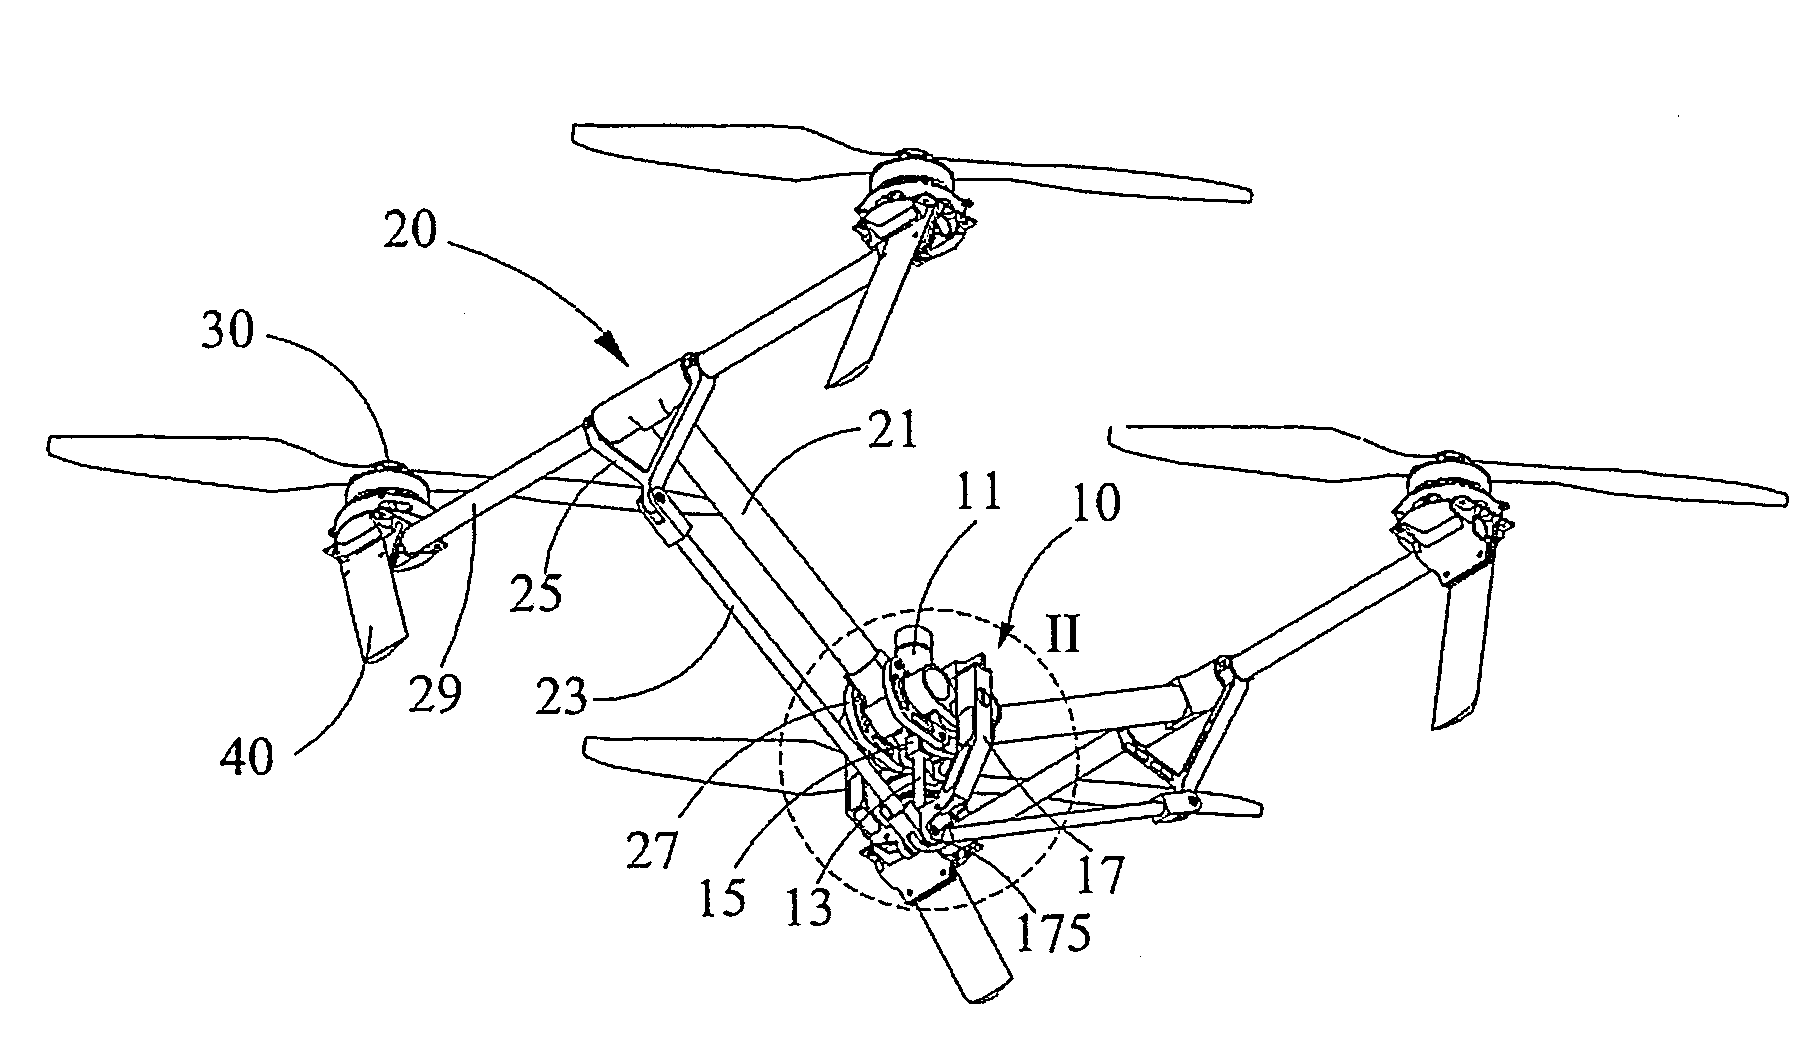
\includegraphics[width=\textwidth]{figs/dji-inspire1}
\caption{Inspire 1 articulated upwards}
\label{fig:inspireup}
\end{subfigure}%
\begin{subfigure}{.5\textwidth}
\centering
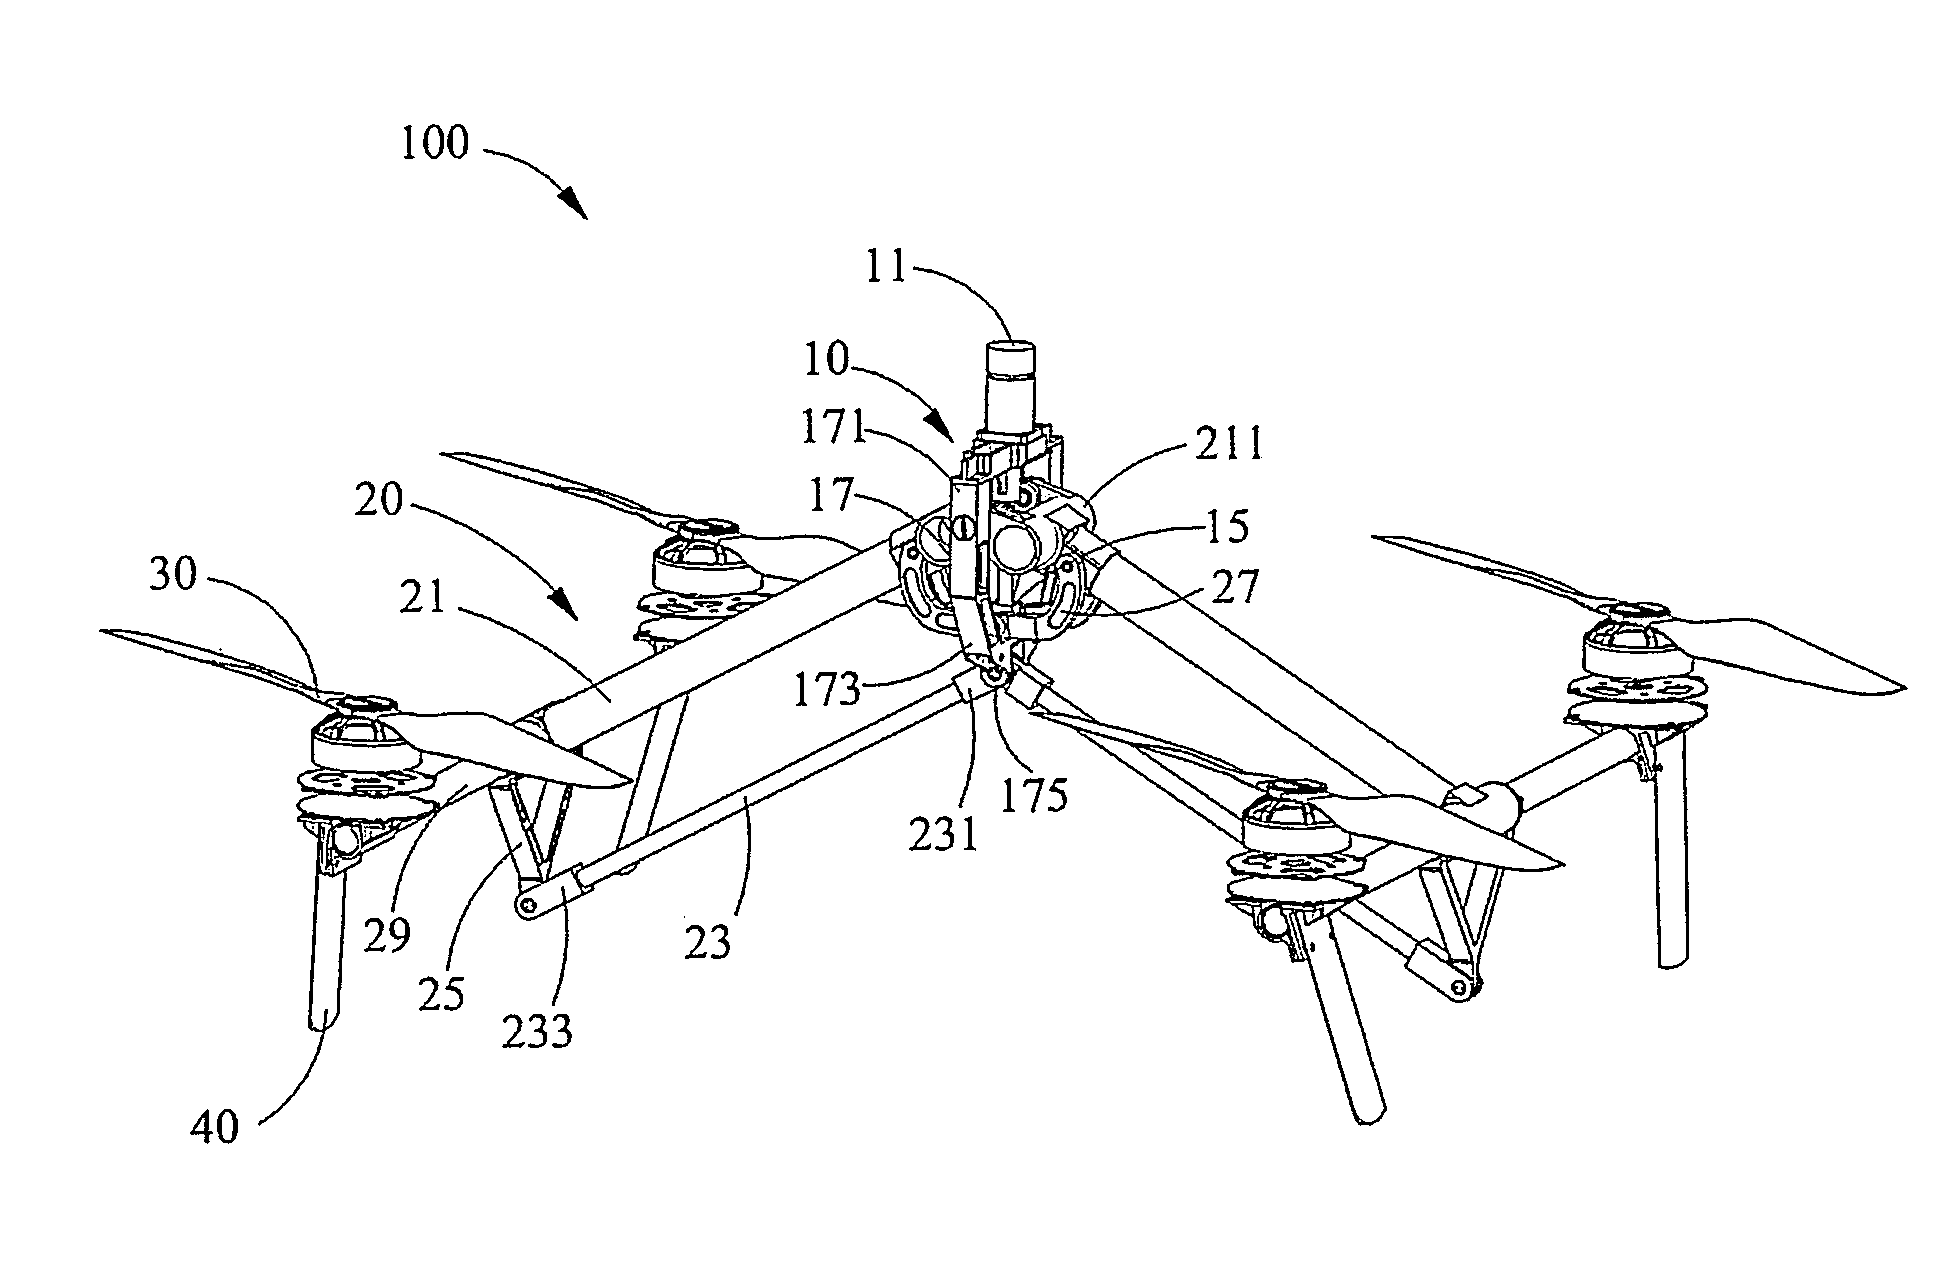
\includegraphics[width=\textwidth]{figs/dji-inspire2}
\caption{Inspire 1 articulated downwards}
\label{fig:inspiredown}
\end{subfigure}
\caption{DJI Inspire 1}
\label{fig:inspire1}
\end{figure}
\par
Another interesting project is that by G.Gres \cite{gres2007} which attempts to use oblique active tilting of a bi-rotor helicopter to induce gyroscopic torques. Whilst the eVader prototype referred to in the paper has dual axis tilting, the actuators are coupled together making the tilt axis 45\textdegree to the bodies' frame. The paper discusses in depth the mechanical system identification aspects of the prototype but, however, gives no insight into attitude control. The author instead discusses the dynamic equations of motion applicable in different flight modes. Whilst the later is irrelevant to quadrotor attitude control, the derivation of induced gyroscopic torque responses as a result of pitching the propellers from their principle plane of rotation is highly pertinent and appears to be the most accurate and well thought out of its' kind.
\par
Lastly, the most advanced implementation of over actuation for quadrotor control is that of Pau Segui Gasco \cite{tiltgasco}, which was a dual presented MSc project with Yazan Al-Rihani \cite{tiltrihani}. At the time of writing, this would appear to be the only published project which bears semblance to the proposed concept of this paper. The work was split between the two authors who completed the control/electronic design and the mechanical platform design for their respect MSc projects. Shown in Fig:\ref{fig:tiltrotor-gasco} \footnote{Development of a Dual Axis Tilt Rotorcraft UAV: Modelling, Simulation and Control \cite{tiltgasco}}, their dual-axis articulation is achieved with an adapted helicopter tail bracket, reducing the mass of the articulated component but limiting the range of rotation. Their justification for adding extra actuations is to ensure control reliability even in the event of losing up to 2 rotors.
\begin{figure}[hbtp]
\centering
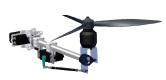
\includegraphics[width=0.7\textwidth]{figs/gasco-mech}
\caption{Dual-axis tilt-rotor mechanism}
\label{fig:tiltrotor-gasco}
\end{figure}
\par
In the control and dynamics derivation, Gesco et al provides an excellent model for 6-DOF motion. As is standard fare with quadrotor papers, the dynamic equations are linearised around a trim point parallel to the inertial frame to allow for SISO control analysis of the system. It is important to note the difference between this papers' prototype and the Bi-Directional Tilting Quadrotor Prototype developed in Chapter \cite{ch:design} ,the added actuation in \cite{tiltgasco} is not used to vector thrust produced but rather to leverage induced gyroscopic torques as an actuation input. The control allocation technique developed is wholly unique, fusing differential torque and torques induced from the relative motion with a (simplified) weighted pseudo inverse method. This all resulted in a control plant with a far higher control bandwidth. 
\par
In practice the gyroscopic response (see Section \ref{ch3:gyroscpic torque}), or rather regarding the spinning propellers as control moment gyroscopes \cite{cmg}, has a response two orders of magnitude smaller than that of the inertial response from pitching the mass of the motor \& propeller combination. And so such an inertial response is far more important to account for, weather it be compensation or exploitation, that the gyroscopic torques induced.
\subsection{Notable Quadrotor Control Implementations}
\label{subsec:ch1.lit.notablecontrol}
%----------------------------------------------------
The majority of papers based on Quadrotor research, \cite{quaddynamics},\cite{optimizedPID}, \cite{fourrotorrobot} all make the assumption that the coupled non-linear dynamics can be linearised. This assumptions holds true as long as the angular rate, $\vec{\Omega}$ is small and the inertial matrix, $\mathbb{I}$ is a diagonal matrix. As a consequence the gyroscopic term, (see \ref{ch:ch3}) which manifests itself as: $\tau _{gyro} = \vec{\Omega} \times \mathbb{I} \vec{\Omega} \approx \vec{0}$. This decouples the angular equations of motion and similarly the coriolis acceleration term becomes negligible; $-\vec{a} \times \vec{\Omega} \approx \vec{0}$.
\par
A PID strucuture for attitude controllers are the norm, with \cite{optimizedPID},\cite{quaddynamics},\cite{tiltpropellerflight} all implementing standard PID controllers and even \cite{singleaxistilting} using only a PD controller despite having an over-actuated platofrm. Even commercial hardware flight controllers like Arducopter\cite{arducopter} and OpenPilot \cite{openpilot}(whose firmware source code is available at \cite{openpilotgit}) all use PID structures with some manner of feedforward or feedback elements, \cite{buildyourownquad}.

However, in \cite{optimizedPID} the controller coefficients were selected through a learning social algorithm, a particle swarm optimization, instead of the regular "tuning" by hand. 
\par
As a result of the inherent singularity with using Rotation Matrices to represent attitude, 
%****************************************************
% END
%****************************************************

%****************************************************
%	CHAPTER 2 - Prototype Design
%****************************************************
\chapter{Prototype Design}
\label{ch:proto}
%====================================================
\section{Design}
\label{sec:proto.design}
%====================================================
\begin{figure}[htbp]
\centering
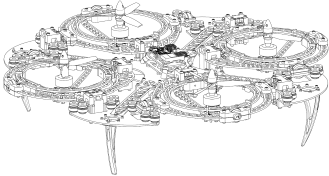
\includegraphics[width=0.93\textwidth]{figs/iso-design}
\caption{Isometric view of the prototype design}
\label{fig:iso-design}
\end{figure}
The final prototype (Fig:\ref{fig:iso-design}) went through a series of different design iterations, aimed at optimizing engineering time spent on construction and reducing the associated component costs. Significant consideration for the design process was the net weight whose upper limit is inherently limited by the thrust produced from lift motors. Some of the more important design factors, like inertial matrices and associated masses (Sec:\ref{sec:proto.inertia}), are discussed here in order to give context for the dynamics derived later in Ch:\ref{ch:dynamics}. The reference frame orientations (which those dynamics are developed with respect to) are detailed here. A brief overview of the electrical systems layout is then given with the components associated and their electrical characteristics included. Finally the actuator suite's functionality and transfer characteristics are quantified.
%====================================================
\subsection{Actuation Functionality}
\label{subsec:proto.design.actuation}
%====================================================
The most important component of the design is the articulation for each of the four vectored thrust forces. A concentric gimbal ring structure (Fig:\ref{fig:motor-assembly}) independently redirects each lift propeller/motor about two separate rotational axes. Within each module are servos affixed onto sequential gyroscope-like support rings to accommodate pitching and rolling of the propeller's direction. Aligned with each servo is a coaxial support bearing. The bearing and actuator servos have a mass disparity which results in an eccentric center of mass, producing a net gravitational torque arm. Unfortunately, due to weight constraints, counter balance measures cannot be introduced. Consequences from the center of mass variations must be either compensated for (\emph{plant dependent solution}) or exploited in the dynamics (\emph{additional nonlinear actuator plants}). The precise effects are quantified numerically later in Sec:\ref{sec:proto.inertia}.
\par
\begin{figure}[hbtp]
\begin{subfigure}{.49\textwidth}
\centering
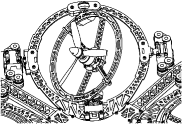
\includegraphics[width=\textwidth]{figs/motor-assembly}
\caption{Motor module assembly}
\label{fig:motor-assembly}
\end{subfigure}
\begin{subfigure}{.49\textwidth}
\centering
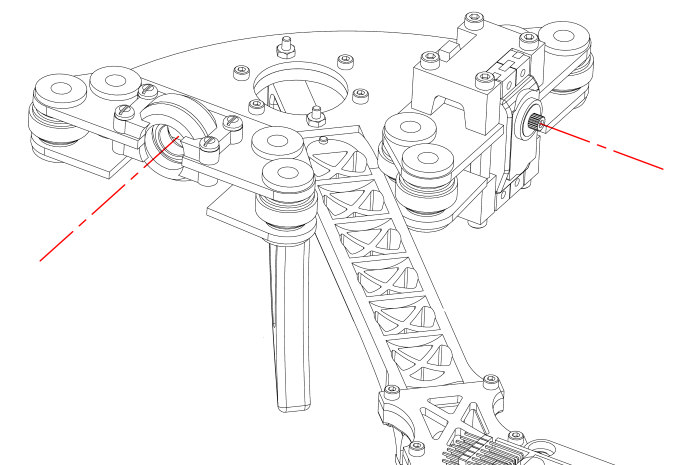
\includegraphics[width=\textwidth]{figs/motor-support}
\caption{Motor frame damping support assemblies}
\label{fig:motor_support}
\end{subfigure}
\caption{Tilting rotor design}
\end{figure}
Each motor module is positioned such that its produced thrust vector coincides with the intersection of its two rotational axes (Fig:\ref{fig:motor-assembly}). As a result there is only a perpendicular displacement of the thrust vector, $L_{arm}=195.16~\text{mm}$, co-planar to the body frame's X-Y-Z origin $\vec{\mathbf{O}}_b$ (see subsequent Fig:\ref{fig:motor-frame}). That length directly affects the differential torque plant; $\vec{\tau}_{diff}=\sum\vec{L}_i\times\vec{T}_i$. An eccentric thrust vector line would make the torque arm displacement a non-orthogonal vector. The center of gravity for each module is time varying and depends on the two servo rotational positions. It is more prudent to ensure intersection of the thrust vector with the rotational center than to balance the masses undergoing rotation. A thrust varying torque is harder to approximate and hence compensate for than a gravitational torque, given the complexity of modeling a propeller's aerodynamic thrust (Sec:\ref{subsec:dynamics.aero.bem}).
\par
The primary body structure is similar to a traditional quadcopter `+' configuration with adjacent propellers spinning in opposite directions. Each motor module's rotational assembly is suspended by silicone damping balls (Fig:\ref{fig:motor_support}). A smaller damping assembly in the center of the frame houses all the electronics and power distribution circuitry. All the mounting brackets affixing the motor module rings are 3D printed from CAD models using an Ultimaker V2+\cite{ultimaker}. A complete bill of materials for all parts used, including working drawings for each 3D printed bracket and the laser cut frame(s), is presented in App:\ref{app:bom}.
\par
\begin{figure}[hbtp]
\centering
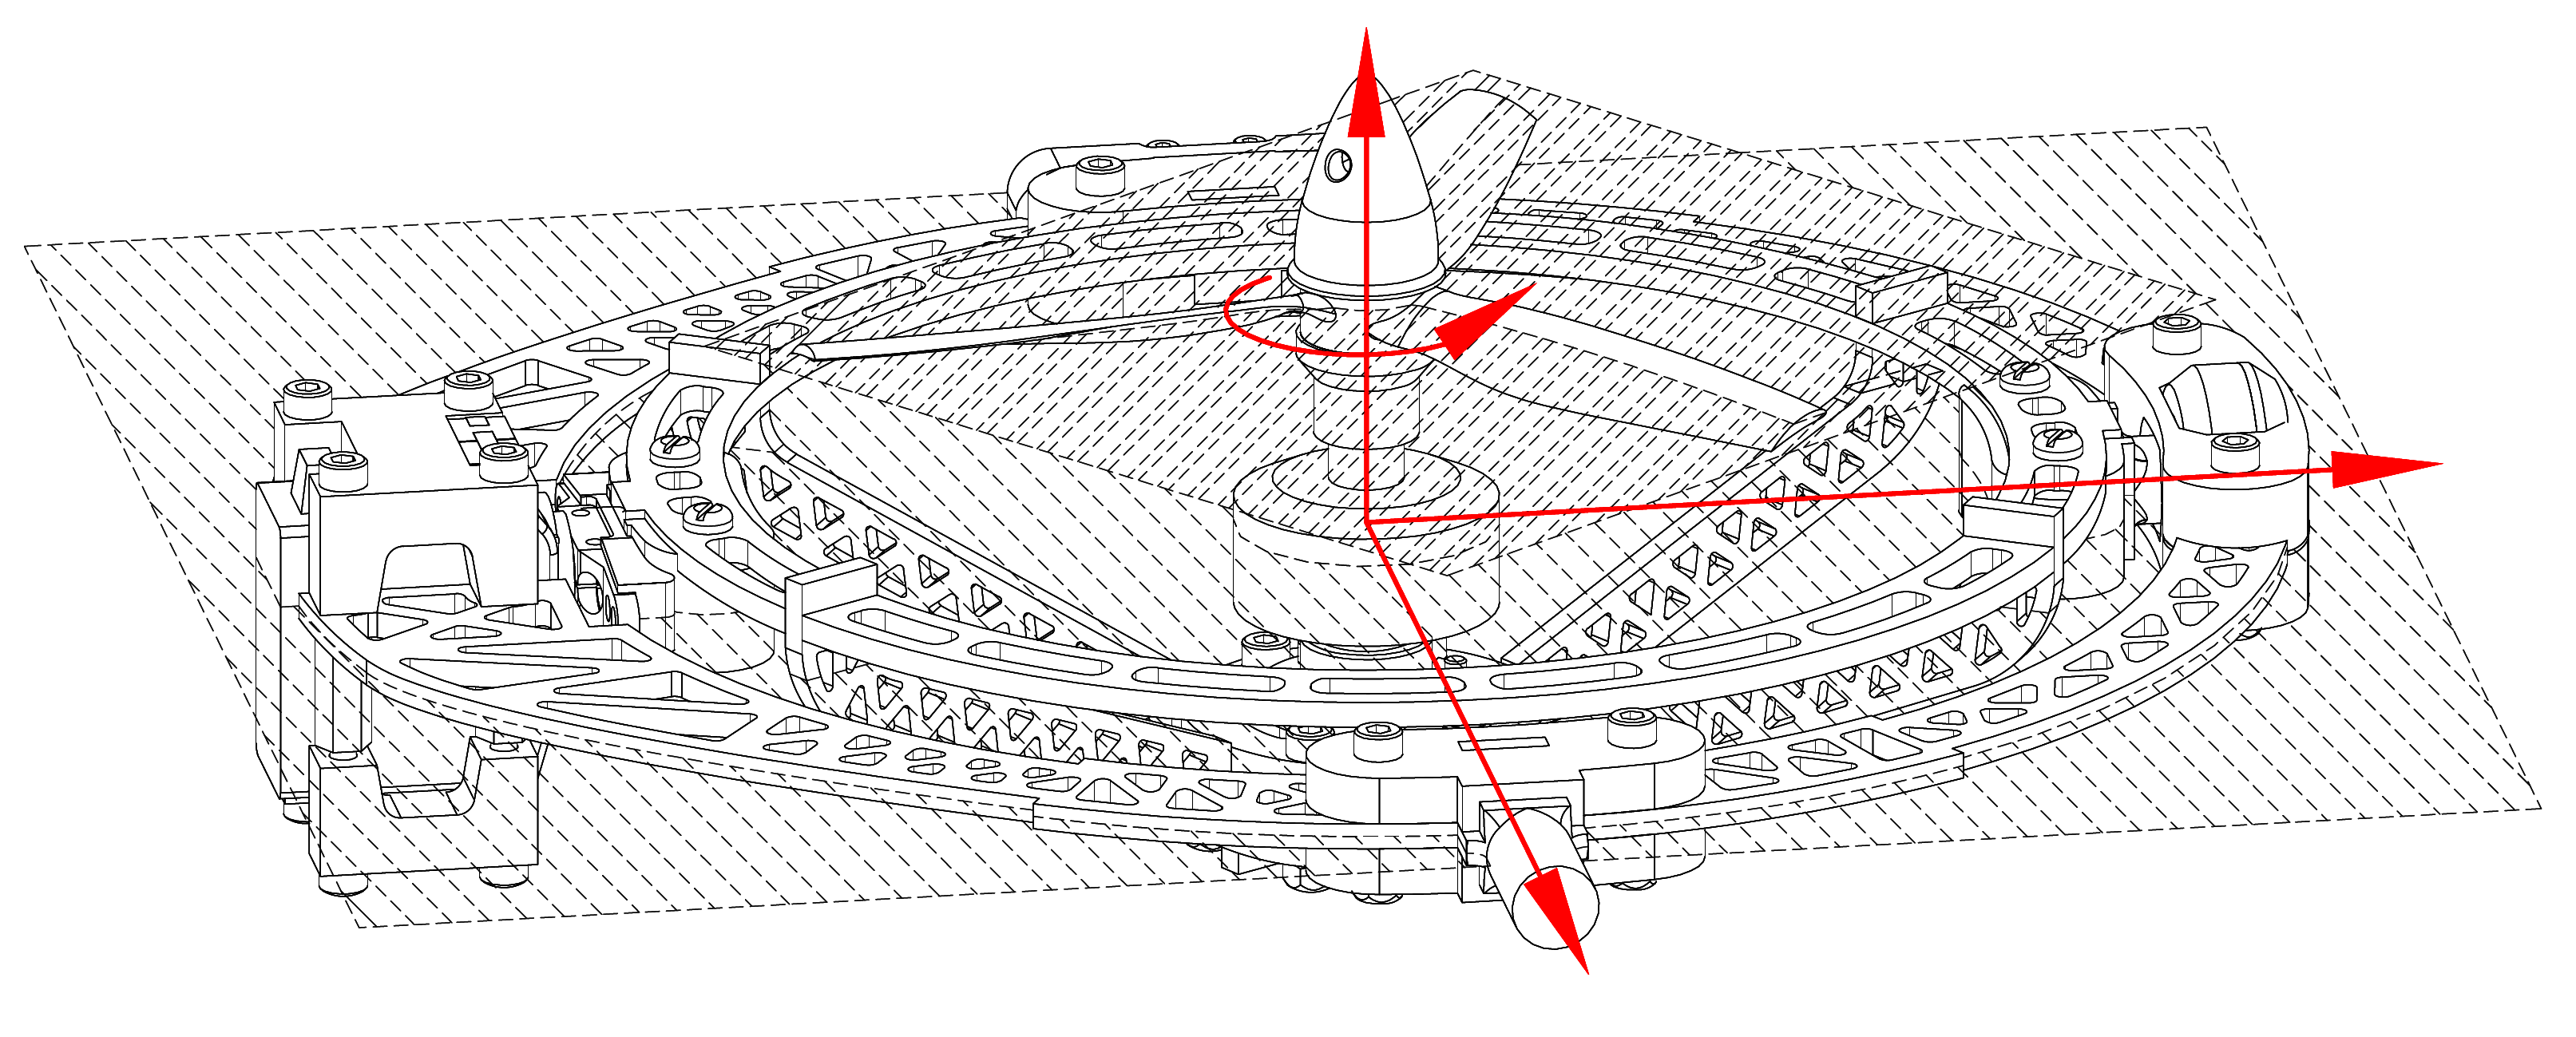
\includegraphics[width=0.85\textwidth]{figs/motor-prop}
\vspace{-10pt}
\caption{Difference between propeller and motor planes}
\label{fig:motor_prop}
\vspace{-15pt}
\end{figure}
The propeller's rotational plane is not aligned exactly with the plane made by the $\hat{X}_{M_i}$ and $\hat{Y}_{M_i}$ rotational servo axes (Fig:\ref{fig:motor_prop}). The offset is approximately $23.0~\text{mm}$ and must be considered when evaluating pitch/roll inertial and gyroscopic torque responses later in Sec:\ref{subsec:dynamics.nonlinearities.gyrotorques}. The propellers are six inch ($6 \times 4.5$) three-bladed plastic Gemfam propellers, powered by Cobra CM2208-2000 KV Brushless DC motors (Fig:\ref{fig:bldc-motor}). The thrust produced as a function of angular velocity (in revolutions per second) for the propellers is derived in Sec:\ref{subsec:dynamics.aero.bem}. 
\newpage
The BLDC motors are controlled with LDPower 20A ESC modules with an in-line OrangeRx RPM Sensor. The ESCs were reflashed with BLHeli\cite{BLHeli} firmware. The default firmware on the speed controllers had an unsatisfactory exponentially approaching, nonlinear input speed curve; in contrast with the linear unloaded speed curve in Fig:\ref{fig:rpm-sensor}. The net transfer functions for both ESC modules and the servos are detailed later in Sec:\ref{subsec:proto.design.transfer}. Power for the quadrotor is supplied from a power tether (not from a battery bank). Tethered power will ensure consistent flight time and reduce the concern of payload restriction on the available lift actuation. Power lines to both the BLDC motors and servos are supplied through conventional wiring, however an ideal and more flexible design would see slip-rings for each module's power supply. 
\begin{figure}[htbp]
\centering
\begin{subfigure}{0.49\textwidth}
\centering
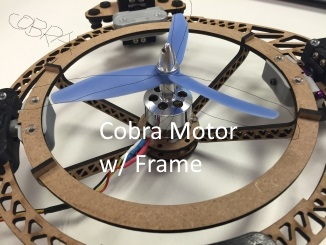
\includegraphics[width=0.9\textwidth]{figs/motor-bldc}
\caption{Cobra CM2208-2000KV BLDC motor module}
\label{fig:bldc-motor}
\end{subfigure}
\begin{subfigure}{0.49\textwidth}
\centering
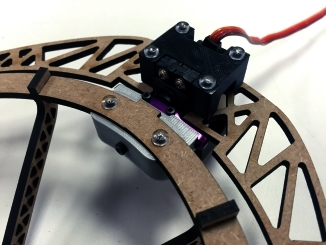
\includegraphics[width=0.9\textwidth]{figs/motor-servo}
\caption{Corona DS-339MG servo bracket}
\label{fig:motor-servo}
\end{subfigure}
\vspace{-5pt}
\caption{Motor module assembly}
\vspace{-15pt}
\end{figure}
\par
Metal gear Corona DS-339MG digital servos are used for the two axes of rotation (Fig:\ref{fig:motor-servo}). Each servo has a rotational range of $\approx 180\text{\textdegree}$, positioned such that a $\text{zero}^{\text{th}}$ offset aligns the motor modules, adjacent to the body frame, and has a $\pm 90\text{\textdegree}$ rotational range. A digital servo updates at 330 Hz, faster than a 50 Hz analogue servo equivalent (Fig:\ref{fig:servo-timing}). This means the otherwise $20~\text{ms}$ zero-order ``analogue" sampling effect is a less significant $3.30~\text{ms}$ zero-order holding time. Both the $\hat{X}_{M_i}$ and $\hat{Y}_{M_i}$ axis servos will be rotating differing inertial bodies; as such their open loop transfer functions are individually determined through testing in Sec:\ref{subsec:proto.design.transfer}.
\begin{figure}
\centering
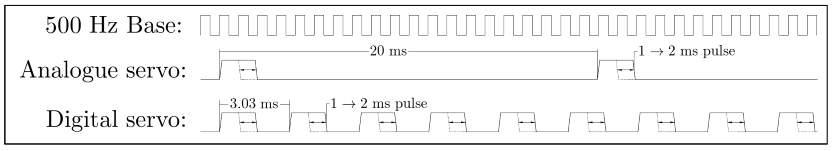
\includegraphics[width=0.75\textwidth]{figs/servo-timing}
\caption{Digital and analogue servo timing}
\label{fig:servo-timing}
\vspace{-20pt}
\end{figure}
%====================================================
\section{Reference Frames Used}
\label{sec:proto.conventions}
Attitude conventions used for deriving the system's dynamics in Ch:\ref{ch:dynamics}~are first discussed here. Often these aspects are assumed to be obvious enough that they are omitted. It is important to clearly and unambiguously define a standard set of framing conventions to avoid uncertainty later. Rotation matrices are included but the focus is on the \emph{contrast} between rotation and transformation operations. Both \cite{spacecraftattitutdequaternions} and \cite{rigidbodylecture} provide an in-depth and thorough explanation of rotation matrices and direct cosine matrix attitude representation, if such concepts are unfamiliar to the reader. Later quaternions are used to replace rotation matrix notation for the dynamics in Sec:\ref{subsec:dynamics.rigidbody.quaternion}.
%====================================================
\subsection{Reference Frames Convention}
\label{subsec:proto.conventions.frames}
%====================================================
\begin{figure}[htbp]
\centering
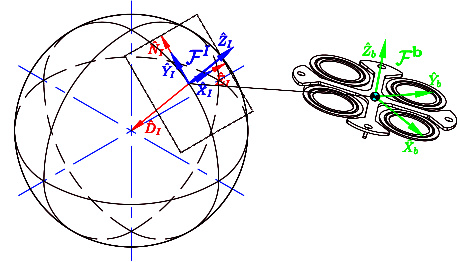
\includegraphics[width=0.8\textwidth]{figs/reference-frame}
\caption{Inertial and body reference frames}
\label{fig:ref_frame}
\end{figure}
NASA aerospace frames are used for principle Cartesian inertial and body coordinate representation (Fig:\ref{fig:ref_frame}). The inertial frame,~$\mathcal{F}^I$ with an origin $\vec{\mathbf{O}}_I$, is aligned such that the $\hat{Y}_I$ axis is in the $\hat{N}$orth direction, $\hat{X}_I$ is in the $\hat{E}$ast direction and $-\hat{Z}_I$ is  in the $\hat{D}$ownward direction. In Euler orbital sequences the $\hat{Z}$ direction would be toward the Earth's center, sometimes referred to as the N\^{E}D convention which differs from the NASA frames used here. The body frame, $\mathcal{F}^b$ centered on the point $\vec{\mathbf{O}}_b$, then has both $\hat{X}_b$ and $\hat{Y}_b$ aligned obliquely between two perpendicular arms of the quadrotor's body and the $\hat{Z}_b$ axis in the body's normal upward direction (illustrated in Fig:\ref{fig:body-frame}). 
\par
The body frame's axes and center of motion relative to the prototype design's center of mass are both detailed next in Sec:\ref{subsec:proto.conventions.motoraxis}. Frame superscripts $I$ and $b$ represent inertial and body frames respectively whilst vector subscripts imply the reference frame in which the vector's coordinates exists or taken relative to. The function $R_I^b(\eta)$ represents a rotation operator of the Euler set $\vec{\eta}$ (expanded on in Eq:\ref{eq:inertialbodytransformation}) rotating from subscript frame $\mathcal{F}^I$ to superscript frame $\mathcal{F}^b$. 
\par
A vector $\vec{\nu}$ has the relationship between the body and inertial frames:
\begin{equation}
\vec{\nu}_I=R_b^I(\eta)\vec{\nu}_b~~~~~~\vec{\nu}_b\in\mathcal{F}^b,~\vec{\nu}_I\in\mathcal{F}^I
\end{equation}
Displacement between the inertial and body frames is given by $\vec{\mathcal{E}}_I$ defined in the inertial frame:
\begin{equation}\label{eq:position-frame}
\vec{\mathcal{E}}_I=\begin{bmatrix}
x & y & z\end{bmatrix}^T~~~~\in\mathcal{F}^I
\end{equation}
An axial hat and upper case differentiates axis unit vectors $\hat{X},\hat{Y},\hat{Z}$ from inertial position quantities $x,y,z$ in Eq:\ref{eq:position-frame}. The body position's time derivative $\dot{\vec{\mathcal{E}}}_I$ refers to the \emph{inertial frame} rate:
\begin{equation}
\frac{d}{dt}\vec{\mathcal{E}}_I=\begin{bmatrix}
\dot{x} & \dot{y} & \dot{z}\end{bmatrix}^T~~~~\in\mathcal{F}^I
\end{equation}
Whereas the body's translational velocity $\vec{v}_b$ is with respect to the body frame $\mathcal{F}^b$. Velocity and the inertial position time derivative are related as follows:
\begin{subequations}
\begin{equation}
\vec{v}_b=R_I^b(\eta)\dot{\vec{\mathcal{E}}}_I~~~~\in\mathcal{F}^b
\end{equation}
\vspace{-18pt}
\begin{equation}
=R_I^b(\eta)\begin{bmatrix}
\dot{x} & \dot{y} & \dot{z}
\end{bmatrix}^T~~~~
\end{equation}
\end{subequations}
Relative angular displacement between two frames is commonly measured by the three angle Euler set. The Euler angle set $\vec{\eta}=[\phi ~\theta ~\psi]^T$ represents pitch $\phi$, roll $\theta$ and yaw $\psi$ rotations about sequential $\hat{X}$,$\hat{Y}$ and $\hat{Z}$ axes respectively. Depending on how the rotation sequence is formulated, those angles can be used to construct rotation matrices which give relation to vectors or can transform coordinates. 
\par
The general rotation equation to \emph{rotate} some vector $\vec{\nu}$ about a normalized unit axis $\hat{u}$ through a rotation angle $\theta$ is given by the rotation formula, derivated in \cite{rigidbodymotion}:
\begin{equation}\label{eq:genrotationmatrix}
\vec{\nu}~'=\big(1-cos(\theta)\big)\big(\vec{\nu}\cdot \hat{u}\big)\hat{u}+cos(\theta)\vec{\nu}+sin(\theta)\big(\hat{u}\times\vec{\nu}\big)
\end{equation}
In Eq:\ref{eq:genrotationmatrix}, when the unit vector $\hat{u}$ is in the direction of either $\hat{X}$; $\hat{Y}$ or $\hat{Z}$ axes the equation is simplified to produce the three fundamental rotation matrices $R_x(\phi)$; $R_y(\theta)$ and $R_z(\psi)$. That set of three principle rotation matrices about the Cartesian X-Y-Z axes are defined as:
\begin{subequations}\label{eq:rotationmatrix}
\begin{equation}
R_x(\phi)=\begin{bmatrix}
1 & 0 & 0\\
0 & cos(\phi) & -sin(\phi)\\
0 & sin(\phi) & cos(\phi)
\end{bmatrix}
\end{equation}
\vspace{-2pt}
\begin{equation}
R_y(\theta)=\begin{bmatrix}
cos(\theta) & 0 & sin(\theta)\\
0 & 1 & 0\\
-sin(\theta) & 0 & cos(\theta)
\end{bmatrix}
\end{equation}
\begin{equation}
R_z(\psi)=\begin{bmatrix}
cos(\psi) & -sin(\psi) & 0\\
sin(\psi) & cos(\psi) & 0\\
0 & 0 & 1
\end{bmatrix}
\end{equation}
\end{subequations}
The notation for a rotation matrix operation is multiplication of the matrix $R_{u}(\theta)$, applying a left-handed \emph{rotation} operator about some axis $\hat{u}$ by $\theta$. The resultant vector of a rotation operation still exists in the same reference frame. For example an $\hat{X}$ axis rotation by $\phi$ of some vector $\vec{\nu}$ is given by:
\begin{subequations} \label{eq:rotationoperator}
\begin{equation}\label{eq:rotationoperator.a}
\vec{\nu}^{\hspace{1pt}}\text{}'=R_{x}(\phi)\vec{\nu}~~~~~\vec{\nu}^{\hspace{2pt}}\text{}',\vec{\nu}\in\mathcal{F}^1
\end{equation}
\end{subequations}
No subscripts are used in Eq:\ref{eq:rotationoperator} to indicate reference frame ownership because all vectors are in the same frame. The time derivative of a rotation matrix about some axis $\hat{u}$ by a rotation $\theta$, $\dot{R}_u(\theta)$ is shown in \cite{quaddynamics} to be:
\begin{subequations}\label{eq:rotation-matrix-derivative}
\begin{equation}
\frac{d}{dt}\big(R_u(\theta)\big)=\big(\dot{\theta}\cdot\hat{u}\big)\times R_u\Rightarrow\big[\dot{\theta}\cdot\hat{u}\big]_{\times}R_u
\end{equation}
Where $\dot{\theta}\cdot\hat{u}$ is the projection of the angular rate $\dot{\theta}$ onto the $\hat{u}$ axis. Furthermore, for some vector $\vec{a}$, the operator $[\vec{a}\hspace{1pt}]_\times$ denotes the cross-product matrix or \emph{skew} matrix. The symmetric skew matrix is a matrix multiplication to replace the cross-product operator, for some other vector $\vec{b}$;
\begin{equation}
\vec{a}\times\vec{b}\equiv\big[\vec{a}\hspace{1pt}\big]_\times\vec{b}
\end{equation}
\vspace{-12pt}
\begin{equation}\label{eq:cross-product-matrix}
\rightarrow\big[\vec{a}\big]_\times\triangleq\begin{bmatrix}
0 & -a_3 & a_2\\
a_3 & 0 & -a_1\\
-a_2 & a_1 & 0
\end{bmatrix}
\end{equation}
\end{subequations}
A vector \emph{transformation} changes the resultant vector's reference frame. The transformation is then a rotation by an angle of the \emph{difference} (or negative angle) between the resulting and principle reference frames. A transformation from frame $\mathcal{F}^1$ to $\mathcal{F}^2$, differing by an angle of $\phi$ about the $\hat{X}$ axis is then a negative rotation operation:
\begin{subequations}\label{eq:transformationoperator}
\begin{equation}\label{eq:transformationoperator.a}
\vec{\nu}_2=R_x(-\phi)\vec{\nu}_1
\end{equation}
\vspace{-15pt}
\begin{equation}\label{eq:transformationoperator.b}
\vec{\nu}_2\in\mathcal{F}^2~\text{and}~\vec{\nu}_1\in\mathcal{F}^1
\end{equation}
\end{subequations}
The distinction between Eq:\ref{eq:rotationoperator} and Eq:\ref{eq:transformationoperator} is the directional sense of the angular operand $\phi$, and hence the effect it has on the argument vector. The transformation or rotation of a vector from the inertial frame $\mathcal{F}^I$ to the body frame $\mathcal{F}^b$ is the product of three sequential operations about each princple axis. Each subsequent rotation is applied relative to a new intermediate frame; hence each Euler angle is taken relative to a specific intermediate frame and not a global one. The order of those axial rotation operations does affect the Euler set, any consequences of which are detailed in \cite{rotationsequences}. In this dissertation the Z-Y-X or yaw, pitch, roll rotation sequence is used. A rotation of the vector $\vec{\nu}$ from the inertial to the body frame, $\mathcal{F}^I\rightarrow\mathcal{F}^b$, is then applied by sequential yaw, $\psi$, pitch, $\theta$, and roll $\phi$ operations about the $\hat{Z},~\hat{Y}$ and $\hat{X}$ axes respectively:
\begin{subequations}\label{eq:inertialbodyrotation}
\begin{equation}\label{eq:inertialbodyrotation.a}
R_I^{b}(\eta)=R_{I}^{b}(\phi,\theta,\psi)\triangleq R_z(\psi)R_y(\theta)R_x(\phi)
\end{equation}
\vspace{-14pt}
\begin{equation}\label{eq:inertialbodyrotation.b}
\vec{\nu}^{\hspace{1pt}}\text{}'=R_I^b(\phi,\theta,\psi)\vec{\nu}
\end{equation}
\vspace{-12pt}
\begin{equation}\label{eq:inertialbodyrotation.c}
\rightarrow\vec{\nu}^{\hspace{1pt}}\text{}'=R_z(\psi)R_y(\theta)R_x(\phi)\vec{\nu}
\end{equation}
\end{subequations}
It is important to note that in Eq:\ref{eq:inertialbodyrotation} both operand and output vectors are \emph{both} in the inertial frame, namely $\vec{\nu}^{\hspace{2pt}}\text{}'~,\vec{\nu}\in\mathcal{F}^I$. A \emph{transformation} of a vector from the inertial to the body frame is the negative counterpart of Eq:\ref{eq:inertialbodyrotation}, a distinction which is not always explicitly stated.
\begin{subequations}\label{eq:inertialbodytransformation}
\begin{equation}\label{eq:inertialbodytransformation.a}
\vec{\nu}_b=R_I^b(-\eta)\vec{\nu}_I=R_I^b(-\phi,-\theta,-\psi)\vec{\nu}_I
\end{equation}
\vspace{-12pt}
\begin{equation}\label{eq:inertialbodytransformation.b}
\text{for}~~\vec{\nu}_b\in\mathcal{F}^b~\text{and}~~\vec{\nu}_I\in\mathcal{F}^I
\end{equation}
\vspace{-10pt}
\begin{equation}\label{eq:inertialbodytransformation.c}
\rightarrow \vec{\nu}_b=R_z(-\psi)R_y(-\theta)R_x(-\phi)\vec{\nu}_I
\end{equation}
\vspace{-10pt}
\begin{equation}\label{eq:inertialbodytransformation.d}
=R_x(\phi)R_y(\theta)R_z(\psi)\vec{\nu}_I=R_{b}^{I}\vec{\nu}_I
\end{equation}
\vspace{-8pt}
\begin{equation}\label{eq:inertialbodytransformation.e}
R_I^b=\big(R_b^I\big)^{-1}=\big(R_b^I\big)^T
\end{equation}
\end{subequations}
The relationship in Eq:\ref{eq:inertialbodytransformation.e} is an inversion property (\emph{transpose}) of the rotation matrix. A rotation matrix's inverse can be used interchangeably with its negative counterpart to maintain a positive sense of the argument angle. To ensure clarity throughout this dissertation's mathematics, a negative angular sense implies a \emph{transformation} to a different reference frame. Where applicable, the order of rotation will indicate the sequence direction whilst the angular sign differentiates the rotation or transformation operations.
\par
The body frame's angular velocity is taken relative to the inertial frame, represented by $\vec{\omega}_{b/I}$ mostly just simplified to $\vec{\omega}_b$. Seeing that each Euler angle is measured with respect to an intermediary frame, a distinction must then be made between $d\vec{\eta}/dt$ and $\vec{\omega}_b$. All three Euler angles need to be transformed to a common frame to define the relationship between Euler and angular rates. Exploiting vehicle frames 1 \& 2, or rather $\mathcal{F}^{v1}$ \& $\mathcal{F}^{v2}$, as intermediary frames to retrospectively describe frames after $R_x(\phi)$ and $R_y(\theta)$ operations and using the rotation matrix derivative from Eq:\ref{eq:rotation-matrix-derivative}. The angular velocity $\vec{\omega}_b$ is the time derivative of Euler angles in the body frame:
\begin{subequations}\label{eq:angular-rates-eq}
\begin{equation}\label{eq:angular-rates.a}
\vec{\omega}_b=\begin{bmatrix}
p & q & r
\end{bmatrix}^T
\triangleq
\frac{d}{dt_b}\vec{\eta}=\frac{d}{dt}\vec{\eta}_b~~~~\in\mathcal{F}^b
\end{equation}
\vspace{-8pt}
\begin{equation}\label{eq:angular-rates.b}
\vec{\eta}_b \triangleq R_{v_2}^b(\phi)\hspace{2pt}\vec{\phi}+R_{v_2}^b(\phi)R_{v_1}^{v_2}(\theta)\hspace{2pt}\vec{\theta}+R_{v_2}^b(\phi)R_{v_1}^{v_2}(\theta)R_I^{v_1}(\psi)\hspace{2pt}\vec{\psi}~~~~\in\mathcal{F}^b
\end{equation}
\vspace{-4pt}
\begin{equation}\label{eq:angular-rates.c}
\therefore\vec{\omega}_b=\begin{bmatrix}
\dot{\vec{\phi}}~
\end{bmatrix}_\times\hspace{-3pt}R_{v2}^b(\phi)+R_{v2}^{b}(\phi)\begin{bmatrix}
\dot{\vec{\theta}}~
\end{bmatrix}_\times\hspace{-3pt}R_{v1}^{v2}(\theta)+ R_{v2}^{b}(\phi)R_{v1}^{v2}(\theta)\begin{bmatrix}
\dot{\vec{\psi}}
\end{bmatrix}_\times\hspace{-3pt}R_{I}^{v1}(\psi)~~~~\in\mathcal{F}^b
\end{equation}
With Euler vectors $\vec{\phi},~\vec{\theta}$ and $\vec{\psi}$ being axis projections onto X-Y-Z axes respectively; $\phi\cdot\hat{\imath},~\theta\cdot\hat{\jmath}$ and $\psi\cdot\hat{k}$. The vehicle frames used for Eq:\ref{eq:angular-rates.a} and the subsequent rotations between each frame don't necessarily have to be in that order. The equation could change depending on what rotation sequence was used, here Z-Y-X rotation sequences was use. The Euler rate Eq:\ref{eq:angular-rates.c} then simplifies to the formal relationship between two rotating frames, with $\vec{\omega}_b=[p~q~r]^T$:
\begin{equation}\label{eq:angular-rates.b}
\begin{bmatrix}
p\\
q\\
r\\
\end{bmatrix}
=
\begin{bmatrix}
1 & 0 & -sin(\theta)\\
0 & cos(\phi) & sin(\phi)cos(\theta)\\
0 & -sin(\theta) & cos(\phi)sin(\theta)\\
\end{bmatrix}
\begin{bmatrix}
\dot{\phi}\\
\dot{\theta}\\
\dot{\psi}\\
\end{bmatrix}
\end{equation}
\vspace{-8pt}
\begin{equation}\label{eq:angular-rates.c}
\Rightarrow\vec{\omega}_b=\Psi(\eta)\dot{\vec{\eta}}~~~~\in\mathcal{F}^b
\end{equation}
\vspace{-8pt}
\begin{equation}\label{eq:angular-rates.d}
\Psi(\eta)=
\begin{bmatrix}
1 & 0 & -sin(\theta)\\
0 & cos(\phi) & sin(\phi)cos(\theta)\\
0 & -sin(\theta) & cos(\phi)sin(\theta)\\
\end{bmatrix}
\end{equation}
\vspace{-2pt}
\begin{equation}\label{eq:angular-rates.e}
\Rightarrow\dot{\vec{\eta}}=\Psi^{-1}(\eta)\vec{\omega}_b=\Phi(\eta)\vec{\omega}_b~~~~\in\mathcal{F}^{v1,v2,I}
\end{equation}
\vspace{-4pt}
\begin{equation}\label{eq:angular-rates.f}
\Phi(\eta)=\begin{bmatrix}
1 & sin(\phi)tan(\theta) & cos(\phi)tan(\theta)\\
0 & cos(\phi) & -sin(\phi)\\
0 & sin(\phi)sec(\theta) & cos(\phi)sec(\theta)\\
\end{bmatrix}
\end{equation}
\end{subequations}
\par
The \emph{Euler} matrix, $\Psi(\eta)$, contains a well known and problematic singularity; at $\theta=\pm\pi/2$ where the determinant of the transformation matrix is zero. The mathematical manifestation of that singularity and its physical consequences are expanded on in Sec:\ref{subsec:dynamics.rigidbody.singularity}. The singularity is present in the middle roll angle $\theta$, which is a direct consequence of the chosen Z-Y-X rotation sequence adopted. Each Euler angle is potentially singular depending on the rotation order used. In later dynamics quaternions are used in lieu of Euler angles (Sec:\ref{subsec:dynamics.rigidbody.quaternion}). Attitude in $\mathbb{R}^3$, or $SO(3)$, is intuitive and well suited to the conventions defined here.
\par
Quaternions (Sec:\ref{subsec:dynamics.rigidbody.quaternion}), despite being in $\mathbb{R}^4$, are similarly constructed in the Z-Y-X order following a three rotation sequence. Combined quaternion operations are additive but non-commutative, as such the order is important. The constructed attitude quaternion order will produce the same resultant frame orientation however the quaternion, and its rotation path, will differ. A quaternion $Q_b$, representing the body's attitude, and some vector $\vec{\nu}_I$ in the inertial frame is related to the body frame $\mathcal{F}^b$ as follows:
\begin{subequations}
\begin{equation}\label{eq:quaternion-rotation-equivalence}
\vec{\nu}_b=R_I^b(-\eta)\vec{\nu}_I\underset{Q}{\iff} Q_b \otimes \begin{bmatrix}
0 & \vec{\nu}_I
\end{bmatrix}^T \otimes Q_b^*
\end{equation}
\vspace{-12pt}
\begin{equation}
Q_b \triangleq Q_z \otimes Q_y \otimes Q_x~~\text{and it's inverse}~~Q_b^* \triangleq Q_x^*\otimes Q_y^*\otimes Q_z^*
\end{equation}
\end{subequations}
The symbol $\otimes$ represents the Hamilton product, or quaternion multiplication operator. Later the Hamilton product is used again for inertial tensor transformations (Sec:\ref{sec:proto.inertia}). Each quaternion, $Q_{\hat{\imath}}$, is always the \emph{unit} quaternion about the $\hat{\imath}^{th}$ axis. For the body quaternion, $Q_b$, it is the unit quaternion rotation about the body's Euler axis, \cite{rotationsequences}. A quaternion rotation operates on an argument vector with a zero quaternion scalar component. So then for some vector $\vec{\nu}$, the quaternion rotation operation in Eq:\ref{eq:quaternion-rotation-equivalence} is equivalent to;
\begin{subequations}
\begin{equation}\label{eq:quaternion-operator.a}
Q_{\vec{\nu}^{\hspace{1pt}}\text{}'}=Q \otimes (Q_{\vec{\nu}}) \otimes Q^*
\end{equation}
\vspace{-14pt}
\begin{equation}\label{eq:quaternion-operator.b}
\text{Where}~Q_{\vec{\nu}}=\begin{bmatrix}
0 & \vec{\nu}~\end{bmatrix}^T,~~Q_{\vec{\nu}^{\hspace{1pt}}\text{}'}=\begin{bmatrix}
0&\vec{\nu}^{\hspace{1pt}}\text{}'~\end{bmatrix}
\end{equation}
\end{subequations}
Quaternion representation in Eq:\ref{eq:quaternion-operator.b} ensures that the operation is entirely in $\mathbb{R}^4$ space. However it is typically omitted, despite $\mathbb{R}^4$ being implied and as such, Eq:\ref{eq:quaternion-operator.a} is then simply:
\begin{equation}
\vec{\nu}^{\hspace{1pt}}\text{}'=Q \otimes (\vec{\nu}\hspace{2pt}) \otimes Q^*
\end{equation}
Quaternion dynamics, and the quaternion operator, are later expanded upon to replace the use of Euler angles and rotation matrices as a convention for attitude representation later in Chapter:\ref{ch:dynamics}.
\newpage
%====================================================
\subsection{Motor Axis Layout}
\label{subsec:proto.conventions.motoraxis}
%====================================================
The whole structure (previously in Fig:\ref{fig:iso-design}) consists of multiple rigidly connected bodies with only relative rotations between each body permitted by its revolute joints, illustrated previously in the design description in Sec:\ref{sec:proto.design}. Those rigid bodies are categorized into four inter-connected motor modules, $\mathbf{M}_{1\rightarrow 4}$, and a single body structure, $\mathbf{B}$ (\emph{frame} structure, not reference frame). Each module contains two sequential gimbal rings, where each ring has one degree of relative rotation, actuated by a servo, between itself and the subsequent ring. There needs to be distinct nomenclature used for describing these motor modules such that the dynamic derivations later are clear and logical despite the complicated multibody system\ldots
\par
\begin{figure}[htbp]
\vspace{-6pt}
\centering
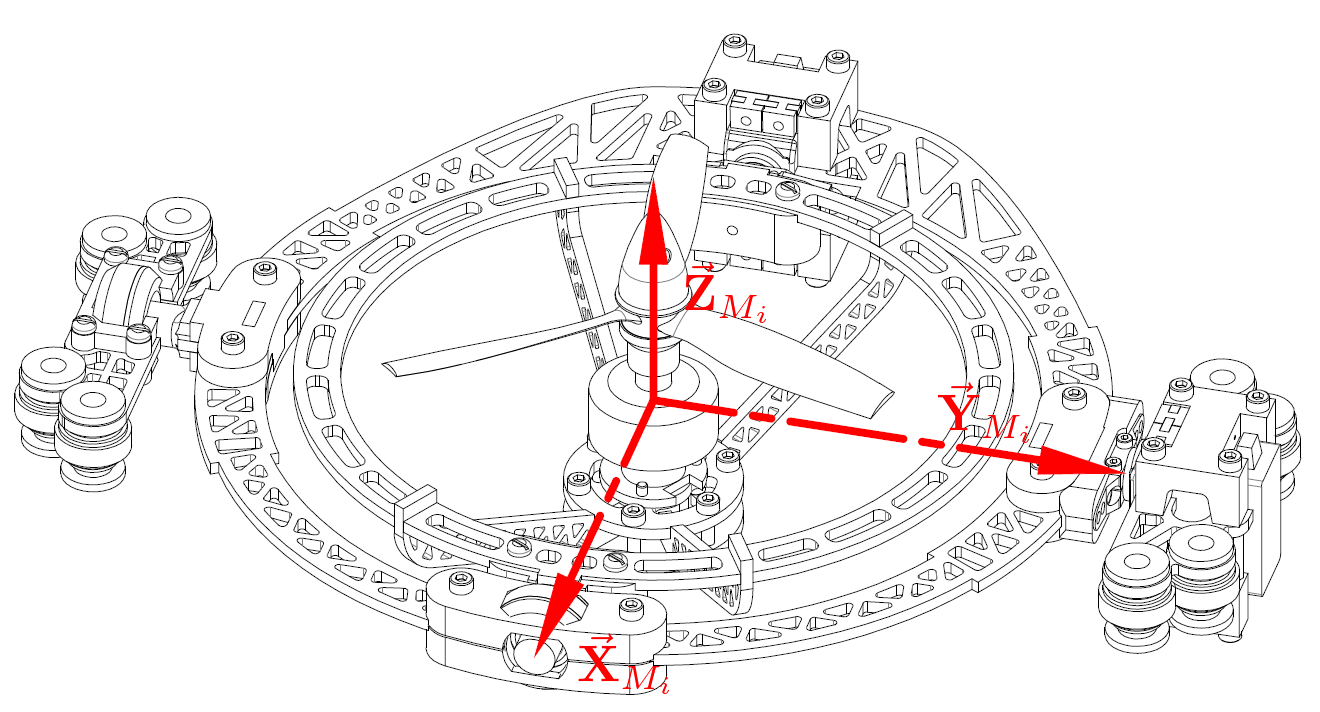
\includegraphics[width=0.85\textwidth]{figs/motor-axes}
\caption{Aligned motor frame axes}
\label{fig:motor-axes}
\vspace{-6pt}
\end{figure}
Every propeller/motor is actuated by a pair of two servos about two subsequent rotational axes (Fig:\ref{fig:motor-axes}) in a similar fashion to an Euler rotation sequence. A frame module frame $\mathcal{F}^{M_i}$ is attached to the innermost ring, the BLDC motor's stator is affixed to that frame and its rotor has a rotational velocity $\Omega_i$ about the $\hat{Z}_{M_i}$ stator axis. Fig:\ref{fig:motor-frame} shows the sequential relative module frames.
\begin{figure}[hbtp]
\vspace{-10pt}
\centering
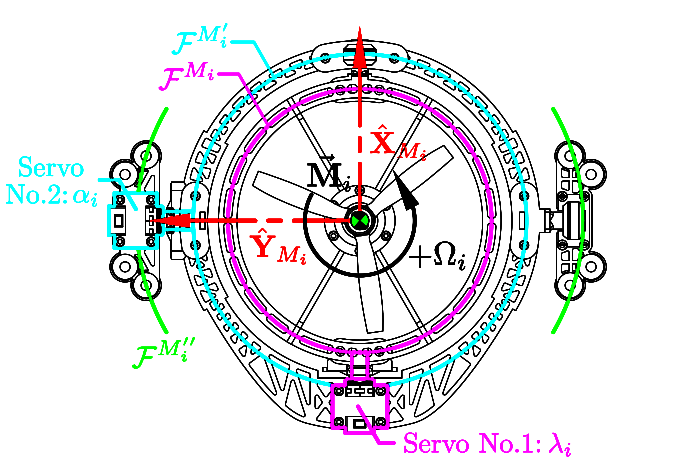
\includegraphics[width=0.9\textwidth]{figs/motor-frame}
\caption{Intermediate motor frames}
\label{fig:motor-frame}
\vspace{-8pt}
\end{figure}
\par
That inner ring frame rotates about its $\hat{X}_{M_i}$ axis by $\lambda_i$ from the module's first servo. The first servo is attached to the middle ring assembly with the frame $\mathcal{F}^{M_i'}$. The middle ring assembly, frame $\mathcal{F}^{M_i'}$, then rotates about its $\hat{Y}_{M_i'}$ axis actuated by the second $\alpha_i$ servo. That second servo is affixed to an intermediate $\mathcal{F}^{M_i''}$ frame, finally there's an orthogonal rotation about $\hat{Z}_{M_i''}$ between $\mathcal{F}^b$ and $\mathcal{F}^{M_i''}$. Each module's actuation state is fully described by the rotational speed, both servo positions and all their respective rates; $[\Omega_{i},~\lambda_{i},~\alpha_{i},~\dot{\Omega}_i,~\dot{\lambda}_i,~\dot{\alpha}_i]^{T}$ for $i\in [1:4]$. 
\par
Fig:\ref{fig:body-frame} shows how the axes of each motor module aligns with the body frame's axes at rest. The body frame $\mathcal{F}^b$ has the origin $\vec{\mathbf{O}}_b$ at the X-Y center of the structure, co-planar to each motor modules' center. \emph{Neither} the body frame's origin \emph{nor} each modules center of rotation are coincidental with body's center of mass. The exact disparity between the origin(s) of motion and the respective body's center of mass are quantified subsequently in Sec:\ref{sec:proto.inertia}. 
\begin{figure}[htbp]
\vspace{-6pt}
\centering
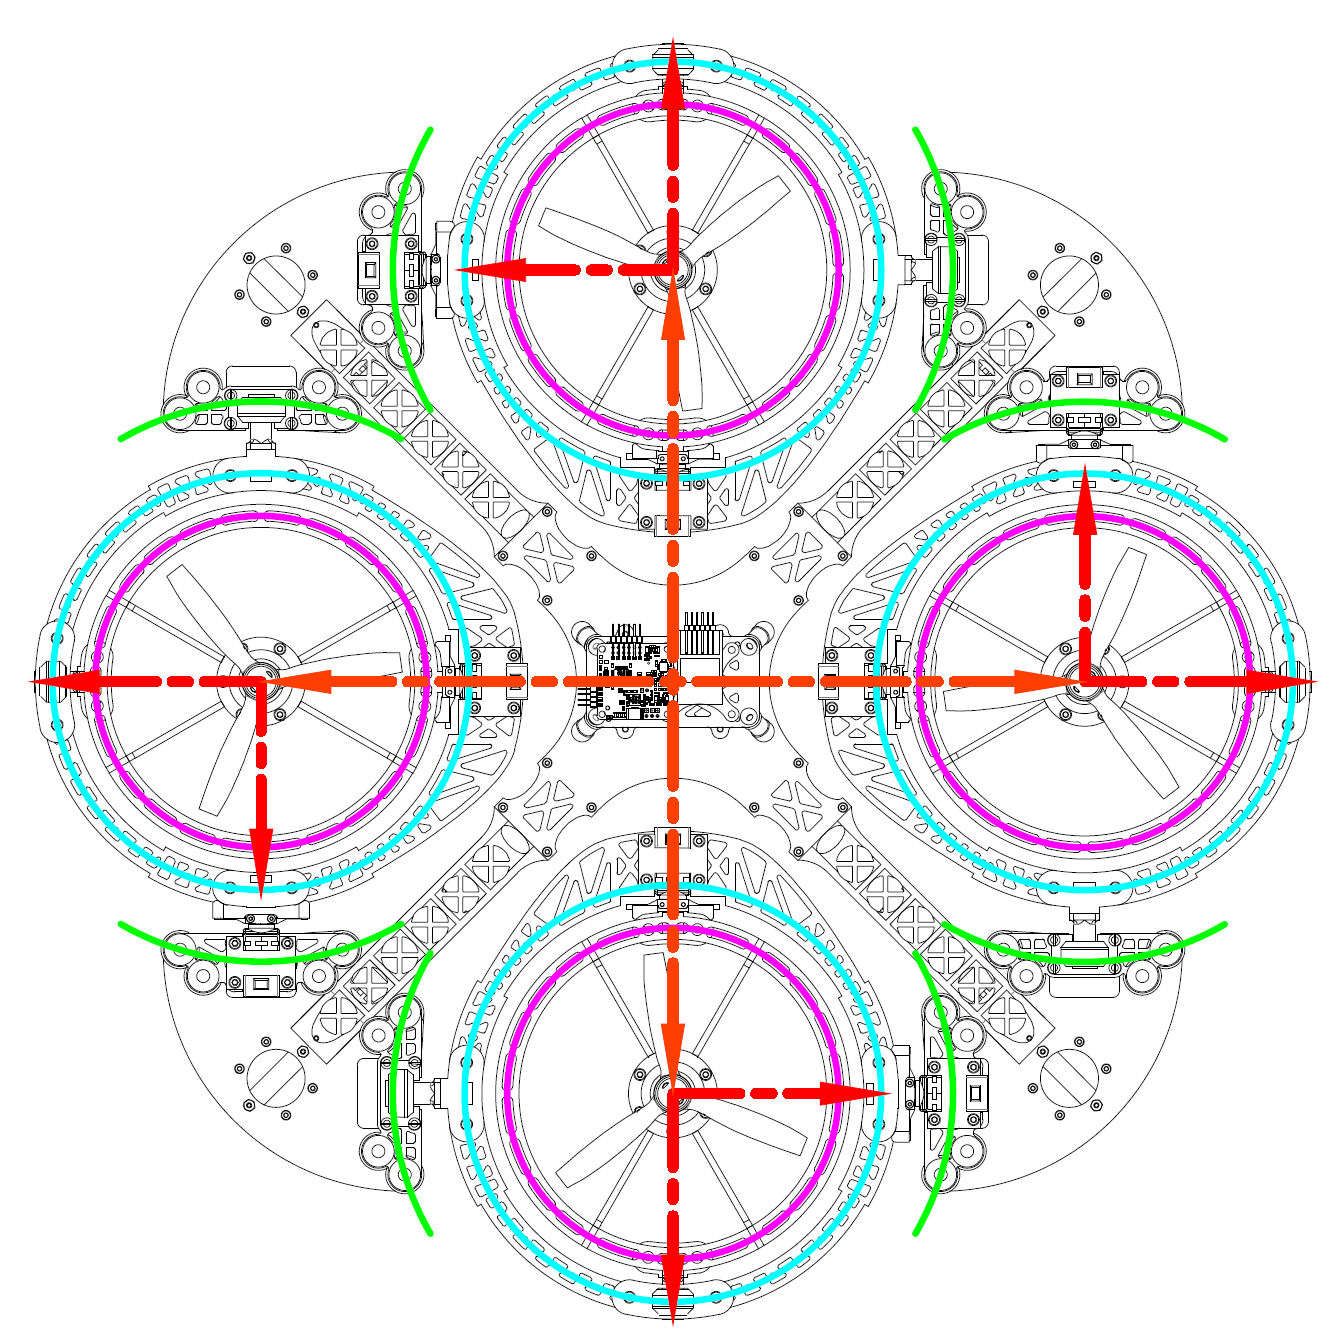
\includegraphics[width=0.85\textwidth]{figs/body-frame}
\vspace{-4pt}
\caption{Body frame axes layout}
\label{fig:body-frame}
\vspace{-16pt}
\end{figure}
\par
The motor module pair 1 and 3 have their $\hat{X}$-axes in the positive and negative $\hat{X}_b$ directions of the body frame respectively. Similarly Modules 2 and 4 have their $\hat{X}$-axes in the positive and negative $\hat{Y}_b$ directions of the body frame. Motor modules 1 and 3 have clockwise rotating propellers; denoted by a positive superscript or $\Omega_{[1,3]}^{+}$. Conversely modules 2 and 4 have counter-clockwise rotations; denoted by a negative superscript or $\Omega_{[2,4]}^{-}$.
\par
\emph{\color{Gray}Not shown in Fig:\ref{fig:body-frame} is the relative $\hat{Z}_b$ origin position of $\vec{\mathbf{O}}_b$ with respect to the entire assembly. The $\Delta Z$ height of the body's motion centroid is such that its origin is co-planar with the four motor modules rotational centers. The center of motion is \underline{not coincidental with the center of mass}.}
\par
\begin{figure}[htbp]
\centering
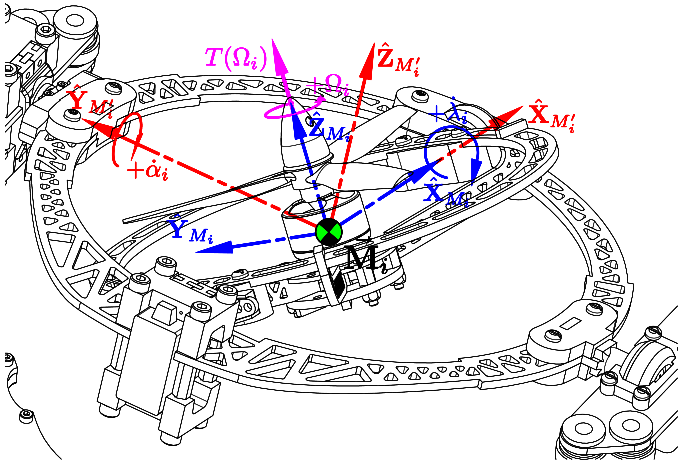
\includegraphics[width=0.75\textwidth]{figs/force-redirect}
\caption{Motor thrust force}
\label{fig:force-redirect}
\vspace{-16pt}
\end{figure}
Each motor is displaced from the body frame origin by the distance $L_{arm}=195.16~\text{mm}$ (shown in Fig:\ref{fig:body-frame}). Transformation of some vector $\vec{\nu}_{M_i}$ in the motor frame $\mathcal{F}^{M_i}$ to the body frame is given as three sequential rotation operations:
\begin{subequations}
\begin{equation}\label{eq:motor-module-rotation.a}
\vec{\nu}_b=R_{M_i}^b\vec{\nu}_{M_i}=R_z(-\sigma_i)R_y(-\alpha_i)R_x(-\lambda_i)\vec{\nu}_{M_i}~~~~\in\mathcal{F}^{b},~\text{for}~~\sigma_i\in\begin{bmatrix}
0 & \frac{\pi}{2} & \pi & \frac{2\pi}{3}
\end{bmatrix}
\end{equation}
The constant orthogonal $\sigma_i$ rotations about $\hat{Z}_{M_i''}$ are independent of actuator positions, $\sigma_i$ is determined by the motor module's location. The rotation matrices $R_z(\sigma_i)$ for $\sigma_i=(i-1)\pi/2$ are:
\begin{equation}\label{eq:motor-module-rotation.b}
R_z=\begin{bmatrix}
1 & 0 & 0\\
0 & 1 & 0\\
0 & 0 & 1
\end{bmatrix}, \begin{bmatrix}
0 & -1 & 0\\
1 & 0 & 0\\
0 & 0 & 1
\end{bmatrix}, \begin{bmatrix}
-1 & 0 & 0\\
0 & -1 & 0\\
0 & 0 & 1
\end{bmatrix}, \begin{bmatrix}
0 & 1 & 0\\
-1 & 0 & 0\\
0 & 0 & 1
\end{bmatrix}~\text{for}~i\in[1,2,3,4]~\text{respectively}
\end{equation}
\label{eq:motor-module-rotation}
\end{subequations}
If the propeller's rotation produces some thrust force $T(\Omega_i)$ in the motor module frame (Fig:\ref{fig:force-redirect}) which acts through the center of rotation $\vec{\mathbf{M}}_i$; that force is similarly transformed to the body frame through Eq:\ref{eq:motor-module-rotation.a}. A thrust vector for $\vec{T}_i\in\mathcal{F}^{M_i}$ in the body frame $\mathcal{F}^b$ is calculated:
\begin{equation}\label{eq:motor-module-force-redirect}
\vec{T}_i=R_z(-\sigma_i)R_y(-\alpha_i)R_x(-\lambda_i)\begin{bmatrix}0 & 0 & T(\Omega_i)\end{bmatrix}^T~~~~\in\mathcal{F}^{b}
\end{equation}
The actuator space, including propeller speed $\Omega_i$, is then $\in\mathbb{R}^{12}$, or rather $\mathbb{U}\in\mathbb{R}^{12}$, in contrast with $\mathbb{U}\in\mathbb{R}^4$ for a standard quadrotor. The actuator input set $u \in \mathbb{U}$ is then structured as:
\begin{equation}\label{eq:actuator-space}
\underset{\in\mathbb{U}}{u}=\begin{bmatrix}
\Omega_1^+ & \lambda_1 & \alpha_1 & \ldots & \Omega_4^- & \lambda_4 & \alpha_4
\end{bmatrix}^T~~~~\in\mathbb{R}^{12}
\end{equation}
\newpage
%====================================================
\section{Inertial Matrices \& Masses}
\label{sec:proto.inertia}
%====================================================
\emph{\color{Gray}When transforming inertias between reference frames it is more appropriate to use rotation matrices to apply the transformation and not quaternions. Spatial rotation of inertial matrices are ill suited to quaternion parametrization.}
\par
An undesirable consequence of relative rotations within a non-rigid body are the inertial responses associated with such movements. Given Newton's Second Law of Rotational Motion; each applied rotation is going to produce an equal but opposite reaction onto the principally inducing body. Similarly a gyroscopic cross-product from rotational velocities is also present when rotating bodies that have their own relative rotation. Typically for most rigid body dynamics (Sec:\ref{sec:dynamics.rigidbody}), such first and second order effects are negligible given that the angular rates on which they depend are small enough to approximate as zero; $\vec{\omega}_b\approx\vec{0}$. A dynamic setpoint (non-zero) attitude tracking plant is, however, going to produce time varying body angular velocities and accelerations that must be accounted for.
\par
The dynamic effects of those torque responses are derived later in Sec:\ref{subsec:dynamics.nonlinearities.gyrotorques}. Both inertial and gyroscopic effects are dependent on the considered body's rotational inertia about each respective axis. The magnitude of those inertias are ostensibly a by-product of the structure's design but also the vehicle's instantaneous configuration.
\par
The following inertias presented are all calculated from a SolidWorks model with masses to match physical measurements of the constructed prototype. Each connected body affected by the same angular velocity is grouped together. Every motor module then contains 3 independent inertial bodies; the propeller/rotor body, the inner ring and finally middle ring assemblies, each of which are now described in detail. 
\begin{figure}[hbtp]
\vspace{-6pt}
\centering
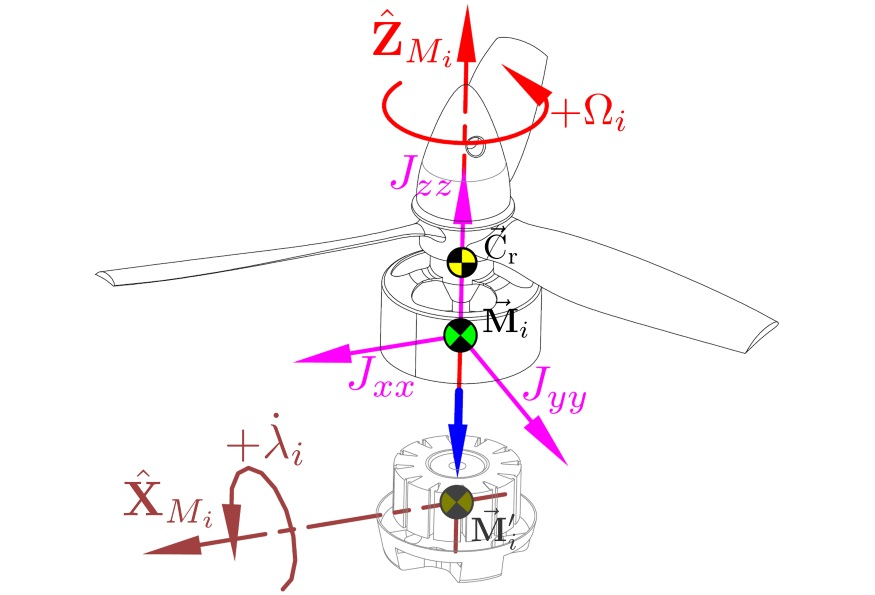
\includegraphics[width=0.71\textwidth]{figs/inertia-prop}
\caption{Rotor assembly rotational structure}
\label{fig:inertia-prop}
\vspace{-14pt}
\end{figure}
\par
The first rotational body to consider is that of the propeller and rotor assembly (Fig:\ref{fig:inertia-prop}, \underline{excluding} the motor's greyed out stator). The \emph{rotor} assembly, with subscript r, has a net mass $m_{\text{r}}=27~\text{g}$ with a center of mass $\text{C.M}_{\text{r}}=\begin{bmatrix}0.0&0.0&15.5\end{bmatrix}^T~\text{mm}$ relative to the entire motor modules center of rotation $\vec{\mathbf{M}}_i$. The propeller's rotation plane is similarly $\begin{bmatrix}0.0&0.0&23.0\end{bmatrix}^T~\text{mm}$ relative to $\vec{\mathbf{M}}_i$ (previously illustrated in Fig:\ref{fig:motor_prop}). 
\par
At high speeds the propeller's inertial contribution to the rotor assembly can be approximated as a solid disc. It follows that the inner ring's inertial components can then be regarded as constant with respect to $\Omega_i$; moreover its center of mass is independent of that propeller's rotation. 
\par
The entire rotor assembly then has a constant inertia $J_\text{r}$, with principle inertial axes centered and aligned as in Fig:\ref{fig:inertia-prop}:
\begin{equation}\label{eq:prop-inertia}
J_\text{r}=\begin{bmatrix}
105.5 & 0.0 & 0.0\\
0.0 & 105.5 & 0.0\\
0.0 & 0.0 & 41.8
\end{bmatrix}~~~~\text{g.cm}^2
\end{equation}
The net angular velocity of the rotor assembly, $\vec{\omega}_\text{r}$, relative to the body frame is produced by the BLDC motor's rotational velocity $\Omega_i$ and both servo rates; $\dot{\lambda}_i$ and $\dot{\alpha}_i$. Here $\Omega_i$ and both servo rates are measured in $\text{rad.s}^{\text{-}1}$, later $\Omega_i$ is needed in $\text{rev.s}^{\text{-}1}$ for Blade-element momentum theory thrust calculations (Sec:\ref{subsec:dynamics.aero.bem}). Each servo's angular velocity is \emph{transformed} onto the motor frame $\mathcal{F}^{M_i}$.
\begin{equation}\label{eq:net-angular-rot}
\vec{\omega}_\text{r}=\begin{bmatrix}
0\\
0\\
\Omega_i
\end{bmatrix}
+\frac{d\lambda_i}{dt}R_x(-\lambda_i)\begin{bmatrix}
\lambda_i\\
0\\
0
\end{bmatrix}+\frac{d\alpha_i}{dt}R_y(-\alpha_i)R_x(-\lambda_i)\begin{bmatrix}
0\\
\alpha_i\\
0
\end{bmatrix}~~~~\in\mathcal{F}^{M_i}
\end{equation}
\emph{\color{gray} Eq:\ref{eq:net-angular-rot} is later replaced with a quaternion operator. That equation and the remaining angular velocity equations for each body derived here are therefore not expanded further in their current rotation matrix form(s)\ldots}
\par
\begin{figure}[htbp]
\vspace{-12pt}
\centering
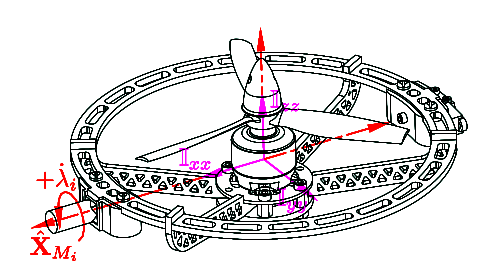
\includegraphics[width=0.75\textwidth]{figs/inertia-inner}
\vspace{-10pt}
\caption{Inner ring rotational structure}
\label{fig:inertia-inner}
\end{figure}
The next assembly, to which the motor frame $\mathcal{F}^{M_i}$ is attached, is the \emph{inner ring} assembly denoted with subscript n. The inner ring structure has a mass $m_\text{n}=92~\text{g}$, \underline{including} the rotor assembly in that calculation. The center of mass is positioned $\text{C.M}_{\text{n}}=\begin{bmatrix}-1.44&00.0&5.14\end{bmatrix}^T~\text{mm}$ relative to the module's center of rotation $\vec{\mathbf{M}}_i$. The inner ring, being rotated by the $\lambda_i$ servo about the $\hat{X}_{M_i}$ axis, then has an inertial matrix which \underline{includes} $J_r$ from Eq:\ref{eq:prop-inertia} centered and aligned with axes as in Fig:\ref{fig:inertia-inner}:
\begin{equation} \label{eq:inertia.inner}
J_\text{n}=J_{M_i}=\begin{bmatrix}
520.9 & -31.7	& -0.3\\
-31.7 & 1826.3 & 0.0\\
-0.3 & 0.0	& 2050.8\\
\end{bmatrix}~~~~\text{g.cm}^2
\end{equation}
The rotational velocity of the collective inner ring assembly $\vec{\omega}_\text{n}$, or $\vec{\omega}_{M_i}$ for the angular velocity of frame $\mathcal{F}^{M_i}$, is similar to that of Eq:\ref{eq:net-angular-rot}. They both occur in the same frame however the inner ring's angular velocity has no velocity contribution from $\Omega_i$:
\begin{equation}\label{eq:net-angular-inner}
\vec{\omega}_\text{n}=\vec{\omega}_{M_i/b}=\frac{d\lambda_i}{dt}R_x(-\lambda_i)\begin{bmatrix}
\lambda_i\\
0\\
0
\end{bmatrix}
+\frac{d\alpha_i}{dt}R_y(-\alpha_i)R_x(-\lambda_i)\begin{bmatrix}
0\\
\alpha_i\\
0
\end{bmatrix}~~~~\in\mathcal{F}^{M_i}
\end{equation}
\par
That first actuating servo for $\lambda_i$ and its coaxial support bearing are both affixed to the intermediate \emph{middle ring} assembly, with subscript m (middle ring only Fig:\ref{fig:inertia-middle}). The intermediate frame $\mathcal{F}^{M_i'}$ is attached to the middle ring body with a mass $m_\text{m}=98~\text{g}$, \underline{excluding} the inner most ring's contribution. That middle ring body alone has a center of mass $\text{C.M}_{\text{m}}=\begin{bmatrix}
-4.70&0.37&-0.36\end{bmatrix}^T~\text{cm}$ relative to $\vec{\mathbf{M}}_i$. 
\begin{figure}[htbp]
\centering
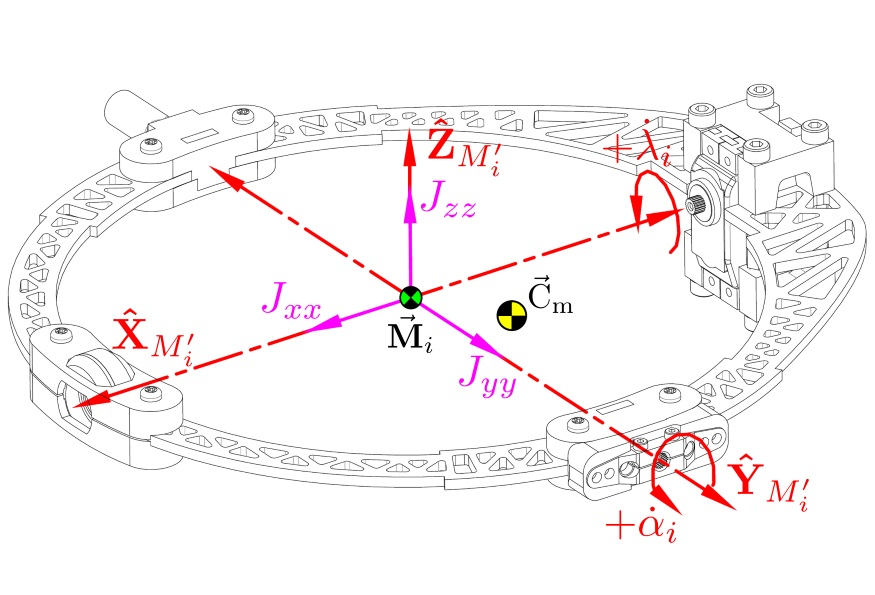
\includegraphics[width=0.7\textwidth]{figs/inertia-middle}
\vspace{-18pt}
\caption{Middle ring rotational structure}
\label{fig:inertia-middle}
\vspace{-12pt}
\end{figure}
\par
Together the inner and middle rings make the whole motor module assembly (Fig:\ref{fig:inertia-module}), with a subscript p. The net module has a mass $m_\text{p}=190~\text{g}$. The center of mass for the entire module, $\text{C.M}_\text{p}$,is a function of the inner ring's rotational position $\lambda_i$ relative to the middle frame $\mathcal{F}^{M_i'}$. That module's center of mass is calculated:
\begin{subequations}\label{eq:center-module}
\begin{equation}\label{eq:center-module.a}
\text{C.M}_{\text{n}}'=R_x(\lambda)\big(\text{C.M}_{\text{n}}\big)
\end{equation}
\vspace{-10pt}
\begin{equation}\label{eq:center-module.b}
\text{C.M}_\text{p}=\frac{m_\text{m}\big(\text{C.M}_{\text{m}}\big)+m_\text{n}\big(\text{C.M}_{\text{n}}'\big)}{m_\text{p}}
\end{equation}
Substituting physical values into Eq:\ref{eq:center-module.b} for the inner and middle rings' center of masses respectively:
\begin{equation}\label{eq:center-module.c}
\text{C.M}_\text{p}(\lambda)=\frac{98\begin{bmatrix}-4.70 & 0.37 & -0.36\end{bmatrix}^T\times 10^{-7}+92R_x(\lambda)\begin{bmatrix}
-1.44& 0.00 & 3.06
\end{bmatrix}^T\times 10^{-8}}{190\times 10^{-3}}
\end{equation}
Which then has a value at rest, for reference, with the servo $\lambda_i=0$ relative to the center of rotation $\vec{\mathbf{M}}_i$:
\begin{equation}\label{eq:center-module.d}
\text{C.M}_\text{p}(0)=	\begin{bmatrix}
-2.49 & 0.19 & 0.04
\end{bmatrix}^T\Big|_{\lambda_i=0}~~~~\text{cm}
\end{equation}
\end{subequations}
\par
%============================================ UP TO HERE ============================================
The complete motor module is rotated by the $\alpha_i$ servo about its $\hat{Y}_{M_i'}$ axis. The module's compound inertia $J_\text{p}$ is a combination of the middle ring's inertia $J_\text{m}$ and the inner ring's inertia $J_\text{n}$ rotated by $\lambda_i$ about $\hat{X}_{M_i}$ (aligned as per Fig:\ref{fig:inertia-module}). The latter's contribution is dependent on the \emph{rotation} (not transformation) angle $\lambda_i$ which from the conservation of angular momentum theory, detailed in \cite{rigidbodyinertia}, produces the net inertia of that frame; $J_{M_i'}$ or $J_\text{p}$:
\begin{subequations}\label{eq:inertia.middle}
\begin{equation} \label{eq:inertia.middle.a}
\text{With} ~~J_\text{m}=\begin{bmatrix}
2905.7 & 0.0 & 390.9\\
0.0 & 8446.4 & 0.0\\
390.9 & 0.0 & 11125.7\\
\end{bmatrix}~~~\text{g.cm}^2
\end{equation}
\vspace{-5pt}
\begin{equation}\label{eq:inertia.middle.b}
J_\text{p}(\lambda_i)=J_{M_i'}=J_\text{m}+R_{x}(\lambda_i)\big(J_\text{n}\big)R_{x}^{-1}(\lambda_i)
\end{equation}
Noting that $J_{M_i}=J_\text{n}$ is the inner ring's inertia from Eq:\ref{eq:inertia.inner}, but re-orientated through a rotation $R_x(\lambda_i)$. That inertia with $\lambda_i=0$ and relative to the middle ring frame $\mathcal{F}^{M_i'}$ has a reference value:
\begin{equation}
J_\text{p}(0)=\begin{bmatrix}
3365.4 & -0.1 & 390.6\\
-0.1 & 10210.1 & 0.0\\
390.6 & 0.0 & 13118.0             
\end{bmatrix}\Bigg|_{\lambda_i=0}~~~~[\text{g.cm}^2]
\end{equation}
Because $R_x$ is a full rank square matrix its inverse $R^{-1}_{x}$, used in Eq:\ref{eq:inertia.middle.b}, always exists. The module's inertia could be further divided into constant and variable components; $J_\text{p}(\lambda_i)=J_{const}+J_{M_i}(\lambda_i)$. The variable terms can, under certain conditions, be simplified and neglected\ldots
\par
\begin{figure}[htbp]
\vspace{-10pt}
\centering
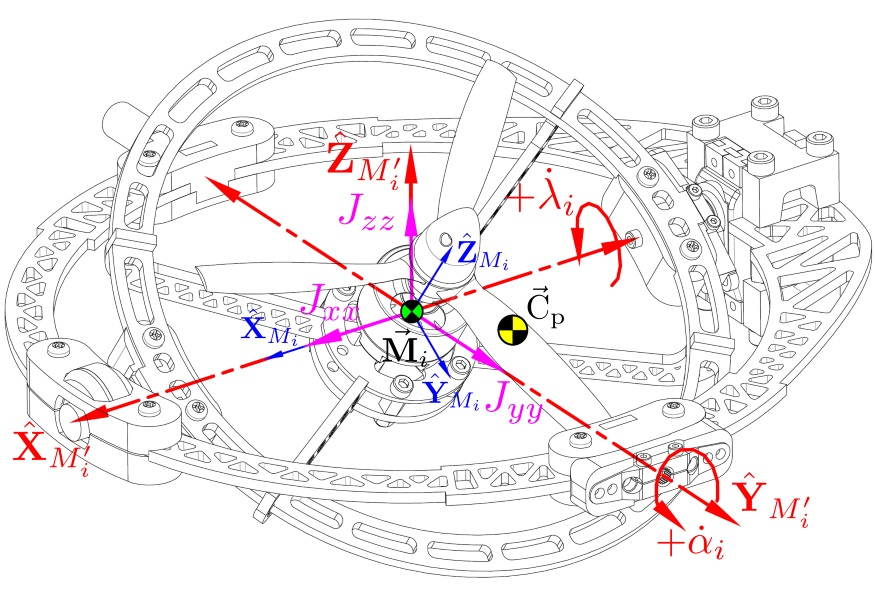
\includegraphics[width=0.7\textwidth]{figs/inertia-module}
\caption{Module assembly rotational structure}
\vspace{-8pt}
\label{fig:inertia-module}
\end{figure}
Fig:\ref{fig:inertia-damping} shows how the complete motor module and its rotational axes (in Fig:\ref{fig:inertia-module}) are attached and centered relative to the body structure. The second $\alpha_i$ servo is affixed to the body structure and rotates the entire motor module.
\begin{figure}[hbtp]
\centering
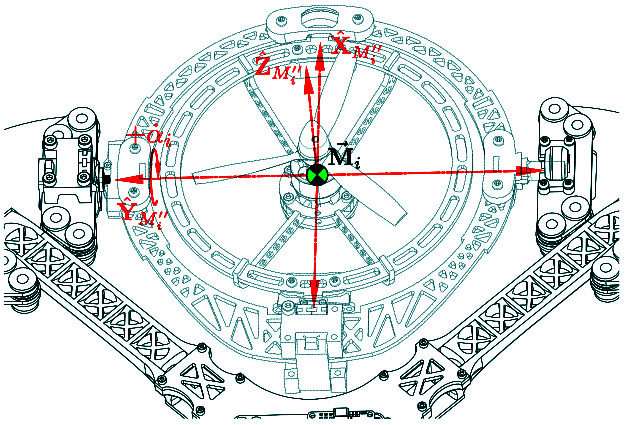
\includegraphics[width=0.85\textwidth]{figs/inertia-damping}
\caption{Complete motor module attached to the body structure}
\label{fig:inertia-damping}
\vspace{-14pt}
\end{figure}
\par
Finally, the angular velocity experienced by the net motor assembly relative to the body frame, $\vec{\omega}_\text{p}$ in frame $\mathcal{F}^{M_i'}$, is entirely as a result of the $\alpha_i$ servo actuation:
\begin{equation}
\vec{\omega}_\text{p}=\vec{\omega}_{M_i'/b}=\frac{d\alpha_i}{dt}R_y(-\alpha_i)\begin{bmatrix}
0\\
\alpha_i\\
0
\end{bmatrix}~~~~\in\mathcal{F}^{M_i'}
\end{equation}
\end{subequations}
That $\alpha_i$ servo is affixed to the body structure and so its inertial volume and that of the outer coaxial bearing support contributes then to the body structure's inertia; whose value excludes any of the four motor modules. Attached to that servo is an intermediate frame $\mathcal{F}^{M_i''}$ (Fig:\ref{fig:inertia-damping}) which differs from the middle ring frame by an $R_y(-\alpha_i)$ transformation and differs from the body frame $F^b$ by an orthogonal $R_z(\sigma_i)$ rotation.
\par
The motor modules are suspended from the body frame with a set of silicone damping balls. The \emph{body structure} which includes those connecting masses, with a subscript y, has center of mass $\text{C.M}_{\text{y}}$ (without any motor modules attached, Fig:\ref{fig:inertia-center}). The center of mass coincides with the $\hat{X}_b$ and $\hat{Y}_b$ directional axes but lies $\Delta Z=-9.52~[\text{mm}]$ below the body frame's origin of motion $\vec{\mathbf{O}}_b\in\mathcal{F}^b$.
\par
\begin{figure}[hbtp]
\centering
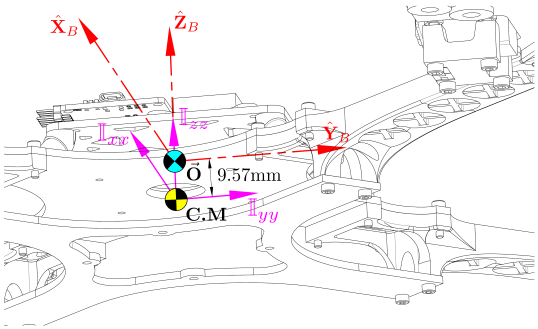
\includegraphics[width=0.81\textwidth]{figs/inertia-center}
\caption{Body structure's center of mass}
\label{fig:inertia-center}
\vspace{-6pt}
\end{figure}
\par
\emph{\color{Gray}Note: that body frame origin $\vec{\mathbf{O}}_b$ which all motion is calculated with respect to is co-planar to the motor module's rotational centers, \underline{not the net center of mass}.}
\par
The body structure's weight, including all four damping assemblies and electronics, totals to $m_\text{y}=814.70~[\text{g}]$. Similarly the body structure's net inertia (\emph{sans} motor modules) $J_\text{y}$, about its center of mass (Fig:\ref{fig:inertia-center}), is:
\begin{subequations}\label{eq:inertia.body}
\begin{equation}\label{eq:inertia.body.a}
\underset{C.M}{J_\text{y}}=\begin{bmatrix}
181569.7 & 0.4 &-19.4\\
0.4 & 181692.2 & 8.9\\
-19.4 & 8.8 & 360067.2\\
\end{bmatrix}\times 10^{-7}~~~[\text{kg.m}^2]
\end{equation}
Using the Parallel Axis theorem to translate that inertia to the origin of motion by $\Delta Z=+9.52~[\text{mm}]$, the inertia about the origin, $\vec{\mathbf{O}}_b$, is:
\begin{equation}\label{eq:inertia.body.b}
J'=J+m\big(\vec{d}\cdot\vec{d}-\vec{d}\otimes\vec{d}\hspace{3pt}\big)\approx J+md^2
\end{equation}
\emph{\color{Gray}For the general parallel axis transformation in Eq:\ref{eq:inertia.body.b}, $\otimes$ represents the Hamilton product of two $[3\times 1]$ matrices. It is used later to indicate quaternion multiplication. The vector $\vec{d}$ is the difference between the center of mass $\mathbf{C.M}_\text{y}$ and the body frame origin $\vec{\mathbf{O}}_b$.}
\begin{equation}
\therefore J_y'=\underset{C.M}{J_\text{y}}+m_\text{y}\big(\Delta\vec{Z}\cdot\Delta\vec{Z}-\Delta\vec{Z}\otimes\Delta\vec{Z}\big)
\end{equation}
That body's constant inertia $J_\text{y}$ at the origin $\vec{\mathbf{O}}_b$ and aligned with the body frame $\mathcal{F}^{b}$ is then:
\begin{equation}\label{eq:inertia.body.c}
\rightarrow\underset{\vec{\mathbf{O}}_b}{J_\text{y}'}=\begin{bmatrix}
182307.7 & 0.4 & -14.5\\
0.4 & 182430.1 & 6.5\\
-14.5& 6.5 & 360067.2
\end{bmatrix} \times10^{-7}~~~[\text{kg.m}^2]
\end{equation}
\end{subequations}
Net inertia for the complete multibody vehicle, $J_b(u)$ about the origin $\vec{\mathbf{O}}_b$, is a combination of all the relative attached bodies as a function of all actuator positions $u\in\mathbb{U}$. The entire assembly's inertia $J_b(u)$ is the \emph{net} body frame's inertia, different from $J_\text{y}$ which is the inertia for \emph{only} the body structure. That collective assembly being the four motor modules, each rotated first by $\lambda_i$, then $\alpha_i$ and finally translated to the body frame origin; and the body structure's contribution itself. 
\par
Those motor modules' inertial transformations from their respective centers of rotation, in frames $\mathcal{F}^{M_i}$ for $i\in[1:4]$, to the body frame $\mathcal{F}^b$ are analogous to that of Eq:\ref{eq:motor-module-rotation}. Reiterating that $\vec{\mathbf{O}}_b$ is \emph{co-planar} to each module's center of rotation; each motor module's inertia, $J_\text{p}(\lambda_i)$ or $J_{M_i'}$, defined in Eq:\ref{eq:inertia.middle.b}, is further rotated by $\alpha_{i}$ about the $\hat{Y}_{M_i'}$ axis and finally an orthogonal $\hat{Z}_{M_i''}$  axis rotation (aligned with $\hat{Z}_b$) onto $\mathcal{F}^b$. 
\par
\begin{figure}[hbtp]
\vspace{-6pt}
\centering
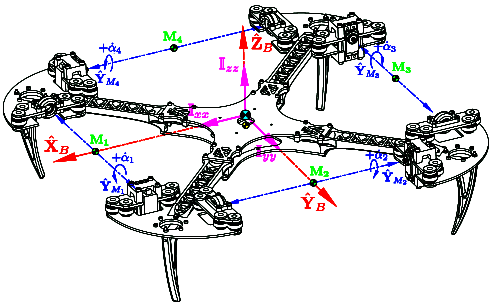
\includegraphics[width=\textwidth]{figs/inertia-frame}
\caption{Inertial, mass and motor modules respective centers}
\label{fig:inertia-frame}
\vspace{-6pt}
\end{figure}
For the entire body's net inertia each contributing assembly's inertia must be defined with respect to the body's origin; first aligned parallel to the common set of body frame axes $\hat{X}_b,\hat{Y}_b$ and $\hat{Z}_b$ and then translated to the origin $\vec{\mathbf{O}}_b$. Each motor module's inertia, still centered relative to each individual rotational centers $\vec{\mathbf{M}}_i$ in Fig:\ref{fig:inertia-frame}, but re-orientated to align parallel with $\vec{\mathbf{O}}_b$ with rotations about axes $\hat{X}\in\mathcal{F}^{M_i},~\hat{Y}\in\mathcal{F}^{M_i'},~\hat{Z}\in\mathcal{F}^{M_i''}$, is calculated:
\begin{subequations}\label{eq:module-inertia}
\begin{equation}\label{eq:module-inertia.a}
J_{\vec{\mathbf{M}}_i}(u\cdot i)=R_{z}(\sigma_i)R_{y}(\alpha_i)\big(J_{p}(\lambda_i)\big)R^{-1}_{y}(\alpha_i)R^{-1}_{z}(\sigma_i)~\text{for}~i\in[1:4]
\end{equation}
The argument $(u\cdot i)$ in Eq:\ref{eq:module-inertia.a} is the i\textsuperscript{th} projection of the actuator space; that being $\begin{bmatrix}\Omega_i&\lambda_i&\alpha_i\end{bmatrix}^T$.
Furthermore the rotation $R_{z}(\sigma_i)$ was defined as an orthogonal $\hat{Z}_b$ rotation previously in Eq:\ref{eq:motor-module-rotation.b}. Expanding each module's inertia to individual inner and middle ring inertial contributions then yields:
\begin{equation}\label{eq:module-inertia.c}
\therefore J_{\vec{\mathbf{M}}_i}(u\cdot i)=R_{z}R_{y}(\alpha_i)\big(J_\text{m}\big)R^{-1}_{y}(\alpha_i)R^{-1}_z+R_{z}R_{y}(\alpha_i)R_{x}(\lambda_i)\big(J_\text{n}\big)R^{-1}_{x}(\lambda_i)R^{-1}_{y}(\alpha_i)R^{-1}_z
\end{equation}
\end{subequations}
\emph{\color{Gray}It's at this stage that, despite simplifications, the symbolic inertial equations all become overly cumbersome to include with numeric values\ldots~For the sake of brevity, exact calculated inertial values for the input dependent plant are omitted.}
\par
Each module's rotational center, vectors $\vec{\mathbf{M}}_{1\rightarrow 4}$, are all equally spaced relative to the origin of motion, $\vec{\mathbf{O}}_b$, with a parallel axis arm $L_{arm}=195.16~~[\text{mm}]$ (Fig:\ref{fig:inertia-frame}). To avoid notational confusion the term $\vec{L}_i=\begin{bmatrix} \pm 195.16 & 0 & 0 \end{bmatrix}^T$ or $\begin{bmatrix} 0 & \pm 195.16 & 0
\end{bmatrix}^T$ is used to represent the vector displacement between the origin $\vec{\mathbf{O}}_b$ and each motor modules center of rotation $\vec{\mathbf{M}}_{1\rightarrow 4}$. The net inertial equation $J_b(u)$, about the origin $\vec{\mathbf{O}}_b$ and depending on the actuator position matrix $u\in\mathbb{U}$, can be calculated as:
\begin{subequations}
\label{eq:body-inertia}
\begin{equation}\label{eq:body-inertia.a}
\underset{\vec{\mathbf{O}}_b}{J_b(u)}=J_\text{y}+\sum_{i=1}^{4}J'_{\vec{\mathbf{M}}_i}(u\cdot i)~~~~[\text{kg.m}^2],~u\in\mathbb{U}
\end{equation}
Where $J'_{\vec{\mathbf{M}}_i}(u\cdot i)$ is the motor module inertia from Eq:\ref{eq:module-inertia} but translated to the origin $\vec{\mathbf{O}}_b$ using a parallel axis theorem with $m_\text{p}=190~[\text{g}]$:
\begin{equation}\label{eq:body-inertia.b}
J'_{\vec{\mathbf{M}}_i}(u\cdot i)=J_{\vec{\mathbf{M}}_i}(u\cdot i)+m_\text{p}\big(\vec{L}_i \cdot \vec{L}_i - \vec{L}_i\otimes\vec{L}_i\big)
\end{equation}
\end{subequations}
Although Eq:\ref{eq:body-inertia} produces the net multi-body's inertia, each equation to calculate $J_{\vec{\mathbf{M}}_i}'$ involves cascaded transformations which may deteriorate the results certainty. Each module's inertia is first translated to their respective centers of rotation then rotated as per the two servos and then finally translated again back to the body frame's origin. 
\par
Alternatively the inertia contribution of each sub-assembly can be considered separately and translated directly to the body frame's origin from their respective mass centers. This will improve the accuracy of the produced inertial equations, each translation/rotation has with it an associated floating point concatenation. It is also perhaps more intuitive for the reader to consider each sub-body's contribution individually, despite having been derived as combined inertial bodies in the above. The vehicles net inertia can then be described as nine separate contributing bodies; four inner rings $J_\text{n}$, four middle rings $J_\text{m}$ and one body structure $J_\text{y}$:
\begin{equation}\label{eq:body-net}
\underset{\vec{\mathbf{O}}_b}{J_b(u)}=\underset{\vec{\mathbf{O}}_b}{J'_\text{y}}+\sum_{i=1}^{4} \underset{\vec{\mathbf{O}}_b}{J_\text{n}}(u\cdot i)+\sum_{i=1}^{4} \underset{\vec{\mathbf{O}}_b}{J_\text{m}}(u\cdot i)~~~~u\in\mathbb{U}
\end{equation}
Isolating each body and considering each inertia independently; starting with the inner ring's, having an inertia $J_\text{n}$ with respect to its \emph{center of mass} (and not center of rotation) measured \emph{relative} to its center of rotation. The following is then fundamentally different from the process in Eq:\ref{eq:inertia.inner}, calculating the inner ring's inertial contribution about the origin $\vec{\mathbf{O}}_b$.
\par
%==========================================================
\begin{subequations}
\label{eq:body-net-inner}
For the inner ring only, with a mass $m_\text{n}$ and center of mass $C.M_\text{n}$ relative to its center of rotation $\vec{\mathbf{M}}_i$. The inner ring(s) contribution then follows:
\begin{equation}\label{eq:body-net-inner.a}
m_\text{n}=92~~[\text{g}]
\end{equation}
\vspace{-10pt}
\begin{equation}\label{eq:body-net-inner.b}
C.M_\text{n}=\begin{bmatrix}
-1.44 & 0.0 & 5.14
\end{bmatrix}^T~~~~[\text{mm}],~\in\mathcal{F}^{M_i}
\end{equation}
The inner ring's inertial matrix about it's center of mass (Fig:\ref{fig:inertia-inner}) is the constant:
\begin{equation}\label{eq:body-net-inner.c}
\underset{C.M}{J_\text{n}}=\begin{bmatrix}
496.6 & -31.7 & 6.6\\
-31.7 & 1800.1 & 0.0\\
6.6 & 0 & 2048.9
\end{bmatrix}~~~~[\text{g.cm}^2]
\end{equation}
Relative to the body frame's origin $\vec{\mathbf{O}}_b$ the inner ring has a center of mass, rotated by $\lambda_i$ and $\alpha_i$ servos about their respective axes with a relative orthogonal $R_z$ rotation too, is then:
\begin{equation}\label{eq:body-net-inner.d}
C.M'''_\text{n}=R_zR_y(\alpha_i)R_x(\lambda_i) \big(C.M_\text{n}\big)~~~~\in\mathcal{F}^{b}
\end{equation}
So transforming the inertia from Eq:\ref{eq:body-net-inner.c}, still about the center of mass $C.M_\text{n}'''$, but with axes aligned parallel with the body frame, or using the shorthand $||\vec{\mathbf{O}}_b$. The inner ring's inertia as a function of both servo angles $\lambda_i$ and $\alpha_i$ is:
\begin{equation}\label{eq:body-net-inner.e}
\underset{||\vec{\mathbf{O}}_b}{J'''_\text{n}(\lambda_i,\alpha_i)}=R_zR_y(\alpha_i)R_x(\lambda_i)\big(J_\text{n}\big)R^{-1}_x(\lambda_i)R^{-1}_y(\alpha_i)R^{-1}_z
\end{equation}
The vector difference between the new, rotated center of mass $C.M_\text{n}'''$ with the body origin $\vec{\mathbf{O}}_b$ is given by:
\begin{equation}
\Delta L = \vec{L}_i-C.M'''_\text{n}
\end{equation}
Then using the above with a parallel axis translation, adapted from Eq:\ref{eq:inertia.body.b}, to move the rotated inertia $J'''_\text{n}$ to the center of the body frame $\vec{\mathbf{O}}_b$:
\begin{equation}
\underset{\vec{\mathbf{O}}_b}{J_\text{n}}=\underset{||\vec{\mathbf{O}}_b}{J'''_\text{n}}+ m_\text{n} \big((\Delta L \cdot \Delta L)\mathbb{I}_{3\times 3} - \Delta L \otimes \Delta L \big)
\end{equation}
And for reference when both servos are at rest; $\lambda_i=0$ and $\alpha_i=0$, the inner ring's inertial contribution about the origin is explicitly:
\begin{equation}
\underset{\vec{\mathbf{O}}_b}{J_\text{n}}=\begin{bmatrix}
520.9 & -31.0 & 922.6\\
-31.0 & 36348.5 & 0.0\\
922.6 & 0.0 & 36573.0
\end{bmatrix}\times 10^{-7}\bigg|_{\lambda_i,\alpha_i=0}~~~~[\text{kg.m}^2],~\in\mathcal{F}^{b}
\end{equation}
\end{subequations}
Similarly, the same process is applied for the middle ring's rotated and translated inertia. The middle ring \emph{only} (Fig:\ref{fig:inertia-middle}) has a mass and center of mass relative to the module's center of rotation respectively:
\begin{subequations}
\label{eq:body-net-middle}
\begin{equation}\label{eq:body-net-middle.a}
m_\text{m}=98~~[\text{g}]
\end{equation}
\vspace{-14pt}
\begin{equation}
C.M_\text{m}=\begin{bmatrix}
-47.00 & 3.74 & -3.63
\end{bmatrix}^T~~~~[\text{mm}],~\in\mathcal{F}^{M_i'}
\end{equation}
The inertial matrix of the middle ring body, excluding the inner ring, about its center of mass is:
\begin{equation}
\underset{C.M}{J_\text{m}}=\begin{bmatrix}
2879.1 & 172.3 & 223.6\\
172.3 & 6269.0 & 13.3\\
223.6 & 13.3 & 8947.5\\
\end{bmatrix}~~~~[\text{g.cm}^2]
\end{equation}
Rotating the center of mass only by the $\alpha_i$ servo about the $\hat{Y}_{M_i'}$ axis yields the center of mass $C.M_\text{m}'$ relative to $\vec{\mathbf{O}}_b$:
\begin{equation}\label{eq:body-net-middle.d}
C.M''_\text{m}=R_{z}R_{y}(\alpha_i)\big(C.M_\text{m}\big)~~~~\in\mathcal{F}^{b}
\end{equation}
Then the rotated inertial matrix, aligned with axes parallel to the body frame origin $\vec{\mathbf{O}}_b$, follows:
\begin{equation}
\underset{||\vec{\mathbf{O}}_b}{J''_\text{m}}=R_zR_y(\alpha_i)\big(J_\text{m}\big)R^{-1}_y(\alpha_i)R^{-1}_z
\end{equation}
The vector difference from the rotated center of mass to the body frame origin is calculated:
\begin{equation}
\Delta L = \vec{L}_i-{C.M''_\text{m}}
\end{equation}
Which then leads to the parallel axis translation of the middle ring's inertia to the body origin:
\begin{equation}
\underset{\vec{\mathbf{O}}_b}{J_\text{m}}=\underset{||\vec{\mathbf{O}}_b}{J''_\text{m}}+m_\text{m}\big((\Delta L\cdot\Delta L)\mathbb{I}_{3x3}-\Delta L \otimes \Delta L \big)
\end{equation}
Again for reference; at rest with the middle ring servo $\alpha_i=0$ the middle ring's inertial contribution at $\vec{\mathbf{O}}_b$ is:
\begin{equation}
\underset{\vec{\mathbf{O}}_b}{J_\text{m}}=\begin{bmatrix}
2905.7 & 715.4 & -303.9\\
715.4 & 27795.7 & 0.0\\
-303.9 & 0.0 & 30475.0
\end{bmatrix}
\times 10^{-7}\Big|_{\alpha_i=0}~~~~[\text{kg.m}^2],~\in\mathcal{F}^{b}
\end{equation}
\end{subequations}
Then, reiterating Eq:\ref{eq:body-net}, the instantaneous inertia of the entire body in motion is calculated as the contribution of the connected sub-bodies depending on the actuator matrix $u\in\mathbb{U}$.
\begin{subequations}
\begin{equation}\label{eq:body-net-2}
\underset{\vec{\mathbf{O}}_b}{J_b(u)}=\underset{\vec{\mathbf{O}}_b}{J'_\text{y}}+\sum_{i=1}^{4} \underset{\vec{\mathbf{O}}_b}{J_\text{n}(u\cdot i)}+\sum_{i=1}^{4} \underset{\vec{\mathbf{O}}_b}{J_\text{m}(u\cdot i)}~~~~u\in\mathbb{U}
\end{equation}
The mass for the whole vehicle is $m_b=1574.7~[\text{g}]$. For reference and using Eq:\ref{eq:body-net-2}; the inertial matrix for the assembly at the actuator rest conditions, $u=\vec{0}$, about the origin $\vec{\mathbf{O}}_b$ is:
\begin{equation}
J_b(\vec{0})=\begin{bmatrix}
317448.2 & 0.4 & -14.5\\
0.4 & 317570.7 & 6.5\\
-14.5 & 6.5 & 628257.5
\end{bmatrix}\times 10^{-7}\bigg|_{u=\vec{0}}~~~~[\text{kg.m}^2],~\in\mathcal{F}^b
\end{equation}
\end{subequations}
The maximal variation of the body's net inertia is determined by the maximum determinant of the inertial matrix in Eq:\ref{eq:body-net-2} for some actuator state $max(det|J_b(u_\Lambda)|)~,u_\Lambda\in\mathbb{U})$. A maximum $J_b(u_\Lambda)$, with a determinant $det|J_b(u_\Lambda)|=1017.93\times 10^{-7}$, is:
\begin{subequations}\label{eq:inertia-max}
\begin{equation}
J_b(u_\Lambda)=\begin{bmatrix}
384695.4 & 0.4 & -14.5\\
0.4 & 384717.9 & 6.5\\
-14.5 & 6.5 & 687970.7
\end{bmatrix}\times 10^{-7}\bigg|_{u_\Lambda}~~~~[\text{kg.m}^2],~\in\mathcal{F}^b
\end{equation}
With an actuator matrix, independent of propeller speeds $\Omega_{1\rightarrow 4}$, as follows:
\begin{equation}
u_\Lambda=\begin{bmatrix*}[l]
\Omega_1, & \lambda_1=178\text{\textdegree},&\alpha_1=260\text{\textdegree}\ldots\\
\Omega_2, & \lambda_2=178\text{\textdegree},&\alpha_2=260\text{\textdegree}\ldots\\
\Omega_3, & \lambda_3=178\text{\textdegree},&\alpha_3=~~~0\text{\textdegree}\ldots\\
\Omega_4, & \lambda_4=~~~0\text{\textdegree}, & \alpha_4=~~~0\text{\textdegree}
\end{bmatrix*}
\end{equation}
\end{subequations}
Conversely, the minimum net inertia for the body is determined from the smallest determinant of Eq:\ref{eq:body-net-2}, for the actuator state $min(det|J_b(u_\Upsilon)|),~u_\Upsilon\in\mathbb{U}$. A minimum $J_b(u_\Upsilon)$, with a determinant $det|J_b(u_\Upsilon)|=633.48\times 10^{-7}$, is:
\begin{subequations}\label{eq:inertia-min}
\begin{equation}
J_b(u_\Upsilon)=\begin{bmatrix}
317469.0 & 0.4 & -1219.0\\
0.4 & 317591.5 & 1195.3\\
-1219.0 & 1195.3 & 628298.1
\end{bmatrix}\times 10^{-7}\bigg|_{u_\Upsilon}~~~~[\text{kg.m}^2],~\in\mathcal{F}^b
\end{equation}
When an actuator matrix for that minimum inertia is:
\begin{equation}
u_\Upsilon=\begin{bmatrix*}[l]
\Omega_1, & \lambda_1=178\text{\textdegree},&\alpha_1=~~~0\text{\textdegree}\ldots\\
\Omega_2, & \lambda_2=~~~0\text{\textdegree},&\alpha_2=260\text{\textdegree}\ldots\\
\Omega_3, & \lambda_3=~~~0\text{\textdegree},&\alpha_3=~~~0\text{\textdegree}\ldots\\
\Omega_4, & \lambda_4=~~~0\text{\textdegree}, & \alpha_4=~~~0\text{\textdegree}
\end{bmatrix*}
\end{equation}
\end{subequations}
The inclusion of Eq:\ref{eq:inertia-max} and Eq:\ref{eq:inertia-min} is used for maximum and minimum Eigen values of the body's inertial matrix at a later stage in the control derivation, Sec:\ref{sec:control.attitude}. It is interesting to note that both extremes of $J_b(u)$ are still symmetrical, and \emph{roughly} diagonal. Actuator positions hardly affect the skew products of inertia in $J_b(u)$ but can vary the diagonal moments of inertia by almost $20\%$ of their principle value.
\par
Unless otherwise specified; any inertia $J_b(u)$ indicates an instantaneous calculated solution to Eq:\ref{eq:body-net-2} given a particular $u(t)\in\mathbb{U}$. The purpose of the derivations for rotated centers of mass in Eq:\ref{eq:body-net-inner} and Eq:\ref{eq:body-net-middle} is twofold; highlighting both the inertial contributions \emph{and} the variable center of masses for each sub-body. Seeing that the origin of motion $\vec{\mathbf{O}}_b$ in the body frame $\mathcal{F}^b$ and the body's effective center of mass $C.M_\text{b}$ are not coincidental, it is important to quantify the net center of mass's variation with actuator positions $u\in\mathbb{U}$. 
\par
In the general case for a collection of $n$ bodies, with each body's center of mass at some position $\vec{X}_i$ and each having a mass $m_i$, resultant center of mass is:
\begin{subequations}\label{eq:mass-center}
\begin{equation}\label{eq:mass-center.a}
C.M = \frac{\sum_{i=1}^{n} m_i.\vec{X}_i}{\sum_{i=1}^{n} m_i}
\end{equation}
Using $C.M_\text{n}'''$ and $C.M_\text{m}''$ as rotated centers of mass defined in Eq:\ref{eq:body-net-inner.d} and Eq:\ref{eq:body-net-middle.d} respectively and $C.M_\text{y}$ for the body structure, the vehicle has a variable center of mass $C.M_\text{b}(u)$:
\begin{equation}\label{eq:mass-center.b}
C.M_\text{b}(u)=\frac{m_\text{y}C.M_\text{y}+\sum_{i=1}^{4} m_\text{n}C.M_\text{n}'''(u\cdot i)+\sum_{i=1}^{4} m_\text{m}C.M_\text{m}''(u\cdot i)}{m_\text{b}}
\end{equation}
\end{subequations}
So the net center of gravity when all actuators are at their zero positions is: $C.M_b(\vec{0})=\begin{bmatrix}0 & 0 & -4.94\end{bmatrix}^T~[\text{mm}]$. Using a gravity force vector $\vec{G}_b$ in the body frame as a result of gravitational acceleration $g=-9.81~[\text{m.s}^{\text{-}2}]$ acting on the vehicle:
\begin{subequations}\label{eq:grav-def}
\begin{equation}
\vec{G}_b=R_I\big(\vec{\eta}\big)^b\vec{G}_I~~~~[\text{N}],~\in\mathcal{F}^b
\end{equation}
\vspace{-14pt}
\begin{equation}
=R_I^b\big(\vec{\eta}\big)\begin{bmatrix}0&0&-9.81(m_\text{b})\end{bmatrix}^T
\end{equation}
The resultant gravitational torque about the origin $\vec{\mathbf{O}}_b$ in the body frame $\mathcal{F}^b$ from the varying eccentric center of mass for the vehicle is:
\begin{equation}
\Delta C.G = \vec{\mathbf{O}}_b-C.M_\text{b}(u)
\end{equation}
\vspace{-15pt}
\begin{equation}\label{eq:grav-torque}
\vec{\tau}_g=\Delta C.G\times m_b\vec{G}_b~~~~[\text{N.m}],\tau_g\in\mathcal{F}^b
\end{equation}
\end{subequations}
Uncertainty with inertial measurements, proven to be destabilizing and detrimental to control efforts in \cite{inertiafree,inertiaspin}, can indeed be incorporated into state dependent plant uncertainty  compenstaion like in \cite{intelligentbackstep}. Controllers with strong disturbance and uncertainty rejection, like a well designed $\text{H}_\infty$ controller, would be ideally suited to controlling an attitude plant without having to explicitly specify all of the above inertias. 
\par
It is, however, worth the mathematical deliberation to detail each inertial equation given that Lagrange dynamics are later applied to determine the servo actuator dynamic responses (Sec:\ref{sec:dynamics.nonlinearities}). Such equations of motion will later need explicit terms defined for instantaneous transformed inertias.
\newpage
%====================================================
\section{Electronics}
\label{sec:proto.layout}
%====================================================
{\centering
\vspace{-20pt}
\begin{minipage}{\textwidth}
\centering
\fbox{
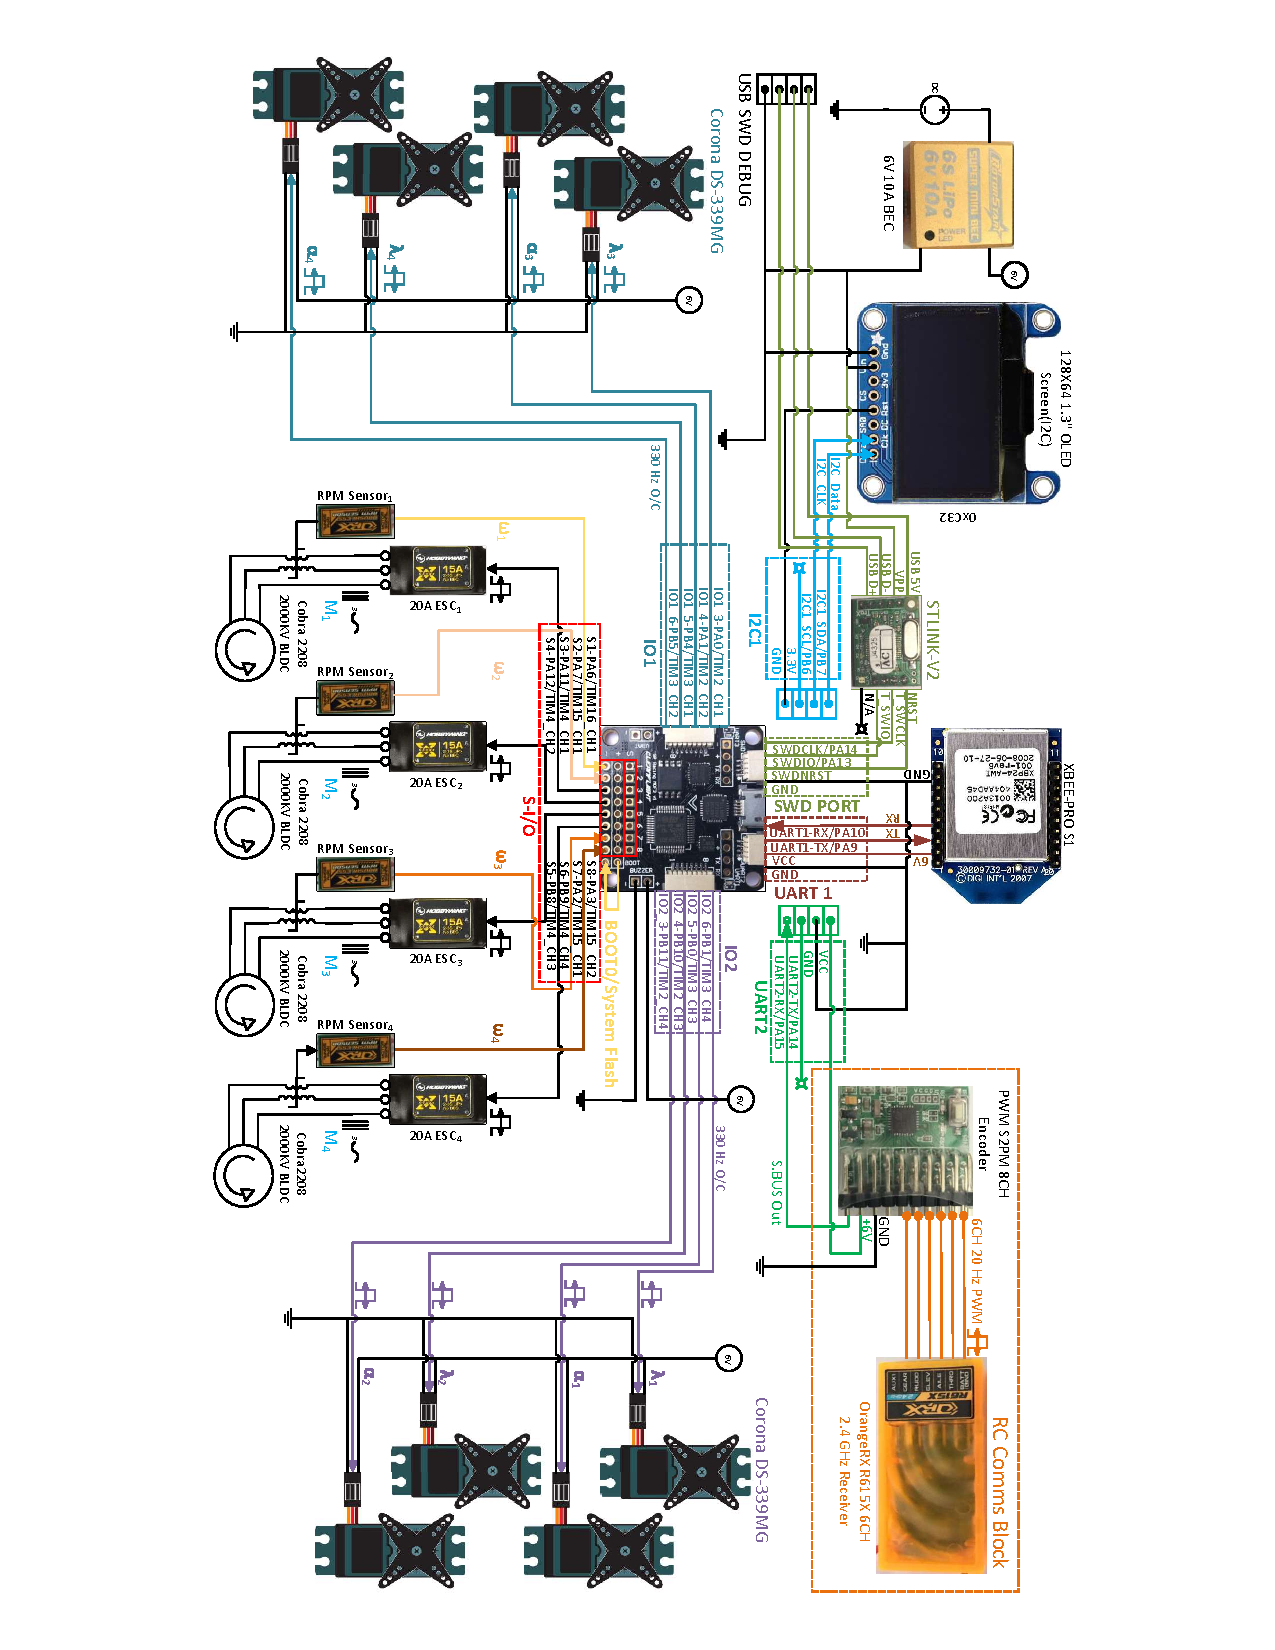
\includegraphics[clip, trim=3.5cm 1cm 3.4cm 1cm, width=0.81\textwidth]{pdfpages/electrical-schematic.pdf}
}
\end{minipage}
\vspace{-10pt}
\captionof{figure}{Hardware schematic diagram}
\label{fig:electrical-schematic}
}
%-----------------------------------------------------
\newpage
%-----------------------------------------------------
An abstracted hardware diagram for the proposed (electronic) system layout is shown in Fig:\ref{fig:electrical-schematic}. It is an illustration for the connection of different electronic peripherals to aid the on-board control system. The structure of the implemented autopilot system and control loops are addressed later. This section aims to provide a brief overview of the specific modules intended for the flight controller, their purpose and a description of how they are interfaced. No control loops or code structures are discussed yet, those are detailed in Sec:\ref{sec:control.loop} and Sec:\ref{sec:simulation.autopilot} respectively.
\par
\begin{figure}[htbp]
\begin{subfigure}{0.5\textwidth}
\centering
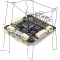
\includegraphics[width=0.95\textwidth]{figs/f3-deluxe}
\caption{SPRacing F3 deluxe flight controller}
\end{subfigure}
\begin{subfigure}{0.5\textwidth}
\centering
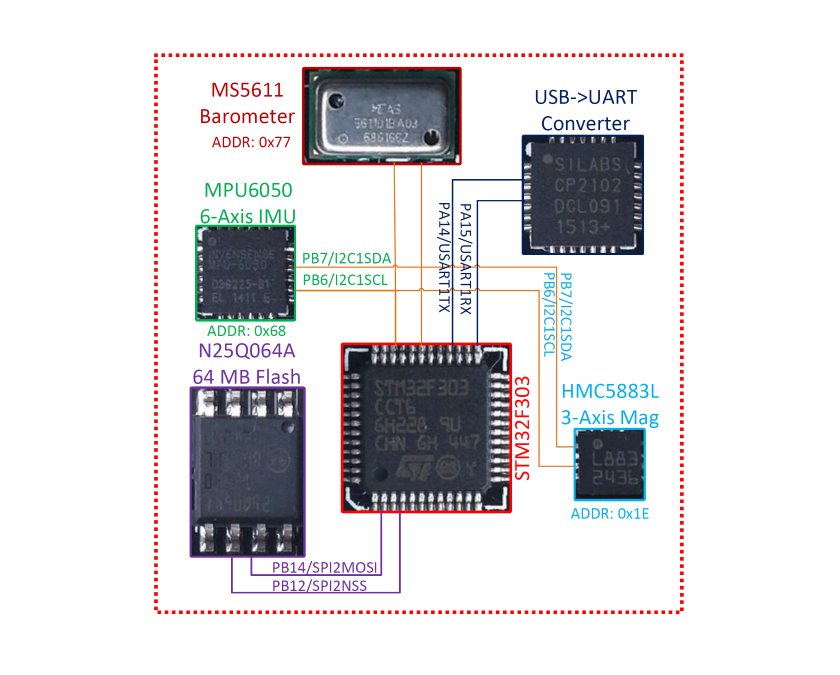
\includegraphics[width=0.95\textwidth]{figs/f3-deluxe-board}
\caption{F3 Deluxe on-board connections}
\label{fig:f3-deluxe-board}
\end{subfigure}
\caption{SPRacing F3 deluxe layout}
\label{fig:f3-deluxe-layout}
\vspace{-10pt}
\end{figure}
The embedded system is constructed around an ARM STM32F303\cite{stm32f303} based microcontroller. The micro-processor board is a commercial flight control board, specifically an SPRacing F3 Deluxe\cite{spracing}. CleanFlight or BetaFlight opensource software (from \cite{cleanflight} and \cite{betaflight} respectively) are typically used for this SPRacing F3 board; but despite open-source software its hardware specifications are  however not openly available. The reverse engineered electrical schematic for the board is included in App:\ref{app:deluxe-diagram} but a simplified overview of its internal connections is shown in Fig:\ref{fig:f3-deluxe-board}.
\par
The flight-controller has the following onboard peripherals; an I2C MPU-6050 6-axis gyroscope and accelerometer \cite{mpu6050} with an I2C connected HMC5883 magnetometer compass \cite{hmc5883}; an I2C MS5611 barometer \cite{ms5611} and finally 64 Mb of SPI flash memory. Sensor fusion for the above state estimators is dealt with subsequently in Sec:\ref{sec:simulation.state}. The caveats of Kalman filtering and discretized effects on the simulation loop are similarly discussed in that particular section.
\begin{figure}[hbtp]
\centering
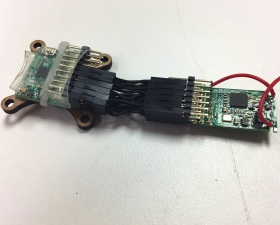
\includegraphics[width=0.55\textwidth]{figs/ppm-sbus}
\caption{SBUS converter \& 6CH receiver}
\label{fig:ppm-sbus}
\vspace{-20pt}
\end{figure}
\par
Two separate wireless communication loops are to be used. First; the system relays full state information for a complete 6-DOF X-Y-Z position and $\phi-\theta-\psi$~orientation autopilot system. Sent from an independent ground control station (\emph{GCS}) using 2.4 GHz XBEE S1 module(s)\cite{xbees1} which is connected to the flight controller via USART. Full state-estimation, using a multi-camera system (\cite{arnold}), and basic trajectory generation is performed on the GCS for the vehicle to track that trajectory. 
\par
Secondly; a partial trajectory (basic orientation) augmented pilot control input system, fail safe and secondary to the autopilot loop, is transmitted through a 6 channel 2.4 GHz radio frequency module. The secondary system allows for phsyical control without the need of a trajectory generation loop. The 6 CH received signals, otherwise permeated as six individual 20 kHz PWM signals via an OrangeRx R615x receiver \cite{r615x}, are encoded into a single proprietary S.BUS data stream (Fig:\ref{fig:ppm-sbus}). 
\par
The need for a serial bus (S.BUS) encoder, specifically using \cite{sbusencoder}, comes about as a consequence of the introduction of the 8 additional servos. As a result, there are no longer 6 free additional timer input/output channels which can be dedicated to input capture of those RC channels. Encoding the received data to a serial data line means the 6CH commands can be processed with a single RX channel by the microcontroller. The encoder implements a USART derivative communications standard called S.BUS. Shown in Fig:\ref{fig:sbus} the S.BUS data, captured with a logic analyzer \cite{saleae}, was used to ascertain the data stream's following parameters:
\par
\begin{tabularx}{\textwidth}{X X}
\begin{minipage}{\textwidth}
\begin{itemize}[itemsep=0em]
\item 25 Bytes per packet
\item 8-Bit byte length
\item 1 Start byte 0x240
\item 1 Byte of state flags
\item 1 Stop byte 0x0
\item Bytes are:
\vspace{-5pt}
\begin{itemize}[itemsep=0em]
\item MSB First
\item 1 start \& 2 stop bits
\item Even parity bit
\item Inverted
\item 100000 baud (b.s$^{-1}$)
\end{itemize}
\vspace{-5pt}
\end{itemize}
\end{minipage}
&
\begin{minipage}{\textwidth}
\begin{itemize}[itemsep=0em]
\item 22 total bytes of CH data 
\item Each channel's data is 11 bits long
\item 16CH encoded
\item Channel data is little endian prioritized
\item 14 ms idle time between packets
\item Packets are arranged:
\end{itemize}
{
$\overbrace{[0x240]}^{Start~byte}\overbrace{[8B_1][3B_2}^{CH1}|\overbrace{5B_2][6B_3}^{CH2}|\overbrace{2B_3][8B_4][1B_5}^{CH3}|\ldots$
\\
$\overbrace{7B_5][4B_6|}^{CH4}\ldots\longrightarrow\ldots\overbrace{3B_22][8B_23]}^{CH16}\overbrace{[8B_24]}^{Flags}\overbrace{[0x00]}^{Stop~byte}$
}
\end{minipage}
\\
\end{tabularx}
\begin{figure}[hbtp]
\centering
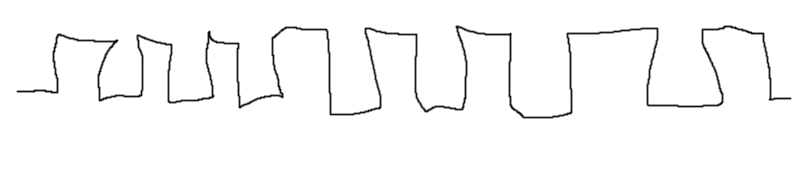
\includegraphics[width=\textwidth]{figs/sbus}
\caption{S.BUS data stream}
\label{fig:sbus}
\vspace{-10pt}
\end{figure}
\par
{\color{red}
The received information from the transmitted 6 channels is smoothed with a digital filter, using an infinite impulse response moving average filter. The filters difference equation can be as follows: 
\begin{equation}
y_n = \big(1-\frac{1}{N}\big)y_{n-1}+\frac{1}{N}x_n
\end{equation}
Moving over an average of $N=5$ samples which, each with a propagation delay of 14 ms due to S.BUS transmission, the filter has a 70 ms zero order holding time. The signal's sampling delays are sufficiently faster than the transfer times of the signals to not be consequence. 
\par
Similarly all the measured RPM signals measured by the OrangeRx RPM speed sensors are filtered over 5 samples as well. Any received signals referred to are all post filtration. Filtering for state estimation made without using the inertial-measurement unit (using the camera system) is to be performed separately on the Ground Control Station computer.}
\par
Each of the eight digital servo actuators are controlled individually from $330~[\text{Hz}]$ center aligned PWM timer output compare channels (TIM2:CH1$\rightarrow$CH4 and TIM3:CH1$\rightarrow$CH4). Output pulses typically range from $1-2~[\text{ms}]$ to linearly control the rotational position. The servo's exact range and transfer function(s) is empirically determined next in Sec:\ref{subsec:proto.design.transfer}. The four $20~[\text{A}]$ brushless DC electronic speed controllers (\emph{ESC}s) are each driven from a $20~[\text{Hz}]$ PWM output (TIM4:CH1$\rightarrow$CH4), similarly with $1-2~[\text{ms}]$ input pulse widths. 
\par
There is a total of 12 PWM output compare signals drawn from the flight controller, 8 for the servos and 4 for the ESCs. The servos are powered by a regulated $6~[\text{V}]$ DC $10~[\text{A}]$ power supply \cite{rotorstar} whilst the ESCs switch unregulated $14.1~[\text{V}]$ DC supplied from an external power tether. The DC supply could be drawn from a battery bank but that would adversely affect the weight of an already heavy platform.
\par
There is no integrated feedback for instantaneous RPM values available from the ESCs. Dedicated OrangeRX BLDC RPM sensors, \cite{orangerpm}, are used to measure each of the four motor's rotational speeds. Despite being termed \emph{brushless DC motors}, the motors are actually 3-phase motors which, when used with an ESC, behave like closed loop DC motors. The RPM sensors physically measure switching phases across two of the three motor phases, following that exact RPM can be ascertained. In general, the switching signal of a 3-Phase induction motor is shown by \cite{vfd} to be proportional to the rotational velocity:
\begin{equation}
F_{rps}=\frac{2\times F_{poles}}{\text{No. of rotor poles}}~~[\text{Hz}]
\end{equation}
The output signal generated by the OrangeRx RPM sensors varies the period of a 50\% duty cycle square wave, that wave frequency is directly proportional to the motor's pole switching frequency. The sensor output signal has a gain of 7 for the 14 pole BLDC Cobra motors. That gain is verified with the linear relationship(s) physically measured using an optical rotation sensor, plotted in Fig:\ref{fig:rpm-sensor}. Knowing exact RPM rates means the subsequent thrust and aerodynamic torques for the control plant inputs can be calculated with greater certainty.
\par
\begin{figure}[hbtp]
\begin{subfigure}{0.5\textwidth}
\centering
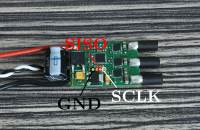
\includegraphics[width=0.98\textwidth]{figs/xrotor-20A}
\caption{XRotor 20A ESC connection guide\cite{xrotor}}
\label{fig:xrotor-20A}
\end{subfigure}
\begin{subfigure}{0.5\textwidth}
\centering
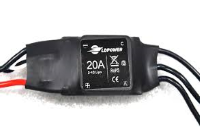
\includegraphics[width=0.98\textwidth]{figs/ldpower-20A}
\caption{LDPower 20A ESC with RPM sensor}
\label{fig:ldpower-20A}
\end{subfigure}
\caption{BLDC electronic speed controllers}
\vspace{-6pt}
\end{figure}
\par
The ESCs, although LDPower 20A devices, are re-flashed with BLHeli firmware \cite{BLHeli}. The LDPower ESCs (Fig:\ref{fig:ldpower-20A}) match Hobbywing Xrotor 20A ones (Fig:\ref{fig:xrotor-20A}) which both use SiLabs F396 microcontrollers; the same firmware can be flashed onto both MCUs. Custom BLHeli software provides greater refinement over configurations like the deflection range of inputs, but default values were used. The plot in Fig:\ref{fig:rpm-sensor-noload} shows the rotation per second, or otherwise frequency in Hz, speed curve for an unloaded motor; similarly in Fig:\ref{fig:rpm-sensor-prop} shows the speed curve when loaded for a $6\times 4.5$ prop. 
\begin{figure}[htbp]
\begin{subfigure}{0.5\textwidth}
\centering
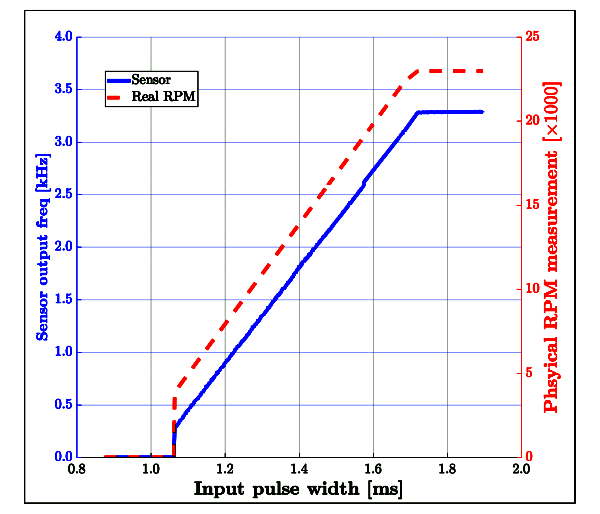
\includegraphics[width=\textwidth]{graphs/rpm-sensor-noload}
\caption{RPM sensor plot - no load}
\label{fig:rpm-sensor-noload}
\end{subfigure}
\begin{subfigure}{0.5\textwidth}
\centering
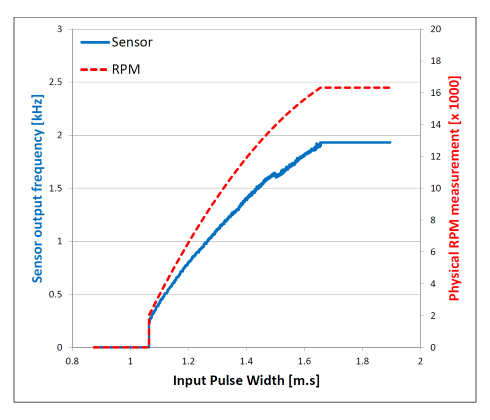
\includegraphics[width=\textwidth]{graphs/rpm-sensor-prop}
\caption{RPM sensor plot - 6X4.5 prop}
\label{fig:rpm-sensor-prop}
\end{subfigure}
\vspace{-4pt}
\caption{RPM sensor calibration plots}
\label{fig:rpm-sensor}
\vspace{-14pt}
\end{figure}
\par
The loaded speed plot for a BLDC motor with an attached prop in Fig:\ref{fig:rpm-sensor-prop} is slightly quadratic; the loaded response is due to second order aerodynamic; quadratic with respect to the propeller's revolutions per second (expanded on in Sec:\ref{subsec:dynamics.aero.bem}). Moreover, when the motor is torque loaded by the propeller, the ESC current limits rotational speeds at just over $16\times 10^3~[\text{RPM}]$.
\par
Timer channels are used to measure the varying frequency output from the RPM sensors. General purpose Timers 15 (TIM15:CH1$\rightarrow$CH2), 16 (TIM16:CH1) and 17 (TIM17:CH1) are configured to capture the input PWM signal generated by the speed sensors. Included on the I2C communciation line is an I2C O-LED display for debugging and status update purposes.
\par
Any STM32 $\mu$controller is programmed through a dedicated debugging device. The ST-Link V2\cite{st-link} is the current proprietary device which, itself, is a specially programmed STM32F10 chip. The chip connects to the dedicated \textbf{S}erial \textbf{W}ire \textbf{D}ebugging ports of the target STM (\emph{SWD-CLK, SWD-IO} \& \emph{SWD-NRST}) and is interfaced via regular USBD+ and USBD- data lines. 
%====================================================
\subsection{Actuator Transfer Functions}
\label{subsec:proto.design.transfer}
%====================================================
\subsubsection*{Servo Transfer Functions}
%====================================================
\begin{figure}[htbp]
\centering
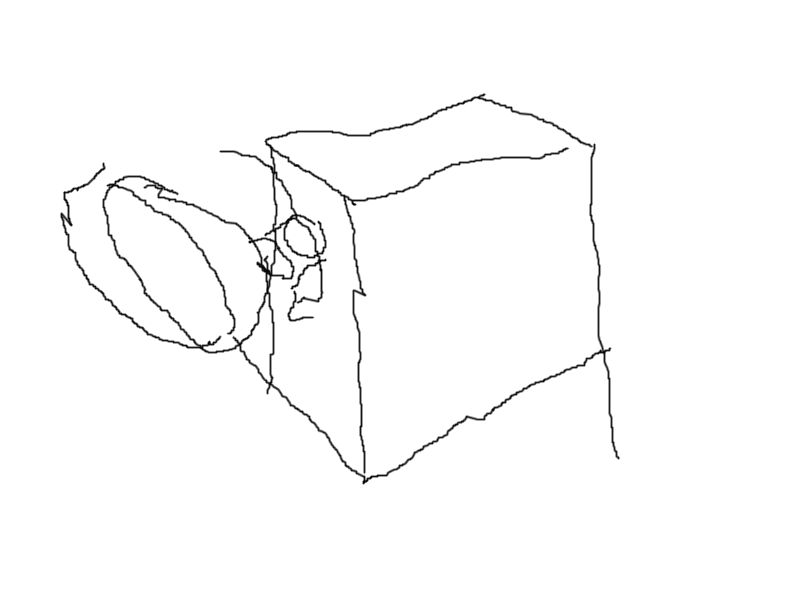
\includegraphics[width=0.6\textwidth]{figs/servo-position}
\caption{Servo transfer function test rig}
\label{fig:servo-position}
\end{figure}
The full scale deflection for digital servos are in fact greater than their quoted 180\textdegree ~range. Each servo has a rotational input range of around 230\textdegree ~(Fig:\ref{fig:servo-range}). In the prototype control loop the servos are left in open loop; the major loop controller coefficients are expected to account for minor loop actuator dynamics. With that being said, for such an expectation to be validated the simulation would need to represent the servo's response accurately. 
\par
Seeing that the 180\textdegree ~limitation was imposed as a design decision, one of the first points of contention is the effect such a constraint would have on the feasible operating trajectories. The control algorithms derived in Ch:\ref{ch:control} are first tested with an ideal, continuous rotation servo actuator with similar rate limits and transfer characteristics. Following that servo saturation limitations are introduced and the constraints to feasibly achievable trajectories are investigated in Sec:\ref{sec:simulation.autopilot}.
\begin{figure}[htbp]
\centering
\begin{subfigure}{0.49\textwidth}
\centering
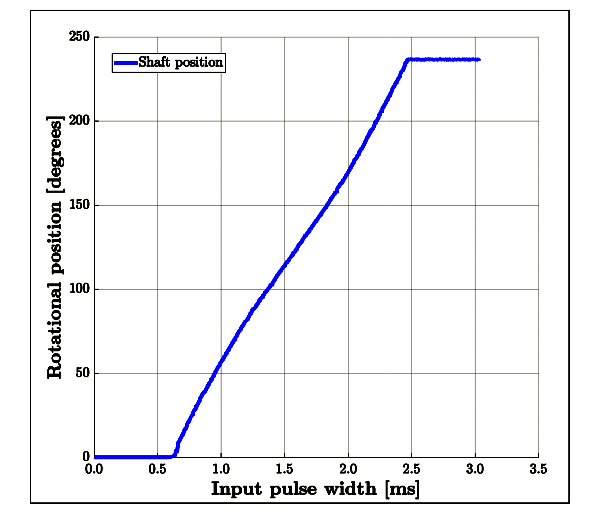
\includegraphics[width=\textwidth]{graphs/servo-range}
\caption{DS339-MG full Range}
\label{fig:servo-range}
\end{subfigure}
\begin{subfigure}{0.49\textwidth}
\centering
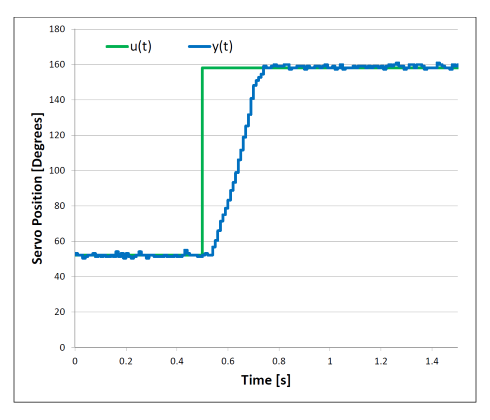
\includegraphics[width=\textwidth]{graphs/servo-step}
\caption{DS339-MG Step Response}
\label{fig:servo-step}
\end{subfigure}
\caption{Unloaded servo transfer characteristics}
\label{fig:servo-no-load}
\vspace{-10pt}
\end{figure}
\par
For the servos whose rotational range and step response are shown in Fig:\ref{fig:servo-no-load}, the relationship between the input pulse-width $x~[\text{m.s}]$ and the rotational output position $y~[\text{\textdegree}]$ is given by:
\begin{equation}\label{eq:servo-range}
y(x)=
\begin{cases}\begin{array}{ll}
0\text{\textdegree} & ~~x<0.65~\text{ms}\\
129.12x-82.64 & ~~0.64~\text{ms} \leq x \leq 2.46~\text{ms}\\
230\text{\textdegree} & ~~x>2.46~\text{ms}\\
\end{array}
\end{cases}
\end{equation}\par
In practice the equation Eq:\ref{eq:servo-range} is changed such that 0\textdegree ~offset is taken at around a 50\% input, making its operational range $\pm 90$\textdegree . Each servo is mechanically rate limited to $60\text{\textdegree}/0.15s$ or $400$ degrees per second with a dead time of $t_d\approx 1.2~[\text{ms}]$ and a (\emph{negligible}) mechanical deadband of $4~[\mu\text{s}]$. Each servo has an approximate (\emph{critically damped}) second order transfer function
\begin{subequations}\label{eq:servo-transfer}
\begin{equation}
G_{servo}(s)=e^{-t_d s}\frac{w_n^2}{s^2+2\zeta w_n s + w_n^2}
\end{equation}
\begin{equation}
=\frac{e^{-0.012s}(14.869)^2}{s^2+2(1)(14.869)s+(14.869)^2}
\end{equation}
With saturation limits from $|U(s)|$ for the PWM magnitude:
\begin{equation}
Y_{servo}(s)=
\begin{cases}\begin{array}{ll}
0\text{\textdegree} & ~~|U(s)|<0.65\\
G(s) & 0.65 \leq |U(s)| \leq 2.46\\
230\text{\textdegree} & ~~|U(s)|>2.46\\
\end{array}
\end{cases}
\end{equation}
\end{subequations}
\par
The net transfer block for the servo is shown in Fig:\ref{fig:servo-block}, including saturating nonlinearities but neglecting the afore mentioned mechanical deadband\ldots
\begin{figure}[hbtp]
\centering
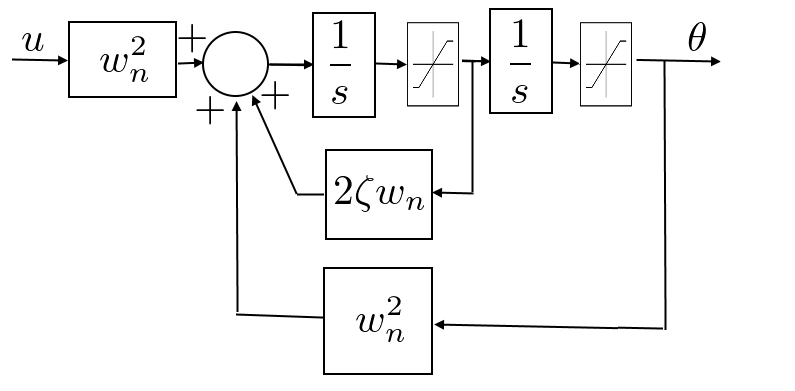
\includegraphics[width=0.8\textwidth]{figs/servo-block}
\vspace{-5pt}
\caption{Servo block diagram}
\label{fig:servo-block}
\vspace{-15pt}
\end{figure}
\par
The plot in Fig:\ref{fig:servo-step} shows the transfer characteristics, at the \emph{shaft output}, of an unloaded servo. When rotating the inertial body of the inner ring assembly, arranged as in Fig:\ref{fig:servo-inner}. Plotted in Fig:\ref{fig:servo-step-inner} is the plant response of {\color{Blue}$\mathbf{y(t)}$} which is consistent with the transfer function in Eq:\ref{eq:servo-transfer}, $\therefore G(s)_{inner}=G(s)_{servo}$. Despite rotating a load and hence requiring a greater torque. The servo's characteristics remains unchanged, even when the BLDC motor (with a $6\times4.5$ prop) with a rotational velocity of 6500 RPM is introduced, plotted {\color{Red}$\mathbf{y'(t)}$}, further increasing the torque load of the assembly as a result of the gyroscopic response, Eq:\ref{eq:prop-inertia}.
\begin{figure}[htbp]
\vspace{-6pt}
\centering
\begin{subfigure}{0.7\textwidth}
\centering
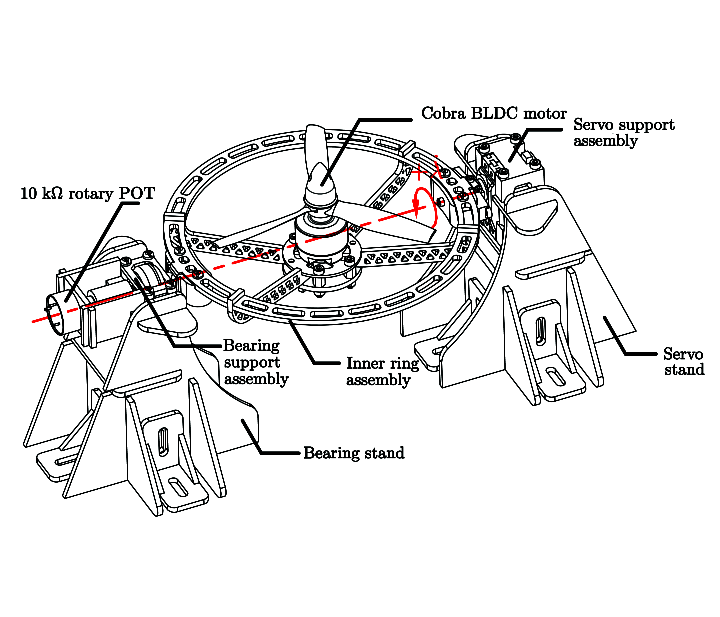
\includegraphics[width=\textwidth]{figs/servo-inner}
\vspace{-10pt}
\caption{Inner ring servo rig}
\label{fig:servo-inner}
\end{subfigure}
\\
\begin{subfigure}{0.49\textwidth}
\centering
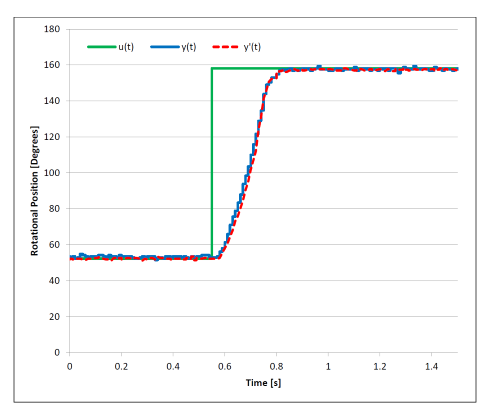
\includegraphics[width=\textwidth]{graphs/servo-step-inner}
\caption{Servo response plot}
\label{fig:servo-step-inner}
\end{subfigure}
\vspace{-4pt}
\caption{Inner ring servo characteristics}
\label{fig:servo-inner-character}
\vspace{-10pt}
\end{figure}
\par
Fig:\ref{fig:servo-step-middle} plots the step response for the servo driving the middle ring assembly. Whilst its transients remain the same oscillations are introduced at the settling point; demonstrating a second order under-damped plant. Those oscillations are as a result of the larger rotational inertia (Eq:\ref{eq:inertia.middle}), introducing flexure within the frame structure. It is important to specify that the oscillations are not at the servo's output shaft; the rotational position was measured with respect to the bearing supported shaft, coaxial to the servos (Fig:\ref{fig:servo-middle}). An under-damped transfer function needs to be used because the rotation position of the frame is to be used for force calculations in Eq:\ref{eq:motor-module-force-redirect}. Those harmonics are still present under load, plotted in {\color{Red}$\mathbf{y'(t)}$}, despite the frame being tensioned by a thrust. 
\begin{figure}[hbtp]
\vspace{-4pt}
\centering
\begin{subfigure}{0.85\textwidth}
\centering
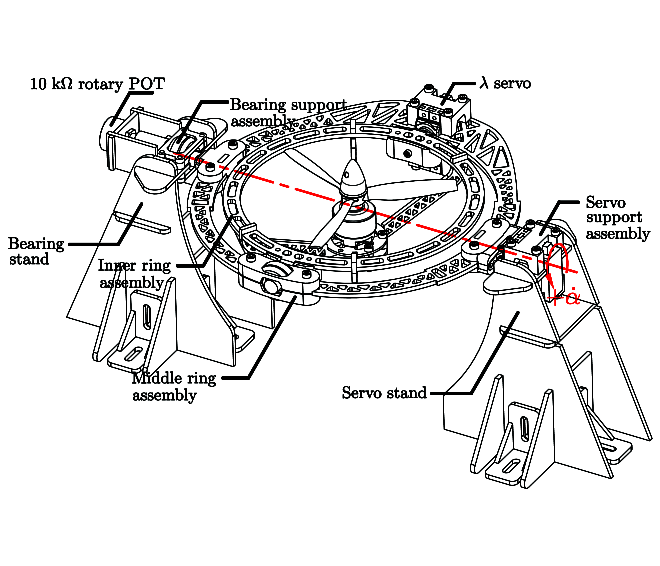
\includegraphics[width=\textwidth]{figs/servo-middle}
\vspace{-12pt}
\caption{Middle ring servo test rig}
\label{fig:servo-middle}
\end{subfigure}
\\
\begin{subfigure}{0.49\textwidth}
\centering
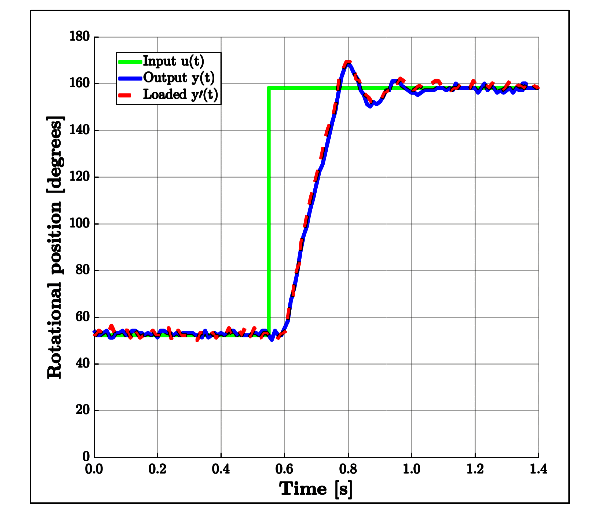
\includegraphics[width=\textwidth]{graphs/servo-step-middle}
\vspace{-6pt}
\caption{Servo response plot}
\label{fig:servo-step-middle}
\end{subfigure}
\caption{Middle ring servo characteristics}
\label{fig:servo-middle-character}
\vspace{-18pt}
\end{figure}
\par
The mechanical structure could indeed be strengthened to reduce the oscillations present in Fig:\ref{fig:servo-middle}. Strengthening the frame would introduce greater mass to an already constrained system. Instead the under-damped transfer function is included into the plant, that transfer function is:
\begin{equation}\label{eq:servo-transfer-middle}
G(s)_{middle}=\frac{e^{-0.012s}(12.591)^2}{s^2+2(0.454)(12.591)s+(12.591)^2}
\end{equation}
\subsubsection*{BLDC Transfer Functions}
Each Cobra 2208 BLDC motor, when loaded with a $6\times4.5$ propeller has a quadratic speed curve (plotted in Fig:\ref{fig:bldc-range}). This is as a result of the propeller's opposing aerodynamic drag, \emph{appromixately} proportional to the square of the propellers angular velocity (more on propeller aerodynamics in Sec:\ref{subsec:dynamics.aero.bem}).
\begin{figure}[htbp]
\centering
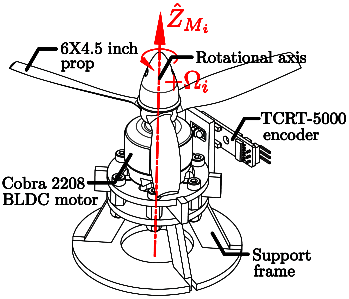
\includegraphics[width=0.44\textwidth]{figs/bldc-rpm}
\caption{BLDC rpm speed calibration and transfer function rig}
\label{fig:bldc-rpm}
\vspace{-16pt}
\end{figure}
\par
Using the BLHeli interface, the input range for the motor's speed controllers can be adjusted, but for the purposes of this project were left unchanged. That relationship between input pulse-widths to the ESC and output RPM sensor signal is given by the hybrid state equations for input range limits:
\begin{equation}
y(x)=
\begin{cases}\begin{array}{ll}
0 & ~~x<1.065~\text{ms}\\
-20593x^2 + 80187x - 60004 & ~~1.065~\text{ms} \leq x \leq 1.655~\text{ms}\\
16300 & ~~x>1.655~\text{ms}\\
\end{array}
\end{cases}
~~~\Bigg\}~~~~[\text{RPM}]
\label{eq:bldc-range}
\end{equation}
The upper limit in Eq:\ref{eq:bldc-range} and the motor's step response are both governed by the ESC's maximum current limit; in this case $20~[\text{A}]$. Imposing $10~[\text{A}]$ current limiting, a consequence of using lower power ESCs is plotted {\color{YellowGreen}$\mathbf{c(t)}$} in Fig:\ref{fig:bldc-step}, significantly restricts the motor's transient and steady-state performance. 
\begin{figure}[hbtp]
\begin{subfigure}{0.48\textwidth}
\centering
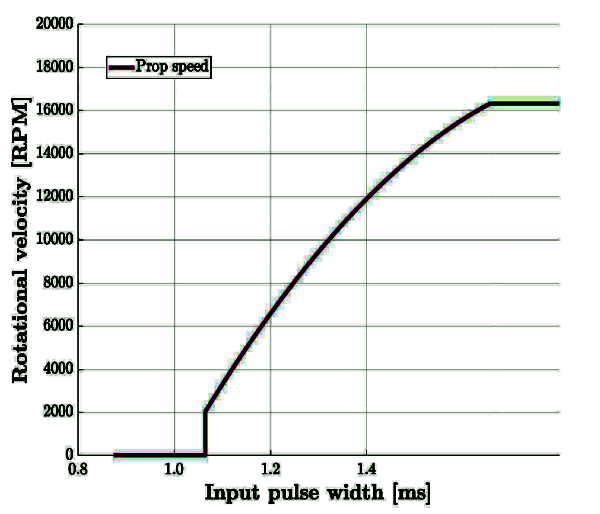
\includegraphics[width=0.98\textwidth]{graphs/bldc-range}
\caption{BLDC RPM range}
\label{fig:bldc-range}
\end{subfigure}
\begin{subfigure}{0.48\textwidth}
\centering
\includegraphics[width=0.98\textwidth]{graphs/BLDC-step}
\caption{Cobra BLDC step response}
\label{fig:bldc-step}
\end{subfigure}
\caption{BLDC motor characteristics}
\end{figure}
\par
The motor's step response, {\color{Purple}$\mathbf{y(t)}$}, has a negligible dead time and 2\textsuperscript{nd} order dynamics, with a transient time constant far faster than the servo's plant. The motor's transfer function for speed in RPM is:
\begin{subequations}\label{eq:bldc-transfer}
\begin{equation}
G_{BLDC}(s)=\frac{1}{\big(1+1.7583s\times 10^{-3}\big)\big(1+1.7494s\times 10^{-3}\big)}~~~~[\text{RPM}]
\end{equation}
And saturation limits with input $|U(s)|$ for the PWM magnitude:
\begin{equation}
Y_{BLDC}(s)=
\begin{cases}\begin{array}{ll}
0\text & ~~|U(s)|<1.065\\
G(s) & 1.065 \leq |U(s)| \leq 1.655\\
16300 & ~~|U(s)|>1.655\\
\end{array}
\end{cases}
\end{equation}
\end{subequations}
\vspace{-22pt}
%====================================================

%****************************************************
%	CHAPTER 3 - Dynamics
%****************************************************
\chapter{Kinematics \& Dynamics}
\label{ch:dynamics}
%====================================================
Generally applicable rigid body dynamics are first derived. Thereafter, those dynamics are adapted to the non-linear multibody case where constrained relative internal rotational in permitted. Following that, aerodynamic effects are investigated and incorporated into the plant's model. Finally a consolidated, quaternion based plant model is presented which is used for the later control plant development next in Chapter:\ref{ch:control}.
%====================================================
\section{Rigid Body Dynamics}
\label{sec:dynamics.rigidbody}
%====================================================
\subsection{Lagrange Derivation}
\label{subsec:dynamics.rigidbody.lagrange}
%====================================================
Fundamentally any body, rigid or otherwise, can undergo two kinds of movements, namely rotational and translation motions. Often a Lagrangian\cite{classicaldynamics,rotationrigidbody} approach for combined angular and translational movements is used to derive the differential equations of motion for each degree of freedom. The Lagrangian principle ensures that (translational and rotational) kinematic energies and potential energy are conserved throughout the system's trajectory progression. When combined with Euler-Rotational equations, the Euler-Lagrangian\cite{lagrange-formalism} formulation fully defines the aerospace 6-DOF equation set.
\par
Lagrangian formalism is regarded as especially useful in non-cartesian (\emph{spherical etc\ldots}) co-ordinate frames or multi-body systems. With that being said, a cartesian co-ordinate system was already defined in Section:\ref{subsec:proto.conventions.motoraxis}. Rigid body dynamics in a cartesian co-ordinate frame do lend themselves to Newtonian mechanics. The Newton-Euler or Euler-Lagrange formulations both stipulate the same resultant differential equations of motion. The Lagrangian operator, $\mathcal{L}$, is a term consisting of the difference between kinetic and potential energies, $T$ and $U$ respectively. Considering some generalized path co-ordinates $\mathbf{r}(t)$, for both linear $\vec{\mathcal{E}}$ and angular $\vec{\eta}$ relative positions;
\begin{equation}\label{eq:generalpath}
\mathbf{r}(t)=\begin{bmatrix}
\vec{\mathcal{E}} \\
\vec{\eta}
\end{bmatrix}
\end{equation}
The co-ordinates in Eq:\ref{eq:generalpath} are generalized here, despite being symbols commonly used to represent linear and angular positions. The generalized co-ordinates are later be refined as Cartesian body co-ordinates with respect to the inertial frame. The Lagrangian is, by definition:
\begin{subequations}
\begin{equation}\label{eq:lagrangian.a}
\mathcal{L}(\mathbf{r},\dot{\mathbf{r}},t)=T(\mathbf{r},\dot{\mathbf{r}})-U(\mathbf{r},\dot{\mathbf{r}})
\end{equation}
With kinetic and potential energy function(s) $T$ and $U$ respectively. Then introducing a rigid body's general kinetic (angular \& linear) and potential energies, in some shared reference frame. In this case the only potential energy is gravitational\footnote{Here $G=\begin{bmatrix}
0&0&-9.81
\end{bmatrix}^T~m.s^{-2}$~in the Inertial frame,$\in\mathcal{F}^I$} potential energy:
\begin{equation}\label{eq:lagrangian.b}
\mathcal{L}=
\frac{1}{2}
\begin{bmatrix}
\dot{\vec{\mathcal{E}}}^{~T}(m)\dot{\vec{\mathcal{E}}}\\
\dot{\vec{\eta}}^{~T}(\mathbb{I}_b)\dot{\vec{\eta}}
\end{bmatrix}
-
\begin{bmatrix}
m\vec{G}z\\
0
\end{bmatrix}
\end{equation}
\end{subequations}
Noting that $\mathbb{I}_b$ is the inertial tensor of the body aligned w.r.t to whichever reference frame is used. The Euler-Lagrange formulation equates partial derivatives of the Lagrangian to any generalized forces, $\mathbf{V}$, acting on the system. In this case the generalized forces or, more specifically a net force $\vec{F}_{net}$ and a net torque $\vec{\tau}_{net}$.
\begin{equation}\label{eq:euler-lagrange}
\frac{d}{dt}\bigg(\frac{\delta L}{\delta \dot{\mathbf{r}}}\bigg)-\frac{\delta L}{\delta \mathbf{r}} = \mathbf{V} = \begin{bmatrix}
\vec{F}_{net}\\
\vec{\tau}_{net}
\end{bmatrix}
\end{equation}
And taking the partial derivatives of Eq:\ref{eq:lagrangian.b} with respect to the path co-ordinates $\mathbf{r}$:
\begin{subequations}
\begin{equation}\label{eq:partial.a}
\frac{\delta L}{\delta \mathbf{r}}=\begin{bmatrix}
m\vec{G}_x\\
0
\end{bmatrix}
\end{equation}
\vspace{-5pt}
\begin{equation}\label{eq:partial.b}
\frac{d}{dt}\bigg(\frac{\delta L}{\delta \dot{\mathbf{r}}}\bigg)=\bigg[
m\frac{d}{dt}\dot{\vec{\mathcal{E}}} ~~~ \mathbb{I}\frac{d}{dt}\dot{\vec{\eta}}\bigg]^T
\end{equation}
\end{subequations}
Where $\vec{G}_x$ is the gravitation force in whichever reference frame ($\mathcal{F}^x$) the lagrangian is with respect to. In any generalized coordinate system a rotating vector's time derivative which, according to the Reynolds Transportation Theorem\cite{reynolds}, is given by:
\begin{equation}\label{eq:reynolds}
\frac{d\vec{f}}{dt_a}=\frac{d\vec{f}}{dt_b}+\vec{\omega}_{a/b}\times\vec{f}
\end{equation}
So applying that theorem (Eq:\ref{eq:reynolds}) to the partial derivatives in Eq:\ref{eq:partial.b} and further defining the generalized co-ordinates as cartesian body coordinates with respect to an inertial origin (the body frame $\mathcal{F}^b$ and inertial frame $\mathcal{F}^I$). Noting that in Eq:\ref{eq:partial.b} the place holders used for linear ($\vec{\mathcal{E}}$) and angular positions ($\vec{\eta}$) all exist in a common shared frame\footnote{In this case $\vec{\eta}\not=[\phi~\theta~\psi]^T$ seeing that the angular position $\vec{\eta}$ is defined in a common frame. $\vec{\eta}$ is \underline{NOT an Euler angle} set.}, and hence:
\begin{equation}
\frac{d}{dt}
\begin{bmatrix}
{\mathcal{E}}\\
\vec{\eta}
\end{bmatrix}
\triangleq
\begin{bmatrix}
\vec{\nu}\\
\vec{\omega}
\end{bmatrix}
\in \mathcal{F}^b
\end{equation}
It then follows that the Lagrangian Eq:\ref{eq:lagrangian.b} changes to:
\begin{subequations}
\begin{equation}
\mathcal{L}=\frac{1}{2}
\begin{bmatrix}
\vec{\nu}^{~T}(m)\vec{\nu}\\
\vec{\omega}^{~T}(\mathbb{I})\vec{\omega}
\end{bmatrix}
-
\begin{bmatrix}
m\vec{G}_b z\\
0
\end{bmatrix}
\end{equation}
\vspace{-5pt}
\begin{equation}
\frac{d}{dt}\bigg(\frac{\delta L}{\delta \dot{\mathbf{r}}}\bigg)=\bigg[
m\frac{d}{dt}\vec{\nu} ~~~ \mathbb{I}\frac{d}{dt}\vec{\omega}\bigg]^T
\end{equation}
\vspace{-5pt}
\begin{equation}
\rightarrow m\frac{d}{dt}\vec{\nu}=m\dot{\vec{\nu}}+\vec{\omega}_{I/b}\times\vec{\nu}
\end{equation}
\vspace{-5pt}
\begin{equation}
\rightarrow \mathbb{I}_b \frac{d}{dt}\vec{\omega}=\mathbb{I}_b\dot{\vec{\omega}}+\vec{\omega}_{I/b}\times\mathbb{I}_b\vec{\omega}
\end{equation}
\end{subequations}
Which, when substituted back into the Euler-Lagrange formulation Eq:\ref{eq:euler-lagrange}, results in the familiar Newton-Euler equations for linear and angular differentials, both in the body frame;
\begin{subequations}\label{eq:newton}
\begin{equation}\label{eq:newton.a}
\vec{F}_{net}=m\dot{\vec{\nu}}+\vec{\omega}_b\times m \vec{\nu} - m\mathbb{R}_I^b(-\eta) \vec{G}_I
\end{equation}
\vspace{-15pt}
\begin{equation}\label{eq:newton.b}
\vec{\tau}_{net}=\mathbb{I}_b\dot{\vec{\omega}}_b+\vec{\omega}_b\times\mathbb{I}_b\vec{\omega}_b
\end{equation}
\end{subequations}
It's important to recall that $\vec{\omega}_b\not= \dot{\vec{\eta}}$ where $\vec{\eta}=[\phi~\theta~\psi]^T$, seeing that Euler Angles are defined in sequentially rotated reference frames. So then four differential equations are often used to completely describe the entire set of state derivatives, namely:
\begin{subequations}\label{eq:states}
\begin{equation}\label{eq:states.a}
\dot{\vec{\mathcal{E}}}=\mathbb{R}_b^I(-\eta)\vec{\nu}~~~~\in\mathcal{F}^I
\end{equation}
\vspace{-10pt}
\begin{equation}\label{eq:states.b}
\vec{F}_{net}=m\dot{\vec{\nu}}+\vec{\omega}_b\times m\vec{\nu} -m \mathbb{R}_I^b(-\eta)\vec{G}_I ~~~~\in\mathcal{F}^b
\end{equation}
\newpage
\begin{equation}\label{eq:states.c}
\dot{\vec{\eta}}=\Psi(\eta)\vec{\omega}_b~~~~\in\mathcal{F}^{v2},\mathcal{F}^{v1},\mathcal{F}^I
\end{equation}
\vspace{-10pt}
\begin{equation}\label{eq:states.d}
\vec{\tau}_{net}=\mathbb{I}_b\dot{\vec{\omega}}_b+\vec{\omega}_b\times\mathbb{I}_b\vec{\omega}_b~~~~\in\mathcal{F}^b
\end{equation}
\end{subequations}
The state differentials in Eq:\ref{eq:states} can be reduced to a set of two equations. Those differentials are defined in reference frames of the state variables which they represent. The non-linear form of those equations substitutes\footnote{Originally introduced in Eq:\ref{eq:angular-rates.e}} $d\vec{\eta}/dt=\Phi(\eta)\vec{\omega}_b$ in the Lagrangian derivative, Eq:\ref{eq:partial.b}.
\begin{equation}
\frac{d}{dt}\bigg(\frac{\delta \mathcal{L}}{\delta \dot{\mathbf{r}}}\bigg)=\bigg[m\frac{d}{dt}\vec{\nu}~~~\mathbb{I}\frac{d}{dt}\dot{\vec{\eta}}\bigg]^T\Rightarrow\bigg[m\frac{d}{dt}\vec{\nu}~~~\mathbb{I}\frac{d}{dt}\Phi(\eta)\vec{\omega}_b\bigg]^T
\end{equation}
This only affects the angular component as the two kinetic energies are independent of one another. And so applying the differential chain rule:
\begin{equation}
\mathbb{I}\frac{d}{dt}\Phi(\eta)\vec{\omega}_b=\mathbb{I}\big(\Phi\dot{(\eta)}\vec{\omega}_b+\Phi(\eta)\dot{\vec{\omega}}_b \big)
\end{equation}
Drawing from \cite{autonomousrobotseuler} and recognizing that $\mathbb{I}$ must be transformed to the common intermediate Euler axes, $\mathbb{J}=\Psi(\eta)^T\mathbb{I}\Psi(\eta)$. The controllable differential equation for angular acceleration in Eq:\ref{eq:newton.b}, then in intermediate Euler frames for each angle becomes\footnote{The relationship $\dot{\Phi}=\Phi\dot{\Psi}\Phi$ was used to simplify Eq:\ref{eq:nonlinear}, the singularity in $\Phi$ still remains\ldots}:
\begin{subequations}\label{eq:nonlinear}
\begin{equation}\label{eq:nonlinear.a}
M(\eta)\ddot{\vec{\eta}}+C(\eta,\dot{\eta})\dot{\vec{\eta}}=\Psi(\eta)\vec{\tau}_{net}
\end{equation}
\vspace{-15pt}
\begin{equation}\label{eq:nonlinear.b}
M(\eta)=\Psi(\eta)^T\mathbb{I}\Psi(\eta)
\end{equation}
\vspace{-10pt}
\begin{equation}\label{eq:nonlinear.c}
C(\eta,\dot{\eta})=-\Psi(\eta)\mathbb{I}\Psi\dot{(\eta)}+\Psi(\eta)^T \big[\Psi(\eta)\dot{\vec{\eta}}\big]_{\times}\mathbb{I}\Psi(\eta)
\end{equation}
\end{subequations}
Equation \ref{eq:nonlinear.a} fully describes the state derivative $\ddot{\vec{\eta}}$ in its own frame(s). The two differential equations which describe the entire bodies motion are then:
\begin{subequations}\label{eq:rigid-frame}
\begin{equation}\label{eq:rigid-frame.a}
\vec{F}_{net}=m\dot{\vec{\mathcal{E}}}+\mathbb{R}_b^I(-\eta)\vec{\omega}_b \times m \dot{\vec{\mathcal{E}}}-m\vec{G}_I~~~~\in\mathcal{F}^I
\end{equation}
\vspace{-10pt}
\begin{equation}\label{eq:rigid-frame.b}
\vec{\tau}_{net}=\Psi(\eta)^{-1}M(\eta)\ddot{\vec{\eta}}+\Psi(\eta)^{-1}C(\eta,\dot{\eta})~~~~\in\mathcal{F}^{v2,v1,I}
\end{equation}
\end{subequations}
\par
The generalized net forces effecting the system, $\vec{F}(u)$ and $\vec{\tau} (u)$, are the system's controllable inputs and are going to be affected directly the systems actuators and their associated effectiveness function. In the general case, which is expanded upon in Section:\ref{sec:dynamics.aero}, the control inputs are typically as follows:
\begin{subequations}
The net force acting on the system is just the sum of all thrust vectors produced by rotating propellers, $T(\Omega_i)$.
\begin{equation}
\mu \vec{F} = \sum_{i=1}^4 \vec{T}(\Omega_i)
\end{equation}
Secondly the net torque is the sum of all torque arms produced from those propeller thrust vectors.
\begin{equation}
\mu \vec{\tau} = \sum_{i=1}^4 \vec{l}_i \times \vec{T}(\Omega_i)
\end{equation}
\end{subequations}
Where $\vec{T}(\Omega_i)$ is the $i^{th}$ motor's thrust vector, not necessarily in $\mathbb{R}^3$, and typically bound to the $\hat{Z}_b$ axis, $\vec{l}_i$ is that thrust vector's perpendicular displacement from the origin $\mathbf{O}_b$. The above equations are still applicable to any 6 DOF body, common simplifications applied to the system(s) for quadrotor control are explored in Appendix:\ref{app:stddynamics}. Aspects unique to (multibody) aerospace frames are now introduced. Obviously the focus is on quadrotor and tilting quadrotor platforms\ldots
%====================================================
\subsection{Rotation Matrix Singularity}\label{subsec:dynamics.rigidbody.singularity}
%====================================================
The Euler Angle singularity is often mentioned but far less common is the demonstration of exactly how that singularity \emph{mathematically} manifests itself. By definition, a singularity occurs when a loss of differentiability is encountered. In the case of an affixed 3-axis gimbal (Fig:\ref{fig:gimbal}), when an intermediary rotational angle, for example the rolling angle $\theta$, is at $\pi/2$ then the remaining two axes become co-linear (Fig:\ref{fig:gimbal-lock}). That being both pitch $\phi$ or yaw $\psi$ rotations will subsequently have the same effect. Such a situation results in what is termed as a loss of a degree of freedom.
\begin{figure}[htbp]
\begin{subfigure}{0.5\textwidth}
\centering
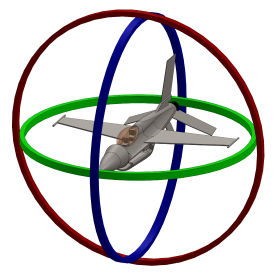
\includegraphics[width=\textwidth]{figs/gimbal}
\caption{3-Axis gimbal}
\label{fig:gimbal}
\end{subfigure}
\begin{subfigure}{0.5\textwidth}
\centering
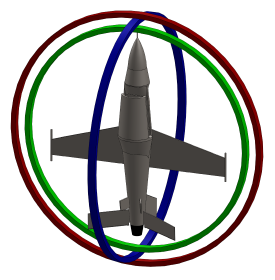
\includegraphics[width=\textwidth]{figs/gimbal-lock}
\caption{Locked gimbal with loss of DOF}
\label{fig:gimbal-lock}
\end{subfigure}
\caption{Gimbal lock}
\end{figure} 
\par
What is clear in a physical system is not necessarily as clear mathematically. An obvious loss of differentiability is manifested in the Euler Matrix $\Psi(\eta)$, Eq:\ref{eq:angular-rates.e} from Section:\ref{subsec:proto.conventions.frames}. The relation between angular velocity, in the inertial frame or inversely in the body frame, and the angular rates of the Euler Angles.
\begin{equation}\label{eq:euler-derivative}
\begin{bmatrix}
\dot{\phi}\\
\dot{\theta}\\
\dot{\psi}
\end{bmatrix}
=\begin{bmatrix}
1 & sin(\phi)tan(\theta) & cos(\phi)tan(\theta)\\
0 & cos(\phi) & -sin(\phi)\\
0 & sin(\phi)sec(\theta) & cos(\phi)sec(\theta)\\
\end{bmatrix}
\begin{bmatrix}
p\\
q\\
r
\end{bmatrix}
=\Phi(\eta)\omega_b
\end{equation}
\begin{equation}
\text{As}~\underset{{\theta \rightarrow \pi /2}}{lim}~sec(\theta),tan(\theta)\rightarrow \infty
\end{equation}
Or that $\Phi(\eta)$ is undefined at $\theta=\pi/2$. 
It's clear to see that in Eq:\ref{eq:euler-derivative} there exists an undefined singularity as $\theta\rightarrow\pi/2$. The physical consequence of this is the loss of a degree of freedom. More specifically, if one looks at how the Z-Y-X rotation (or transformation) matrices are formulated:
\begin{subequations}
\begin{equation}
\mathbb{R}_I^b = \mathbb{R}_z\mathbb{R}_y\mathbb{R}_x=\begin{bmatrix}
c_\psi & -s_\psi & 0\\
s_\psi & c_\psi & 0\\
0 & 0 & 1
\end{bmatrix}
\begin{bmatrix}
c_\theta & 0 & s_\theta\\
0 & 1 & 0\\
-s_\theta & 0 & c_\theta
\end{bmatrix}
\begin{bmatrix}
1 & 0 & 0\\
0 & c_\phi & -s_\phi\\
0 & s_\phi & c_\phi
\end{bmatrix}
\end{equation}
\begin{equation}
\mathbb{R}_I^b=\begin{bmatrix}
c_\psi c_\theta & c_\psi s_\theta s_\phi - s_\psi c_\phi & c_\psi s_\theta c_\phi + s_\psi s_\phi\\
s_\psi c_\theta & s_\psi s_\theta s_\phi + c_\psi c_\phi & s_\psi s_\theta  c_\phi - c_\psi s_\phi\\
-s_\theta & c_\theta s_\phi & c_\phi c_\theta\\
\end{bmatrix}
\end{equation}
In the case where $\theta=\pi/2$, and using trigonometric double angles;
\begin{equation}\label{eq:gimbal}
=\begin{bmatrix}
0 & c_\psi s_\phi - s_\psi c_\phi & c_\psi c_\phi + s_\psi s_\phi\\
0 & s_\psi s_\phi + c_\psi c_\phi & s_\psi c_\phi - c_\psi s_\phi\\
-1 & 0 & 0\\
\end{bmatrix}
=
\begin{bmatrix}
0 & s(\phi - \psi) & c(\phi - \psi)\\
0 & c(\phi - \psi) & s(\phi - \psi)\\
-1 & 0 & 0
\end{bmatrix}=\mathbb{R}_{x'}(\phi-\psi)
\end{equation}
\end{subequations}
Where the resultant in Eq:\ref{eq:gimbal} represents an X-axis rotation in a new intermediate frame, post a $\pi/2$ rotation in the y-axis. Through trigonometric double angles a degree of freedom is lost at $\theta=\pi/2$, when $\phi$ \& $\psi$ effect the same angle.
%====================================================
\subsection{Quaternion Dynamics}
\label{subsec:dynamics.rigidbody.quaternion}
%====================================================
An algorithm proposed in \emph{How To Avoid a Singularity When Using Euler Angles?}\cite{euleranglesingularity} suggested a solution to the problem of Euler Angle singularities. The proposed heuristic was to switch between sequencing conventions (ZYX,ZYZ etc\ldots there are 12 in total) such that the singularity is always avoided. However the implementation of such an algorithm is cumbersome and inefficient. Far more elegant is the use of \emph{quaternion} attitude representations in $\mathbb{R}^4$ (\cite{rotationsequences,quaterniondynamics,spacecraftattitutdequaternions} amongst others\ldots).
\par
A quaternion is analogous to a rotation matrix in that it represents an attitude difference between two reference frames. An $\mathbb{R}^3$ position is paramterized as a single rotation $\theta$ about a unit axis $\hat{u}$ (Sic Rodriguez Formula\cite{unwinding}). Without deliberating too much on their proof or details, a quaternion consists or a scalar component, $q_0$, and complex vector component, $\vec{q}\in \mathbb{C}^3$, such that;
\begin{equation}
Q\triangleq 
\begin{bmatrix}
q_0 \\
\vec{q}
\end{bmatrix}
~~\in\mathbb{R}^4
\end{equation}
The relationship between an Euler Angles rotation matrix $\mathbb{R}_I^b(\eta)$ and a quaternion attitude $Q_b$ is given by the Rodriguez formula:
\begin{equation}\label{eq:rodriguez}
\mathbb{R}_I^b(\eta)=\mathbb{R}(Q_b)=\mathbb{I}+2q_0[\vec{q}~]_\times+2[\vec{q}~]^2_\times
\end{equation}
Any and all quaternions, unless otherwise stated, in this dissertation are all unit quaternions\footnote{Unit quaternions are a subset of the quaternion space}, $Q\in\mathbb{Q}_u$. The need for quaternions with unity magnitude is such to ensure rotational operations don't affect the magnitude of the vector operand. A unit quaternion is defined as:
\begin{equation}
||Q||=\sqrt{{q_0}^2+\vec{q}~^2}=1
\end{equation}
Quaternion multiplication is distributive and associative, but not commutative. Specifically a quaternion multiplciation operation is equivalent to the Hamilton product. For two quaternions, $Q$ \& $P$:
\begin{subequations}
\begin{equation}
Q\otimes P = \begin{bmatrix}
q_0 \\
\vec{q}
\end{bmatrix}
\otimes
\begin{bmatrix}
p_0 \\
\vec{p}
\end{bmatrix}
\end{equation}
\vspace{-5pt}
\begin{equation}
=q_0 p_0 - \vec{q}\cdot \vec{p}+p_0 \vec{q} + q_0 \vec{p} + \vec{q}\times\vec{p}
\end{equation}
\end{subequations}
Seeing that the vector component of a quaternion is complex valued, it is natural that there exists a quaternion conjugate property. Namely:
\begin{equation}
Q^*=\begin{bmatrix}
q_0 \\
-\vec{q}
\end{bmatrix}
\end{equation}
It then follows that\footnote{Disambigation:$\mathbb{I}$ in this context is a $4\times 4$ identity matrix, not an inertial matrix}:
\begin{equation}
Q\otimes Q^* = \mathbb{I}_{4\times 4}
\end{equation}
To apply quaternion rotations to a vector $\vec{v} \in\mathbb{R}^3$ involves multiplication by two unit quaternions. 
\begin{equation}
\begin{bmatrix}
0 \\
\vec{v}~'
\end{bmatrix}
=Q\otimes
\begin{bmatrix}
0 \\
\vec{v}
\end{bmatrix}
\otimes Q^*
\end{equation}
Mostly, the zero scalar components are omitted in a rotation (\emph{or transformation}) operation, such that it is recognized the vector operands are substituted with quaternions.
\begin{equation}\label{eq:quaternion-rotation}
\vec{v}~'=Q \otimes (\vec{v}) \otimes Q^*
\end{equation} 
In the case of rigid body attitude representation, $Q_b$ is the quaternion which represents the difference between $\mathcal{F}^b$ and $\mathcal{F}^I$. A quaternion operator is equivalent to a rotation matrix operation:
\begin{equation}
\mathbb{R}_I^b \underset{Q}{\iff} Q_b \otimes (.) \otimes Q_b^*
\end{equation}
A quaternion time derivative, with $Q_\omega$ being a quaternion with a vector component equal to angular velocity $\omega\in\mathcal{F}^b$ and a zero scalar component, is given by:
\begin{equation}
\frac{d}{dt}Q_b=\frac{1}{2}Q_b\otimes Q_{\omega}=\begin{bmatrix}
-\frac{1}{2}\vec{q}^{~T} \vec{\omega}_b\\
\frac{1}{2}\big([\vec{q}~]_\times+q_0\mathbb{I}\big)\vec{\omega}_b
\end{bmatrix}
\end{equation}
Using quaternions to represent attitudes negates the need for an Euler Matrix, $\Phi(\eta)$, to represent attitudes and their rates. A body quaternion is fully defined in the body frame. The first quaternion time derivative replaces Eq:\ref{eq:states.a}\& Eq:\ref{eq:states.c};
\begin{subequations}
\begin{equation}
\dot{\mathcal{E}}=\mathbb{R}_b^I(-\eta)\vec{\nu}\underset{Q}{\iff}Q_b\otimes\vec{\nu}\otimes Q_b^*
\end{equation}
\vspace{-10pt}
\begin{equation}
\dot{\eta}=\Phi(\eta)\vec{\omega}_b\underset{Q}{\iff}\dot{Q}=\frac{1}{2}Q_b\otimes Q_\omega
\end{equation}
\end{subequations}
Second order derivatives for quaternion acceleration aren't as useful as their velocity counterparts. The second order derivative is mentioned here however it's only relevant to quaternion backstepping in the control chapter. If possible, quaternion accelerations are mostly avoided due to their complexity;
\begin{equation}
\ddot{Q}\big(\dot{Q},Q,t)=\dot{Q}\otimes Q^* \otimes \dot{Q}+\frac{1}{2}Q\otimes \big[\mathbb{I}_b^-1(\tau-4(Q^*\otimes \dot{Q})\times(\mathbb{I}_b(Q^*\otimes \dot{Q}))\big]
\end{equation}
%====================================================
\subsection{Quaternion Unwinding}
\label{subsec:dynamics.rigidbody.unwinding}
%====================================================
Although quaternions are better than Euler angles and lack the associated singularity, they do contain one caveat. Seeing that a quaternion $Q=[q_0~\vec{q}~]^T$ represents an attitude orientation of a body in $\mathbb{R}^3$ using $\mathbb{R}^4$ variables there exists what is called dual coverage\cite{unwinding}.
Each unit quaternion, stemming from Euler-Rodriguez theorem, is parametrized such that the quaternion operation represents an eigenaxis rotation of $\theta$ about an axis $\hat{u}$ such that:
\begin{equation}
Q=\begin{bmatrix}
q_0\\
\vec{q}
\end{bmatrix}=
\begin{bmatrix}
cos(\theta/2)\\
sin(\theta/2)\hat{u}
\end{bmatrix}
\end{equation}
That rotation is executed through the quaternion operator Eq:\ref{eq:quaternion-rotation}. As a result its clear to see that for each unique attitude in 3-Dimensions there exist two quaternions which correlate to the same position. Namely:
\begin{subequations}
\begin{equation}
Q =
\begin{bmatrix}
q_0 \\
\vec{q}
\end{bmatrix}
=
\begin{bmatrix}
cos(\theta/2)\\
sin(\theta/2)\hat{u}
\end{bmatrix}
.
\end{equation}
And seeing that $\theta=2\pi-\theta$, then;
\begin{equation}
Q=\begin{bmatrix}
cos(\pi - \theta/2)\\
sin(\pi - \theta/2)\hat{u}
\end{bmatrix}
=
\begin{bmatrix}
-cos(\theta/2)\\
sin(\theta/2)\hat{u}
\end{bmatrix}
\end{equation}
\end{subequations}
Every physical attitude in $\mathbb{R}^3$ has two corresponding quaternions in $\mathbb{R}^4$; $[\pm q_0~\vec{q}~]^T$. A consequence of this is two possible error state trajectories for every attitude difference. A clockwise $\theta$ rotation and an anticlockwise $2\pi-\theta$ negative rotation. This could lead to an erroneous and unnecessary "unwinding" of a complete counter revolution as a result of a dual covered error state. 
\par
Often the sign scalar component of the attitude quaternion error (Section:\ref{subsec:control.attitude.quaternion}) is simply neglected or assumed positive. As such for attitude controllers the requirement is that for positive and negative scalars the control input is consistent:
\begin{equation}
\nu_d=h([q_0~\vec{q}~]^T,t)=h([-q_0~\vec{q}~]^T,t)
\end{equation}
Or more simply that $Q_e=[|q_0|~\vec{q}~]^T$. The most simple solution which adheres to that constraint is to simply neglect the scalar component and use $h(\vec{q}_e,t)$. A positive quaternion scalar will always ensure that an error state represents a right-handed clockwise rotation. If the resolution of trajectory co-ordinates generated is sufficiently high enough, the control plant will never encounter a problem.
\par
One proposal in \emph{Nonlinear Quadcopter Attitude Control}\cite{nonlinearquadcopter} suggested using a \emph{signum} operator to design the signs of the controller coefficients for the virtual control plant input. 
\begin{subequations}\label{eq:signum-unwinging}
\begin{equation}
\vec{\omega}_d=\frac{2}{\tau}sgn(q_0)\vec{q}
\end{equation}
\vspace{-10pt}
\begin{equation}
sgn(\vec{q})=
\begin{cases}\begin{array}{ll}
1 & ~~\vec{q}\geq 0\\
-1 & ~~\vec{q}< 0\\
\end{array}
\end{cases}
\end{equation}
\end{subequations}
The resultant \emph{hybrid} controller provides global asymptotic stability, but only in the case that the eigenaxis angle $\theta\leq \pm\pi$. The control law described in Eq:\ref{eq:signum-unwinging} would still need the control torques to be designed from the angular velocity virtual control input.
\par
An alternative proposal \cite{unwinding} was to lift the quaternion error-state back into $\mathbb{R}^3$ using the Rodriguez formula, Eq:\ref{eq:rodriguez}. The mapping back to $\mathbb{R}^3$ effectively ensures that $\theta$ is minimized, or that the error-state imposes the shortest possible rotation between the reference and desired body frames.
%====================================================
\section{Multibody Nonlinearities}
\label{sec:dynamics.nonlinearities}
%====================================================
Typically multibody dynamics are solved (and simulated) as a series of interactions and responses. There are different schools of thought which have proposed various methodologies for stepping through the systems dynamics [Sic Implicit Euler\cite{physicallybased,multibodydynamics}]. For the prototype design here, only relative rotational motion is permissible between the interconnected rigid bodies. Each body is considered independently, as free and rigid, whose constraint torques induced from excitation are imposed on sequential rotational joints. Opposed to those torques are Newtonian responses of importance which manifest as what is termed \emph{gyroscopic} and \emph{inertial} torques. 
\par
A distinction must be made between torque responses here and those of Eq:\ref{eq:states.d}. The latter being a response to be compensated for and the formed being something which can be exploited by the control allocation algorithm in Section:\ref{sec:control.allocation}. The multibody analysis which follows is a very Newtonian approach in that each body involved is resolved independently and relative responses are transferred onto the inducing body.
%====================================================
\subsection{Relative Rotational Gyroscopic \& Inertial Torques}
\label{subsec:dynamics.nonlinearities.gyrotorques}
%====================================================
The torque response induced from relative rotations, the only permissible relative motion, between each connected rigid body are transferred from interacting bodies as a result of Newtons second law of rotational motion. For each of the motor modules' pitching or rolling motion, the servo motors apply some torque for that rotation. Opposed to the rotational motion are both inertial and gyroscopic response(s) of that body being acted upon. The latter being a consequence of a vector's time derivative in a rotating frame, Eq:\ref{eq:reynolds}.
\par
Each of the four motor modules are symmetrical and as such the induced torque response characteristics for one module can be extrapolated through a reference frame rotation. Seeing that each relative rotation from the actuator set $u\in\mathbb{U}$ is actuated independently and upon a different body, their responses are calculated separately too.
\par
Drawing again from Lagrangian theory\footnote{The generalized linear kinetic energy for each module is an extension of that in Eq:\ref{eq:rigid-frame.a} and is independent of any of the actuator positions.} and considering only the rotational kinetic energy for the inner ring assembly $\mathcal{F}^{M_i}$, there are no permissible transnational motions between each body and as such there is no linear kinetic energy contribution. The Lagrangian for the inner ring is formed, with concern on the effect $\lambda_i$ has on the system:
\begin{equation}
\mathcal{L}_{M_i}=\frac{1}{2}\vec{\Omega}_i^{~T}\big(\mathbb{I}_{p}\big)\vec{\Omega}_i+\frac{1}{2}\dot{\vec{\lambda}}_i^{~T}\big(\mathbb{I}_{\lambda}\big)\dot{\vec{\lambda}}_i
\end{equation}
Where $\mathbb{I}_p$ is the propeller's rotational inertia about its $\hat{Z}$ axis and $\mathbb{I}_\lambda$ being the inner ring's inertia defined in Eq:\ref{eq:inertia.inner.a}. Noting that $\vec{\Omega}_i=[0~~0~~\Omega_i]^T\in\mathcal{F}^{M_i}$ and $\dot{\vec{\lambda}}_i=[\dot{\lambda}_i~~0~~0]^T\in\mathcal{F}^{M_i'}$, the two contributors are not in a common frame. As such the equation \footnote{$\dot{\vec{\lambda}}_i'$ is superfluous but included for completeness} changes to:
\begin{subequations}
\begin{equation}
\mathcal{L}_{M_i}=\frac{1}{2}\vec{\Omega}_i^{~T}\big(\mathbb{I}_{p}\big)\vec{\Omega}_i+\frac{1}{2}\dot{\vec{\lambda}}_i'^{~T}\big(\mathbb{I}_{\lambda}\big)\dot{\vec{\lambda}}_i'
\end{equation}
\vspace{-10pt}
\begin{equation}
\dot{\vec{\lambda}}_i'=Q_x^*(-\lambda_i)\otimes\big(\dot{\vec{\lambda}}_i\big)\otimes Q_x(-\lambda_i)\Rightarrow \dot{\vec{\lambda}}_i'=\dot{\vec{\lambda}}_i
\end{equation}
\end{subequations}
Where both $\mathbb{I}_{p}$ and $\mathbb{I}_{\lambda}$ are taken W.R.T to their rotational centre(s). Recalling the Euler-Lagrange formulation from Eq:\ref{eq:euler-lagrange} with generalized co-ordinates\footnote{Relative to the body frame and not the inertial frame because Eq:\ref{eq:states.d} accounts for the inertial response of the entire body frame. Here the induced relative responses are of concern} $\mathbf{u}(t)$ of $\mathcal{F}^{M_i}$ relative to $\mathcal{F}^b$.
\begin{equation}
\frac{d}{dt}\bigg(\frac{\delta L}{\delta \dot{\mathbf{u}}}\bigg)-\frac{\delta L}{\delta \mathbf{u}} = \mathbf{V} = \vec{\tau}_{net}
\end{equation}
Then:
\begin{subequations}
\begin{equation}
\frac{d}{dt_b}\bigg(\frac{\delta\mathcal{L}}{\delta\dot{\mathbf{u}}}\bigg)=\frac{d}{dt_{M_i}}\mathbb{I}_p\vec{\Omega}_i+\vec{\omega}_{M_i/b}\times\mathbb{I}_p\vec{\Omega}_i+\frac{d}{dt_{M_i}}\mathbb{I}_{\lambda}\dot{\vec{\lambda}}_i+\vec{\omega}_{M_i/b}\times\mathbb{I}_{\lambda}\dot{\vec{\lambda}}_i
\end{equation}
With $\vec{\omega}_{M_i/b}$ being the net angular velocity of the inner ring frame relative to the body frame:
\begin{equation}
\vec{\omega}_{M_i/b}= Q_x^*(-\lambda_i)Q_y^*(-\alpha_i)\otimes\dot{\vec{\alpha}}_i\otimes Q_y(-\alpha_i)Q_x(-\lambda_i)+Q_x^*(-\lambda_i)\otimes\dot{\vec{\lambda}}_i\otimes Q_x(-\lambda_i)
\end{equation}
The net torque from a $\lambda_i$ rotation, induced in the motor module frame $\mathcal{F}^{M_i}$, can be grouped into second order \emph{Inertial} and first order \emph{Gyroscopic} components. Depending on the fidelity of the model or aggressiveness of control actions taken, higher order induced terms could be ignored.
\begin{equation}\label{eq:torque-induced-inner}
\vec{\tau}_\lambda=\underbrace{\mathbb{I}_p\dot{\vec{\Omega}}_i+\mathbb{I}_{\lambda}\ddot{\vec{\lambda}}_i}_{Inertial}+\underbrace{\vec{\omega}_{M_i/b}\times\mathbb{I}_p\vec{\Omega}_i+\vec{\omega}_{M_i/b}\times\mathbb{I}_{\lambda}\dot{\vec{\lambda}}_i}_{Gyroscopic}~~~~\in\mathcal{F}^{M_i}
\end{equation}
\end{subequations}
Similarly for the middle ring , with inertia a function of the $\lambda$ angle $\mathbb{I}_{\alpha}(\lambda_i)$ from Eq:\ref{eq:inertia.middle.c}, with generalized co-ordinates $\mathbf{v}(t)$ of $\mathcal{F}^{M_i'}$ relative to $\mathcal{F}^b$:
\begin{subequations}
\begin{equation}
\mathcal{L}_{M_i'}=\frac{1}{2}\dot{\vec{\alpha}}_i^{~T}\big(\mathbb{I}_{\alpha}(\lambda_i)\big)\dot{\vec{\alpha}}_i
\end{equation}
\vspace{-10pt}
\begin{equation}
\frac{d}{dt_b}\bigg(\frac{\delta L}{\delta \dot{\mathbf{v}}}\bigg) = \frac{d}{dt_{M_i'}}\mathbb{I}_\alpha(\lambda_i)\dot{\vec{\alpha}}_i+\vec{\omega}_{M_i'/b}\times\mathbb{I}_\alpha(\lambda_i)\dot{\vec{\alpha}}_i
\end{equation}
\vspace{-5pt}
\begin{equation}
\vec{\omega}_{M_i'/b}=Q_y^*(-\alpha_i)\otimes\dot{\vec{\alpha}}_i\otimes Q_y(\alpha_i)
\end{equation}
Which are also grouped into first and second order components.
\begin{equation}
\vec{\tau}_\alpha(\lambda_i)=\underbrace{\mathbb{I}_{\alpha}(\lambda_i)\ddot{\vec{\alpha}}_i}_{Inertial}+\underbrace{\vec{\omega}_{M_i'/I}\times\mathbb{I}_{\alpha}(\lambda_i)\dot{\vec{\alpha}}_i}_{Gyroscopic}~~~~\in\mathcal{F}^{M_i'}
\end{equation}
\end{subequations}
Each of the induced torques, $\vec{\tau}_\lambda$ and $\vec{\tau}_\alpha(\lambda_i)$, occur in intermediary frames associated with the inner and middle ring assemblies. As such, their negative responses effect\footnote{Depending on dynamic equations used it could  effect Eq:\ref{eq:rigid-frame.b}. However the equations Eq:\ref{eq:rigid-frame} are inconsequential when using quaternion dynamics.} Eq:\ref{eq:states.d}, and need to be transformed to the body frame.
\begin{equation}
\tau(u)=\sum_{i=1}^4 -Q_{M_i}\otimes \tau_{\lambda_i}(u)\otimes Q_{M_i}^*-Q_{M_i'}\otimes \tau_{\alpha_i}(u) \otimes Q_{M_i'}^*~~~\in\mathcal{F}^b
\end{equation}
The above responses are pertinent to simulation and plant dependent compensation. The simulation environment is structured such that the torques are produced as responses from Newtonian movement at every step interval. In due course it would be more efficient (and less stiff) to exploit an implicit Euler\cite{physicallybased,multibodydynamics} coordinate system in substitution for the cartesian response equations developed above. However this was not implemented in Chapter:\ref{ch:simulation}.
%====================================================
\section{Aerodynamics}
\label{sec:dynamics.aero}
%====================================================
The relationship between a propeller's rotational speed, $\Omega_i$, and its produced thrust, $\vec{T}(\Omega_i)$, is more complicated than the quadratic simplification taken at static conditions which most papers puport. The thrust is mostly dependent on the incident air velocity entering the propellers rotational plane, namely the component of the body velocity normal to the propeller's plane. Parallel fluid velocity to the propeller contributes to aerodynamic drag. The combination of aerodynamic Blade-element\cite{bem,forwarddescent} and fluid-dynamics Momentum (\emph{disc actuator}) theories produces an integral term taken across the propellers length which accurately models the aerodynamic thrust and torque functions. A verbose presentation of all aerodynamic effects experienced by a quadrotor's propeller(s) is thoroughly detailed in \cite{bladesforquadrotors}.
%====================================================
\subsection{Propeller Torque and Thrust}
\label{subsec:dynamics.aero.bem}
%====================================================
\emph{\color{Gray} A feasible situation which the prototype could encounter is where an upstream propeller provides to the incident fluid flow to another downstream propeller. Such a situation presents a complex fluid dynamics \& wake effects problem\footnote{Propeller overlapping effects are investigated in \cite{configurationpropulsion}} but remains open to further research. To expedite the system I.D process some simplifications are applied to the aerodynamics to construct an approximate model.}
\par
The rotation of a propeller applies a thrust force, $\vec{T}$, on the fluid stream\footnote{Only perpendicular mass flow across the propeller's plane is considered.} in which it acts. That fluid stream (Fig:\ref{fig:bem-flow}) has an incident head velocity, $v_\infty$, and slip stream velocity from the rotational plane, $v_s$. There is then some relationship about the change of fluid flow applied by the propeller's rotation. That relationship is then given by:
\begin{equation}
v_ s = \Delta v + v_\infty
\end{equation}
Where $\Delta v$ is the change in velocity added to the fluid by the propeller blade's profile. The propeller induces a velocity directly in front of it's rotational plane, $v_i$, such that the net fluid flow into the plane is $v_b=v_i+v_\infty$. Bernoulli's principle$^{\dagger}$ has it that net fluid flow through that plane is
\begin{equation}\label{eq:bernoulli}
v_b = \frac{1}{2} ( v_s - v_{\infty} ) = \frac{1}{2} \Delta v = \frac{1}{2} v_s \big|_{v_\infty=0}
\end{equation}
\begin{figure}[htbp]
\centering
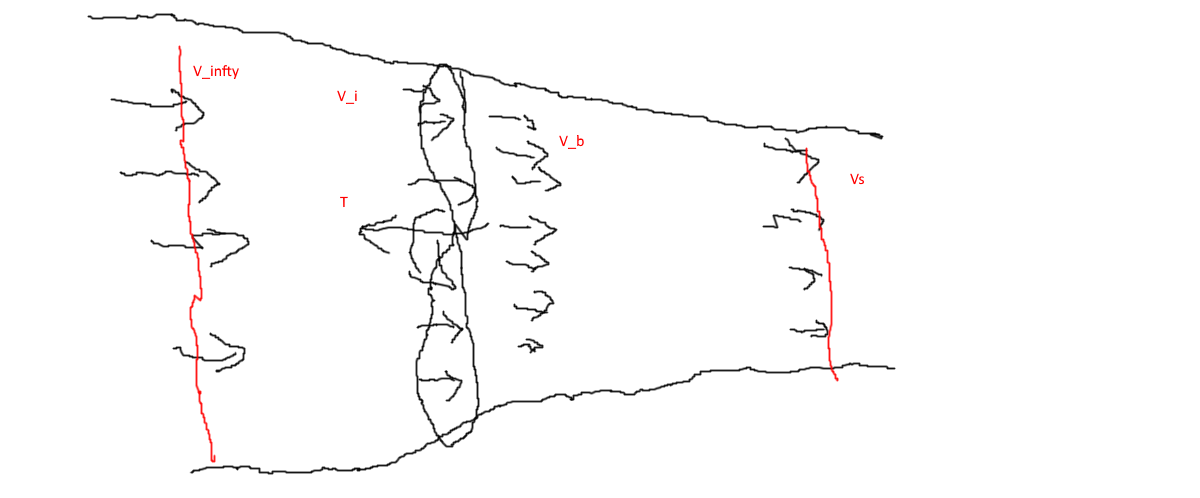
\includegraphics[width=0.7\textwidth]{figs/bem-flow}
\caption{Disc Actuator Propeller Planar Flow}
\label{fig:bem-flow}
\end{figure}
\par
And as such, stemming from classical Disc Actuator$^{\dagger}$ (\emph{momentum}) theory, the thrust acting on the fluid is a function of mass flow rate and change in velocity (pressure differential).
\begin{equation}\label{eq:prop-mass}
\vec{T}=(A_b v_b)\Delta v = \rho \pi R_b^2v_b \Delta v = \rho \pi R_b^2(v_i+v_\infty)\Delta v = \frac{1}{2} \rho \pi R_b^2 \Delta v^2
\end{equation}
Indeed Eq:\ref{eq:prop-mass} can be solved as a function of aerodynamic propulsive power expended, $P=\vec{T}v$. However that relationship between rotational kinetic power transferred is tenuous at best due to many compounded parasitic losses. In practice, the local fluid velocity over the propeller isn't purely normal to its plane. There are axial and tangential induced velocity components. Following this, induction factors can be defined which are:
\begin{subequations}\label{eq:induction-factors}
\begin{equation}\label{eq:induction-axial}
v_i=a v_\infty
\end{equation}
\vspace{-15pt}
\begin{equation}\label{eq:induction-tangential}
v_\theta=a' \Omega R
\end{equation}
\end{subequations}
From Eq:\ref{eq:induction-factors} the velocity components can be written as functions of free stream velocity $v_\infty$.
\begin{subequations}
\begin{equation}
v_b=(1+a)v_\infty
\end{equation}
\vspace{-15pt}
\begin{equation}
v_s=(1+2a)v_\infty
\end{equation}
\end{subequations}
And from the tangential fluid flow there is then an angular moment rate across the propeller plane too. This produces a torque response to the rotational motion about the propeller's axis of rotation, analogous to Eq:\ref{eq:prop-mass}.
\begin{equation}
\vec{Q}=\rho\pi R_b^3 (v_\theta-v_\infty) v_b 
\end{equation}
Blade-element theory analyses incremental aerofoil sections $dr$ of a propeller profile (Fig:\ref{fig:bem-profile}) at some radius $r$. Net local velocity across a single elemental aerofoil profile $\vec{U}$ is calculated as:
\begin{equation}
\vec{U}=\sqrt{(v_\infty+v_i)^2+(v_\Omega+v_\theta)^2}
\end{equation}
\begin{figure}[htbp]
\centering
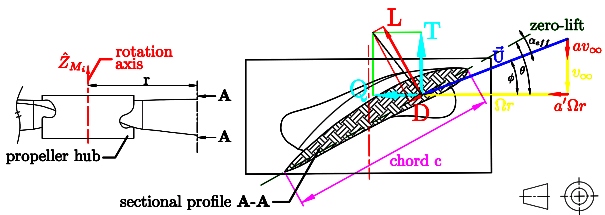
\includegraphics[width=0.9\textwidth]{figs/bem-profile}
\caption{Blade element profile at radius r}
\label{fig:bem-profile}
\end{figure}
Each elemental profile, of chord length $c$, has a local pitch, $\theta$, of its aerofoil profile relative to the horizontal. Local fluid velocities make their own an angle of attack $\phi$ at which the local propeller section encounters the fluid flow:
\begin{equation}
\phi=\theta-\alpha_{effective}
\end{equation}
That local angle of attack changes with the inflow magnitude $v_\infty$ and the induced axial velocity $v_i$. That ratio is given as:
\begin{equation}
\phi=tan^{-1}\bigg(\frac{v_\infty+v_i}{v_\Omega+v_\theta}\bigg)=tan^{-1}\bigg(\frac{v_\infty(1+a)}{\Omega r(1+a')}\bigg)
\end{equation}
\par
The in-plane fluid flow $\vec{U}(r,\phi)$, for an element at radius $r$ with a local angle of attack $\phi$, then contributes towards elemental lift and drag forces as a function of dimensionless lift, $C_L$, and drag, $C_D$, coefficients\footnote{The lift and drag coefficients are determined by the aerofoil's characteristics, but would be constant across the length of a variable pitch hinged propeller\ldots}.
\begin{subequations}
\begin{equation}
\Delta L=\frac{1}{2}\rho \vec{U}(r,\phi)^2 c C_L
\end{equation}
\vspace{-10pt}
\begin{equation}
\Delta D=\frac{1}{2}\rho \vec{U}(r,\phi)^2 c C_D
\end{equation}
\end{subequations}
With air density $\rho$ and local chord length $c$. Those lift and drag forces as components parallel and perpendicular to the plane of rotation are thrust $T$ and torque $F_x$ forces (Fig:\ref{fig:bem-profile}).
\begin{subequations}
\begin{equation}\label{eq:element-thrust}
dT=\frac{1}{2}\rho\vec{U}(r,\phi)^2c\big(C_L cos(\phi)+C_D sin(\phi)\big).dr
\end{equation}
\vspace{-10pt}
\begin{equation}\label{eq:element-drag}
dF_x=\frac{1}{2}\rho\vec{U}(r,\phi)^2c\big(C_L sin(\phi)+C_D cos(\phi)\big).dr
\end{equation}
\vspace{-10pt}
\begin{equation}\label{eq:element-torque}
\rightarrow dQ = \frac{1}{2}\rho\vec{U}(r,\phi)^2c\big(C_L sin(\phi)+C_D cos(\phi)\big)r.dr
\end{equation}
\vspace{-10pt}
\begin{equation}\label{eq:element-power}
\rightarrow dP = \Omega r dF_x .dr
\end{equation}
\end{subequations}
Typically a power term, Eq:\ref{eq:element-power}, is given in lieu of torque or drag terms, Eq:\ref{eq:element-torque} or Eq:\ref{eq:element-drag}. Then calculating forces and torques as per momentum theory for each element, in terms of tangential and axial induction factors:
\begin{subequations}
\begin{equation}
dT=\rho 4 \pi r^2 v_\infty(1+a)a.dr
\end{equation}
\vspace{-10pt}
\begin{equation}
dP=\rho 4 \pi r^2 v_\infty(1+a)\Omega r (1+a').dr
\end{equation}
\end{subequations}
Then equating momentum and element terms together produces the blade-element momentum equation(s) for thrust and power produced by a propeller. Following a few assumptions, most importantly that the lift coefficient $C_L$ is a linear function of the effective angle of attack $\alpha_{eff}$.
\par
The lift curve gradient ,$a_L$, for an ideally twisted blade, like the fixed pitch propellers under consideration here, is typically $2\pi$ such that $C_L=2\pi(\theta-\phi)$. And assuming that tangential induced velocities $v_\theta$ are small (or that the tangential induction factor $a'<<1$) when compared to the propeller's speed $\Omega r$. Similarly the net inflow and axial induced velocities $v_\infty + v_i<<\Omega r$.\footnote{Small angle approximations then apply to $cos(\phi+\alpha_{eff})\approx 1$ and $sin(\phi+\alpha_{eff})\approx \phi+\alpha_{eff}$}
\begin{subequations}
\begin{equation}\label{eq:bem-thrust}
T=\int_{r=0}^R \frac{1}{2} a_L b c \rho (\Omega r)^2 \big(\theta-\frac{v_\infty+v_i}{\Omega r}\big).dr
\end{equation}
\vspace{-5pt}
\begin{equation}\label{eq:bem-power}
P=\int_{r=0}^R \frac{1}{2}a_L b c \rho (\Omega r)^3\bigg[\big(\theta-\frac{v_\infty+v_i}{\Omega r}\big)\big(\frac{v_\infty+v_i}{\Omega r}\big) + C_d\bigg].dr
\end{equation}
\end{subequations}
Generally knowing the exact pitch and chord values as a function $r/R$ is difficult and calculating integrals at each process step is cumbersome. Both Eq:\ref{eq:bem-thrust} \& Eq:\ref{eq:bem-power} can be solved by equating element and momentum terms (Appendix:\ref{}). Often dimensionless thrust, torque and power coefficients are defined:
\begin{subequations}\label{eq:coefficients}
\begin{equation}\label{eq:thrust-coefficient}
C_T(J)=\frac{T}{\rho \Omega^2 D^4}
\end{equation}
\vspace{-10pt}
\begin{equation}\label{eq:power-coefficient}
C_P(J)=\frac{P}{\rho \Omega^3 D^5}
\end{equation}
\end{subequations}
\begin{minipage}{\textwidth}
\begin{wrapfigure}{r}{0.5\textwidth}
\vspace{-17pt}
\centering
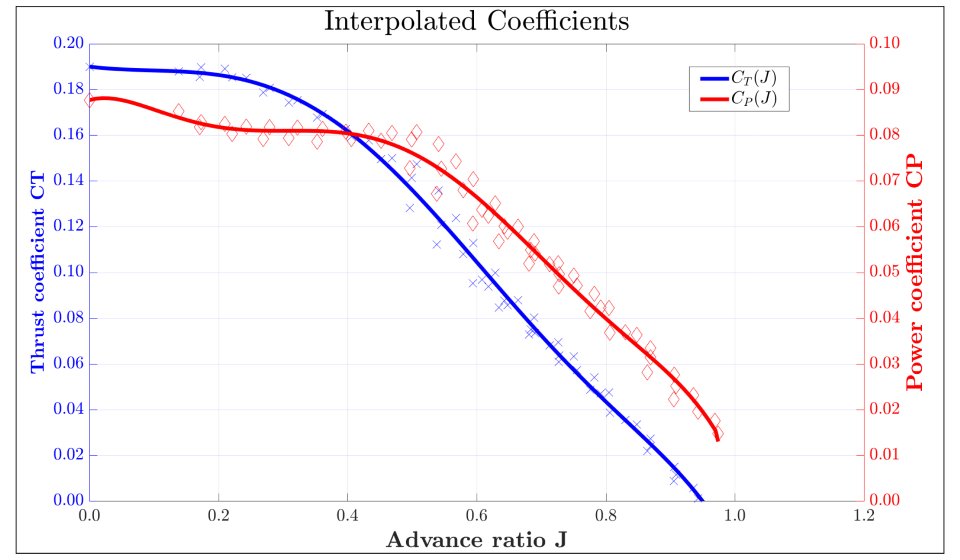
\includegraphics[width=0.5\textwidth]{graphs/coeffs-plot}
\vspace{-15pt}
\caption{Power \& thrust coefficients}
\label{fig:coeffs-plot}
\end{wrapfigure}
Where $\Omega$ is the propellers rotational speed in RPS and $D$ is the propellers diameter. For fixed pitch propellers the thrust and power coefficients are easily determined. Eq:\ref{eq:thrust-coefficient} and Eq:\ref{eq:power-coefficient} both vary due to the \emph{advance ratio} $J$.
\begin{equation}\label{eq:advance}
J = \frac{v_\infty}{\Omega R}
\end{equation}
In most cases, the net head stream velocity $v_\infty$ is the perpendicular component (projected onto the plane's normal vector $\hat{n}$) of the vehicles transnational velocity in the body frame, $\vec{v}_b\cdot\hat{n}$. For the case of a zero advance ratio, $J=0$, the conditions are regarded as static. Static thrust and power coefficients are nominal in their values. 
\end{minipage}
\par
\vspace{20pt}
\par
Propeller databases like \cite{.}\footnote{The UIUC database also includes blade profiles, pitch and chord lengths.} provide comprehensive values for a range of propeller types at different advance ratios. The introduction of those coefficients greatly simplifies the thrust estimation process. For a typical 6X4.5 inch propeller\footnote{linearly interpolated from similar pitched database results to match physical test values}, the static thrust and power coefficients respectively are:
\begin{subequations}
\begin{equation}
{\color{blue}C_{T0}}=0.19
\end{equation}
\vspace{-20pt}
\begin{equation}
{\color{red}C_{P0}}=0.12
\end{equation}
\end{subequations}
Fig:\ref{fig:coeffs-plot} shows the thrust, {\color{Blue}$C_{T}$}, and power, {\color{Red}$C_{P}$}, coefficients as a function of the advance ratio J. As the incident head fluid velocity, $v_\infty$, increases, the thrust coefficient decreases. So too does the power coefficient and hence the aerodynamic torque. 
\begin{figure}[htbp]
\begin{subfigure}{0.5\textwidth}
\centering
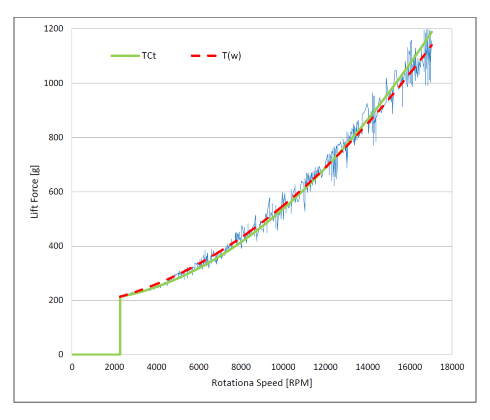
\includegraphics[width=\textwidth]{graphs/thrust-plot}
\caption{Thrust plot}
\label{fig:thrust-plot}
\end{subfigure}
\begin{subfigure}{0.5\textwidth}
\centering
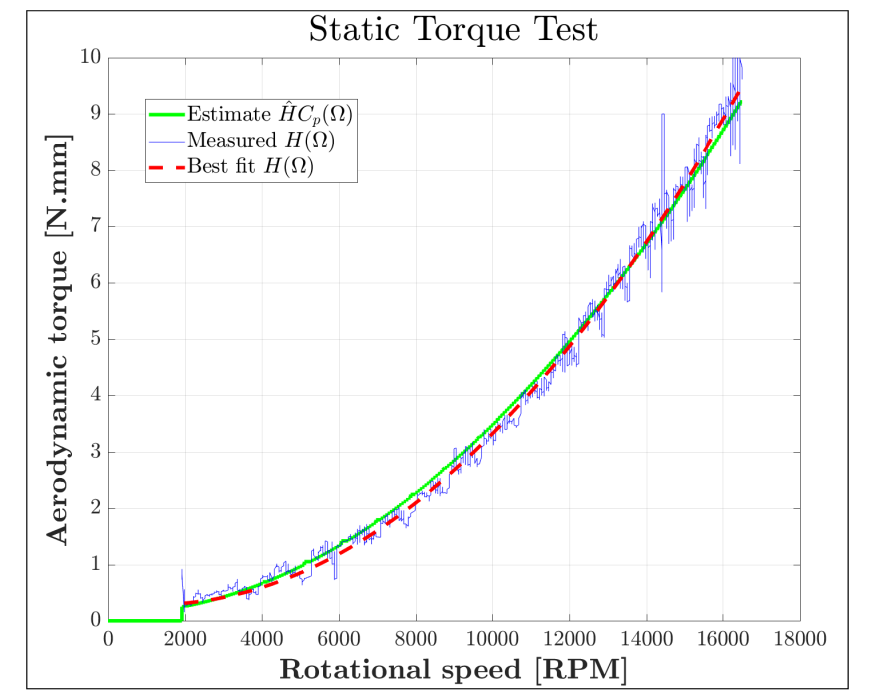
\includegraphics[width=\textwidth]{graphs/torque-plot}
\caption{Torque plot}
\label{fig:torque-plot}
\end{subfigure}
\caption{}
\label{fig:propeller-plots}
\end{figure}
In Fig:\ref{fig:propeller-plots}, the results both of static thrust and torque tests are plotted. In each test the measured values are shown (with quadratic trend-lines) and an estimated value dependent on static coefficients. Using the results from the plot in Fig:\ref{fig:coeffs-plot} as a lookup table and calculating the values from Eq:\ref{eq:coefficients}, induced propeller thrust and torques can be accurately modeled (\emph{quadratically}). Instanteous advance ratios, or rather the propeller incident fluid flow(s), are dependent on the vehicle's net transnational and angular velocity. Such that the fluid velocity's normal component to the propeller plane is given by:
\begin{equation}
v_\infty = (\vec{v}_b + \vec{L}_{arm}\times \vec{\omega}_b)\cdot \hat{n}
\end{equation}
Where $\vec{v}_b$ is the body's transnational velocity and $\vec{\omega}_b$ is the body's angular velocity, both transformed to the propeller's frame, $\in\mathcal{F}^{M_i}$. Additionally $\hat{n}$ is a unit vector normal to the propeller's rotational plane. Then $J$ is calculated as in Eq:\ref{eq:advance}.
%====================================================
\subsection{Hinged Propeller Conning \& Flapping}
\label{subsec:dynamics.aero.flap}
%====================================================
Other common non-linear aerodynamic effects which deteriorate a propellers performance are that of conning and flapping. Both effects are significantly more pronounced in the context of hinged, variable pitch propellers. The prototype under consideration here has fixed pitch, rigid propellers and as such neither conning nor propeller flapping are significant to adversely act on the system. With that being said, they are worth mentioning briefly.
\par

%====================================================
\subsection{Vortex Ring State}
\label{subsec:dynamics.aero.vrs}
%====================================================
\subsection{Drag}
\label{subsec:dynamics.aero.drag}
%====================================================

%====================================================
\section{Consolidated Model}
\label{sec:dynamics.model}%====================================================
Consolidating
%====================================================
%	CHAPTER 4 - Control
%====================================================
\chapter{Controller Development}
\label{ch:control}
%====================================================
\section{Control Loop}
\label{sec:control.loop}
%====================================================
The control problem is, as outlined in Ch:\ref{ch:intro}, to achieve non-zero setpoint tracking (for both \emph{attitude} and \emph{position} states) on a quadrotor by solving the problem of its inherent underactuation. For the intents and purposes of the subsequent controller development, the plant for some state $\vec{\mathbf{x}}$ is described in the following typical nonlinear state-space form in the time domain:
\begin{subequations}\label{eq:control-loop-states}
\begin{equation}
\frac{d}{dt}{\vec{\mathbf{x}}}=f(\vec{\mathbf{x}},t)+g(\vec{\mathbf{x}},\vec{\nu},t)
\end{equation}
\vspace{-12pt}
\begin{equation}
\vec{y} = c(\vec{\mathbf{x}},t)+d(\vec{\mathbf{x}},\vec{\nu},t)
\end{equation}
\end{subequations}
Where the plant's dynamics are governed by state progression $f(\vec{\mathbf{x}},t)$ and the plant's input response $g(\vec{\mathbf{x}},\vec{\nu},t)$ for a given control input $\vec{\nu}$. The latter could take the affine form; $g(\vec{\mathbf{x}},t)\vec{\nu}$. Setpoint tracking aims for the output to track the plant's state; namely $\vec{y} = c(\vec{\mathbf{x}},t)\equiv\vec{\mathbf{x}}$. The control problem is then to design a stabilizing control law $\mathcal{H}$ for some error state $\vec{\mathbf{x}}_e$:
\begin{equation}
\vec{\nu}_d=\mathcal{H}(\vec{\mathbf{x}}_e,\dot{\vec{\mathbf{x}}}_e,t)=\mathcal{H}(\vec{\mathbf{x}}_b,\dot{\vec{\mathbf{x}}}_b,\vec{\mathbf{x}}_d,\dot{\vec{\mathbf{x}}}_d,t)=\begin{bmatrix}
\vec{F}_d\\
\vec{\tau}_d
\end{bmatrix}
\end{equation}
Such that the controlled plant is asymptotically stabilizing or that $\lim_{t\rightarrow\infty}\vec{\mathbf{x}}_e=0$. Trajectory stability conditions are defined next in Sec:\ref{sec:control.stability}. Note that it is possible to combine attitude and position states into a single common trajectory state such that:
\\
\vspace{-5pt}
\begin{equation}
\vec{\mathbf{x}}_b=\begin{bmatrix}\vec{\mathcal{E}}_I&Q_b\end{bmatrix}^T
\end{equation}
The body's trajectory is then fully described by $\vec{\mathbf{x}}_b(t)$. Separate control laws are developed for attitude and position tracking and hence those states are not combined in the context of this control project. However for the purposes of describing the control plant, a single major loop control is structure considered.
\par
Because of the plant's overactuatedness the control loop is split into two blocks; first a higher level \emph{setpoint tracking} controller designs a virtual control input $\vec{\nu}_d$. That being net forces $\vec{F}_d$ and torques $\vec{\tau}_d$ to act on the body. A lower level \emph{allocator} then solves for explicit actuator positions from $\vec{\nu}_d$ to physically actuate that \emph{virtual} control input. The actuator set then implements a commanded control input $\vec{\nu}_c$ through its effectiveness function (Eq:\ref{eq:dynamic-plant-inputs}) with an actuator estimate $\hat{u}$ subject to transfer functions $C(s)$:
\begin{equation}\label{eq:control-effectiveness}
\vec{\nu}_c=B(\vec{\mathbf{x}},\hat{u},t)=\begin{bmatrix}
\vec{F}_c(u) & \vec{\tau}_c(u)
\end{bmatrix}^T
\end{equation}
The allocator solves for commanded actuator values $u_c$ such that $\vec{\nu}_c\rightarrow\vec{\nu}_d$. That allocation function, $B^\dagger$, can be \emph{roughly} referred to as the effectiveness inverse:
\begin{equation}
u_c=B^{\dagger}(\vec{\mathbf{x}},\vec{\nu}_d,t)~~~~\in\mathbb{U}
\end{equation}
This chapter derives higher level controllers for $\vec{\nu}_d=\mathcal{H}(\vec{\mathbf{x}}_e,\dot{\vec{\mathbf{x}}}_e,t)$; allocation rules are discussed next in Ch:\ref{ch:allocation}. A collection of attitude and position controllers are presented here whose stability is proven with Lyapunov theorem \cite{bojelayupanov,lyapunovstabilitytheorem,noteonlyapunov}. Each controller is compared in the context of an overactuated quadrotor plant, similarly a series of allocation schemes are presented. For the most part, it is assumed errors between commanded actuator setpoints $u$ and their state estimates $\hat{u}$ affected by transfer functions $C(s)$ are negligible. That plant dependent error is small and diminishing over time but is later incorporated into adaptive control in Sec:\ref{subsubsec:control.attitude.nonlinear.adaptivebackstep}. Resultant controller comparisons, their details and efficacy are evaluated subsequently in Ch:\ref{ch:simulation}. 
\par
A generalized overactuated control loop consists of a series of cascaded control blocks (Fig:\ref{fig:control-loop}). From the trajectory's error state $\vec{\mathbf{x}}_e$, a control law designs a virtual control input $\vec{\nu}_d$ which is applied to the allocation block. The allocation law $B^{\dagger}(\vec{\mathbf{x}},\vec{\nu}_d,t)$ solves for physical actuator positions $u_c\in\mathbb{U}$. Commanded actuator (\emph{estimate}) positions affect a physical input $\vec{\nu}_c=B(\vec{\mathbf{x}},\hat{u},t)$ which is an input applied to the state's dynamics, Eq:\ref{eq:control-loop-states}. Finally the output tracking state is estimated with some filter paradigm $\hat{\mathbf{x}}=A(\vec{\mathbf{x}},t)$ which is fed back for error state calculation (Sec:\ref{sec:simulation.state}).
\begin{figure}[htbp]
\centering
\includegraphics[width=0.97\textwidth]{figs/control-loop}
\vspace{-28pt}
\caption{Generalized control loop with allocation}
\vspace{-16pt}
\label{fig:control-loop}
\end{figure}
\par
Fig:\ref{fig:control-loop} shows a generalized overactuated control loop's structure; the plant's dynamics from Eq:\ref{eq:quaternion-states} include state derivative feedback. Moreover aspects of the state transfer function includes multibody nonlinearities dependent on actuator positions and rates as detailed in Sec:\ref{sec:dynamics.nonlinearities}. That generalized case is now refined in the context of an overactuated quadcopter.
%====================================================
\section{Control Plant Inputs}
\label{sec:control.inputs}
%====================================================
Control inputs for the differential state equations, from Eq:\ref{eq:quaternion-states}, have mostly been described with net forces and torques; $\vec{F}_\mu(\hat{u})$ and $\vec{\tau}_\mu(\hat{u})$. The relationship of the \emph{effectiveness function} between each propeller's rotational speed and servo positions with the produced thrust vector is calculated from Eq:\ref{eq:quaternion-inputs}.
\begin{subequations}\label{eq:control-input}
\begin{equation}
\vec{\nu}_c\triangleq\begin{bmatrix}
\vec{F}_\mu(\hat{u}) & \vec{\tau}_\mu(\hat{u})
\end{bmatrix}^T=B(\vec{\mathbf{x}},\hat{u},t)~~~~\in\mathbb{R}^6,~u\in\mathbb{U}
\end{equation}
\vspace{-10pt}
\begin{equation}
\vec{F}_\mu(\hat{u})=\sum_{i=1}^4 Q_{M_i}^*(\lambda_i,\alpha_i)\otimes \vec{T}(\Omega_i)\otimes Q_{M_i}(\lambda_i,\alpha_i)~~~~\in\mathcal{F}^b
\end{equation}
\vspace{-4pt}
\begin{equation}
\vec{\tau}_\mu(\hat{u})=\sum_{i=1}^4 \vec{L}_i\times\big(Q_{M_i}^*(\lambda_i,\alpha_i)\otimes \vec{T}(\Omega_i)\otimes Q_{M_i}(\lambda_i,\alpha_i)\big)~~~~\in\mathcal{F}^b
\end{equation}
\end{subequations}
As mentioned previously, a higher level controller $\mathcal{H}(\vec{\mathbf{x}}_e,\dot{\vec{\mathbf{x}}}_e,t)$ designs desired net plant inputs $\vec{\nu}_d=\begin{bmatrix}\vec{F}_d&\vec{\tau}_d\end{bmatrix}^T$ whilst a lower level allocator commands actuator positions $u_c=B^{\dagger}(\vec{\mathbf{x}},\vec{\nu}_d,t)$. This separation allows for independent comparison of proposed control and allocation laws. However, typical allocation rules like pseudo-inversion require an affine relationship between plant and control inputs, detailed in Sec:\ref{subsubsec:intro.lit.control.allocation}).
\par
The relationship in Eq:\ref{eq:control-input} is not reducible to a single multiplicative relationship with the actuator matrix $u\in\mathbb{U}$. So the effectiveness function needs an extra layer of abstraction to incorporate a multiplicative relationship. Rather than calculating explicit actuator positions directly from $\vec{\nu}_d$; a set of four 3-D thrust vectors $\vec{T}_{1\rightarrow 4}$ for each motor module are first calculated.
\begin{subequations}\label{eq:4.7}
\begin{equation}
\vec{\nu}_c=\begin{bmatrix}
\vec{F}_c(u)\\
\vec{\tau}_c(u)
\end{bmatrix}
= 
\begin{bmatrix}
\mathbb{I}_{3\times 3} & \mathbb{I}_{3\times 3} & \mathbb{I}_{3\times 3} & \mathbb{I}_{3\times 3}\\
[\vec{L}_1]_\times & [\vec{L}_2]_\times & [\vec{L}_3]_\times & [\vec{L}_4]_\times
\end{bmatrix}
\begin{bmatrix}
\vec{T}_1&
\vec{T}_2&
\vec{T}_3&
\vec{T}_4
\end{bmatrix}^T
\end{equation}
\begin{equation}
\rightarrow\vec{\nu}_c=B'(\vec{\mathbf{x}},t)\begin{bmatrix}
\vec{T}_1&
\vec{T}_2&
\vec{T}_3&
\vec{T}_4
\end{bmatrix}^T
\end{equation}
\end{subequations}
Where $[\vec{L}_i]_\times$ is the cross product vector of the $i^{th}$ torque arm from Eq:\ref{eq:cross-product-matrix}. Explicit actuator positions for each module, $[\Omega_i,\lambda_i,\alpha_i]^T$, can then be solved from those thrust vectors $\vec{T}_i$ for $i\in[1:4]$ with some trigonometry, ``undoing" the transformation applied in Eq:\ref{eq:control-input}. That trigonometric inversion is detailed later in Sec:\ref{sec:allocation.inversion} but is described as the function $R^\dagger$:
\begin{equation}\label{eq:4.8}
[\Omega_i,~\lambda_i,~\alpha_i]^T=R^\dagger(\vec{\mathbf{x}},\vec{T}_i,t)~~~~\text{for}~i\in[1:4]
\end{equation}
The generalized control loop illustrated in Fig:\ref{fig:control-loop} is extended to include the abstracted allocation blocks of Eq:\ref{eq:4.7} and Eq:\ref{eq:4.8}, shown in Fig:\ref{fig:control-block}. The net control block still solves for the same actuator matrix $u\in\mathbb{U}$. The entire loop accommodates for comparison of various $B^\dagger(\vec{\mathbf{x}},\vec{\nu}_d,t)$ allocation rules without having to redesign the remainder of the loop's structure.
\begin{figure}[htbp]
\vspace{-8pt}
\centering
\includegraphics[width=\textwidth]{figs/control-block}
\caption{Extended control loop with overactuation}
\label{fig:control-block}
\vspace{-16pt}
\end{figure}
\par
Certain blocks in Fig:\ref{fig:control-block} use actuator estimates $\hat{u}$ to calculate responses for feedback compensation, other blocks are affected by instantaneous actuator positions $u$. The two are, for the most part, interchangeable as minor loop transfer dynamics of $C(s)$ in Sec:\ref{subsec:proto.design.transfer}. In summary; each controller designs a net force and torque to act on the body. Allocation rules decompose that virtual input into four separate 3-D thrust vectors, or twelve directional components. The force components are an abstracted allocation layer in place of explicit actuator positions, which are subsequently solved for\ldots
\begin{equation}
B^{\dagger}(\mathbf{x},\vec{\nu}_d,t)=\big[ T_{1x},~T_{1y},~T_{1z},~\ldots~T_{4x},~T_{4y},~T_{4z}\big]^T
\end{equation}
Each control law is co-dependent on an accompanying allocation algorithm. Traditional control loops (underactuated or well matched) typically have a unity allocation rule and as such require no consideration so they're mostly disregarded. Separate control laws for attitude ad position control are presented in Section:\ref{sec:control.attitude} and \ref{sec:control.position} respectively. Thereafter a series of allocation rules are proposed in Ch:\ref{ch:allocation}. Although presented independently, the controller and allocation laws are mutually inclusive. The stability of each controller is proven objectively but explicit controller coefficients are optimized in the subsequent Ch:\ref{ch:simulation}, in Sec:\ref{sec:simulation.tuning}.
\newpage
%====================================================
\section{Stability}
\label{sec:control.stability}
%====================================================
Before undertaking the control plant derivations, it is worth outlining definitions of the control objective's stability. The research question aims to achieve non-zero setpoint tracking of state's trajectory. A control loop then aims to \emph{stabilize} the dynamics described previously in Sec:\ref{sec:dynamics.model} whilst tracking particular trajectories for attitude and position setpoints, $\vec{\mathbf{x}}_d(t)=[\vec{\mathcal{E}}_d(t)~Q_d(t)]^T$. 
\par
The entire system's control loop was previously detailed in Sec:\ref{sec:control.loop}. Stability in the context of trajectory tracking must first be defined. Generalized trajectory stability definitions are not uncommon in the context of energy based control design, or Lyapunov theorem (Sec:\ref{sec:control.lyapunov}). Stability definitions pertinent to Lyapunov's stability theorem are briefly presented here; the following is adapted from \cite{bojelayupanov,lyapunovstabilitytheorem}. In general for some autonomous trajectory $\vec{\mathbf{x}}(t)$, an equilibrium point $\vec{\mathbf{x}}(t_0)$ is said to be stable (\textbf{S}) if and only if (\emph{iff}) the following is true:
\begin{subequations}\label{eq:basic-stability}
\begin{equation}
\forall\varepsilon>0,~\exists~\delta_0(t_0,\varepsilon):~\norm{\vec{\mathbf{x}}(t_0)}<\delta_0(t_0,\varepsilon)
\end{equation}
\vspace{-20pt}
\begin{equation}
\Rightarrow\norm{\vec{\mathbf{x}}(t)}<\varepsilon,~~\forall t\geq t_0
\end{equation}
\end{subequations}
The implication of which is that if, for some initial condition $\vec{\mathbf{x}}(t_0)$ whose magnitude is bound by the manifold $\delta_0(t_0,\varepsilon)$, the entire subsequent trajectory of $\vec{\mathbf{x}}(t)$ is bound from above by some other manifold $\varepsilon$. Basic stability is illustrated in Fig:\ref{fig:basic-stability} for a 2-D trajectory.
\begin{figure}[hbtp]
\vspace{-6pt}
\centering
\begin{subfigure}{0.49\textwidth}
\centering
\includegraphics[width=\textwidth]{figs/basic-stability}
\vspace{-16pt}
\caption{Basic stability}
\label{fig:basic-stability}
\end{subfigure}
\begin{subfigure}{0.49\textwidth}
\centering
\includegraphics[width=\textwidth]{figs/uniform-stability}
\vspace{-16pt}
\caption{Uniform stability}
\label{fig:uniform-stability}
\end{subfigure}
\vspace{-8pt}
\caption{Trajectory illustrations for $\mathbf{S}$ and $\mathbf{US}$}
\vspace{-18pt}
\end{figure}
\par
An equilibrium point is further said to be uniformly stable (\textbf{US}) \emph{iff} for the time $t\in[t_0,\infty)$ the following criteria, being an extension of basic stability, is met:
\begin{subequations}\label{eq:uniform-stability}
\begin{equation}
\forall\varepsilon>0,~\exists~\delta_0(\varepsilon)>0:~\norm{\vec{\mathbf{x}}(t_1)}<\delta_0(\varepsilon),~~t_1>t_0
\end{equation}
\vspace{-18pt}
\begin{equation}
\Rightarrow\norm{\vec{\mathbf{x}}(t)}<\varepsilon,~~\forall
t\geq t_1
\end{equation}
\end{subequations}
\textbf{US} similarly bounds a trajectory from above by $\varepsilon$ if the trajectory originates from within $\delta_0(\varepsilon)$. The difference is that the principle trajectory region $\delta_0(\varepsilon)$ is independent of $t_0$ in the case of \textbf{US}. The two surfaces are non-concentric; a $\mathbf{US}$ trajectory is illustrated in Fig:\ref{fig:uniform-stability}. Uniform stability is a subset of general stability, $\mathbf{US}\subset\mathbf{S}$, however the converse is not true. Furthermore \textbf{US} is a stronger qualification of stability, each subsequent stability presented represents a stronger assertion of stability.
\par
Extending stability definitions to include settling; an equilibrium point is said to be asymptotically stable (\textbf{AS}) \emph{iff} conditions for \textbf{S} are met (Eq:\ref{eq:basic-stability}) and that the following holds true:
\begin{subequations}\label{eq:asymptotic-stability}
\begin{equation}
\exists~\delta_1(t_0,\varepsilon) >0:~\norm{\vec{\mathbf{x}}(t_0)}<\delta_1(t_0,\varepsilon)
\end{equation}
\vspace{-18pt}
\begin{equation}
\Rightarrow \lim_{t\rightarrow\infty}\norm{\vec{\mathbf{x}}(t)}\rightarrow 0
\end{equation}
\end{subequations}
This asserts that trajectories originating within some finer region $\delta_1(t_0,\varepsilon)$, being a subset of $\delta_0(t_0,\varepsilon)$, tends to and \emph{asymptotically} settles at the origin. In the case of \textbf{AS} the origin is both \emph{stable} and \emph{attractive} (shown in Fig:\ref{fig:asymptotic-stability}). Asymptotic stability is typically the first requirement for any control law, being a stronger stability than both \textbf{US} and \textbf{S}, typically stabilizing a control setpoint's error\ldots
\begin{figure}[hbtp]
\centering
\begin{subfigure}{0.49\textwidth}
\centering
\includegraphics[width=\textwidth]{figs/asymptotic-stability}
\vspace{-8pt}
\caption{Asymptotic stability}
\label{fig:asymptotic-stability}
\end{subfigure}
\begin{subfigure}{0.49\textwidth}
\centering
\includegraphics[width=\textwidth]{figs/uniform-asymptotic-stability}
\vspace{-8pt}
\caption{Uniform asymptotic stability}
\label{fig:uniform-asymptotic-stability}
\end{subfigure}
\vspace{-4pt}
\caption{Trajectory illustrations for $\mathbf{AS}$ and $\mathbf{UAS}$}
\vspace{-14pt}
\end{figure}
\par
Uniform asymptotic stability (\textbf{UAS}), an extension of asymptotic stability $\mathbf{UAS}\subset\mathbf{AS}$, occurs when the asymptotically stable bound region $\delta_1(\epsilon)$ is independent of the principle starting $t_0$. An equilibrium point is \textbf{UAS} \emph{iff} conditions for \textbf{S} are met and that:
\begin{subequations}\label{eq:uniform-asymptotic-stability}
\begin{equation}
\exists~\delta_1(\varepsilon)>0:~\norm{\vec{\mathbf{x}}(t_1)}<\delta_1(\varepsilon),~~t_1\geq t_0
\end{equation} 
\vspace{-16pt}
\begin{equation}
\Rightarrow \lim_{t\rightarrow\infty}\norm{\vec{\mathbf{x}}(t)}\rightarrow 0
\end{equation}
\end{subequations}
A uniformly asymptotic equilibrium point implies stability from a non-concentric ball of attraction; settling to the origin (illustrated in Fig:\ref{fig:uniform-asymptotic-stability}). 
\par
An equilibrium point is regarded as exponentially stable (\textbf{UES}) if conditions for \textbf{UAS} are met and that there exist $\exists~a,b,r$ that bound the settling of the trajectory such that:
\begin{equation}\label{eq:exponential-stability}
\norm{\vec{\mathbf{x}}(t,t_0,\vec{\mathbf{x}}_0)}\leq a\norm{\vec{\mathbf{x}}_0}e^{-bt},~~\forall\norm{\vec{\mathbf{x}}_0}\leq r
\end{equation}
The term $a\norm{\vec{\mathbf{x}}_0}e^{-bt}$ bounds the rate at which the trajectory settles to the origin, illustrated in Fig:\ref{fig:exponential-stability}. The initial point of the trajectory, $\vec{\mathbf{x}}_0$ is bound from above by some $r\triangleq \delta_1(\varepsilon)$. Moreover uniform stability is \emph{implied} with exponential stability.
\begin{figure}[hbtp]
\centering
\begin{subfigure}{0.49\textwidth}
\includegraphics[width=\textwidth]{figs/exponential-stability}
\vspace{-14pt}
\caption{Exponential stability}
\label{fig:exponential-stability}
\end{subfigure}
\begin{subfigure}{0.49\textwidth}
\centering
\includegraphics[width=\textwidth]{figs/global-exponential-stability}
\vspace{-14pt}
\caption{Global exponential stability}
\label{fig:global-exponential-stability}
\end{subfigure}
\vspace{-4pt}
\caption{Trajectory illustrations for \textbf{UES} and \textbf{GUES}}
\vspace{-14pt}
\end{figure}
\par
The above definitions of stabilities are only locally defined, and so the stabilities hold true only for local trajectories, only in the case of $\vec{\mathbf{x}}(t_0)\leq\varepsilon$. Extending \textbf{UAS} to global uniform asymptotic stability (\textbf{GUAS}); the origin's equilibrium point is \textbf{GUAS} \emph{iff} conditions for \textbf{UAS} are first met, the origin is only the equilibrium point and the asymptotic approach can be extended such that:
\begin{subequations}
\begin{equation}
\exists~\delta_1(\varepsilon)>0:~\norm{\vec{\mathbf{x}}(t_1)}<\delta_1(\varepsilon),~~t_1\geq t_0
\end{equation}
\vspace{-16pt}
\begin{equation}
\Rightarrow \lim_{t\rightarrow\infty}\norm{\vec{\mathbf{x}}(t)}\rightarrow 0,~~\forall \vec{\mathbf{x}}(t_0)
\end{equation}
\end{subequations}
Similarly exponential stability can extend to the global case, shown in Fig:\ref{fig:global-exponential-stability}, but only \emph{iff} \textbf{UES} conditions are first met. In the global case, the origin can be the \emph{only equilibrium point}. Stability from Eq:\ref{eq:exponential-stability} is then globally:
\begin{equation}\label{eq:global-exponential-stability}
\norm{\vec{\mathbf{x}}(t,t_0)}\leq a\norm{\vec{\mathbf{x}}_0}e^{-bt},~~\forall\norm{\vec{\mathbf{x}}_0}
\end{equation}
Initial trajectory conditions are dropped in Eq:\ref{eq:global-exponential-stability}, for any number of trajectories until $\vec{\mathbf{x}}_n(t)$; each trajectory is bound by an exponential $a_n\norm{\vec{\mathbf{x}}_t(0)}e^{-b_nt}$. It follows that, irrespective of the starting point $\vec{\mathbf{x}}_n(t_0)$ for the trajectory, the system \emph{always} settles to the origin. \textbf{GUES} is the strongest sense of stability and provides insight into the trajectory stabilizing rate. The most desirable control design outcome is a controller which applies globally uniform exponential stability to a plant.
%====================================================
\section{Lyapunov Stability Theorem}
\label{sec:control.lyapunov}
%====================================================
Lyapunov's stability theory is an important aspect of nonlinear controller design. An abundance of literature exists on the subject, included in almost every meritable textbook or control paper. If the reader is unfamiliar with Lyapunov's theorem,  \cite{noteonlyapunov,nonlinearsystems,bojelayupanov} each explains the concept in detail. The following is adapted from \cite{bojelayupanov} and \cite{lyapunovstabilitytheorem} and briefly outlines how Lyapunov's stability theorem is used to prove (\emph{global}) asymptotic stability for continuous time invariant systems, linear or otherwise. The theory analyzes a generalized energy function of a system's autonomous trajectory. If the trajectory has a negative energy derivative that implies the system's energy will always dissipate towards a state of zero energy or stable equilibrium point. Lyapunov analysis is a powerful tool for stability verification because the system's trajectory itself need not be explicitly defined for stability to be determined. Proof of Lyapunov's theorem is done with a contradiction disproof and, as such, the theoretical underpinning is somewhat cumbersome.
\par
It is worth reiterating its fundamentals given that backstepping controllers are proposed later in Sec:\ref{subsec:control.attitude.nonlinear} for attitude control. A backstepping controllers enforce Lyapunov stability criteria onto the system through interative control structure design, \cite{backstepping,adaptivebackstep,intelligentbackstep}. In general, given a nonlinear time invariant system that follows some continually differentiable trajectory $\vec{\mathbf{x}}(t)$, typically the trajectory is going to progress subject to some rule:
\begin{equation}\label{eq:4.17}
\dot{\vec{\mathbf{x}}}(t)=f\big(\vec{\mathbf{x}}(t),u\big)
\end{equation}
Then, constructing a generalized positive-definite function generalized energy or \emph{Lyapunov function candidate} (\emph{LFC}) $V(\vec{\mathbf{x}})$ for a trajectory $\vec{\mathbf{x}}(t)$. A positive definite matrix $M$ is defined such that:
\begin{equation}
\mathbf{z}^TM\mathbf{z}\geq 0~~~\forall \mathbf{z}
\end{equation}
As such an LFC typically, but not exclusively, has the quadratic and positive-definite form with some positive square matrix $P\in\mathbb{R}^{n\times n}>0$:
\begin{equation}
V(\vec{\mathbf{x}})=\vec{\mathbf{x}}\hspace{1pt}^TP\vec{\mathbf{x}},~~\vec{\mathbf{x}}\in\mathbb{R}^{n}
\end{equation}
An LFC could simply be positive semi-definite over the trajectory's path, the quadratic form is just convenient for the use of backstepping. From its definition the trajectory Eq:\ref{eq:4.17} is continually differentiable; there is then a gradient matrix for each element of $V(\vec{\mathbf{x}})$ in the form:
\begin{equation}\label{eq:4.20}
\nabla V(\vec{\mathbf{x}})\triangleq\bigg[\frac{\partial V(\vec{\mathbf{x}})}{\partial x_1}~\frac{\partial V(\vec{\mathbf{x}})}{\partial x_2}~\ldots~\frac{\partial V(\vec{\mathbf{x}})}{\partial x_n}\bigg]~~~~\vec{\mathbf{x}}\in\mathbb{R}^n
\end{equation}
The energy function's derivative, otherwise referred to as the \emph{Lie derivative} in some texts;\cite{noteonlyapunov,nonlinearsystems}, is calculated from partial derivatives in Eq:\ref{eq:4.20} as follows:
\begin{equation}
\dot{V}(\vec{\mathbf{x}})\triangleq\nabla V(\vec{\mathbf{x}})^T\frac{d}{dt}f(\vec{\mathbf{x}})=\frac{\delta V(\vec{\mathbf{x}})}{\delta x_1}\frac{df_1(x_1)}{dt}+\frac{\delta V(\vec{\mathbf{x}})}{\delta x_2}\frac{df_2(x_2)}{dt}+~\ldots~+\frac{\delta V(\vec{\mathbf{x}})}{\delta x_n}\frac{df_n(x_b)}{dt}
\end{equation}
Lyapunov's theorem states that \emph{iff} the candidate function $V(\vec{\mathbf{x}})$ is positive definite with $V(\vec{0})=0$ and its derivative is strictly negative; $\dot{V}(\vec{\mathbf{x}})< 0~~\forall \vec{\mathbf{x}}(t) \not= 0$, the system is then asymptotically stable ($\mathbf{AS}$ from Eq:\ref{eq:asymptotic-stability}). Mathematically that means, for any $\vec{\mathbf{x}}(t)$ with $t\geq t_0$:
\begin{equation}\label{eq:4.22}
V\big(\vec{\mathbf{x}}(t)\big)=V\big(\vec{\mathbf{x}}(t_0)\big)+\int_{t_0}^t \dot{V}\big(\vec{\mathbf{x}}(t)\big).dt \leq V\big(\vec{\mathbf{x}}(t_0)\big)
\end{equation}
Which can be physically interpreted as the system's generalized energy function dissipating, irrespective of the trajectory path taken. With a strictly decreasing energy function, the system will stabilize to a state of zero energy which, naturally, is a stable equilibrium point.
\begin{equation}
\lim_{t\rightarrow\infty}\norm{V\big(\vec{\mathbf{x}}(t)\big)}\rightarrow 0
\end{equation}
The trajectory's asymptotic stability can be extended to exponential stability boundedness, such that \emph{iff} the same conditions are met for asymptotic stability in Eq:\ref{eq:4.22} and there exists some positive coefficient $\alpha>0$ such that $\dot{V}(\vec{\mathbf{x}})\leq-\alpha V(\vec{\mathbf{x}})$. That implies the system is globally exponentially stable as is bound in such a way that:
\begin{equation}
\norm{V\big(\vec{\mathbf{x}}(t)\big)}\leq Me^{-\alpha t/2}\norm{V\big(\vec{\mathbf{x}}(t_0)\big)}
\end{equation}
%====================================================
\section{Model Dependent \& Independent Controllers}
%====================================================
Two classes of controllers are included for a full state trajectory tracking control loop; both attitude and position control laws. Attitude setpoint tracking is the primary focus of this research project (Sec:\ref{subsec:control.attitude.problem}) and incorporates a more detailed schedule of controller design and evaluation. 
\par
The allocation law combines both virtual control inputs from attitude and position controllers, $\vec{\nu}_d=[\vec{F}_d~\vec{\tau}_d]^T$, to solve for explicit actuator positions. Controller dependency on the plant's state is as a consequence of the actuator responses and complex inertial dynamics, as derived previously in Sec:\ref{subsec:dynamics.nonlinearities.gyrotorques}. Whilst not a prerequisite for stability, plant dependent compensation obviously improves controller performances. Independent and dependent cases are only considered for one type of controller; the most basic case proportional-derivative controller in Section:\ref{subsubsec:control.attitude.controllers.pd} and tested in Sec:\ref{subsec:simulation.attitude.pd}. All other control laws compensate for unwanted plant dynamics in a feedback configuration.
\par
The plant dependency makes backstepping controllers an effective controller choice for this dissertation's context. The proposed plant dependent control laws compensate for undesirable dynamics their design, basic PD and PID control structures (\emph{and the like}) will not. The first and most basic control solution, used as a reference case, is a PD controller for attitude and position with direct-inversion (Pseudo or Moore-Penrose inversion) allocation. 
%====================================================
\section{Attitude Control}
\label{sec:control.attitude}
%====================================================
\subsection{The Attitude Control Problem}
\label{subsec:control.attitude.problem}
%====================================================
The setpoint tracking control problem (\cite{attitudecontrolproblem}) for the attitude plant is to design a stabilizing control torque $\vec{\tau}_d=h(\vec{\mathbf{x}}_e,\dot{\vec{\mathbf{x}}}_e,t)$ such that for any desired attitude quaternion $\forall~Q_d\in\mathbb{Q}$ and an instantaneous attitude body quaternion $Q_b\in\mathbb{Q}$ the error state asymptotically stabilizes to the origin; $Q_e\rightarrow[1~\vec{0}~]^T$. Or that:
\begin{equation}
\vec{\tau}_d=h(Q_d,~\dot{Q}_d,~Q_b,~\dot{Q}_b)~~\text{such that}~~\underset{t\rightarrow\infty}{\lim}Q_b\rightarrow Q_d
\end{equation}
Quaternion attitude error states are defined as the Hamilton product or \emph{difference} between the desired and instantaneous quaternion attitude states, previously in Eq:\ref{eq:quaternion-error}. Quaternion error states are multiplicative, in contrast with the subtractive relationship for Euler angle error states. The attitude error state is defined as:
\begin{equation}\label{eq:quaternion-error-control}
Q_e\triangleq Q_b^*\otimes Q_d
\end{equation}
The relative angular velocity error between the body frame $\mathcal{F}^b$ and the trajectory's desired frame $\mathcal{F}^d$ is given as $\vec{\omega}_e$. The body angular velocity $\vec{\omega}_b$ is subject to the differential Eq:\ref{eq:quaternion-states-angular}. As such there is an angular rate error:
\begin{subequations}
\begin{equation}\label{eq:angular-error}
\vec{\omega}_e\triangleq\vec{\omega}_d-\vec{\omega}_b\hspace{-2pt}'~~~~\in\mathcal{F}^d
\end{equation}
The desired angular velocity $\vec{\omega}_d$ is taken with respect to the desired angular attitude frame, and so it must be transformed back onto the existing body frame.
\begin{equation}
\vec{\omega}_e=Q_e^*\otimes\vec{\omega}_d\otimes Q_e-\vec{\omega}_b~~~~\in\mathcal{F}^{b}
\end{equation}
Typically for the trajectories generated here only first order setpoints are commanded, hence the desired angular velocity is zero; $\vec{\omega}_d=\vec{0}$. It follows that the angular rate error is then simply the negative body angular velocity. It would be easy to incorporate a non-zero angular velocity setpoints to accommodate for higher order state derivative tracking trajectories.
\begin{equation}\label{eq:4.27c}
\vec{\omega}_e=-\vec{\omega}_b\Big|_{\vec{\omega}_d=\vec{0}}
\end{equation}
\end{subequations}
The time derivative for the quaternion error state is calculated from the quaternion derivative definition Eq:\ref{eq:quaternion-deriv}. The derivative $\dot{Q}_e$ is then dependent on the angular velocity error and calculated as follows:
\begin{equation}
\dot{Q}_e=\frac{1}{2}Q_e\otimes\vec{\omega}_e=-\frac{1}{2}Q_e\otimes\vec{\omega}_b\Big|_{\vec{\omega}_d=\vec{0}}
\end{equation}
%====================================================
\subsection{Linear Controllers}
\label{subsec:control.attitude.controllers}
%====================================================
\subsubsection{PD Controller}
\label{subsubsec:control.attitude.controllers.pd}
%====================================================
The following control law is used as a reference case for comparing the remaining controllers derived. It is a simple proportional-derivative (\emph{PD}) attitude controller, adapted from \cite{fullquaternion} and following a stability proof similar to the one derived in \cite{attitudecontrolproblem}. An attitude PD controller is proportional only to the \emph{vector quaternion error}. Such that the error is the same dimension as the angular velocity error; $\vec{q}_e\in\mathbb{R}^3$. A PD controller designs the commanded torque input:
\begin{equation}\label{eq:independent-pd}
\vec{\tau}_{_{PD}}=K_d\vec{\omega}_e+K_p\vec{q}_e~~~~\in\mathcal{F}^b
\end{equation}
Where both $K_d$ and $K_p$ are \emph{positive symmetrical} $3\times 3$ gain coefficient matrices to be determined at a later stage. Eq:\ref{eq:independent-pd} neglects the quaternion scalar error and is therefore susceptible to unwinding. Using a positive-definite Lyapunov function candidate $V_{_{PD}}$ for the attitude trajectory:
\begin{equation}\label{eq:lyapunov-pd}
V_{_{PD}}(Q_e,\vec{\omega}_e)=\vec{q}_e\text{}^T\vec{q}_e+(1-q_0)^2+\frac{1}{2}\vec{\omega}_e\text{}^TJ_b(u)K_p^{-1}\vec{\omega}_e~~>0,~\forall(Q_e,\vec{\omega}_e)
\end{equation}
Note also that $V_{_{PD}}([\pm 1~\vec{0}\hspace{1pt}]^T,\vec{0}\hspace{1pt})=0$, making it a suitable LFC. Exploiting the unit quaternion's inherent magnitude property, it follows that:
\begin{equation}\label{eq:4.171}
\norm{Q}=\vec{q}\text{}^{\hspace{3pt}T}\vec{q}+q_0\text{}^2=\vec{q}\text{}^{\hspace{3pt}2}+q_0\text{}^2=1
\end{equation}
Substituting that and the angular velocity's error state, $\vec{\omega}_e=-\vec{\omega}_b$; the proportional derivative LFC in Eq:\ref{eq:lyapunov-pd} reduces to:
\begin{subequations}\label{eq:4.18}
\begin{equation}
V_{_{PD}}=\vec{q}_e\text{}^2+\big(q_0\text{}^2 -2q_0 + 1\big) +\frac{1}{2}\vec{\omega}_e\text{}^TJ_b(u)K_p^{-1}\vec{\omega}_e
\end{equation}
\vspace{-10pt}
\begin{equation}
=2(1-q_0)+\frac{1}{2}\vec{\omega}_b\text{}^TJ_b(u)K_p^{-1}\vec{\omega}_b\Big|_{\vec{\omega}_e=-\vec{\omega}_b}
\end{equation}
\end{subequations}
Taking the derivative of that Lyapunov Function candidate then yields:
\begin{equation}\label{eq:lyapunov-pd-deriv}
\dot{V}_{_{PD}}(\vec{q}_e,\vec{\omega}_e)=-2\dot{q}_0+\vec{\omega}_b\text{}^TJ_b(u)K_p^{-1}\dot{\vec{\omega}}_b
\end{equation}
Recalling the angular velocity differential equation from Eq:\ref{eq:quaternion-states-angular}, $\dot{\vec{\omega}}_b$ with a control torque input $\vec{\tau}_{_{PD}}$ from Eq:\ref{eq:independent-pd}:
\begin{equation}
\dot{\vec{\omega}}_b=J_b\text{}^{-1}(u)\big(-\vec{\omega}_b\times J_b(u)\vec{\omega}_b-\vec{\tau}_b(u)+\vec{\tau}_g+\vec{\tau}_H+\vec{\tau}_{_{PD}}\big)~~~~\in\mathcal{F}^b
\end{equation}
Where $\vec{\tau}_H$ is a simplified representation of the net aerodynamic torque experienced by the body from the rotating propellers, from Eq:\ref{eq:consolidated-h-torque}. Then, using the fact that a quaternion's derivative by definition is:
\begin{equation}\label{eq:quat-derivative}
\dot{Q}=\begin{bmatrix}
-\frac{1}{2}\vec{q}^{\hspace{3pt}T}\vec{\omega}\\
\frac{1}{2}\big([\vec{q}\hspace{3pt}]_\times+q_0\mathbb{I}_{3\times 3}\big)\vec{\omega}
\end{bmatrix}
\end{equation}
Substituting the above into the LFC derivative $\dot{V}_{_{PD}}$ in Eq:\ref{eq:lyapunov-pd-deriv} with an expanded $\vec{\tau}_{_{PD}}$ yields:
\begin{subequations}
\begin{equation}
\rightarrow\dot{V}_{_{PD}}=\vec{q}_e\text{}^T\vec{\omega}_e+\vec{\omega}_b\text{}^TJ_b(u)K_p^{-1}\Big(J_b(u)^{-1}\big(-\vec{\omega}_b\times J_b(u)\vec{\omega}_b-\vec{\tau}_b+\vec{\tau}_g+\vec{\tau}_H+K_d\vec{\omega}_e+K_p\vec{q}_e\big)\Big)
\end{equation}
\vspace{-10pt}
\begin{equation}
=-\vec{q}_e\text{}^T\vec{\omega}_b+\vec{\omega}_b\text{}^T\vec{q}_e-\vec{\omega}_b\text{}^TK_p^{-1}K_d\vec{\omega}_b+\vec{\omega}_b\text{}^TK_p^{-1}\big(-\vec{\omega}_b\times J_b(u)\vec{\omega}_b-\vec{\tau}_b(u)+\vec{\tau}_g+\vec{\tau}_H\big)
\end{equation}
It follows that the transpose term $\vec{q}_e\text{}^T\vec{\omega}_b\iff\vec{\omega}_b\text{}^T\vec{q}_e$ is interchangeable as its resultant product is the same. The LCF derivative then simplifies:
\begin{equation}
\therefore\dot{V}_{_{PD}}=-\vec{\omega}_b\text{}^TK_p^{-1}K_d\vec{\omega}_b+\vec{\omega}_b\text{}^TK_p^{-1}\big(-\vec{\omega}_b\times J_b(u)\vec{\omega}_b-\vec{\tau}_b(u)+\vec{\tau}_g+\vec{\tau}_Q\big)
\end{equation}
\end{subequations}
Then, as long as $\big(-\vec{\omega}_b\times J_b(u)\vec{\omega}_b-\vec{\tau}_b(u)+\vec{\tau}_g+\vec{\tau}_Q\big)\leq \vec{0}$, some basic stability is guaranteed. Under specific circumstances the following assumptions can be made to ensure the asymptotic stability proof can be applied. The stability obviously breaks down if any of the assumptions fail, as such the stability is not global\ldots
\vspace{-10pt}
\begin{enumerate}[itemsep=0em]
\item The inertial matrix, $J_b(u)$, is approximately diagonal which, given the inertia ranges from Eq:\ref{eq:inertia-max} and Eq:\ref{eq:inertia-min}, is reasonable. Similarly that the angular rate can be made small with appropriately slow trajectory updates such that the torque gyroscopic cross-product is negligible:
\begin{center}
\vspace{-10pt}
$\big(\vec{\omega}_b\times J_b(u)\vec{\omega}_b\big)\approx\vec{0}$
\vspace{-8pt}
\end{center}
\item The actuator rate torque response, $\vec{\tau}_b(u)$, is a second order effect dependent on $d/dt(u)$. Typically the actuator rates are going to be kept small, Fig:\ref{fig:tau-body} shows torque magnitudes $|\vec{\tau}_b(u)|$ for a typical trajectory. For slow attitude steps those position changes are small enough to be considered negligible. The approximation is made:
\begin{center}
\vspace{-10pt}
$\vec{\tau}_b(u)\approx\vec{0}$
\vspace{-8pt}
\end{center}
\item Finally, for the sake of the stability proof, the eccentric gravitational torque arm is neglected. Such a situation only holds true if $u\approx\vec{0}$ or that servo actuator positions are close to their zero positions.
\begin{center}
\vspace{-10pt}
$\vec{\tau}_g\approx\vec{0}$
\vspace{-8pt}
\end{center}
\end{enumerate}
{\emph{\color{Gray}All of the above assumptions are made under extraneous circumstances and can not be assumed for almost all of the prototype's flight envelope. The plant independent case is considered and simulated in Sec\ref{subsubsec:simulation.atttiude.pd.independent} purely for contrition; mainly to demonstrate the need for plant dependent compensation.}
\par
If each of the assumptions made hold true, then the Lyapunov function's derivative is approximately negative definite. The stability proof for a very local trajectory is then:
\begin{subequations}
\begin{equation}
\dot{V}_{_{PD}}\approx-\vec{q}_e\text{}^T\vec{\omega}_b+\vec{\omega}_b\text{}^TK_p^{-1}\big(-K_d\vec{\omega}_b+K_p\vec{q}_e\big)
\end{equation}
\vspace{-14pt}
\begin{equation}\label{eq:pd-local-stability}
\rightarrow\dot{V}_{_{PD}}=-\vec{\omega}_b\text{}^TK_p^{-1}K_d\vec{\omega}_b=-K_p^{-1}K_d\norm{\vec{\omega}_b}\text{}^2~~<0,~\exists~(K_p^{-1},K_d)>0
\end{equation}
\end{subequations}
From Lyapunov stability theorem there then exists the limits for \emph{local} asymptotic stability: 
\begin{subequations}
\begin{equation}
\lim_{t\rightarrow\infty}\vec{\omega}_e\rightarrow\vec{0}~~\therefore~~\lim_{t\rightarrow\infty}\vec{\omega}_b\rightarrow\vec{0}^{-}
\end{equation}
\vspace{-14pt}
\begin{equation}
\lim_{t\rightarrow\infty}\vec{q}_e\rightarrow \vec{0}~~\text{and}~~\lim_{t\rightarrow\infty}(1-q_0)\rightarrow 0
\end{equation}
\end{subequations}
Hence the quaternion error stabilizes $Q_e\rightarrow[1~\vec{0}\hspace{3pt}]^{T}$ as $t\rightarrow\infty$. The stability shown in Eq:\ref{eq:pd-local-stability} is only local; introducing plant dependent compensation to the PD control law in Eq:\ref{eq:independent-pd} alleviates the stringent requirements on assumptions 1 through 3. 
\begin{equation}\label{eq:dependent-pd}
\vec{\tau}_{_{PD}}=\underbrace{K_p\vec{q}_e+K_d\vec{\omega}_e}_{Independent}+\underbrace{\hat{\omega}_b\times J_b(\hat{u})\hat{\omega}_b+\vec{\tau}_b(\hat{u})-\vec{\tau}_g-\vec{\tau}_Q}_{Compensation}
\end{equation}
Obviously controller errors and compensation terms are \emph{state estimates}, where inertias and torque responses are calculated using sampled $\hat{u}$ actuator states. Moreover the quaternion attitude and angular velocity states $\hat{Q}_b$ and $\hat{\omega}_b$ are both estimates and so a small degree of uncertainty exists; robust stability in the case of plant dependent uncertainty is investigated in Sec:\ref{sec:simulation.disturbance} but for now the estimates are \emph{assumed to be error free}.
\par
The resultant stability proof for the plant dependent case Eq:\ref{eq:dependent-pd} is much the same as that for the independent controller, Eq:\ref{eq:independent-pd}. The same LFC from Eq:\ref{eq:lyapunov-pd} shows that Eq:\ref{eq:pd-local-stability} holds globally:
\begin{equation}\label{eq:dependent-global-stability}
\rightarrow\dot{V}_{_{PD}}=-\vec{\omega}_b\text{}^TK_p^{-1}K_d\vec{\omega}_b=-K_p^{-1}K_d\norm{\vec{\omega}_b}\text{}^2<\vec{0},~~\forall(Q_e,\vec{\omega}_b),~~\exists~(K_p^{-1},K_d)>0
\end{equation}
Note that the inverse qualifier of $K_p^{-1}$ in the above is redundant given that $K_p$ is a symmetrical coefficient matrix. The plant dependent rule is not reliant on the same limiting assumptions needed for independent asymptotic stability to be achieved. Dynamic compensation in Eq:\ref{eq:dependent-pd} is simple to implement; especially considering the unwanted dynamics have already been quantified and corroborated in Sec:\ref{subsec:dynamics.nonlinearities.torque-tests} together with state estimate terms in Sec:\ref{subsec:proto.design.transfer}.
%====================================================
\subsubsection{Auxiliary Plant Controller}
\label{subsubsec:control.attitude.controllers.auxpd}
%====================================================
Expanding on what has, in practice (Table:\ref{tab:controllers} from Sec:\ref{subsec:intro.lit.related}), proven to be a popular and effective controller for attitude stabilization, \cite{attitudestabilization} proposed an auxiliary plant term to a PD attitude controller. Most significantly, the altered PD controller adds auxiliary terms proportional to the quaternion rate error (Eq:\ref{eq:quaternion-deriv}). Moreover part of the auxiliary plant is proportional to the \emph{quaternion scalar} $q_0$, a term that is otherwise neglected in the previous PD control law (Sec:\ref{subsubsec:control.attitude.controllers.pd}) and ensures unwinding is avoided when incorporated. The \emph{auxilliarly} PD control torque is a function of errors states:
\begin{equation}\label{eq:control-aux-pd}
\vec{\tau}_{_{XPD}}=\underbrace{\Gamma_2{\widetilde{\Omega}}+\Gamma_3\vec{q}_e-J_b(u)\dot{\bar{\Omega}}}_{Independent}+\underbrace{\hat{\omega}_b\times J_b(\hat{u})\hat{\omega}_b+\vec{\tau}_b(\hat{u})-\vec{\tau}_g-\vec{\tau}_H}_{Compensation}
\end{equation}
Wherein the coefficients $\Gamma_2$ and $\Gamma_3$ are both diagonal positive coefficient matrices whilst $\Gamma_1$, used next in Eq:\ref{eq:aux-pd-1}, is a symmetrical matrix. Each coefficient matrix is explicitly determined later. Auxiliary plants $\widetilde{\Omega}$ and $\dot{\bar{\Omega}}$ are defined as follows. 
\par
The first auxiliary plant $\bar{\Omega}$ is proportional to the quaternion error and hence its derivative $\dot{\bar{\Omega}}$ is a quaternion rate:
\begin{subequations}\label{eq:aux-pd-1}
\begin{equation}
\bar{\Omega}\triangleq-\Gamma_1\vec{q}_e~~\therefore~~\dot{\bar{\Omega}}=-\Gamma_1\dot{\vec{q}}_e
\end{equation}
\vspace{-15pt}
\begin{equation}
\rightarrow\dot{\bar{\Omega}}=-\frac{1}{2}\Gamma_1\big([\vec{q}_e]_{\times}+q_0\mathbb{I}_{3X3}\big)\vec{\omega}_e
\end{equation}
\vspace{-10pt}
\begin{equation}
=\frac{1}{2}\Gamma_1\big([\vec{q}_e]_{\times}+q_0\mathbb{I}_{3X3}\big)\vec{\omega}_b\Big|_{\vec{\omega}_e=-\vec{\omega}_b}
\end{equation}
\end{subequations}
The second auxiliary plant, $\widetilde{\Omega}$, is proportional to both quaternion vector and angular velocity errors.
\begin{subequations}\label{eq:aux-pd-2}
\begin{equation}
\widetilde{\Omega}\triangleq\vec{\omega}_e-\bar{\Omega}=\vec{\omega}_e+\Gamma_1\vec{q}_e
\end{equation}
\vspace{-15pt}
\begin{equation}
=-\vec{\omega}_b+\Gamma_1\vec{q}_e\Big|_{\vec{\omega}_e=-\vec{\omega}_b}
\end{equation}
\end{subequations}
Using an LFC similar to the basic $V_{_{PD}}$ function candidate from Eq:\ref{eq:lyapunov-pd}, but substituting an auxiliary term $\widetilde{\Omega}$ for the body's angular velocity $\vec{\omega}_b$ into the LFC $V_{_{XPD}}$.
\begin{equation}\label{eq:lyapunov-xpd}
V_{_{XPD}}\big(Q_e,~\widetilde{\Omega}\big)=\vec{q}_e\text{}^T\vec{q}_e+\big(1-q_0\big)^2+\frac{1}{2}\widetilde{\Omega}\text{}^{\hspace{1pt}T}\Big(\Gamma_3^{-1}J_b(u)\Big)\widetilde{\Omega}~~>0,~\forall(Q_e,\widetilde{\Omega})
\end{equation}
At the trajectory's origin the energy function Eq:\ref{eq:lyapunov-xpd} is zero, or $V_{_{XPD}}([\pm 1~\vec{0}\hspace{1pt}]^T,\vec{0}\hspace{1pt})=0$. Again using the simplification from a quaternion's inherent properties in Eq:\ref{eq:4.17}, the LFC from Eq:\ref{eq:lyapunov-xpd} then simplifies with the following derivative:
\begin{subequations}
\vspace{-5pt}
\begin{equation}
V_{_{XPD}}=2(1-q_0)+\frac{1}{2}\widetilde{\Omega}\text{}^{\hspace{1pt}T}\Big(\Gamma_3^{-1}J_b(u)\Big)\widetilde{\Omega}
\end{equation}
\vspace{-11pt}
\begin{equation}
\dot{V}_{_{XPD}}=2\frac{1}{2}\vec{q}_e\text{}^T\vec{\omega}_e+\frac{1}{2}\dot{\widetilde{\Omega}}\text{}^{\hspace{1pt}T}\Big(\Gamma_3^{-1}J_b(u)\Big)\widetilde{\Omega}+\frac{1}{2}\widetilde{\Omega}\text{}^{\hspace{1pt}T}\Big(\Gamma_3^{-1}J_b(u)\Big)\dot{\widetilde{\Omega}}
\end{equation}
\vspace{-8pt}
\begin{equation}\label{eq:4.34c}
\dot{V}_{_{XPD}}=-\vec{q}_e\text{}^T\vec{\omega}_b+\frac{1}{2}\dot{\widetilde{\Omega}}\text{}^{\hspace{1pt}T}\Big(\Gamma_3^{-1}J_b(u)\Big)\widetilde{\Omega}+\frac{1}{2}\widetilde{\Omega}\text{}^{\hspace{1pt}T}\Big(\Gamma_3^{-1}J_b(u)\Big)\dot{\widetilde{\Omega}}\Big|_{\vec{\omega}_e=-\vec{\omega}_b}
\end{equation}
\end{subequations}
It then follows, substituting $\dot{\vec{\omega}}_b$ from Eq:\ref{eq:aux-pd-2}, the auxiliary plant's derivative $\dot{\widetilde{\Omega}}$ is:
\begin{subequations}
\vspace{-6pt}
\begin{equation}
\dot{\widetilde{\Omega}}=-\dot{\vec{\omega}}_b+\Gamma_1\dot{q_e}=-\vec{\omega}_b-\dot{\bar{\Omega}}
\end{equation}
\vspace{-15pt}
\begin{equation}
\rightarrow\dot{\vec{\omega}}_b=J_b^{-1}(u)\big(-\vec{\omega}_b\times J_b(u)\vec{\omega}_b-\vec{\tau}_b(u)+\vec{\tau}_g+\vec{\tau}_H+\vec{\tau}_{_{XPD}}\big)
\end{equation}
\vspace{-10pt}
\begin{equation}
\therefore\dot{\widetilde{\Omega}}=-J_b^{-1}(u)\big(-\vec{\omega}_b\times J_b(u)\vec{\omega}_b-\vec{\tau}_b(u)+\vec{\tau}_g+\vec{\tau}_H+\vec{\tau}_{_{XPD}}\big)-\dot{\bar{\Omega}}
\end{equation}
Substituting the auxiliary PD control law, $\vec{\tau}_{_{XPD}}$ from Eq:\ref{eq:control-aux-pd}, into the auxiliary derivative $\dot{\widetilde{\Omega}}$:
\begin{equation}
\rightarrow\dot{\widetilde{\Omega}}=-J_b^{-1}(u)\Big(\Gamma_2\widetilde{\Omega}+\Gamma_3\vec{q}_e-J_b(u)\dot{\bar{\Omega}}\Big)-\dot{\bar{\Omega}}
\end{equation}
\vspace{-15pt}
\begin{equation}
=J_b^{-1}(u)\Big(-\Gamma_2\widetilde{\Omega}-\Gamma_3\vec{q}_e\Big)
\end{equation}
\end{subequations}
From the \emph{approximately} diagonal inertial matrix $J_b(u)$, combined Eq:\ref{eq:inertia-max} and Eq:\ref{eq:inertia-min}, and the positive symmetric or \emph{diagonal} properties of the coefficient matrices $\Gamma_1$,$\Gamma_2$ and $\Gamma_3$; the auxiliary plant $\dot{\widetilde{\Omega}}$ has a transpose:
\begin{equation}
\dot{\widetilde{\Omega}}\text{}^{\hspace{1pt}T}=J_b^{-1}\Big(-\Gamma_2\widetilde{\Omega}^{\hspace{1pt}T}-\Gamma_3\vec{q}_e\text{}^T\Big)
\end{equation}
The PD auxiliary plant component(s) in the LFC derivative $\dot{V}_{_{XPD}}$ in Eq:\ref{eq:lyapunov-xpd} simplifies:
\begin{subequations}
\begin{equation}
\frac{1}{2}\dot{\widetilde{\Omega}}\text{}^{\hspace{1pt}T}\Big(\Gamma_3^{-1}J_b(u)\Big)\widetilde{\Omega}=\frac{1}{2}\Big(-\Gamma_2\widetilde{\Omega}\text{}^{\hspace{1pt}T}-\Gamma_3\vec{q}_e\text{}^T\Big)\Gamma_3^{-1}\widetilde{\Omega}
\end{equation}
\vspace{-12pt}
\begin{equation}\label{eq:4.48b}
=\frac{1}{2}\Big(-\widetilde{\Omega}\text{}^{\hspace{1pt}T}\Gamma_2\Gamma_3^{-1}\widetilde{\Omega}-\vec{q}_e\text{}^{T}\widetilde{\Omega}\Big)
\end{equation}
Substituting Eq:\ref{eq:aux-pd-2} for $\vec{q}_e\text{}^T\widetilde{\Omega}$ into Eq:\ref{eq:4.48b}:
\begin{equation}\label{eq:4.48c}
\rightarrow\frac{1}{2}\dot{\widetilde{\Omega}}^T\Big(\Gamma_3^{-}J_b(u)\Big)\widetilde{\Omega}=\frac{1}{2}\Big(-\widetilde{\Omega}\text{}^{\hspace{1pt}T}\Gamma_2\Gamma_3^{-1}\widetilde{\Omega}+\vec{q}_e\text{}^T\vec{\omega}_b-\vec{q}_e\text{}^T\Gamma_1\vec{q}_e\Big)\Big|_{\vec{q}_e\text{}^{T}\widetilde{\Omega}=-\vec{q}_e\text{}^{T}\vec{\omega}_b+\Gamma_1\vec{q}_e\text{}^{T}}
\end{equation}
Similarly, for the transposed counterpart of Eq:\ref{eq:4.48c} in Eq:\ref{eq:4.34c}:
\begin{equation}
\frac{1}{2}\widetilde{\Omega}\text{}^{\hspace{1pt}T}\Big(\Gamma_3^{-1}J_b(u)\Big)\dot{\widetilde{\Omega}}=\frac{1}{2}\Big(-\widetilde{\Omega}\Gamma_2\Gamma_3^{-1}\widetilde{\Omega}\text{}^{\hspace{1pt}T}+\vec{q}_e\vec{\omega}_b\text{}^T-\vec{q}_e\Gamma_1\vec{q}_e\text{}^T\Big)
\end{equation}
Which, when substituted back into Eq:\ref{eq:4.34c}, then simplifies the LFC derivative to negative definite:
\end{subequations}
\begin{equation}
\Rightarrow\dot{V}_{_{XPD}}=-\vec{q}_e\text{}^T\Gamma_1\vec{q}_e-\widetilde{\Omega}\Gamma_2\Gamma_3^{-1}\widetilde{\Omega}\text{}^{\hspace{1pt}T}~~<0,~\forall(\vec{q}_e,\widetilde{\Omega}),~\exists(\Gamma_1,\Gamma_2,\Gamma_3)>0
\end{equation}
As such, the control law $\vec{\tau}_{_{XPD}}$ asymptomatically stabilizes the attitude plant globally. Both $\widetilde{\Omega}$ and $\vec{q}_e$ tend to $\vec{0}$, or more specifically the following global stability limits exist:
\begin{subequations}
\begin{equation}
\underset{t\rightarrow\infty}{\lim}\vec{q}_e=0~~\text{and}~~\underset{t\rightarrow\infty}{\lim}\widetilde{\Omega}=0
\end{equation}
Then, from the auxiliary plant definition(s) in Eq:\ref{eq:aux-pd-2}, the extended limits present themselves;
\begin{equation}
\underset{t\rightarrow\infty}{\lim}\vec{\omega}_b=\vec{0}\Big|_{\vec{\omega}_d=\vec{0}}~~~\text{and}~~~\underset{t\rightarrow\infty}{\lim}\bar{\Omega}=\vec{0}
\end{equation}
\end{subequations}
Whilst global asymptotic stability is indeed satisfactory, faster exponential stability is obviously more desirable. The stability proof for $V_{_{XPD}}$ can be extended to a stabilizing exponentially bounded trajectory. From a quaternion's inherent definition it follows that $0\leq |q_0| \leq 1$. It can then be stated that:
\begin{equation}\label{eq:4.34}
1-|q_0|\leq 1-q_0^2=\norm{\vec{q}_e}^2
\end{equation}
Exponential stability is a maximum boundedness proof; the relationship Eq:\ref{eq:4.34} can then replace the quaternion scalar term $2(1-q_0)$ in $V_{_{XPD}}$ as an upper bound. The LFC is then rewritten in terms of its component's norm(s) to produce a bounding inequality:
\begin{subequations}\label{eq:xpd-ibc}
\begin{equation}
V_{_{XPD}}=\vec{q}_e\text{}^T\vec{q}_e+(q_0-1)^2+\frac{1}{2}\widetilde{\Omega}\text{}^{\hspace{1pt}T}\big(\Gamma_3^{-1}J_b(u)\big)\widetilde{\Omega}
\end{equation}
\vspace{-10pt}
\begin{equation}
\rightarrow V_{_{XPD}}\leq 2\norm{\vec{q}_e}\text{}^2+\frac{1}{2}\Gamma_3^{-1}J_b(u)||\widetilde{\Omega}||\text{}^2
\end{equation}
Similarly the LFC's derivative can be written in terms of its norms as:
\begin{equation}
\dot{V}_{_{XPD}}\leq-\Gamma_2\Gamma_3^{-1}||\widetilde{\Omega}||\text{}^2-\Gamma_1\norm{\vec{q}_e}\text{}^2
\end{equation}
\end{subequations}
The LFC, $V_{_{XPD}}$, has a maximum such that:
\begin{equation}
V_{_{XPD}}\leq max \bigg\{ 2,\frac{\lambda_{max}(\Gamma_3^{-1}J_b(u))}{2}\bigg\}\big(\norm{\vec{q}_e}\text{}^2+||\widetilde{\Omega}||\text{}^2\big)
\end{equation}
Where the function $\lambda_{max}$ represents the maximum eigenvalue of its argument; in this case $\Gamma_3^{-1}J_b(u)$. Similarly the \emph{negative definite} LCF derivative is bound by the minimum:
\begin{equation}
\dot{V}_{_{XPD}} \leq -min \big\{ \lambda_{min}(\Gamma_1),\lambda_{min}(\Gamma_2\Gamma_3\text{}^{-1})\big\}\big(\norm{\vec{q}_e}\text{}^2+||\widetilde{\Omega}||^2 \big)
\end{equation}
Therefore there exists some ratio $\alpha>0$ that satisfies the relationship requirement between the LCF and its derivative; $\dot{V}_{_{XPD}}\leq -\alpha V_{_{XPD}}$, where $\alpha$ is defined as the ratio:
\begin{equation}
\alpha=\frac{min\big\{\lambda_{min}(\Gamma_1),\lambda_{min}(\Gamma_2\Gamma_3\text{}^{-1})\big\}}{max\big\{2,\frac{\lambda_{max}(\Gamma_3\text{}^{-1}J_b(u))}{2}\big\}}
\end{equation}
The attitude trajectory $\big(\vec{q}_e(t),\widetilde{\Omega}(t)\big)$ is then exponentially bounded by:
\begin{equation}\label{eq:exponential-pd}
\big(\norm{\vec{q}_e(t)},||\widetilde{\Omega}(t)||\big)\leq Me^{-\alpha t/2}\big(\norm{\vec{q}_e(0)},||\widetilde{\Omega}(0)||\big)
\end{equation}
The bounding exponential coefficient $\alpha$ can be found using maximum Eigen values for the maximum inertia $J_b(u_{\Lambda})$ from Eq:\ref{eq:inertia-max}. Using the relationship in Eq:\ref{eq:exponential-pd} and testing proposed controller coefficients for $\Gamma_1,~\Gamma_2,~\Gamma_3$ the settling rate can be optimized.
\par
\emph{\color{Gray}The above stability proof for the auxiliary attitude controller was expanded upon and derived from \cite{attitudestabilization}, adapted to fit attitude setpoint tracking. Introduction of the quaternion error, which is dependent on the quaternion scalar, dramatically improves controller performance. The exponential stability notably improves settling times and overshoot errors, demonstrated in Sec:\ref{subsec:simulation.attitude.xpd}.}
\newpage
Interestingly, a previous \cite{robustattitude} was the precursor for PD based attitude plants with asymptotic exponential stability. That first proposed control law did not make use of any defined \emph{auxiliary plants}, unlike Eq:\ref{eq:control-aux-pd}; however equivalent terms were effectively incorporated. The control law was developed for spacecraft attitude tracking and proposed a very similar exponentially stabilizing control scheme to that of $\vec{\tau}_{_{XPD}}$. That controller, when changed to the notational convention used here, designs body torque as:
\begin{equation}\label{eq:control-auxp-pd}
\vec{\tau}^{\hspace{3pt}'}_{_{XPD}}=-\frac{1}{2}\Big[\big([\vec{q}_e]_\times+q_0\mathbb{I}_{3\times 3}\big)\Gamma_1+\alpha\big(1-q_0\mathbb{I}_{3\times 3}\big)\Big]\vec{q}_e-\Gamma_2\vec{\omega}_b\in\mathcal{F}^b
\end{equation} 
Eq:\ref{eq:control-auxp-pd} could easily incorporate plant dependent compensation to accommodate for unwanted nonlinear dynamics. Both exponentially stabilizing PD controllers, from Eq:\ref{eq:control-aux-pd} and above Eq:\ref{eq:control-auxp-pd}, bear a striking similarity to the ideal backstepping controllers derived in the sequel, Eq:\ref{eq:control-ibc}. 
%====================================================
\subsection{Nonlinear Controllers}
\label{subsec:control.attitude.nonlinear}
%====================================================
Backstepping controllers(\cite{satellitebackstepping,intelligentbackstep,backstepslidingmode},etc\ldots) are a popular choice for nonlinear attitude control plants. The process, through iterative design, enforces Lyapunov stability criteria to ensure asymptotic stability. A report \cite{backstepping} surveys the fundamentals of backstepping procedure. Ideal backstepping control (\emph{IBC}) is a precise control solution which requires exact plant matching, something that is difficult to achieve in practice. Considering that most compensating feedback terms use state estimates $\hat{\mathbf{x}}(t)$ or actuator state estimates $\hat{u}$. 
\par
The caveat of IBC control is theoretically poor robust stability performance; being especially susceptible to plant dependent uncertainty. Unmodelled disturbances and uncertainties could easily drive the energy function away from stability conditions. The ideal backstepping algorithm can then be extended to incorporate such uncertainties. Adaptively including disturbance and \emph{estimate} uncertainty into the LFC energy function improves the stability's robustness (Adaptive backstepping control, \emph{ABC}). By Lyapunov's theorem the respective estimation error terms are stabilized.
%====================================================
\subsubsection{Ideal Backstepping Controller}
\label{subsubsec:control.attitude.nonlinear.idealbackstep}
%====================================================
Starting with the ideal case for the first proposed backstepping controller, similar to \cite{satellitebackstepping}; it is assumed the attitude plant described in Eq:\ref{eq:quaternion-states-angular} from the consolidated model in Sec:\ref{sec:dynamics.model} exactly matches the dynamics of the physical prototype. The ideal backstepping controller aims to compensate for the plant's dynamic response to trajectory inputs perfectly. Neglecting uncertainties associated with the dynamic model, the aim here is to apply a stabilizing torque design. Recalling the quaternion tracking error from Eq:\ref{eq:quaternion-error}; $Q_e=Q_b^*\otimes Q_e$, consider the first LFC proposal for a quaternion error $Q_e$:
\begin{equation}\label{eq:ibc-lfc-1}
V_1(Q_e)=\vec{q}_e\text{}^T\vec{q}_e+(1-q_0)^2~~>0,~\forall(Q_e)
\end{equation}
After substituting in the quaternion rates but \emph{without} using the quaternion reduction proposed in Eq:\ref{eq:4.18}, $V_1(Q_e)$ has a Lie derivative:
\begin{subequations}
\begin{equation}
\dot{V}_1=2\vec{q}_e\text{}^T\frac{1}{2}\big([\vec{q}_e]_\times+q_0\mathbb{I}_{3X3}\big)\vec{\omega}_e-2\big(1-q_0\big)\dot{q}_0
\end{equation}
\vspace{-5pt}
\begin{equation}
=\vec{q}_e\text{}^T\Big([\vec{q}_e]_\times+q_0\mathbb{I}_{3\times 3}\Big)\vec{\omega}_e+\big(1-q_0\big)\vec{q}_e\text{}^T\vec{\omega}_e
\end{equation}
Simplifying further and then substituting the angular velocity set point; $\vec{\omega}_e=\vec{\omega}_d-\vec{\omega}_b=-\vec{\omega}_b$:
\begin{equation}
=\vec{q}_e\text{}^T[\vec{q}_e]_\times\vec{\omega}_e+\vec{q}_e\text{}^T\vec{\omega}_e
\end{equation}
\vspace{-5pt}
\begin{equation}
=-\vec{q}_e\text{}^T[\vec{q}_e]_\times\vec{\omega}_b-\vec{q}_e\text{}^T\vec{\omega}_b\Big|_{\vec{\omega}_e=-\vec{\omega}_b}
\end{equation}
\end{subequations}
Then choosing the first virtual backstepping control input $\gamma_d$. Note that $\gamma_d$ is used here to \emph{differentiate the backstepping design} variable from the trajectory commanded $\vec{\omega}_d$, Eq:\ref{eq:angular-error}. Choosing $\gamma_d$ such that the first LFC Eq:\ref{eq:ibc-lfc-1} is negative definite, $\dot{V}_1<0$:
\begin{equation}
\vec{\omega}_b\Rightarrow\gamma_d=\Gamma_1\vec{q}_e
\end{equation}
Where $\Gamma_1$ is the first symmetric positive definite gain matrix, a fact that is important to stress due to positive definite matrix's invertability. That backstepping input simplifies the LFC derivative $\dot{V}_1$ to the negative definite term:
\begin{subequations}
\begin{equation}
\dot{V}_1=-\vec{q}_e\text{}^T[\vec{q}_e]_\times\gamma_d-\vec{q}_e\text{}^T\gamma_d
\end{equation}
\vspace{-10pt}
\begin{equation}
=-\vec{q}_e\text{}^T[\vec{q}_e]_\times\Gamma_1\vec{q}_e-\vec{q}_e\text{}^T\Gamma_1\vec{q}_e
\end{equation}
And considering a vector cross product with itself has a zero resultant, $\vec{q}_e\text{}^T[\vec{q}_e]_\times=\vec{0}$, $\dot{V}_1$ then reduces:
\begin{equation}
=-\vec{q}_e\text{}^T\Gamma_1\vec{q}_e<0
\end{equation}
\end{subequations}
However, that backstepping input $\gamma_d$ has its own associated error. A stabilizing law $z_1$ needs to control that error:
\begin{subequations}
\begin{equation}
z_1\triangleq\gamma_d-\vec{\omega}_b=\Gamma_1\vec{q}_e-\vec{\omega}_b\Big|_{\gamma_d=\Gamma_1\vec{q}_e}
\end{equation}
\vspace{-8pt}
\begin{equation}
\rightarrow\vec{\omega}_b=\Gamma_1\vec{q}_e-z_1
\end{equation}
\vspace{-10pt}
\begin{equation}
\therefore\dot{V}_1=-\vec{q}_e\text{}^{T}\vec{\omega}_b=-\vec{q}_e\text{}^{T}\big(\Gamma_1\vec{q}_e-z_1\big)\Big|_{\vec{\omega}_b\Rightarrow\gamma_d}
\end{equation}
\vspace{-10pt}
\begin{equation}
=-\vec{q}_e\text{}^{T}\Gamma_1\vec{q}_e+\vec{q}_e\text{}^{T}z_1
\end{equation}
\end{subequations}
Introducing that error $z_1$ into a second LCF, which expands the first proposed $V_1$. And exploiting the fact that $\Gamma_1$ is symmetrical:
\begin{subequations}
\begin{equation}\label{eq:ibc-lfc}
V_2(Q_e,z_1)=V_1(\vec{q}_e)+\frac{1}{2}z_1\text{}^Tz_1
\end{equation}
\vspace{-6pt}
\begin{equation}
=\vec{q}_e\text{}^T\vec{q}_e+(1-q_0)^2+\frac{1}{2}z_1\text{}^Tz_1~~>0,~\forall(Q_e,z_1)
\end{equation}
\end{subequations}
That first error $z_1$ has its own time derivative, and recalling the body's angular acceleration $\dot{\vec{\omega}}_b$ from earlier with an undefined input $\vec{\tau}_{_{IBC}}$, which still has plant dependency compensation.
\begin{subequations}
\begin{equation}
\dot{z}_1=\Gamma_1\dot{\vec{q}}_e-\dot{\vec{\omega}}_b
\end{equation}
\vspace{-12pt}
\begin{equation}
=\frac{\Gamma_1}{2}\big([\vec{q}_e]_\times+q_0\mathbb{I}_{3X3}\big)\vec{\omega}_e-\dot{\vec{\omega}}_b
\end{equation}
\vspace{-10pt}
\begin{equation}
=-\frac{\Gamma_1}{2}\big([\vec{q}_e]_\times+q_0\mathbb{I}_{3\times 3}\big)\vec{\omega}_b-\dot{\vec{\omega}}_b\Big|_{\vec{\omega}_e=-\vec{\omega}_b}
\end{equation}
\vspace{-4pt}
\begin{equation}\label{eq:z-deriv}
=-\frac{\Gamma_1}{2}\big([\vec{q}_e]_\times+q_0\mathbb{I}_{3\times 3}\big)\vec{\omega}_b-J_b(u)^{-1}\big(-\vec{\omega}_b\times J_b(u)\vec{\omega}_b-\vec{\tau}_b(u)+\vec{\tau}_g+\vec{\tau}_H+\vec{\tau}_{IBC}\big)
\end{equation}
\end{subequations}
So then, following from Eq:\ref{eq:z-deriv}, finding the derivative of $\dot{V}_2$, with $\dot{V}_1=-\vec{q}_e\text{}^T(\Gamma_1\vec{q}_e-z_1)$:
\begin{subequations}\label{eq:ibc-deriv}
\begin{multline}
\dot{V}_2=-\vec{q}_e\text{}^T\big(\Gamma_1\vec{q}_e-z_1\big)+z_1\text{}^T\bigg(-\frac{\Gamma_1}{2}\big([\vec{q}_e]_\times+q_0\mathbb{I}_{3X3}\big)\vec{\omega}_b
\\
-J_b^{-1}(u)\big(-\vec{\omega}_b\times J_b(u)\vec{\omega}_b-\vec{\tau}_b(u)+\vec{\tau}_g+\vec{\tau}_H+\vec{\tau}_{IBC}\big)\bigg)
\end{multline}
\vspace{-25pt}
\begin{multline}
=-\vec{q}_e\text{}^T\Gamma_1\vec{q}_e+z_1\text{}^T\bigg(\vec{q}_e-\frac{\Gamma_1}{2}\big([\vec{q}_e]_\times+q_0\mathbb{I}_{3X3}\big)\vec{\omega}_b
\\
-J_b^{-1}(u)\big(-\vec{\omega}_b\times J_b(u)\vec{\omega}_b-\vec{\tau}_b(u)+\vec{\tau}_g+\vec{\tau}_H+\vec{\tau}_{IBC}\big)
\bigg)
\end{multline}
\end{subequations}
So then proposing the exactly matched stabilizing backstepping control law using state estimes:
\begin{subequations}\label{eq:control-ibc}
\begin{equation}
\vec{\tau}_{_{IBC}}=J_b(\hat{u})\vec{q}_e-\frac{J_b(\hat{u})\Gamma_1}{2}\big([\vec{q}_e]_\times+q_0\mathbb{I}_{3X3}\big)\vec{\omega}_b+J_b(\hat{u})\Gamma_2z_1+\hat{\omega}_b\times J_b(\hat{u})\vec{\omega}_b+\vec{\tau}_b(\hat{u})-\vec{\tau}_g-\vec{\tau}_H
\end{equation}
Noting that $z_1=\Gamma_1\vec{q}_e-\vec{\omega}_b$ and using the quaternion rate's vector definition, Eq:\ref{eq:quat-derivative}, the IBC torque law reduces:
\begin{equation}
=\underbrace{J_b(\hat{u})\Big((\Gamma_1\Gamma_2+1)\vec{q}_e-\Gamma_2\hat{\omega}_b+\Gamma_1\dot{\vec{q}}_e \Big)}_{\text{Ideal backstepping}}
+\underbrace{\hat{\omega}_b\times J_b(\hat{u})\hat{\omega}_b+\vec{\tau}_b(\hat{u})-\vec{\tau}_g-\vec{\tau}_H}_{\text{Compenstation}}~~~~\in\mathcal{F}^{b}
\end{equation}
\end{subequations}
With $\Gamma_2$ being another positive-definite symmetric coefficient matrix. Then with the control law $\vec{\tau}_{_{IBC}}$ introduced into the LCF derivative and assuming state estimates have negligible errors, $\dot{V}_2$ simplifies to negative definite:
\begin{subequations}
\begin{multline}
\dot{V}_2=-\vec{q}_e\text{}^{T}\Gamma_1\vec{q}_e+z_1\text{}^T\bigg(\vec{q}_e-\frac{\Gamma_1}{2}\big([\vec{q}_e]_\times+q_0\mathbb{I}_{3\times 3}\big)\vec{\omega}_b
\\
-J_b^{-1}(u)\big(J_b(\hat{u})(\Gamma_1\Gamma_2+1)\vec{q}_e-J_b(\hat{u})\Gamma_2\hat{\omega}_b+J_b(\hat{u})\Gamma_1\dot{\vec{q}}_e\big)\bigg)
\end{multline}
\vspace{-12pt}
\begin{equation}
\therefore\dot{V}_2=-\vec{q}_e\text{}^T\Gamma_1\vec{q}_e+z_1\text{}^T\big(\Gamma_1\Gamma_2\vec{q}_e-\Gamma_2\hat{\omega}_b\big)
\end{equation}
\vspace{-10pt}
\begin{equation}
=-\vec{q}_e\text{}^T\Gamma_1\vec{q}_e-z_1\text{}^T\Gamma_2z_1~~<0,~\forall~(Q_e,z_1),~\exists(\Gamma_1,\Gamma_2)>0
\end{equation}
\end{subequations}
As such $\vec{q}_e\rightarrow 0$ and $q_0\rightarrow 1$ as $t\rightarrow\infty$. Similarly $z_1\rightarrow 0$, which leads to the limit:
\begin{equation}
\underset{t\rightarrow\infty}{\lim}(\Gamma_1\vec{q}_e-\vec{\omega}_b)=\vec{0}
\end{equation} 
Because the quaternion error vector already tends to $0$;$~\vec{q}_e\rightarrow \vec{0}$, it follows that $\vec{\omega}_b\rightarrow \vec{0}$ as well. It can also be said that, from the definition of $\vec{\omega}_e$, that the angular velocity error stabilizes too. There is a distinct similarity in the structure of $\vec{\tau}_{_{IBC}}$ from Eq:\ref{eq:control-ibc} and that of the auxiliary PD controller presented in Eq:\ref{eq:control-aux-pd}. Expanding $\vec{\tau}_{_{XPD}}$ into state terms using the definitions of each auxiliary plant, $\widetilde{\Omega}$ and $\dot{\bar{\Omega}}$:
\begin{equation}\label{eq:simplified-auxpd}
\vec{\tau}_{_{XPD}}=\big(\Gamma_1\Gamma_2+\Gamma_3\big)\vec{q}_e-\Gamma_2\hat{\omega}_b-\frac{\Gamma_1J_b(\hat{u})}{2}([\vec{q}_e]_\times+q_0\mathbb{I}_{3\times 3})\hat{\omega}_b
\end{equation}
Furthermore, using the same reasoning from Eq:\ref{eq:xpd-ibc}, the exponential stability proof is proposed in the sequel. Recalling Eq:\ref{eq:4.34}:
\begin{subequations}
\begin{equation}
q_0-1\leq 1 - q_0^{2} = \norm{\vec{q_e}}^2
\end{equation}
\vspace{-15pt}
\begin{equation}
V_{_{IBC}}\leq V_{_{IBC}}\hspace{-2pt}'=2\norm{\vec{q}_e}\text{}^2+\frac{1}{2}\norm{z_1}\text{}^2
\end{equation}
\vspace{-15pt}
\begin{equation}
\dot{V}_{_{IBC}}\leq\dot{V}_{_{IBC}}\hspace{-2pt}'=-\Gamma_1\norm{\vec{q}_e}\text{}^2-\Gamma_2\norm{z_1}\text{}^2
\end{equation}
\end{subequations}
Then both the energy function and its derivative are bounded respectively by the following Eigen value limits:
\begin{subequations}
\begin{equation}
V_{_{IBC}}\leq \bigg\{2,~\frac{1}{2}\bigg\}(\norm{\vec{q}_e}\text{}^2+\norm{z_1}\text{}^2)
\end{equation}
\vspace{-10pt}
\begin{equation}
\dot{V}_{_{IBC}}\leq -min\big\{\lambda_{min}(\Gamma_1),~\lambda_{min}(\Gamma_2)\big\}(\norm{\vec{q}_e}\text{}^2+\norm{z_1}\text{}^2)
\end{equation}
\end{subequations}
Which then leads to a similar exponential stability trajectory boundedness such that:
\begin{subequations}
\begin{equation}
\dot{V}_{_{IBC}} \leq -\alpha V_{_{IBC}}
\end{equation}
\vspace{-15pt}
\begin{equation}
\therefore V\big(\norm{\vec{q}_e(t)},\norm{z_1(t)}\big)\leq Me^{-\alpha t/2}V\big(\norm{\vec{q}_e(0)},\norm{z_1(0)}\big)
\end{equation}
\end{subequations}
Whilst stabilizing, the IBC controller is not globaly stable. The plant conditions require exact plant matching and account for no unmodelled disturbances or measurement uncertainty. In practice the introduction of some disturbance torque $\vec{L}$ could potentially drive Eq:\ref{eq:ibc-deriv} away from negative-definite such that stability is lost.
%====================================================
\subsubsection{Adaptive Backstepping Controller}
\label{subsubsec:control.attitude.nonlinear.adaptivebackstep}
%====================================================
A lot of work has been done on the statistical nature of disturbance approximation and how best to adapt a nonlinear control system to the influence of unwanted disturbances; \cite{nonlineardisturbance,disturbanceadaptivebackstepping,robusttrackingcontrol}. Considering only a lumped uncertainty/disturbance term for the adaptive case and assuming plant dependent uncertainties and estimate errors can all be included in such a term. A lumped $\vec{L}_b$ in the body frame is then added into the angular acceleration dynamics:
\begin{equation}
\dot{\vec{\omega}}_b=J_b\text{}^{-1}(u)\big(-\vec{\omega}_b\times J_b(u)\vec{\omega}_b-\vec{\tau}_b(u)+\vec{\tau}_g+\vec{\tau}_H+\vec{L}_b+\vec{\tau}_{_{ABC}}\big)~~~~\in\mathcal{F}^{b}
\end{equation}
Unmodelled disturbances act as external torques on the Lagrangian in Eq:\ref{eq:newton.b}. Plant modelling errors and disturbances could simply be compensated for in the control law; $-\vec{L}_b$. It is, however, practically difficult to estimate disturbances without any \emph{apriori} knowledge about of its properties. Noise compensation in sensors can be done easily due to the known frequency bandwidth within which that noise occurs; the same cannot be said for wind disturbances or payload variations\ldots
\par
An approximate disturbance observer, $\hat{L}$, is used for that compensation in the designed control torque $\vec{\tau}_{_{ABC}}$. Each estimate will have its own error deviating from the physical $\vec{L}_b$ acting on the vehicle:
\begin{equation}\label{eq:estimate-error}
\vec{L}_\Delta=\vec{L}_b-\hat{L}
\end{equation}
Adaptive backstepping control introduces that observer's estimate error into an LFC to develop a derivative term for $\dot{\hat{L}}$, or a \emph{disturbance update law}, to asymptotically stabilize the estimate error. Typically, disturbance update rules are the primary contribution for satellite and generalized attitude control research papers, the statistical nature of disturbance approximation is a subject for another project. That estimate error, $\vec{L}_\Delta$ is then introduced to an LFC derived from the IBC case (previously in Eq:\ref{eq:ibc-lfc}):
\begin{subequations}
\begin{equation}
V_{_{ABC}}(Q_e,z_1,\vec{L}_\Delta)=V_{_{IBC}}(Q_e,z_1)+\frac{1}{2}\vec{L}_\Delta^{~T}\Gamma_L^{-1}\vec{L}_\Delta
\end{equation}
\vspace{-10pt}
\begin{equation}
=\vec{q}_e\text{}^T\vec{q}_e+(1-q_0)^2+\frac{1}{2}z_1\text{}^Tz_1+\frac{1}{2}\vec{L}_\Delta^{~T}\Gamma_L^{-1}\vec{L}_\Delta~~>0,~\forall(Q_e,z_1,\vec{L}_\Delta)
\end{equation}
\end{subequations}
Where $\Gamma_L$ is the positive $3\times 3$ positive adaptation gain matrix. That gain determines the rate at which the system \emph{adapts} to disturbances. The stability proof starts with the LFC rate $\dot{V}_{_{ABC}}$:
\begin{equation}
\dot{V}_{_{ABC}}(Q_e,z_1,\vec{L}_\Delta)=\dot{V}_{_{IBC}}(Q_e,~z_1)+\frac{1}{2}\dot{\vec{L}}_\Delta^{~T}\Gamma_L^{-1}\vec{L}_\Delta+\frac{1}{2}\vec{L}_\Delta^{~T}\Gamma_L^{-1}\dot{\vec{L}}_\Delta
\end{equation}
Recalling the definition of $\vec{L}_\Delta$ from Eq:\ref{eq:estimate-error}; for its derivative $\dot{\vec{L}}_\Delta$ it is reasonable to assume the rate at which the physical disturbance $\vec{L}$ changes is significantly slower than that of the control system, or that $\dot{\vec{L}}_b<<\dot{\hat{L}}$. It then follows that:
\begin{equation}
\therefore\dot{\vec{L}}_\Delta=\dot{\vec{L}}_b-\dot{\hat{L}}\approx\vec{0}-\dot{\hat{L}}=-\dot{\hat{L}}\Big|_{\dot{\vec{L}}\approx\vec{0}}
\end{equation}
Substituting that estimation error rate back into the LFC derivative $\dot{V}_{_{ABC}}$ yields:
\begin{subequations}
\begin{multline}\label{eq:abc-lfc-deriv}
\dot{V}_{_{ABC}}=-\vec{q}_e\text{}^T(\Gamma_1\vec{q}_e-z_1)+z_1\text{}^T\bigg(-\frac{\Gamma_1}{2}\big([\vec{q}_e]_\times+q_0\mathbb{I}_{3\times 3}\big)\vec{\omega}_b
\\
-J_b^{-1}(u)\big(-\vec{\omega}_b\times J_b(u)\vec{\omega}_b-\vec{\tau}_b(u)+\vec{\tau}_g+\vec{\tau}_H+\vec{L}_b+\vec{\tau}_{_{ABC}}\big)\bigg)-\vec{L}_\Delta^{~T}\Gamma_L^{-1}\dot{\hat{L}}
\end{multline}
Note that the physical disturbance term $\vec{L}_b$ is included in  Eq:\ref{eq:abc-lfc-deriv}. Extending the ideal back stepping control law, $\vec{\tau}_{_{IBC}}$ from Eq:\ref{eq:control-ibc}, to include a disturbance \emph{estimate} $\hat{L}$ compensation term:
\begin{multline}
\vec{\tau}_{_{ABC}}=J_b(\hat{u})\Big(\big(\Gamma_1\Gamma_2+1\big)\vec{q}_e-\Gamma_2\hat{\omega}_b+\Gamma_1\dot{\vec{q}}_e\Big)+\hat{\omega}_b\times J_b(\hat{u})\hat{\omega}_b+\vec{\tau}_b(\hat{u})-\vec{\tau}_g-\vec{\tau}_H-\hat{L}~~~~\in\mathcal{F}^b
\end{multline}
Turbulence torques $\vec{L}_b$ act in the body frame and so require no references frame transformation. Reiterating that the control law still compensates for disturbances and dynamics with plant estimates whose error is included in $\vec{L}_b$. The energy function's derivative $\dot{V}_{_{ABC}}$ then reduces to:
\begin{equation}
\dot{V}_{_{ABC}}=\dot{V}_{_{IBC}}-z_1\text{}^TJ_b^{-1}(u)\Big(\vec{L}_b-\hat{L}\Big)-\vec{L}_\Delta^{~T}\Gamma_L^{-1}\dot{\hat{L}}
\end{equation}
\vspace{-10pt}
\begin{equation}
=-\vec{q}_e\text{}^T\Gamma_1\vec{q}_e-z_1\text{}^T\Gamma_2z_1-z_1\text{}^TJ_b^{-1}(u)\vec{L}_\Delta-\vec{L}_\Delta^{~T}\Gamma_L^{-1}\dot{\hat{L}}
\end{equation}
\vspace{-6pt}
\begin{equation}
=-\vec{q}_e\text{}^T\Gamma_1\vec{q}_e-z_1\text{}^T\Gamma_2z_1-
\vec{L}_\Delta^{~T}\Gamma_L^{-1}\Big(\dot{\hat{L}}+\Gamma_LJ_b^{-1}(u)z_1\Big)
\end{equation}
\end{subequations}
The decision then needs to be made as to how the disturbance estimate is updated such that its error $\vec{L}_\Delta$ asymptotically stabilizes, or that $\dot{V}_{_{ABC}}<0$. The obvious choice for $\dot{\hat{L}}$ would be to exactly compensate for $\Gamma_LJ_b^{-1}(u)z_1$ in the LFC:
\begin{equation}\label{eq:asymptotic-disturbance}
\dot{\hat{L}}\triangleq\Gamma_L J_b^{-1}(\hat{u})z_1=-\Gamma_L J_b^{-1}(\hat{u})\big(\Gamma_1\vec{q}_e-\hat{\omega_b}\big)\Big|_{z_1=\Gamma_1\vec{q}_e-\hat{\omega}_b}
\end{equation}
The disturbance is therefore compensated for and the estimate error is ensured to have asymptotic stability seeing that $V_{_{ABC}}$ is positive definite and $V_{_{ABC}}(\vec{0})=0$.
\begin{equation}\label{eq:abc-asymptotic}
\dot{V}_{_{ABC}}=-\vec{q}_e\text{}^T\Gamma_1\vec{q}_e-z_1\text{}^T\Gamma_2z_1~~<0,~\forall~(Q_e,z_1,\vec{L}_\Delta),~\exists(\Gamma_1,\Gamma_2,\Gamma_L)>0
\end{equation}
The same attitude stabilizing limits exists from Eq:\ref{eq:abc-asymptotic} can be drawn but, most importantly, the disturbance observer estimation error is stabilized:
\begin{subequations}
\begin{equation}
\underset{t\rightarrow\infty}{\lim}\vec{L}_{\Delta}\rightarrow \vec{0}~~\text{and}~~
\therefore\underset{t\rightarrow\infty}{\lim}\hat{L}\rightarrow\vec{L}_b
\end{equation}
\end{subequations}
Fig:\ref{fig:disturbance_L} shows how the disturbance observer $\hat{L}$ approximates a (single axis) torque turbulence acting the vehicle in \emph{steady state} hovering. A moderate damping manifests on the estimate in relationto the physical disturbance; resulting in an error shown Fig:\ref{fig:error_LR}. The example shown in \ref{fig:example_L} contains no attitude steps or trajectory changes. The torque turbulence, the observer and the adaptive controller's performance is detailed later in Sec:\ref{sec:simulation.disturbance}.
\begin{figure}[hbtp]
\vspace{-6pt}
\centering
\begin{subfigure}{\textwidth}
\centering
\includegraphics[width=0.8\textwidth]{graphs/disturbance_L}
\vspace{-8pt}
\caption{Torque disturbance observer}
\label{fig:disturbance_L}
\end{subfigure}
\begin{subfigure}{\textwidth}
\centering
\includegraphics[width=0.8\textwidth]{graphs/error_LR}
\vspace{-8pt}
\caption{Torque disturbance error deviation $\vec{L}_\Delta$}
\label{fig:error_LR}
\end{subfigure}
\vspace{-6pt}
\caption{Adaptive disturbance observer example}
\label{fig:example_L}
\vspace{-25pt}
\end{figure}
%====================================================
\section{Position Control}
\label{sec:control.position}
%====================================================
Only two plant dependent position control laws are derived here, attitude control is the primary focus. The attitude control loop is stabilized independently from the position loop (Eq:\ref{eq:quaternion-states-angular} and Eq:\ref{eq:quaternion-states-acceleration}) but the Coriolis cross-coupling, from Eq:\ref{eq:states.b}, means the position loop first needs a stable attitude before being stabilized itself. A simple Proportional-Derivative structure is presented first as the reference case. Thereafter an ideal backstepping control which is extended to an adaptive control law is derived. Recalling the dynamics for translational acceleration from Eq:\ref{eq:quaternion-states-acceleration}:
\begin{equation}\label{eq:position-deriv}
\dot{\vec{v}}_b=m_b^{-1}\big(-\vec{\omega}_b\times m_b\vec{v}_b+m_b\vec{G}_b+\vec{F}_\mu(\hat{u})\big)~~~~~\in\mathcal{F}^b
\end{equation}
Reiterating that the Coriolis acceleration term $-\vec{\omega_b}\times m_b\vec{v}_b$ is what couples the position loop to the attitude plant. Noting that $\vec{G}_b$ is the gravitational acceleration transformed to the body frame. Furthermore most texts assume that under standard operating conditions (App:\ref{app:equations.standard}) angular velocity is small if not negligible; $\vec{\omega}_b\approx\vec{0}$. Such an approximation makes the coupled Coriolis term assumed to be insignificant; $\vec{\omega}_b\times m\vec{v}_b\approx \vec{0}$. If the plant's state is known, or atleast estimated with a relative degree of certainty, it is easy to compensate for those dynamics rather than making assumptions about their influence on the system. Such an introduced plant dependency can be compensated for in the designed control force $\vec{F}_\mu(\hat{u})$. The translational velocity, $\vec{v}_b$, defined in the body frame is related to the inertial position rates through a quaternion transformation:
\begin{equation}
\dot{\vec{\mathcal{E}}}_b=Q_b\otimes\vec{v}_b\otimes Q_b^*~~~~\in\mathcal{F}^I
\end{equation}
The difference in reference frames is an important distinction between the position and attitude state equations. Position error is calculated purely as a subtractive term from a particular setpoint $\vec{\mathcal{E}}_d$:
\begin{equation}
\vec{\mathcal{E}}_e=\vec{\mathcal{E}}_d-\vec{\mathcal{E}}_b~~~~\in\mathcal{F}^I
\end{equation}
The translational position rate error $\dot{\vec{\mathcal{E}}}_b(t)$, \emph{not velocity error} $\vec{v}_e$, can be similarly calculated but, in the same way. In this case both position rate and velocity setpoints are zero, $\dot{\vec{\mathcal{E}}}_d=\vec{v}_d=\vec{0}$.
\begin{subequations}
\begin{equation}\label{eq:4.85a}
\dot{\vec{\mathcal{E}}}_e=\dot{\vec{\mathcal{E}}}_d-\dot{\vec{\mathcal{E}}}_b=-\dot{\vec{\mathcal{E}}}_b\Big|_{\dot{\vec{\mathcal{E}}}_d=\vec{0}}~~~~\in\mathcal{F}^{I}
\end{equation}
\vspace{-12pt}
\begin{equation}
\therefore \vec{v}_e = Q_b^*\otimes\big(\dot{\vec{\mathcal{E}}}_d-\dot{\vec{\mathcal{E}}}_b\big)\otimes Q_b = -\vec{v}_b~~~~\in\mathcal{F}^{b}
\end{equation}
\end{subequations}
Position setpoint tracking aims is to produce a stabilizing control law $g(\vec{\mathbf{x}}_e,\dot{\vec{\mathbf{x}}}_e,t)$ that ensures the position tracking error asymptotically tends to $\vec{0}$. Or more formally that:
\begin{subequations}
\begin{equation}
\vec{F}_\mu(\hat{u})=g\Big(\vec{\mathcal{E}}_d,\dot{\vec{\mathcal{E}}}_d,\vec{\mathcal{E}}_b,\dot{\vec{\mathcal{E}}}_b,t\Big)\equiv g(\vec{\mathcal{E}}_e,\dot{\vec{\mathcal{E}}}_e,t)~~~~\in\mathcal{F}^b
\end{equation}
\vspace{-12pt}
\begin{equation}
\text{Such that:}~~\underset{t\rightarrow\infty}{\lim}\vec{\mathcal{E}}_e\rightarrow\vec{0}
\end{equation}
\end{subequations}
%====================================================
\subsection{PD Controller}
\label{subsec:control.position.pd}
%==================================================== 
Starting with a simple PD controller to be used for the reference case. Plant dependent control designs the net force proportional to both the position error and the first derivative velocity error:
\begin{subequations}\label{eq:position-pd}
\begin{equation}
\vec{F}_{_{PD}}=K_p\vec{\mathcal{E}}_e+K_d\dot{\vec{\mathcal{E}}}_e+\hat{\omega}_b\times m_b\hat{v}_b-m_b\vec{G}_b~~~~\in\mathcal{F}^b
\end{equation}
\vspace{-12pt}
\begin{equation}
=K_p\big(\vec{\mathcal{E}}_d-\hat{\mathcal{E}}_b\big)-K_d\big(\dot{\hat{\mathcal{E}}}_b\big)+\hat{\omega}_b\times m_b\hat{v}_b-m_b\vec{G}_b\Big|_{\dot{\vec{\mathcal{E}}}_e=-\dot{\hat{\mathcal{E}}}_b}
\end{equation}
\end{subequations}
Note that position and attitude state estimates are used for the controller in Eq:\ref{eq:position-pd}. As with attitude state estimates, it is assumed those estimates are error free and any plant errors are incorporated into the subsequent adaptive control law presented next in Sec:\ref{subsec:control.position.bacstepping}.
\par
The stability proof requires that error states are transformed to the body frame $\mathcal{F}^b$, such that the control input and error states all act in a common frame. Defining a position error state $\vec{X}_e$ transformed to the body frame:
\begin{subequations}
\begin{equation}\label{eq:4.80a}
\vec{X}_e\triangleq Q_b\otimes(\vec{\mathcal{E}}_d-\vec{\mathcal{E}}_b)\otimes Q_b^*=\vec{X}_d-\vec{X}_b~~~~\in\mathcal{F}^{b}
\end{equation}
Recalling the difference between position rates and translational velocity in Eq:\ref{eq:quaternion-states-velocity}, position rates are then:
\begin{equation}\label{eq:4.80b}
\dot{\vec{X}}_e\triangleq Q_b\otimes(\dot{\vec{\mathcal{E}}}_d-\dot{\vec{\mathcal{E}}}_b)\otimes Q_b^*=-Q_b\otimes\dot{\vec{\mathcal{E}}}_b\otimes Q_b^* = -\vec{v}_b\Big|_{\dot{\vec{\mathcal{E}}}_d=\vec{0}}
\end{equation}
\end{subequations}
The control law from Eq:\ref{eq:position-pd}, despite being $\in\mathcal{F}^b$ has arguments $\vec{\mathcal{E}}_e,\dot{\vec{\mathcal{E}}}_e\in\mathcal{F}^I$, which are substituted with the transformed position error $\vec{X}_e$ and its rate $\dot{\vec{X}}_e$:
\begin{subequations}
\begin{equation}
\vec{F}_{_{PD}}=K_p\vec{X}_e + K_d\dot{\vec{X}}_e + \hat{\omega}_b\times m_b\hat{v}_b-m_b\vec{G}_b~~~~\in\mathcal{F}^{b}
\end{equation}
\vspace{-15pt}
\begin{equation}
=K_p\vec{X}_e-K_d\hat{v}_b+\hat{\omega}_b\times m_b\hat{v}_b-m_b\vec{G}_b
\end{equation}
\end{subequations}
Then proposing a positive definite Lyapunov function candidate:
\begin{subequations}
\begin{equation}
V_{_{PD}}(\vec{X}_e,\dot{\vec{X}}_e)=\frac{1}{2}\vec{X}_e\text{}^TK_p\vec{X}_e+\frac{1}{2}\dot{\vec{X}}_e\text{}^Tm_b\dot{\vec{X}}_e>0~~~\forall(\vec{X}_e,\dot{\vec{X}}_e)
\end{equation}
\vspace{-12pt}
\begin{equation}
=\frac{1}{2}\vec{X}_e\text{}^TK_p\vec{X}_e+\frac{1}{2}\vec{v}_b\text{}^Tm_b\vec{v}_b\Big|_{\dot{\vec{X}}_e=-\vec{v}_b}
\end{equation}
\end{subequations}
Calculating that LFC's derivative $\dot{V}_{_{PD}}$ with the PD control law substituted:
\begin{subequations}
\begin{equation}
\dot{V}_{_{PD}}(\vec{X}_e,\dot{\vec{X}}_e)=\vec{X}_e\text{}^TK_p\dot{\vec{X}}_e+\vec{v}_b\text{}^Tm_b\dot{\vec{v}}_b
\end{equation}
\vspace{-10pt}
\begin{equation}
=-\vec{X}_e\text{}^TK_p\vec{v}_b+\vec{v}_b\text{}^Tm_b\dot{\vec{v}}_b
\end{equation}
\vspace{-8pt}
\begin{equation}
=-\vec{X}_e\text{}^TK_p\vec{v}_b+\vec{v}_b\text{}^T\big(-\vec{\omega}_b\times m_b\vec{v}_b+m_b\vec{G}_b+\vec{F}_{_{PD}}\big)
\end{equation}
\vspace{-8pt}
\begin{equation}
=-\vec{X}_e\text{}^TK_p \vec{v}_b+\vec{v}_b\text{}^T\big(K_p \vec{X}_e-K_d\hat{v}_b\big)
\end{equation}
\vspace{-8pt}
\begin{equation}\label{eq:position-pd-stability}
\therefore\dot{V}_{_{PD}}=-\vec{v}_b\text{}^TK_d\vec{v}_b~~<0,~\forall(\vec{X}_e,\dot{\vec{X}}_e),~\exists(K_d,K_p)>0
\end{equation}
\end{subequations}
The global stability asserted in Eq:\ref{eq:position-pd-stability} holds for $\forall(\vec{\mathcal{E}}_e,\dot{\vec{\mathcal{E}}}_e)$, irrespective of the transformation applied in Eq:\ref{eq:4.80a} and Eq:\ref{eq:4.80b}. Global asymptotically stabilizing limits then follow:
\begin{subequations}
\begin{equation}
\underset{t\rightarrow\infty}{\lim}\vec{X}_e=Q_b\otimes(\vec{\mathcal{E}}_d-\vec{\mathcal{E}}_b)\otimes Q_b^*\rightarrow\vec{0}
\end{equation}
\vspace{-10pt}
\begin{equation}
\therefore\underset{t\rightarrow\infty}{\lim}\vec{\mathcal{E}}_b\rightarrow\vec{\mathcal{E}}_d
\end{equation}
\vspace{-6pt}
\begin{equation}
\underset{t\rightarrow\infty}{\lim}\dot{X}_e=Q_b^*\otimes(\dot{\vec{\mathcal{E}}}_d-\dot{\vec{\mathcal{E}}}_b)\otimes Q_b=-\vec{v}_b\rightarrow\vec{0}\Big|_{\dot{\vec{\mathcal{E}}}_e=0}
\end{equation}
\end{subequations}
%====================================================
\subsection{Adaptive Backstepping Controller}
\label{subsec:control.position.bacstepping}
%====================================================
An adaptive backstepping algorithm, analogue to the adaptive controller previously in Sec:\ref{subsubsec:control.attitude.nonlinear.adaptivebackstep}, is now applied to position control. The disturbance term, $\vec{D}_b\in\mathcal{F}^b$, introduced to the position state differential Eq:\ref{eq:position-deriv}, represents estimate errors together with any unmodelled lumped drag \emph{and} wind forces encountered by the vehicle in flight. Backstepping iterations for the position control loop first need to stabilize the position error and only thereafter compensate those disturbances (solving for \emph{IBC} then adding adaptivity).
\begin{equation}
\dot{\vec{v}}_b=m_b^{-1}\big(-\vec{\omega}_b\times m_b\vec{v}_b+m_b\vec{G}_b+\vec{D}_b+\vec{F}_{_{ABC}}\big)~~~~\in\mathcal{F}^b
\end{equation}
The compensation for $\vec{D}_b$ is obviously an approximation for that physical disturbance term; $\hat{D}_b$. Beginning the backstepping process for position with a position state tracking error:
\begin{equation}
z_1\triangleq\vec{\mathcal{E}}_d-\vec{\mathcal{E}}_b=\vec{\mathcal{E}}_e~~~~\in\mathcal{F}^{I}
\end{equation}
Which then has its own derivative:
\begin{subequations}
\begin{equation}
\dot{z}_1=\dot{\vec{\mathcal{E}}}_e=\dot{\vec{\mathcal{E}}}_d-\dot{\vec{\mathcal{E}}}_b
\end{equation}
\vspace{-12pt}
\begin{equation}
=Q_b^*\otimes \big(\vec{v}_d-\vec{v}_b\big)\otimes Q_b = - Q_b^*\otimes \vec{v}_b\otimes Q_b\Big|_{\vec{v}_d=\vec{0}}
\end{equation}
\end{subequations}
Transforming that error $z_1$ to the body frame $\mathcal{F}^b$ in a similar fashion to Eq:\ref{eq:4.80a} makes the stability proof more concise. The reference frame transformation does not affect the Lie derivative as the energy function's gradient depends on its partial derivative w.r.t its positional trajectory only; namely $\mathcal{E}_e(t)$.
\begin{subequations}
\begin{equation}
\hat{z}_1\triangleq Q_b\otimes z_1 \otimes Q_b^* =Q_b\otimes\big(\vec{\mathcal{E}}_d-\vec{\mathcal{E}}_b\big)\otimes Q_b^*=\vec{X}_e~~~~\in\mathcal{F}^{b}
\end{equation}
\vspace{-10pt}
\begin{equation}
\therefore \dot{\hat{z}}_1=Q_b\otimes\dot{z}_1\otimes Q_b^* = Q_b\otimes\big(\dot{\vec{\mathcal{E}}}_d-\dot{\vec{\mathcal{E}}}_b\big)\otimes Q_b^* = -\vec{v}_b
\end{equation}
\end{subequations}
Proposing the first LFC, $V_1(\hat{z}_1)$, in terms of that tracking error with a derivative $\dot{V}_1$:
\begin{subequations}
\begin{equation}
V_1(\hat{z}_1)=\frac{1}{2}\hat{z}_1\text{}^{T}\hat{z}_1~~>0,~\forall(\hat{z}_1)
\end{equation}
\vspace{-12pt}
\begin{equation}
\Rightarrow\dot{V}_1(\hat{z}_1)=\hat{z}_1\text{}^T\dot{\hat{z}}_1=-\hat{z}_1\text{}^T\vec{v}_b
\end{equation}
\end{subequations}
The first stabilizing velocity function, $\gamma_d$, and its associated error, $\hat{z}_2$, are defined as:
\begin{subequations}
\begin{equation}
\vec{v}_b\Rightarrow\gamma_d = \Gamma_1 \hat{z}_1
\end{equation}
\vspace{-15pt}
\begin{equation}
\hat{z}_2 \triangleq \gamma_d - \vec{v}_b = \Gamma_1\hat{z}_1-\vec{v}_b
\end{equation}
\vspace{-15pt}
\begin{equation}\label{eq:4.90c}
\therefore \vec{v}_b=\Gamma_1\hat{z}_1-\hat{z}_2
\end{equation}
\end{subequations}
Changing that first LFC with variable substitution such that:
\begin{equation}
V_1=-\hat{z}_1^T\vec{v}_b=-\hat{z}_1^T\Gamma_1\hat{z}_1+\hat{z}_1^T\hat{z}_2
\end{equation}
So that second error state $\hat{z}_2$ has a derivative:
\begin{subequations}
\begin{equation}
\dot{\hat{z}}_2=\dot{\gamma}_d-\dot{\vec{v}}_b=\Gamma_1\dot{\hat{z}}_1-m_b^{-1}\big(-\vec{\omega}_b\times m_b\vec{v}_b+m_b\vec{G}_b+\vec{D}_b+\vec{F}_{_{ABC}}\big)
\end{equation}
\vspace{-12pt}
\begin{equation}\label{eq:102b}
=-\Gamma_1\vec{v}_b-m_b^{-1}\big(-\vec{\omega}_b\times m_b\vec{v}_b+m_b\vec{G}_b+\vec{D}_b+\vec{F}_{_{ABC}}\big)
\end{equation}
\end{subequations}
Introducing that second error $\hat{z}_2$ into a new LFC $V_2$:
\begin{subequations}
\begin{equation}
V_2(\hat{z}_1,\hat{z}_2)=V_1(\hat{z}_1)+\frac{1}{2}\hat{z}_2\text{}^T\hat{z}_2
\end{equation}
\vspace{-12pt}
\begin{equation}
=\frac{1}{2}\hat{z}_1\text{}^T\hat{z}_1+\frac{1}{2}\hat{z}_2\text{}^T\hat{z}_2~~>0,~\forall(\hat{z}_1,\hat{z}_2)
\end{equation}
\end{subequations}
Which has a derivative, with $\dot{\hat{z}}_2$ substituted from Eq:\ref{eq:102b}:
\begin{subequations}
\begin{equation}
\dot{V}_2(\hat{z}_1,\hat{z}_2)=\dot{V}_1(\hat{z}_1)+\hat{z}_2\text{}^T\dot{\hat{z}}_2=\hat{z}_1\text{}^T\dot{\hat{z}}_1+\hat{z}_2\text{}^T\dot{\hat{z}}_2
\end{equation}
\vspace{-10pt}
\begin{equation}
=-\hat{z}_1^T\Gamma_1\hat{z}_1+\hat{z}_1\text{}^T\hat{z}_2+\hat{z}_2\text{}^T\dot{\hat{z}}_2
\end{equation}
\vspace{-10pt}
\begin{equation}
=-\hat{z}_1\text{}^T\Gamma_1\hat{z}_1+\hat{z}_2\text{}^T\bigg(\hat{z
}_1-\Gamma_1\vec{v}_b-m_b^{-1}\big(-\vec{\omega}_b\times m_b\vec{v}_b+m\vec{G}_b+\vec{D}_b+\vec{F}_{_{ABC}}\big)\bigg)
\end{equation}
\end{subequations}
An ideal backstepping control law, with the assumption that $\vec{D}_b$ is precisely known, is then:
\begin{subequations}
\begin{equation}
\vec{F}_{_{IBC}}=m_b\big(\hat{z}_1-\Gamma_1\hat{v}_b+\Gamma_2\hat{z}_2\big)+\hat{\omega}_b\times m_b\hat{v}_b-m_b\vec{G}_b-\vec{D}_b~~~~\in\mathcal{F}^{b}
\end{equation}
\vspace{-12pt}
\begin{equation}
=m_b\Big(\big(1+\Gamma_1\Gamma_2\big)\hat{z}_1-\big(\Gamma_1+\Gamma_2\big)\hat{v}_b\big)\Big)+\hat{\omega}_b\times m_b\hat{v}_b-m_b\vec{G}_b-\vec{D}_b
\end{equation}
Making $\dot{V}_2$ negative definite:
\begin{equation}
\rightarrow \dot{V}_{_{IBC}}=\dot{V}_2=-\hat{z}_1\text{}^T\Gamma_1\hat{z}_1-\hat{z}_2\text{}^T\Gamma_2\hat{z}_2~~<0,~\forall(\hat{z}_1,\hat{z}_2),~\exists(\Gamma_1,\Gamma_2)>0
\end{equation}
\end{subequations}
Which leads to global asymptotic stability, assuming that the disturbance term $\vec{D}_b$ is known and can be compensated for. In the controller both $\Gamma_1$ and $\Gamma_2$ are positive symmetric control coefficient matrices to be optimized. Extending the backstepping rule and proposed LFC to incorporate an adaptive disturbance approximator $\hat{D}_b$, similar to the attitude controller in Sec:\ref{subsubsec:control.attitude.nonlinear.adaptivebackstep}. The approximation leads to an estimate error $\vec{D}_\Delta$, assuming that physical disturbances $\dot{\vec{D}}_b$ are far slower than the control dynamics; $\dot{\vec{D}}_b<<\dot{\hat{D}}_b$.
\begin{subequations}
\begin{equation}
\vec{D}_\Delta=\vec{D}_b-\hat{D}_b~~~~\in\mathcal{F}^b
\end{equation}
\vspace{-16pt}
\begin{equation}
\therefore\dot{\vec{D}}_\Delta=\dot{\vec{D}}_b-\dot{\hat{D}}_b\approx\vec{0}-\dot{\hat{D}}_b=-\dot{\hat{D}}_b\Big|_{\dot{\vec{D}}_b\approx\vec{0}}
\end{equation}
The control law then designs a force, using that disturbance observer $\hat{D}_b$:
\begin{equation}
\vec{F}_{_{ABC}}=m_b\big(\hat{z}_1-\Gamma_1\hat{v}_b+\Gamma_2\hat{z}_2\big)+\hat{\omega}_b\times m_b\hat{v}_b-m_b\vec{G}_b-\hat{D}_b~~~~\in\mathcal{F}^b
\end{equation}
\end{subequations}
Proposing an LFC extended from the IBC case which includes that disturbance estimate error $\vec{D}_\Delta$ and finding it's derivative:
\begin{subequations}
\begin{equation}
V_{_{ABC}}(\hat{z}_1,\hat{z}_2,\vec{D}_\Delta)= V_{_{IBC}}(\hat{z}_1,\hat{z}_2)+\frac{1}{2}\vec{D}_\Delta^{~T}\Gamma_D^{-1}\vec{D}_\Delta
\end{equation}
\vspace{-14pt}
\begin{equation}
=\frac{1}{2}\hat{z}_1\text{}^T\hat{z}_1+\frac{1}{2}\hat{z}_2\text{}^T\hat{z}_2+\frac{1}{2}\vec{D}_\Delta^{~T}\Gamma_D^{-1}\vec{D}_\Delta~~>0,~\forall(\hat{z}_1,\hat{z}_2,\vec{D}_\Delta)
\end{equation}
\vspace{-10pt}
\begin{equation}
\Rightarrow\dot{V}_{_{ABC}}=\hat{z}_1\text{}^T\dot{\hat{z}}_1+\hat{z}_2\text{}^T\dot{\hat{z}}_2+\vec{D}_\Delta^{~T}\Gamma_D^{-1}\dot{\vec{D}}_\Delta
\end{equation}
Then substituting derivatives for $\dot{\hat{z}}_2$ and $\dot{\vec{D}}_\Delta$:
\begin{equation}
=-\hat{z}_1^T\Gamma_1\hat{z}_1+\hat{z}_2^T\bigg(\hat{z}_1-\Gamma_1\vec{v}_b-m_b^{-1}\big(-\vec{\omega}_b\times m_b\vec{v}_b+m_b\vec{G}_b+\vec{D}_b+\vec{F}_{_{ABC}}\big)\bigg)-\vec{D}_\Delta^{~T}\Gamma_D^{-1}\dot{\hat{D}}
\end{equation}
\vspace{-10pt}
\begin{equation}
=-\hat{z}_1\text{}^T\Gamma_1\hat{z}_1+\hat{z}_2\text{}^T\bigg(-\Gamma_2\hat{z}_2-m_b^{-1}\big(\vec{D}_b-\hat{D}\big)\bigg)-\vec{D}_\Delta^{~T}\Gamma_D^{-1}\dot{\hat{D}}
\end{equation}
\vspace{-8pt}
\begin{equation}
=-\hat{z}_1\text{}^T\Gamma_1\hat{z}_1-\hat{z}_2\text{}^T\Gamma_2\hat{z}_2-m_b^{-1}\hat{z}_2^T\vec{D}_\Delta-\vec{D}_\Delta^{~T}\Gamma_D^{-1}\dot{\hat{D}}
\end{equation}
\vspace{-10pt}
\begin{equation}\label{eq:4.105g}
=-\hat{z}_1\text{}^T\Gamma_1\hat{z}_1-\hat{z}_2\text{}^T\Gamma_2\hat{z}_2-m_b^{-1}\vec{D}_\Delta^{~T}\Gamma_D^{-1}\big(\Gamma_D\hat{z}_2+\dot{\hat{D}}\big)
\end{equation}
\end{subequations}
Then, a self-evident choice for the disturbance update law would be; $\dot{\hat{D}}=-m^{-1}\Gamma_D\hat{z}_2$, which ensures asymptotic stability. Substituting that into the LFC derivative Eq:\ref{eq:4.105g} produces:
\begin{subequations}
\begin{equation}\label{eq:abc-asymptotic-position}
\dot{\hat{D}}=-m_b^{-1}\Gamma_D\hat{z}_2=-m_b^{-1}\Gamma_D\Big(\Gamma_1\hat{z}_1-\vec{v}_b\Big)
\end{equation}
\vspace{-12pt}
\begin{equation}
\therefore\dot{V}_{_{ABC}}=-\hat{z}_1\text{}^T\Gamma_1\hat{z}-\hat{z}_2\text{}^T\Gamma_2\hat{z}_2~~<0,~\forall(\hat{z}_1,\hat{z}_2,\vec{D}_\Delta),~\exists(\Gamma_1,\Gamma_2,\Gamma_\Delta)
\end{equation}
\end{subequations}
\par
The disturbance observer tracks a general single axis directional force disturbance as illustrated in Fig:\ref{fig:disturbance_D}. The disturbance is a combined fluctuating wind force and vector field; the model of which is later described in Sec:\ref{subsec:simulation.disturbance.force}. Note that Fig:\ref{fig:example_D} tracks an \emph{open loop} disturbance on a vehicle stabilized steady state. An estimation error for the deviation from the physical disturbance is plotted in Fig:\ref{fig:error_DR}. Again there is a damping between the physical and approximated forces; no new state information is used to estimate signals in both Fig:\ref{fig:disturbance_L} and Fig:\ref{fig:disturbance_D} for attitude and position disturbances respectively. Adaptive observers in Eq:\ref{eq:abc-asymptotic} and Eq:\ref{eq:abc-asymptotic-position} simply introduce additional free parameters to the control loop\ldots
\newpage
\begin{figure}[htbp]
\centering
\begin{subfigure}{\textwidth}
\centering
\includegraphics[width=0.8\textwidth]{graphs/disturbance_D}
\vspace{-8pt}
\caption{Force disturbance observer}
\label{fig:disturbance_D}
\end{subfigure}
\begin{subfigure}{\textwidth}
\centering
\includegraphics[width=0.8\textwidth]{graphs/error_DR}
\vspace{-8pt}
\caption{Force disturbance error deviation $\vec{D}_\Delta$}
\label{fig:error_DR}
\end{subfigure}
\vspace{-6pt}
\caption{Adaptive disturbance observer example}
\label{fig:example_D}
\end{figure}


%====================================================
%	CHAPTER 5 - Allocation
%====================================================
\chapter{Controller Allocation}
\label{ch:allocation}
%====================================================
The higher level attitude and position controllers (Sec:\ref{sec:control.attitude} and Sec:\ref{sec:control.position} respectively) design a desired virtual control input; $H(\vec{\mathbf{x}}_e,t)=\vec{\nu}_d=[\vec{F}_d~\vec{\tau}_d]^T$. The system's over-actuation was previously described in Sec:\ref{sec:control.inputs}; this chapter aims to solve for explicit actuator positions from that virtual input. Fig:\ref{fig:allocation-block} shows a simplified allocation block, reduced from Fig:\ref{fig:control-block}.
\begin{figure}[htbp]
\vspace{-8pt}
\centering
\begin{subfigure}{0.49\textwidth}
\centering
\includegraphics[width=\textwidth]{figs/allocator-block}
\caption{Allocation block}
\label{fig:allocation-block}
\end{subfigure}
\begin{subfigure}{0.49\textwidth}
\centering
\includegraphics[width=\textwidth]{figs/force-redirect}
\caption{Single thrust vector construction}
\label{fig:allocation-redirect}
\end{subfigure}
\vspace{-10pt}
\caption{Actuator allocation}
\vspace{-16pt}
\end{figure}
\par
A distribution rule is needed to \emph{allocate} for physical actuator positions, $u_c\in\mathbb{U}$, to command that input $\vec{\nu}_c$, from Eq:\ref{eq:control-input}. Reiterating that (pseudo) inversion based allocation requires an affine actuator effectiveness function. The allocator is abstracted to first solve for four thrust vectors which are applied by each motor module, Eq:\ref{eq:4.7}.
\begin{equation}
B^{\dagger}(\mathbf{x},t)\vec{\nu}_d=\big[\vec{T}_1,~\vec{T}_2,~\vec{T}_3,~\vec{T}_4\big]^T
\end{equation}
Thereafter each 3D thrust vector is used to solve for each module's propeller's rotational speed and both servo rotational positions; effectively reversing the rotation applied by the structure in Fig:\ref{fig:allocation-redirect}.
\begin{equation}
[\Omega_i,~\lambda_i,~\alpha_i]^T=R^\dagger(\mathbf{x},\vec{T}_i,t)~~~~\text{for}~i\in[1:4]
\end{equation}
%====================================================
\section{Generalized allocation}
\label{sec:allocation.slack}
%====================================================
For regular, unconstrained control allocation the solution is posed as an optimization problem;\cite{allocation,controlallocation}. The objective is to minimize deviation between the virtual and commanded control inputs, $\vec{\nu}_d$ and $\vec{\nu}_c$ respectively. For some state control law's virtual input $\vec{\nu}_d=H(\vec{\mathbf{x}}_e,t)$:
\begin{equation}\label{eq:allocation-slack}
\underset{u\in\mathbb{U}^{m},~s\in\mathbb{R}^{n}}{min}\big(\norm{Q_s}\big)~~\text{such that}~~\vec{\nu}_d-\vec{\nu}_c=H(\vec{\mathbf{x}}_e,t)-B(\vec{\mathbf{x}},t,u)\triangleq s
\end{equation}
Where $u\in\mathbb{U}^m$ is the dimension of the actuator set and $(\vec{\mathbf{x}},~\vec{\nu}_d,~\vec{\nu}_c,~s)\in\mathbb{R}^{n}$ is the dimension of virtual plant inputs; specifically $n$ is the degrees of freedom the system has. In this case $u\in\mathbb{U}^{12}$ for 12 actuators and $\vec{\mathbf{x}}\in\mathbb{R}^6$ for the 6-DOF rigid body.
\par
In Eq:\ref{eq:allocation-slack}, $Q_s$ is some cost function to prioritize the slack variable, $s$, requirements. Typically that cost will just be the $L_2$ norm of the slack. Over-actuation means there exists an entire family of suitable actuator positions $u$ which are all solutions to Eq:\ref{eq:allocation-slack}. Solving for explicit actuator positions requires introduction of a secondary cost function, or control objective  $J(\vec{\mathbf{x}},t,u)$, into Eq:\ref{eq:allocation-slack}.
\begin{equation}\label{eq:allocation-problem}
\underset{u\in\mathbb{U}^{12},~s\in\mathbb{R}^{6}}{min}\big(||Q_s||+J(\vec{\mathbf{x}},u,t)\big)~~\text{such that}~~H(\vec{\mathbf{x}}_e,t)-B(\vec{\mathbf{x}},u,t)=s
\end{equation}
That secondary control objective $J(\vec{\mathbf{x}},t,u)$ and its associated \emph{explicit} solution to Eq:\ref{eq:allocation-problem} is the subject of control allocation research. Not much work has been done on over-allocation for aerospace vehicles outside the field of satellite attitude control (Section:\ref{subsubsec:intro.lit.control.allocation} for examples). Often satellites are over actuated for the sake of fault tolerance and redundancy\cite{FTCallocation,discreteFTC}. Actuator rate constraints can be further introduced such that $u$ is limited by $\Delta u$, constraining sequential actuator position changes.
\begin{multline}
\therefore\underset{u\in\mathbb{U}^{12},~s\in\mathbb{R}^6}{min}\big(||Q_s||+J(\vec{\mathbf{x}},u,t)\big)~~\text{s.t}~~H(\vec{\mathbf{x}}_e,t)-B(\vec{\mathbf{x}},u,t)=s\\\text{subject to}~~u=u_{n-1}+\Delta u,~\Delta u\in\mathbb{C}
\end{multline}
Most control allocation paradigms assume a linear, multiplicative relationship with the effectiveness function, hence the abstraction layer which was introduced previously in Eq:\ref{eq:4.7}. The allocator effectiveness function, when abstracted to a linear matrix multiplication, reduces to:
\begin{equation}
\begin{bmatrix}
\vec{F}_d\\
\vec{\tau}_d
\end{bmatrix}={\nu}_d=H(\vec{\mathbf{x}}_e,t)\Longleftrightarrow B(\vec{\mathbf{x}},u,t)=B'(\vec{\mathbf{x}},t)u=\vec{\nu}_c=\begin{bmatrix}
\vec{F}_c(u)\\
\vec{\tau}_c(u)
\end{bmatrix}
\end{equation}
With $\vec{\nu}_d\text{~and~}\vec{\nu}_c\in\mathbb{R}^n,~u\in\mathbb{U}\in\mathbb{R}^m,~B\in\mathbb{R}^{m\times n}$. That assumption makes addressing the allocation conceptually simpler, accommodating the use of inversion based allocation laws (Sec:\ref{subsec:allocation.allocators.inverse},\ref{subsec:allocation.allocators.weightedinverse},\ref{subsec:allocation.allocators.norminverse}).
%====================================================
\section{Thrust vector inversion}
\label{sec:allocation.inversion}
%====================================================
The rotation "inversion" function, $R^\dagger(\mathbf{x},\vec{F}_i,t)$, to solve for physical actuator positions $(\Omega_i,\lambda_i,\alpha_i)$, is as yet undefined. Assuming for now there is some allocation rule that, from $\vec{\nu}_d$, designs well four decomposed stabilizing 3-dimensional thrust vectors $\vec{T}_{1\rightarrow 4}$ to be produced by each motor module. It then follows that each of those four thrust vectors relate to their individual associated actuator positions through a quaternion \emph{rotation}, not transformation:
\begin{subequations}
\begin{equation}\label{eq:quaternion-thrust-allocation}
\vec{T}_i= Q_{M_i}\otimes\vec{T}(\Omega_i)\otimes Q_{M_i}^*~~~~\in\mathcal{F}^b
\end{equation}
\vspace{-16pt}
\begin{equation}\label{eq:quaternion-thrust-allocation-expanded}
=Q_{z}(\sigma_i)Q_{y}(\alpha_i)Q_{x}(\lambda_i)\otimes \vec{T}(\Omega_i) \otimes Q_{x}^*(\lambda_i)Q_{y}^*(\alpha_i)Q_z^*(\sigma_i)
\end{equation}
Where each motor thrust vector, $\vec{T}(\Omega_i)$, is calculated using thrust coefficients Eq:\ref{eq:thrust-coefficient} from Fig:\ref{fig:coeffs-plot}.
\begin{equation}
\vec{T}(\Omega_i)=\begin{bmatrix}
0\\
0\\
T(\Omega_i)
\end{bmatrix}=\begin{bmatrix}
0\\
0\\
C_T(J)\rho \Omega_i^2 D^4
\end{bmatrix}~~~~\in\mathcal{F}^{M_i}
\end{equation}
\end{subequations}
The thrust $T(\Omega_i)$ is in the direction of the rotor shaft's axis of rotation, bound to $\hat{Z}_{M_i}$. Seeing that quaternion rotation (\emph{transformation}) operators change the reference frame whilst retaining the vector operand's magnitude, it follows that $T(\Omega_i)$, and by extension the propeller speed $\Omega_i$, can be found:
\begin{subequations}
\begin{equation}
|\vec{T}_i|=\sqrt{\norm{[T_x~T_y~T_z]}}=\sqrt{T_x^2+T_y^2+T_z^2}=|T(\Omega_i)|=|C_T(J)\rho\Omega_i^2D^4|
\end{equation}
\vspace{-14pt}
\begin{equation}
\rightarrow \Omega_i=\sqrt{\frac{|\vec{T}_i|}{C_T(J)\rho D^4}}=\sqrt{\frac{\sqrt{T_x^2+T_y^2+T_z^2}}{C_T(J)\rho D^4}}
\end{equation}
\end{subequations}
Then reversing (or \emph{undoing}) the transformation from motor module to body frame in Eq:\ref{eq:quaternion-thrust-allocation}:
\begin{subequations}
\begin{equation}
\vec{T}(\Omega_i)=Q_{z}^*(\sigma_i)Q_{y}^*(\alpha_i)Q_{x}^*(\lambda_i)\otimes \vec{T}_i \otimes Q_{x}(\lambda_i)Q_{y}(\alpha_i)Q_z(\sigma_i)~~~~\in\mathcal{F}^{M_i}
\end{equation}
\vspace{-14pt}
\begin{equation}
\rightarrow \vec{T}(\Omega_i)=Q_{M_i}^*\otimes \vec{T}_i \otimes Q_{M_i}~~~~\in\mathcal{F}^{M_i}
\end{equation}
\end{subequations}
Knowing only $\vec{T}(\Omega_i)$ and $\vec{T}_i$ in the motor frame and body frame respectively requires solving for a quaternion which relates the two. If both vectors are of unit length, $\hat{T}_i$ and $\hat{T}(\Omega_i)$; then the following relationship can be used to construct a relative quaternion:
\begin{subequations}
\begin{equation}
\hat{T}_i\triangleq\frac{\vec{T}_i}{|\vec{T}_i|}=\frac{\vec{T}_i}{\sqrt{T_x^2+T_y^2+T_z^2}}~~~~\in\mathcal{F}^b
\end{equation}
\vspace{-8pt}
\begin{equation}
\hat{T}(\Omega_i)\triangleq\frac{\vec{T}(\Omega_i)}{|\vec{T}(\Omega_i)|}=\frac{\vec{T}(\Omega_i)}{|C_T(J)\rho\Omega^2 D^4|}=\begin{bmatrix}
0 & 0 & 1
\end{bmatrix}^T~~~~\in\mathcal{F}^{M_i}
\end{equation}
\vspace{-4pt}
\begin{equation}\label{eq:vector-quaternion}
Q_{M_i}=\begin{bmatrix}
q_0\\
\vec{q}
\end{bmatrix}
=
\begin{bmatrix}
1+\hat{T}_i\cdot \hat{T}(\Omega_i)\\
-\hat{T}_i\times\hat{T}(\Omega_i)
\end{bmatrix}
\end{equation}
\end{subequations}
Where Eq:\ref{eq:vector-quaternion} is adapted from the inherent quaternion definition which rotates a vector around a single Euler axis, Eq:\ref{eq:quaternion-euler-axis}, when applied to two unit vectors. That quaternion can indeed be used to solve for relative pitch, roll and yaw Euler angles (Appendix:\ref{app:equations.quaternions}). The problem is that Eq:\ref{eq:vector-quaternion} solves for the \textbf{most direct, shortest path} rotation from one vector to another. In most cases, a sequenced Z-Y-X rotation is by no means the shortest rotational possible path. Solutions for $[\phi,\theta,\psi]^T$ from Eq:\ref{eq:vector-quaternion} are not useful for trying to resolve suitable servo positions $\lambda_i$ and $\alpha_i$.
\par
The associated $[\phi,~\theta,~\psi]^T$ solutions to Eq:\ref{eq:app-quaternion-eule} are then of no consequence in trying to solve for sequence of rotation angles $[\lambda_i,~\alpha_i,~\sigma_i]^T$, where $\sigma_i$ is already known to be an orthogonal multiplicate. Furthermore, when considering a sequenced Z-Y-X quaternion, no further insight can be extracted without applying very complicated trigonometric inversions:
\begin{subequations}
\begin{equation}
Q_b=\begin{bmatrix}
cos\frac{\psi}{2}\\
0\\
0\\
sin\frac{\psi}{2}
\end{bmatrix}
\otimes
\begin{bmatrix}
cos\frac{\theta}{2}\\
0\\
sin\frac{\theta}{2}\\
0
\end{bmatrix}
\otimes
\begin{bmatrix}
cos\frac{\phi}{2}\\
sin\frac{\phi}{2}\\
0\\
0
\end{bmatrix}
\end{equation}
\begin{equation}
=
\begin{bmatrix}
c\frac{\psi}{2}c\frac{\theta}{2}c\frac{\phi}{2}+s\frac{\psi}{2}s\frac{\theta}{2}s\frac{\phi}{2}\\
c\frac{\psi}{2}c\frac{\theta}{2}s\frac{\phi}{2}-s\frac{\psi}{2}s\frac{\theta}{2}c\frac{\phi}{2}\\
c\frac{\psi}{2}s\frac{\theta}{2}c\frac{\phi}{2}+s\frac{\psi}{2}c\frac{\theta}{2}s\frac{\phi}{2}\\
s\frac{\psi}{2}c\frac{\theta}{2}c\frac{\phi}{2}-c\frac{\psi}{2}s\frac{\theta}{2}s\frac{\phi}{2}
\end{bmatrix}
=
\begin{bmatrix}
q_0\\
q_x\\
q_y\\
q_z
\end{bmatrix}
=
\begin{bmatrix}
q_0\\
\vec{q}
\end{bmatrix}
\end{equation}
\begin{equation}
\rightarrow\vec{T}_i=
\begin{bmatrix}
c\frac{\psi}{2}c\frac{\theta}{2}c\frac{\phi}{2}+s\frac{\psi}{2}s\frac{\theta}{2}s\frac{\phi}{2}\\
c\frac{\psi}{2}c\frac{\theta}{2}s\frac{\phi}{2}-s\frac{\psi}{2}s\frac{\theta}{2}c\frac{\phi}{2}\\
c\frac{\psi}{2}s\frac{\theta}{2}c\frac{\phi}{2}+s\frac{\psi}{2}c\frac{\theta}{2}s\frac{\phi}{2}\\
s\frac{\psi}{2}c\frac{\theta}{2}c\frac{\phi}{2}-c\frac{\psi}{2}s\frac{\theta}{2}s\frac{\phi}{2}
\end{bmatrix}
\otimes
\vec{T}(\Omega_i)
\otimes
\begin{bmatrix}
s\frac{\psi}{2}s\frac{\theta}{2}s\frac{\phi}{2}+c\frac{\psi}{2}c\frac{\theta}{2}c\frac{\phi}{2}\\
s\frac{\psi}{2}s\frac{\theta}{2}c\frac{\phi}{2}-c\frac{\psi}{2}c\frac{\theta}{2}s\frac{\phi}{2}\\
-c\frac{\psi}{2}s\frac{\theta}{2}c\frac{\phi}{2}-s\frac{\psi}{2}c\frac{\theta}{2}s\frac{\phi}{2}\\
c\frac{\psi}{2}s\frac{\theta}{2}s\frac{\phi}{2}-s\frac{\psi}{2}c\frac{\theta}{2}c\frac{\phi}{2}
\end{bmatrix}
\end{equation}
\end{subequations}
Instead; returning to rotation matrices for the inverse transformation and reiterating that Euler angle equivalents for the servos are; $[\phi,~\theta,~\psi]^T\iff [\lambda_i,~\alpha_i,~\sigma_i]^T$. It then follows (where \emph{$i^{th}$ motor subscripts} $1\rightarrow 4$ are implied):
\begin{subequations}
\begin{equation}
\vec{T}_i=\begin{bmatrix}
c\sigma & -s\sigma & 0\\
s\sigma & c\sigma & 0\\
0 & 0 & 1 
\end{bmatrix}
\begin{bmatrix}
c\alpha & 0 & s\alpha\\
0 & 1 & 0\\
-s\alpha & 0 & c\alpha
\end{bmatrix}
\begin{bmatrix}
1 & 0 & 0\\
0 & c\lambda & -s\lambda\\
0 & s\lambda & c\lambda
\end{bmatrix}\vec{T}(\Omega_i)
\end{equation}
\begin{equation}
\rightarrow\vec{T}_i=\begin{bmatrix}
c\sigma c\alpha & c\sigma s\alpha s\lambda - s\sigma c\lambda & c\sigma s\alpha c\lambda + s\sigma s\lambda\\
s\sigma c\alpha & s\sigma s\alpha s\lambda + c\sigma c\lambda & s\sigma s\alpha c\lambda - c\sigma s\lambda\\
-s\alpha & c\alpha s\lambda & c\alpha c\lambda
\end{bmatrix}
\begin{bmatrix}
0\\
0\\
T(\Omega_i)
\end{bmatrix}
\end{equation}
\begin{equation}\label{eq:rotation-inverse}
\rightarrow
\begin{bmatrix}
T_x\\
T_y\\
T_z
\end{bmatrix}
=\begin{bmatrix}
s\sigma s\lambda + c\sigma s\alpha c\lambda\\
s\sigma s\alpha c\lambda - c\sigma s\alpha\\
c\alpha c\lambda
\end{bmatrix}
T(\Omega_i)
\end{equation}
\end{subequations}
Where $\sigma$ is an orthogonal multiple which rotates the vector about the $\hat{Z}_b$ axis. The fact that the principle thrust vector $\vec{T}(\Omega_i)$ has only a $\hat{Z}_{M_i}$ component in the motor frame makes the solution for servo angles dramatically less complex. Then Eq:\ref{eq:rotation-inverse} simplifies even further to the following four trigonometric relations respectively for each motor module:
\begin{equation}
\begin{bmatrix}
T_x\\
T_y\\
T_z
\end{bmatrix}
=
\begin{bmatrix}
\begin{bmatrix}
s\alpha c\lambda\\
-s\lambda \\
c\alpha c\lambda
\end{bmatrix}
,
\begin{bmatrix}
s\lambda\\
s\alpha c\lambda\\
c\alpha c\lambda
\end{bmatrix}
,
\begin{bmatrix}
-s\alpha c\lambda\\
s\lambda\\
c\alpha c\lambda
\end{bmatrix}
,
\begin{bmatrix}
-s\lambda\\
-s\alpha c\lambda\\
c\alpha c\lambda
\end{bmatrix}
\end{bmatrix}T(\Omega_i)~~~\text{for}~~i\in[1,~2,~3,~4]
\end{equation}
It then becomes a simple case of inverse trigonometry to solve for both $\lambda_i$ and $\alpha_i$. For the example case of $i=1$, the sequel holds true and can similarly be extended to the remaining modules. Firstly using $T(\Omega_i)=||\vec{T}_i||$ and implementing a four quadrant secondary arctangent2 function. Wherein $arctan2(x,y)$ is the four-quadrant tangent inverse\cite{atan2}, producing the principle argument of the complex operands:
\begin{equation}
arctan2(x,~y)=PR~arg(x+y\hat{i})=Arg(x+y\hat{i})
\end{equation}
The use of a full quadrature arctangent function is to find solutions for Euler angles that are not only acute. Then exploiting the fact that $arctan(x)\equiv arcsin(x/\sqrt{1-x^2})$:
\begin{subequations}
\begin{equation}
\lambda_i =  arctan2\bigg(-T_y,~\sqrt{||\vec{T}_i||^2-T_y^2}\hspace{2pt}\bigg)
\end{equation}
\vspace{-10pt}
\begin{equation}
\alpha_i = arctan2\big(T_x,~T_z\hspace{2pt}\big)
\end{equation}
\end{subequations}
Therefore, the secondary component of the control allocation block, $R^\dagger(\mathbf{x},\vec{T}_i,t)$ from Fig:\ref{fig:control-block} is then summarized as a single rotation inversion function (for motor module $i=1$):
\begin{equation}\label{eq:allocator-inersion}
\begin{bmatrix}
\Omega_i\\
\lambda_i\\
\alpha_i
\end{bmatrix}
=
R^\dagger(\mathbf{x},\vec{T}_i,t)\triangleq
\begin{bmatrix}
\Big(\sqrt{T_x\text{}^2+T_y\text{}^2+T_z\text{}^2}/C_T(J)\rho D^4\Big)\text{}^{\frac{1}{2}}\\
atan2(T_x\text{}^2,~||\vec{T}_i||\sqrt{||\vec{T}_i||\text{}^2-T_x\text{}^2})\\
-atan2(T_x,~T_z||\vec{T}_i||)
\end{bmatrix}
\end{equation}
All that is left to define for control block is the abstracted allocation algorithm, $B^\dagger(\mathbf{x},\vec{\nu}_d,t)$; which is now addressed\ldots
%====================================================
\section{Allocators}
\label{sec:allocation.allocators}
%====================================================
%====================================================
\subsection{Pseudo Inverse Allocator}
\label{subsec:allocation.allocators.inverse}
%====================================================
The simplest control allocation solution to Eq:\ref{eq:allocation-problem} stems from what is categorized as "inversion", based controller effort optimization \cite{allocation}. The requirements for inversion based allocation is that the effectiveness function $B(\vec{\mathbf{x}},u,t)$ is a linear relationship which can be abstracted to $B'(\vec{\mathbf{x}},t)u$. The objective is for some commanded control input $\vec{\nu}_c$ to find an inverted matrix $B^\dagger(\mathbf{x},t)$ such that for a virtual control input $\vec{\nu}_d$:
\begin{subequations}
\begin{equation}
\vec{\nu}_d=H(\vec{\mathbf{x}}_e,t)\Rightarrow B'(\vec{\mathbf{x}},t)u=\vec{\nu}_c
\end{equation}
\vspace{-16pt}
\begin{equation}
 \rightarrow u = B^\dagger(\vec{\mathbf{x}},t)\vec{\nu}_d
\end{equation}
\vspace{-12pt}
\begin{equation}
\therefore \vec{\nu}_c=B'(\vec{\mathbf{x}},t)B^\dagger(\vec{\mathbf{x}},t)\vec{\nu}_d
\end{equation}
With the namesake's inversion identity:
\begin{equation}
B'(\vec{\mathbf{x}},t)B^\dagger(\vec{\mathbf{x}},t)=\mathbb{I}_{m\times m}
\end{equation}
{\color{Gray}\emph{Or more generally, without the dependency of linearity:}}
\begin{equation}
\color{Gray} u=B^\dagger(\vec{\mathbf{x}},\vec{\nu}_d,t)
\end{equation}
\end{subequations}
Where $B'(\vec{\mathbf{x}},t)\in\mathbb{R}^{m\times n}$, when $B'$ has full rank, that being $m>n$, the inversion of $B^\dagger$ is not so trivial. A linear least squares optimization is applied to Eq:\ref{eq:allocation-problem} to produce an "inversion" solution to allocation. The secondary control objective, $J(\vec{\mathbf{x}},u,t)$, is chosen to be a quadratic cost function that can be solved as an explicit least squares problem. The net effect of which aims to minimize controller effort (\emph{magnitude}):
\begin{equation}\label{eq:allocation-quadratic}
J(\vec{\mathbf{x}},u,t)=\underset{u\in\mathbb{U}}{min}\frac{1}{2}\big(u-u_p\big)^TW\big(u-u_p)~~\text{such that}~~\vec{\nu}_c=B'(\vec{\mathbf{x}},t)u
\end{equation}
The positive symmetrical weighting matrix, $W$, biases certain actuators and creates it's own class of inversion allocator, presented in Sec:\ref{subsec:allocation.allocators.weightedinverse}. Similarly $u_p$ is the preferred actuator position to which the system tends; discussed in Sec:\ref{subsec:allocation.allocators.norminverse}. The least squares solution, \cite{matrixcomputations}, to Eq:\ref{eq:allocation-quadratic} then minimizes the actuator actuator effort, $\norm{u}$. For an inversion matrix $B^\dagger(\vec{\mathbf{x}},t)$ actuator positions are found:
\begin{subequations}\label{eq:inversion}
\begin{equation}
\underset{\in\mathbb{U}}{u}=(\mathbb{I}_{m\times m}-CB(\vec{\mathbf{x}},t)\big)u_p+C\vec{\nu}_d
\end{equation}
\vspace{-10pt}
\begin{equation}
C=W^{-1}B^T(\vec{\mathbf{x}},t)\big(B(\vec{\mathbf{x}},t)W^{-1}B^T(\vec{\mathbf{x}},t)\big)^{-1}
\end{equation}
\end{subequations}
The solution in Eq:\ref{eq:inversion} is a \emph{generalized inverse} with weighted and preferred actuators positions. In the case where no weightings nor preferred actuator values are specified, $W=\mathbb{I}_{n\times n}$ and $u_p=\vec{0}$, the solution reduces:
\begin{subequations}\label{eq:pseudo-inversion}
\begin{equation}
u=B^T(\vec{\mathbf{x}},t)\big(B(\vec{\mathbf{x}},t).B^T(\vec{\mathbf{x}},t)\big)^{-1}\vec{\nu}_d
\end{equation}
\vspace{-15pt}
\begin{equation}
=B^\ddagger(\vec{\mathbf{x}},t) \vec{\nu}_d~~,B^\ddagger\in\mathbb{R}^{6\times 12}
\end{equation}
\end{subequations}
The simplified case for Eq:\ref{eq:pseudo-inversion} is termed a Moore-Penrose or pseudo-inversion of the actuator effectiveness matrix $B(\vec{\mathbf{x}},t)$, \cite{moorepenrose}. Pseudo-inversion is the simplest allocation rule to implement, in most cases controller effort optimization is a satisfactory constraint. For an effectiveness $B(\vec{\mathbf{x}},t)$ matrix defined in Eq:\ref{eq:4.7}, the pseudo-inversion is:
\begin{subequations}\label{eq:pseudo-bmatrix}
\begin{equation}
B'(\vec{\mathbf{x}},t)=\begin{bmatrix}
\mathbb{I}_{3\times 3} & \mathbb{I}_{3\times 3} & \mathbb{I}_{3\times 3} & \mathbb{I}_{3\times 3}\\
[\vec{L}_1]_\times & [\vec{L}_2]_\times & [\vec{L}_3]_\times & [\vec{L}_4]_\times
\end{bmatrix}~~~~\in\mathbb{R}^{12\times 6}
\end{equation}
\vspace{-2pt}
\begin{equation}
\Rightarrow u=B^T\big(B.B^T\big)^{-1}\vec{\nu}_d
\end{equation}
Recalling $L_{arm}=195.16~[\text{mm}]$ from Fig:\ref{fig:inertia-frame}, the pseudo inverse simplifies:
\begin{equation}
\therefore B^\ddagger(\vec{\mathbf{x}},t)=
\begin{bmatrix}
\frac{1}{4} & 0 & 0 & 0 & 0 & 0\\
0 & \frac{1}{4} & 0 & 0 & 0 & \frac{1}{4L}\\
0 & 0 & \frac{1}{4} & 0 & \frac{-1}{2L} & 0\\
\frac{1}{4} & 0 & 0 & 0 & 0 & \frac{-1}{4L}\\
0 & \frac{1}{4} & 0 & 0 & 0 & 0\\
0 & 0 & \frac{1}{4} & \frac{1}{2L} & 0 & 0\\
\frac{1}{4} & 0 & 0 & 0 & 0 & 0\\
0 & \frac{1}{4} & 0 & 0 & 0 & \frac{-1}{4L}\\
0 & 0 & \frac{1}{4} & 0 & \frac{1}{2L} & 0\\
\frac{1}{4} & 0 & 0 & 0 & 0 & \frac{1}{4L}\\
0 & \frac{1}{4} & 0 & 0 & 0 & 0\\
0 & 0 & \frac{1}{4} & \frac{-1}{2L} & 0 & 0
\end{bmatrix}
=
\begin{bmatrix*}[r]
0.250 & 0.000 & 0.000 & 0.000 & 0.000 & 0.000\\
0.000 & 0.250 & 0.000 & 0.000 & 0.000 & 0.250\\
0.000 & 0.000 & 0.250 & 0.000 & -2.562 & 0.000\\
0.250 & 0.000 & 0.000 & 0.000 & 0.000 & -1.281\\
0.000 & 0.250 & 0.000 & 0.000 & 0.000 & 0.000\\
0.000 & 0.000 & 0.250 & 2.562 & 0.000 & 0.000\\
0.250 & 0.000 & 0.000 & 0.000 & 0.000 & 0.000\\
0.000 & 0.250 & 0.000 & 0.000 & 0.000 & -1.281\\
0.000 & 0.000 & 0.250 & 0.000 & 2.562 & 0.000\\
0.250 & 0.000 & 0.000 & 0.000 & 0.000 & 1.281\\
0.000 & 0.250 & 0.000 & 0.000 & 0.000 & 0.000\\
0.000 & 0.000 & 0.250 & -2.562 & 0.000 & 0.000
\end{bmatrix*}
\end{equation}
\end{subequations}
It is guaranteed that the pseudo-inversion allocation rule $u=B^\dagger(\vec{\mathbf{x}},t)\vec{\nu}_d$ produces a feasible set of control thrust vectors, $\vec{T}_{1\rightarrow 4}$, for some virtual control input $\vec{\nu}_d=H(\vec{\mathbf{x}}_e,t)$.  Those thrust vectors, each $\vec{T}_{i}$, is then solved for as explicit actuator positions $[\Omega_i,\lambda_i,\alpha_i]^T=R^\dagger(\mathbf{x},\vec{T}_i,t)$ using Eq:\ref{eq:allocator-inersion}. That constructs an actuator matrix $u\in\mathbb{U}\in\mathbb{R}^{12}$ which will physically command $\vec{\nu}_c=B(\vec{\mathbf{x}},t)u$. 
\par
The actuator effectiveness matrix, $B(\vec{\mathbf{x}},t,u)$, does not necessarily have to be static (or affine) with respect to either the state vector $\vec{\mathbf{x}}$ or time $t$. However it was abstracted to such a static relationship to simplify the actuation process. Allocation in Eq:\ref{eq:pseudo-bmatrix} is the most simplified case of the least squares quadratically optimized equation for Eq:\ref{eq:allocation-problem} and is used as the base reference allocation law.
\par
The direct (\emph{pseudo}) inversion solution ensures the commanded virtual control input is met and that acutators aren't necessarily saturated. In certain cases it may be desired to completely saturate certain actuators before exploiting other actuator plant inputs. That would entail an iterative "daisy chaining" allocation to be performed numerically online, enforcing saturation for atleast some actuators and achievement of control objectives, \cite{allocation}. Such an approach is avoided here as completely saturating an actuator isn't desirable; moreover online allocation is outside the scope of applied allocation rules here, static explicit allocation rules are proposed only\ldots
%====================================================
\subsection{Priority Norm Inverse Allocator}
\label{subsec:allocation.allocators.norminverse}
%====================================================
Choosing a preferred actuator position from Eq:\ref{eq:allocation-problem} produces what is termed as a \emph{priority norm} allocator. Specifically when $u_p\not=\vec{0}\in\mathbb{U}$. An obvious choice for that value are the conditions required for stable hovering, those which simply keep the quadcopter airborne. There are however some intricacies which must be discussed with respect to what hovering conditions are.
\par
For a body of weight $m_b$, a net gravitational force acts on the vehicle in the inertial frame; $\vec{M}_I=[0, 0, -G.m_b]^T\in\mathcal{F}^I$. Assuming system torques like that of an eccentric gravitational center (Eq:\ref{eq:consolidated-grav-torque}) are compensated for in the control law $\vec{\nu}=H(\vec{\mathbf{x}}_e,t)$, hovering conditions are then simply:
\begin{equation}\label{eq:hover}
\vec{\nu}_I=
\begin{bmatrix}
\vec{F}_p\hspace{3pt}\\
\vec{\tau}_p\hspace{3pt}
\end{bmatrix}
=
\begin{bmatrix}
\vec{M}_I\hspace{3pt}\\
\vec{0}\hspace{3pt}
\end{bmatrix}~~~~\in\mathcal{F}^I
\end{equation}
\par
Hover conditions taken with respect to the inertial frame, Eq:\ref{eq:hover}, produce preferred actuator positions independent from the body's current or desired attitude set-point. The control loop then naturally tends towards a rest state attitude at $u_p=\vec{0}$. The free body diagram in Fig:\ref{fig:hover-inertial} shows the tendency toward hovering conditions in the inertial frame.
\begin{figure}[htbp]
\centering
\includegraphics[width=\textwidth]{figs/hover-inertial}
\caption{Hover conditions W.R.T the inertial frame $\mathcal{F}^I$}
\label{fig:hover-inertial}
\end{figure}
\par
Alternatively the hover conditions can be defined with respect to the body frame, being a function of the body's attitude.(Fig:\ref{fig:hover-body}). The difference is that the body's preferred actuator positions are dependent on each instantaneous orientation. That attitude stays constant whilst the actuators are redirected to produce inertial hovering conditions; irrespective of the attitude. The preferred hovering conditions are then always dependent on the commanded attitude trajectory.
\begin{equation}\label{eq:hover-body}
\vec{\nu}_b=
\begin{bmatrix}
\vec{F}_p\hspace{3pt}\\
\vec{\tau}_p\hspace{3pt}
\end{bmatrix}
=\begin{bmatrix}
Q_b^*\otimes\vec{M}\otimes Q_b\\
\vec{0}
\end{bmatrix}~~~~\in\mathcal{F}^b
\end{equation}
\par
\begin{figure}[htbp]
\vspace{-12pt}
\centering
\includegraphics[width=\textwidth]{figs/hover-body}
\vspace{-12pt}
\caption{Hover conditions W.R.T the body frame $\mathcal{F}^b$}
\label{fig:hover-body}
\vspace{-8pt}
\end{figure}
\par
Specific actuator positions are then solved for Eq:\ref{eq:hover} and Eq:\ref{eq:hover-body} using pseudo inversion from Eq:\ref{eq:pseudo-inversion}. The two solutions are then as follows:
\begin{subequations}\label{eq:priority-norm}
\begin{equation}\label{eq:priority-norm-inertial}
u_p^I=R^\dagger(\mathbf{x},\big(B^\dagger(\mathbf{x},\vec{\nu}_I,t)\big),t)
\end{equation}
\vspace{-15pt}
\begin{equation}\label{eq:priority-norm-body}
u_p^b=R^\dagger(\mathbf{x},\big(B^\dagger(\mathbf{x},\vec{\nu}_b,t)\big),t)
\end{equation}
\end{subequations}
Where the inverse rotation operator, $R^\dagger$ from Eq:\ref{eq:priority-norm}, is applied to all four thrust vectors produced by the allocation operator $B^\dagger$. Both actuator matrices are then applied to Eq:\ref{eq:inversion} and could be combined with a non-diagonal weighting matrix.
\begin{subequations}
\begin{equation}
\underset{\in\mathbb{U}}{u}=(\mathbb{I}_{m\times m}-CB(\vec{\mathbf{x}},t)\big)u_p+C\vec{\nu}_d
\end{equation}
\vspace{-10pt}
\begin{equation}
C=W^{-1}B^T(\vec{\mathbf{x}},t)\big(B(\vec{\mathbf{x}},t)W^{-1}B^T(\vec{\mathbf{x}},t)\big)^{-1}
\end{equation}
\end{subequations}
The physical consequences of either preferred actuator positions are demonstrated in simulation in Sec:\ref{subsec:simulation.comparison.allocator}. Priority actuator positions aren't simulated together with weighting matrices, the two are compared independently\ldots
%====================================================
\subsection{Weighted Pseudo Inverse Allocator}
\label{subsec:allocation.allocators.weightedinverse}
%====================================================
Adding weights to the inversion in Eq:\ref{eq:inversion} but regarding preferred actuator positions as negligible, or that $u_p=\vec{0}$, produces a \emph{weighted pseudo inverse} allocator. The positive symmetrical weighting matrix is square with respect to the actuator dimension; here $W\in\mathbb{R}^{12\times 12}$, but more generally $W\in\mathbb{R}^{m\times m}$. The Moore-Penrose inversion (Eq:\ref{eq:pseudo-inversion}) assumes that each actuator is weighted equally. Such a case makes the weighting matrix $W$ purely diagonal; $W\triangleq\mathbb{I}_{m\times m}$. 
\par
A weighting matrix could adapt from time or state dependency following control faults or actuator deterioration. The control objective of a weighted inversion is to design the explicit weighting coefficients as per some preferred heuristic or optimization. Adaptive weighting is not considered or discussed as that is out of the scope for this work and pertains more to FTC\cite{FTCallocation}.
\par
Each weighting coefficient determines how the least squares solution to Eq:\ref{eq:allocation-problem} preferentially biases a particular actuator, in this case the weighting matrix's divisions correlate to mixed actuator thrust vector values. The $3\times 3$ diagonal groupings $W_{1\rightarrow 4}$ relate to individual thrust component biasing ($T_{ix},T_{iy},T_{iz}$) whilst off-centre $3\times 3$ groupings mix separate thrust terms $\vec{T}_{1\rightarrow 4}$. 
\par
Pseudo-inversion, previously, will exactly match the virtual control input $\vec{\nu}_d=B(\mathbf{x},u,t)=\vec{\nu}_c$ so long as the actuators are not saturated. Biasing actuators with different weights could otherwise result in slack between the desired control requirements and their commanded counterparts. Such a case could result in instability given that trajectory tracking is stabilized through Lyapunov's theorem in the design of $\vec{\nu}_d$; not solving for allocated actuator positions. Short of iteratively processing variable weights until a viable solution is found, a constraint on the nature of the weighting matrix needs to be introduced. Online iterative solutions are avoided given their increased computational complexity and the possibility that, given an infinite processing time, a solution may not necessarily be found.
\begin{figure}[htbp]
\centering
\includegraphics[width=0.6\textwidth]{figs/weighted-matrix}
\label{fig:weighted-matrix}
\caption{Weighting matrix biasing}
\end{figure}
\par
So long each horizontal and vertical weighting groups contributing to each thrust vector, $W_{T_i}\in\mathbb{R}^{3\times 12}$, each have a unit norm, the designed control torque and force inputs will be met. Physically the resultant thrusts and torque (thrust differentials) would be balanced amongst similarly directed components. Furthermore, an additional restraint is that only permissible thrust vector mixings are between opposing pairs; $\vec{T}_1\text{\&}\vec{T}_3$ and $\vec{T}_2\text{\&}\vec{T}_4$. Such a constraint simplifies the time spent optimizing weighting coefficients in Sec:\ref{sec:simulation.allocator}.
\par
The physical consequences of giving priority biasing to thrust vector components in the $\hat{X}_b$ \& $\hat{Y}_b$\footnote{Recalling that the allocator block designs $\vec{T}_{1\rightarrow 4}$ in the body frame, $\in\mathcal{F}^b$. Then the rotation inversion block $R^\dagger(\mathbf{x},\vec{T}_i,t)$ from Eq:\ref{eq:allocator-inersion} finds $(\Omega_i,\lambda_i,\alpha_i)$ to transform $\vec{T}(\Omega_i)$ to the body frame; effectively mapping $\mathcal{F}^{M_i}\rightarrow\mathcal{F}^b$.} directions is that the allocation block prioritizes using pitch or roll servos, $\lambda_i$ \& $\alpha_i$ respectively, before changing the propeller's rotational speed $\Omega_i$. Similarly balancing the of off-diagonal thrust vector mixing blends controller effort amongst opposing actuators. 
\par
The explicit weighting coefficients are to be optimized iteratively in simulation, Sec:\ref{sec:simulation.allocator}; aiming to minimize some performance metric. That metric, which evaluates relative performance of a proposed set of weighting coefficients, is penalized\footnote{More on simulations and optimizations next in Chapter:\ref{ch:simulation}-Simulations \& Results.} from actuator slew rate times and a slack variable norm;
\begin{equation}\label{eq:actuator-penalty}
\int \big(a\norm{t^{\nu_d-\nu_c}-1}+b\norm{s}\big).dt
\end{equation}
Where the integral is run until $t\rightarrow\infty$ over the length of a single simulation cycle. As such, the weighting matrix coefficients try to reduce the transient time taken for the actuator block to settle whilst ensuring stability isn't compromised. Optimization iterations for the weight coefficients are completely independent from the controller coefficient loops to be run in Sec:\ref{sec:simulation.tuning}\ldots
%====================================================
\subsection{Non-linear Plant Control Allocation}
\label{subsec:control.allocation.nonlinear}
%====================================================
\textbf{Come back to this}
\par
Despite the added actuation, each complex dynamic response from an actuator excitation is not fully explotited. The dynamics of an actuator's motor module, Sec:\ref{subsec:dynamics.nonlinearities.gyrotorques}, until now has been treated as an element to be compensated for in feedback structure. An alternative approach, seen in Gasco, et al. [2012]\cite{tiltgasco,tiltrihani}, is to use the actuator reactions as additional non-linear actuator plants. In \cite{tiltgasco,tiltrihani} the actuator plants and their resultant dynamics were introduced as additional dimensions to the actuator matrix $u\in\mathbb{U}$. 
\par
Such an approach was achievable because the authors, despite adding two extra degrees of freedom for each propeller, hadn't vectored the propeller thrust. The non-linear proposal here is to first calculate a Pseudo-inversion actuator solution \emph{without} plant compensation\footnote{Disregarding $\vec{\tau}_Q,\vec{\tau}_g$ \& $\vec{Q}$.}, then introducing those induced actuator responses from such an excitation to alleviate the control plant requirement. A subsequent revised virtual control plant input is used iteratively to find a subsequent pseudo-inversion solution; the process is cycled until the control requirements are met.
\par
\begin{figure}[hbtp]
\centering
\includegraphics[width=0.6\textwidth]{figs/allocation}
\caption{Allocation loop iteration}
\label{fig:non-linear-allocation}
\end{figure}
In Fig:\ref{fig:non-linear-allocation} the iteration loop is shown, each iteration is run online and settles at a balance point. In the loop, the block $B_u(\mathbf{x},u,t)$ is a combination of non-linear actuator response terms from Eq:\ref{eq:actuator-torque},\ref{eq:grav-torque} \& \ref{eq:aerodynamic-torque}; those being $\vec{\tau}_Q$, $\vec{\tau}_g$ \& $\vec{Q}$ respectively. The settling point, where possible, a portion of the commanded control input $\vec{\nu}_d$ is achieved from the otherwise compensated for actuator response dynamics.
%====================================================
%	CHAPTER 6 - Control & Simulations
%====================================================
\chapter{Simulations and Results}
\label{ch:simulation}
%====================================================
\section{Simulator description}
\label{sec:simulation.block}
%====================================================
The proposed attitude and position control laws, together with the system dynamic equations of motion including each actuator's transfer function, were all tested in simulation to determine a particular controller's efficacy. The rigid-body equations of motion from Sec:\ref{subsec:dynamics.rigidbody.lagrange}, with non-linearities from Sec:\ref{sec:dynamics.aero} and multi-body responses from Sec:\ref{sec:dynamics.nonlinearities}, were incorporated into a high fidelity simulation environment. Closely matching the dynamics of the physical quadrotor prototype proposed in Sec:\ref{sec:proto.design}; using measurement data produced by tests in Sec:\ref{subsec:dynamics.nonlinearities.torque-tests} to provide a degree of confidence in the simulation's accuracy. The consolidated quaternion dynamics in Sec:\ref{sec:dynamics.model} formed the basis of the simulation; building a loop extended from the control structure in Fig:\ref{fig:control-block}. Each control law is optimized first without the effect of the servo's $180$\textdegree saturation limit. Limiting the servos was a conscientious design decision and as such its effects are investigated in Sec:\ref{sec:simulation.saturation}; but for now servos are considered to be continuous\ldots
\par
\begin{figure}[htbp]
\vspace{-10pt}
\centering
\includegraphics[width=0.93\textwidth]{figs/simulation-block}
\vspace{-10pt}
\caption{Simulation loop}
\label{fig:simulation-block}
\end{figure}
\vspace{-12pt}
\par
An abstracted simulation loop is illustrated in Fig:\ref{fig:simulation-block}; incorporating both attitude and position control loops together with the additive non-linearities. Certain feedback elements were omitted to retain clarity in the diagram, both Coriolis and Gyroscopic non-linear couplings were included. Not shown is some form of state-estimation discretization between the state-tracking output $y=\vec{\mathbf{x}}=[Q_b,~\vec{\mathcal{E}}\hspace{2pt}]^T$ and the feedback state $\hat{\mathbf{x}}$ used for setpoint tracking. Discretized effects of state-estimators are discussed later in Sec:\ref{sec:simulation.state}.
\par
Initial conditions for each state integrator, both position and attitude accelerations, $\dot{\vec{v}}_b$ and $\dot{\vec{\omega}}_b$ and their velocities $\dot{\mathcal{E}}$ and $\dot{Q}_b$ respectively, are not illustrated but implied. Obviously starting conditions are important for each trajectory's simulation but are specifically defined for each simulation in question. Actuator transfer functions from Sec:\ref{subsec:proto.design.transfer} are combined into a bundled $H_{i}(S)$ block, accounting for transfer functions and the saturation limits of each motor module. Each bundled input $u_{1\rightarrow 4}$ is similarly the projected actuator matrix:
\begin{equation}
u_{i}=u\cdot i = \begin{bmatrix}
\Omega_i & \lambda_i & \alpha_i
\end{bmatrix}~~~~\text{for}~i\in[1:4]
\end{equation}
Then $\vec{T}_i(S)$ is the resultant thrust vector from a single motor module with a combined MIMO transfer function. Lastly the setpoints for both attitude and position states are either stepped set points or produced from a simple orbital trajectory. The former is used for controller optimization and the latter is used to evaluate the net setpoint tracking controller performance. To discuss the question of non-zero setpoint tracking an orbital trajectory is simulated; shown in Fig:\ref{fig:trajectory}.
\begin{figure}[htbp]
\centering
\includegraphics[width=0.5\textwidth]{figs/trajectory}
\caption{Orbital trajectory}
\label{fig:trajectory}
\vspace{-18pt}
\end{figure}
\par
The trajectory's setpoints are only attitude and position targets; a trajectory is entirely independent from actuator values of the aircraft's configuration. For a central point in the inertial frame $\vec{C}_0\in\mathcal{F}^I$, the trajectory orbits at an angular rate of $\dot{\theta}~[\text{Hz}]$ around that center. The orbit is at a height of $\hat{z}_c~[\text{m}]$ and at a radius $R_c~[\text{m}]$ from the center $\vec{C}$. The position setpoint then follows:
\begin{subequations}
\begin{equation}
\vec{\mathcal{E}}_{d}(t)=\begin{bmatrix}
C_{0x}+R_c\cos \theta(t)\\
C_{0y}+R_c\sin \theta(t)\\
\hat{z}_c
\end{bmatrix}~~~~\in\mathcal{F}^I
\end{equation}
The time varying trajectory's attitude setpoint is aligned with a normal vector $\hat{n}_c(t)$, pointing away from the center point $\vec{C}_0$:
\begin{equation}
\hat{n}_c(t)\triangleq\frac{\vec{\mathcal{E}}_d(t)-\vec{C}_0}{\sqrt{\hat{z}_c^2+R_c^2}}
\end{equation}
The quaternion setpoint is then constructed such that:
\begin{equation}
Q_d(t)=\begin{bmatrix}
\sin \frac{\theta(t)}{2} & \cos \frac{\theta(t)}{2}\hat{n}_d(t)
\end{bmatrix}^T
\end{equation}
\end{subequations}
No first order or higher derivative setpoints are applied for the trajectory in Fig:\ref{fig:trajectory}. Both position and attitude rates are respectively $\dot{\vec{\mathcal{E}}}_d(t)=\vec{0}$ and $\dot{Q}_d(t)=\vec{0}$ throughout the entire trajectory.
%====================================================
\section{Controller Tuning}
\label{sec:simulation.tuning}
%====================================================
Each controller's derivation and stability proven previously in Ch:\ref{ch:control} demonstrated only a control law's setpoint tracking ability; providing no further insight into the controller coefficient design. Lyapunov stability theorem, in the context of Sec:\ref{sec:control.attitude}-\ref{sec:control.position}, evaluates a particular trajectory's stability over $t\rightarrow\infty$ but nothing more. Often at the coefficient selection stage a \emph{monte carlo} approach is used; in most cases choosing coefficients seemingly at random and haphazardly, without any obvious forethought\ldots 
%====================================================
\subsection{Partical Swarm Based Optimization}
\label{subsec:simulation.tuning.pso}
%====================================================
Particle swarm based optimization (\emph{PSO}) has been shown in both \cite{adaptivepso} and \cite{autopilotPSO}, amongst others, to be an effective controller coefficient design tool. The algorithm treats each variable to be optimized as a \emph{particle} which exists within some defined search space. The collection or \emph{swarm} of particles explores the search space directed by both the swarm's previous performance as well as the relative performance between each particle. In \cite{particletrajectories} the statistical nature of the swarm's trajectory is discussed, however such investigations are well beyond the scope of this work.
\par
In general the PSO algorithm applies a \emph{gradient free} based search of solutions for a given optimization problem. The lack of a specified gradient is an important distinction which differentiates PSO from other algorithms. Often a predefined gradient function is required to direct the optimization search; MatLab's own Fmincon\cite{fmincon} or Interior-Point optimizer\cite{ipopt} algorithms for example. Interval gradient calculations can be computationally exhaustive and reduce the rate of execution for the entire process. An optimizer's performance is directly proportional to the number of iterations it actually executes, if an iteration has a high degree of complexity it's solution time is then adversely effected.
\par
The PSO algorithm is defined as follows; if there exists a set $\vec{x}$ of $k$ variables, $\vec{x}\in\mathbb{R}^{k\times 1}$ to be optimized. The swarm of $\vec{x}_n$ particles at the $n^{\text{th}}$ interval is updated as per the velocity function:
\begin{subequations}
\begin{equation}
\vec{x}_{n+1}=\vec{v}_{n}+x_{n}
\end{equation}
\vspace{-12pt}
\begin{equation}\label{eq:swarm-velocity}
\vec{v}_{n+1}\triangleq w\ast \vec{v}_n+c_1\ast r_1\big(\vec{P}_{best}-\vec{x}_n\big)+c_2\ast r_2\big(\vec{G}_{best}-\vec{x}_n\big)
\end{equation}
\end{subequations}
\par
\begin{figure}[hbtp]
\vspace{-14pt}
\centering
\includegraphics[width=0.55\textwidth]{figs/swarm-trajectory}
\vspace{-10pt}
\caption{Swarm trajectory's velocity direction}
\label{fig:swarm-trajectory}
\vspace{-12pt}
\end{figure}
\par
Each $\ast$ operator in Eq:\ref{eq:swarm-velocity} represents an element-by-element matrix coefficient multiplication operation. Both $\vec{P}_{best}$ and $\vec{G}_{best}$ are previous swarm positions where local and global optima were respectively achieved. Performance of the swarm's current interval is evaluated as per some cost function, responding to a system's dynamics; expanded on next. Finally $r_1$ and $r_2$ are random seeded $\mathbb{R}^{1\times k}$ exploratory matrices which progress the search direction, biased by two weighting coefficients $c_1$ and $c_2$. The search is prejudiced toward local optima by $c_1$ whilst $c_2$ directs the swarm toward global optima. Fig:\ref{fig:swarm-trajectory} illustrates how positions of both local and global optima influence subsequent velocity.
\par
The swarm's interval performance is evaluated by the response of a dynamic system to the swarm's position;  typically an error deviation away from some desired state. Here, the simulation described in Fig:\ref{fig:simulation-block}, is parsed a swarm of controller coefficients as an argument and the plant's setpoint response is simulated over a series of step tests. Particulars with regards to attitude controller optimization is discussed in Sec:\ref{sec:simulation.attitude} thereafter position controller optimization is detailed in Sec:\ref{sec:simulation.position}. The objective is for zero-error setpoint tracking so each swarm's coefficient performance metric calculates an integral-time-absolute-error (\emph{ITAE}) cost, \cite{ITAE}.
\begin{equation}
\vec{\zeta}\triangleq\int_{t_0}^{t_\infty}t|\vec{e}(t)|.dt
\end{equation}
With an error $\vec{e}(t)$ deviating from the plant's given setpoint. The ITAE integral is evaluated over the entire simulation time or an effective $t_\infty$. The time multiplier ensures setpoint error \emph{and} settling time optimality; punishing overshoot and under-damped or oscillatory like behaviour.
\par
In general a PSO algorithm follows the flow diagram in Fig:\ref{fig:particle-diagram}. Because each controller was empirically proven to be stable independent of it's trajectory; the controller will settle irrespective of the proposed interval coefficient values. A consequence of this is the starting conditions for the swarm, $\vec{x}_0$, have no bearing on the progression of the optimization. A round set of unity coefficients were selected as a starting point for each controller's optimization\ldots
\begin{figure}[htbp]
\centering
\includegraphics[width=0.7\textwidth]{figs/particle-diagram}\vspace{-12pt}
\caption{Particle swarm flow diagram}
\label{fig:particle-diagram}
\vspace{-18pt}
\end{figure}
\par
Termination conditions for the iterative optimization loop either limit the number of iteration cycles performed or break from the process once a result is regarded as sufficiently close to optimal. Each optimization cycle was iterated for $tx=1000$ times, testing and evaluating one thousand different swarm values for a series of stepped setpoints. As the optimizer progressed through iterations it adapted it's bias from a global to local optima, refining the way in which it searched for potential controller coefficients.
\begin{equation}
\vec{v}_{n+1}=\vec{v}_n+\frac{tx}{1000}\ast r_1(\vec{P}_{best}-\vec{x}_n)+\frac{1000-tx}{1000}\ast r_2(\vec{G}_{best}-\vec{x}_n)~~~~\text{for}~tx\in[1:1000]
\end{equation}
This gave each controller an equal likelihood of reaching optimality. Obviously controllers which improve their performance between each iteration at a faster rate were biased here. Moreover each swarm's progression was limited such that it never violated the Lyapunov stability conditions of it's respective control law\ldots
%====================================================
\section{Attitude Controllers}
\label{sec:simulation.attitude}
%====================================================
Attitude controllers derived in Sec:\ref{sec:control.attitude} were optimized first, owing to their independence from the position loop. A constant hovering force condition was simply applied to the virtual plant input $\vec{F}_d$ for each test. A pseudo inversion allocator, Sec:\ref{subsec:allocation.allocators.inverse}, was applied to the control loop when testing each attitude controller. To evaluate an individual swarm's performance a number of step tests were performed. Each attitude setpoint was first defined in the Euler angle parametrization, being conceptually easier to visualize. Thereafter the attitude setpoints were converted into a quaternion attitude and applied to the simulation.
\begin{equation}
\vec{\eta}_d(t)\triangleq \begin{bmatrix}
\phi_d(t)&
\theta_d(t)&
\psi_d(t)
\end{bmatrix}^T\underset{Q}{\iff}Q_d(t)
\end{equation}
Each of the three Euler angles were stepped in the range $[-90\text{\textdegree}:+90\text{\textdegree}]$ at an interval of $30\text{\textdegree}$. This resulted in a test of 343 possible attitude setpoints; making a workspace sphere as illustrated in Fig:\ref{fig:attitude-setpoint}. Each attitude step was allowed $t=15~[\text{s}]$ to reach its settling point, with an initial attitude position always set to the origin $Q_b(t_0)=[1~\vec{0}\hspace{2pt}]$, with a \emph{positive} quaternion scalar. The performance for each attitude step test was evaluated by an ITAE integral for the quaternion error vector and angular velocity error:
\begin{equation}\label{eq:attitude-performance}
\vec{\zeta}_{Q}=C_Q\int_{t=0}^{15}t|\vec{q}_e(t)|.dt+C_\omega\int_{t=0}^{15}t|\vec{\omega}_e(t)|.dt~~~~\in\mathbb{R}^{3}
\end{equation}
Weighting coefficients $C_Q$ and $Q_\omega$ balance priority of either quaternion or angular velocity tracking, however, tracking both were equally important and so those weights were $C_Q=Q_\omega=1$. The cost integral in Eq:\ref{eq:attitude-performance} was averaged over all 343 possible attitude steps to ascertain the overall performance of a proposed swarm of coefficients.
\begin{figure}[htbp]
\centering
\includegraphics[width=0.65\textwidth]{figs/attitude-setpoint}
\caption{Attitude setpoint working space}
\label{fig:attitude-setpoint}
\end{figure}
\par
The integral in Eq:\ref{eq:attitude-performance} produces a vector $\in\mathbb{R}^{3}$ result. Each coefficient in a particular controller contributes towards a local error in one of the $\hat{X},\hat{Y},\hat{Z}$ components, or in certain cases a pair of axial components. Each controller's local errors and the coefficients which affect them are discussed subsequently. A global error for the performance of each controller is simply the magnitude $\norm{\vec{\zeta}_Q}$. The same global error is applicable to all controllers\ldots
\par
To compare the relative performance and effectiveness of each optimized control structure a single attitude step was investigated. That attitude change was chosen to be a sizeable step in all three Euler angles:
\begin{equation}\label{eq:attitude-step-position}
\vec{\eta}_d=\begin{bmatrix}
\phi_d\\
\theta_d\\
\psi_d\\
\end{bmatrix}
=
\begin{bmatrix*}[r]
-142\text{\textdegree}\\
167\text{\textdegree}\\
-45\text{\textdegree}
\end{bmatrix*}
\underset{Q}{\iff}
\begin{bmatrix}
-0.3254&
0.2226&
-0.2579&
0.8821
\end{bmatrix}^T
\end{equation}
Then each controller's settling time to $95$\% of it's final value, $t_{95}$, and it's relative angular velocity (the setpoint for which is $\vec{\omega}_d=\vec{0}$) for such a step is evaluated. Settling time, overshoot and setpoint error are all factors to consider when discussing a controller's efficacy. Lastly, commanded (virtual) and applied input torque to the actuator set are discussed too. A feasible controller should not induce torque saturation or unachievable input rate changes.
%====================================================
\subsection{PD}
\label{subsec:simulation.attitude.pd}
%====================================================
The first controller evaluated, the Proportional-Derivative structure, is investigated under three different scenarios. Before discussing those different situations, it is worth recalling that control structure from Sec:\ref{subsubsec:control.attitude.controllers.pd}. The control torque is designed with two coefficient matrices $K_p$ and $K_d$:
\begin{equation}\label{eq:simulation-attitde-pd}
\vec{\tau}_{_{PD}}=\underbrace{K_p\vec{q}_e+K_d\vec{\omega}_e}_{Independent}+\underbrace{\vec{\omega}_b\times J_b(u)\vec{\omega}_b+\hat{\tau}_b(u)-\vec{\tau}_g-\vec{\tau}_Q}_{Compensation}~~~~\in\mathcal{F}^{b}
\end{equation}
The first two tests regard both coefficient matrices as purely diagonal, with no skew elements; evaluating the effect of plant dependent compensation on the controller's performance. Finally a plant dependent compensating PD controller is tested \emph{with} symmetrical coefficient matrices. The diagonal coefficient matrices are as follows:
\begin{equation}\label{eq:simulation-attitde-pd-diagonal-coefficients}
K_p\triangleq \begin{bmatrix}
K_p(1) & 0 & 0\\
0 & K_p(2) & 0\\
0 & 0 & K_p(3)
\end{bmatrix}
~~\text{and}~~K_d\triangleq \begin{bmatrix}
K_d(1) & 0 & 0\\
0 & K_d(2) & 0\\
0 & 0 & K_d(3)
\end{bmatrix}
\end{equation}
Then each local and global position for the PSO algorithm need to be defined. The proportional coefficent $K_p$ acts on $\vec{q}_e$ whilst the derivative coefficient $K_d$ acts on $\vec{\omega}_e$, the local and global optimal position are then found such that:
\begin{equation}
\vec{P}_{Best}\equiv
\begin{bmatrix}
K_p(1)\Rightarrow \min \vec{q}_e(1)\\
K_p(2)\Rightarrow \min \vec{q}_e(2)\\
K_p(3)\Rightarrow \min \vec{q}_e(3)\\
K_d(1)\Rightarrow \min \vec{\omega}_e(1)\\
K_d(2)\Rightarrow \min \vec{\omega}_e(2)\\
K_d(3)\Rightarrow \min \vec{\omega}_e(3)
\end{bmatrix}~~\text{and}~~\vec{G}_{Best}\equiv\begin{bmatrix}
K_p(1)\Rightarrow \min \vec{\zeta}_{_{PD}}(1)\\
K_p(2)\Rightarrow \min \vec{\zeta}_{_{PD}}(2)\\
K_p(3)\Rightarrow \min \vec{\zeta}_{_{PD}}(3)\\
K_d(1)\Rightarrow \min \vec{\zeta}_{_{PD}}(1)\\
K_d(2)\Rightarrow \min \vec{\zeta}_{_{PD}}(2)\\
K_d(3)\Rightarrow \min \vec{\zeta}_{_{PD}}(3)
\end{bmatrix}
\end{equation}
Then symmetrical coefficient case, the off-diagonal elements act on two elements of the error states. The controller coefficients are then numbered:
\begin{equation}\label{eq:simulation-attitde-pd-symmetric-coefficients}
K_p\triangleq \begin{bmatrix}
K_p(1) & K_p(4) & K_p(5)\\
K_p(4) & K_p(2) & K_p(6)\\
K_p(5) & K_p(6) & K_p(3)
\end{bmatrix}
~~\text{and}~~K_d\triangleq \begin{bmatrix}
K_d(1) & K_d(4) & K_d(5)\\
K_d(4) & K_d(2) & K_d(6)\\
K_d(5) & K_d(6) & K_d(3)
\end{bmatrix}
\end{equation}
It's local and global coefficient positions are then found such that:
\begin{subequations}\label{eq:simulation-attitude-pd-symmetric-best}
\begin{equation}
\vec{P}_{Best}\equiv
\begin{bmatrix}
K_p(1)\Rightarrow \min \vec{q}_e(1) & K_p(4)\Rightarrow \min \vec{q}_e(1)\&\&\vec{q}_e(2)\\
K_p(2)\Rightarrow \min \vec{q}_e(2)& K_p(5)\Rightarrow \min\vec{q}_e(1)\&\&\vec{q}_e(3) \\
K_p(3)\Rightarrow \min \vec{q}_e(3) & K_p(6)\Rightarrow \min\vec{q}_e(2)\&\&\vec{q}_e(3)\\
K_d(1)\Rightarrow \min \vec{\omega}_e(1) & K_d(4)\Rightarrow \min\vec{\omega}_e(1)\&\&\vec{\omega}_e(2)\\
K_d(2)\Rightarrow \min \vec{\omega}_e(2) & K_d(5)\Rightarrow\min\vec{\omega}_e(1)\&\&\vec{\omega}_e(3)\\
K_d(3)\Rightarrow \min \vec{\omega}_e(3)& K_d(6)\Rightarrow\min\vec{\omega}_e(2)\&\&\vec{\omega}_e(3)
\end{bmatrix}
\end{equation}
\vspace{-6pt}
\begin{equation}
\vec{G}_{Best}\equiv\begin{bmatrix}
K_p(1)\Rightarrow \min \vec{\zeta}_{_{PD}}(1) & K_p(4)\Rightarrow\min\vec{\zeta}_{_{PD}}(1)\&\& \vec{\zeta}_{_{PD}}(2)\\
K_p(2)\Rightarrow \min \vec{\zeta}_{_{PD}}(2) & K_p(5)\Rightarrow\min\vec{\zeta}_{_{PD}}(1)\&\& \vec{\zeta}_{_{PD}}(3)\\
K_p(3)\Rightarrow \min \vec{\zeta}_{_{PD}}(3) & K_p(6)\Rightarrow\min\vec{\zeta}_{_{PD}}(2)\&\& \vec{\zeta}_{_{PD}}(3)\\
K_d(1)\Rightarrow \min \vec{\zeta}_{_{PD}}(1) & K_d(4)\Rightarrow\min\vec{\zeta}_{_{PD}}(1)\&\& \vec{\zeta}_{_{PD}}(2)\\
K_d(2)\Rightarrow \min \vec{\zeta}_{_{PD}}(2) & K_d(5)\Rightarrow\min\vec{\zeta}_{_{PD}}(1)\&\& \vec{\zeta}_{_{PD}}(3)\\
K_d(3)\Rightarrow \min \vec{\zeta}_{_{PD}}(3) & K_d(6)\Rightarrow\min\vec{\zeta}_{_{PD}}(2)\&\& \vec{\zeta}_{_{PD}}(3)\\
\end{bmatrix}
\end{equation}
\end{subequations}
%====================================================
\subsubsection{Independent Performance}
\label{subsubsec:simulation.atttiude.pd.independent}
%====================================================
For the independent controller case, the same coefficients are used as those for the plant dependent case. The \emph{attitude} compensation terms in Eq:\ref{eq:simulation-attitde-pd} are neglected to produce a plant independent controller. Optimizing the diagonal only PD controller produced the following coefficients:
\begin{equation}\label{eq:optimized-pd-independent}
K_p = \begin{bmatrix}
3.5679 & 0 & 0\\
0 & 5.2698 & 0\\
0 & 0 & 6.0695
\end{bmatrix}
~~\text{and}~~K_d = \begin{bmatrix}
9.0150 & 0 & 0\\
0 & 11.4848 & 0\\
0 & 0 & 20.1827
\end{bmatrix}
\end{equation}
\par
\begin{figure}[htbp]
\vspace{-17pt}
\centering
\begin{subfigure}{\textwidth}
\centering
\includegraphics[width=0.8\textwidth]{graphs/PD_Diagonal_Independent_Step}
\vspace{-10pt}
\caption{Quaternion attitude step}
\label{fig:PD_Diagonal_Independent_Step}
\end{subfigure}
\begin{subfigure}{0.49\textwidth}
\centering
\includegraphics[width=\textwidth]{graphs/PD_Diagonal_Independent_Torque}
%\vspace{-4pt}
\caption{Plant input torques}
\label{fig:PD_Diagonal_Independent_Torque}
\end{subfigure}
\begin{subfigure}{0.49\textwidth}
\centering
\includegraphics[width=\textwidth]{graphs/PD_Diagonal_Independent_Angular}
%\vspace{-4pt}
\caption{Angular velocity}
\label{fig:PD_Diagonal_Independent_Angular}
\end{subfigure}
\vspace{-8pt}
\caption{Independent diagonal PD}
\vspace{-7pt}
\end{figure}
Fig:\ref{fig:PD_Diagonal_Independent_Step} plots the quaternion response to an attitude stepas  described in Eq:\ref{eq:attitude-step-position}. The uncompensated plant never actually settles to it's setpoint; a steady state error manifests as a result of the uncompensated constant gravitational and aerodynamic torques. The plant does, however, stablize in $t = 3.35~[\text{s}]$. Fig:\ref{fig:PD_Diagonal_Independent_Torque} compares the controller designed and phsyically commanded input torques, $\vec{\tau}_d$ and $\vec{\tau}_c$ respectively. Actuator transfer functions produce a lagging response to those input changes. Finally Fig:\ref{fig:PD_Diagonal_Independent_Angular} plots the body's angular velocity $\vec{\omega}_b\in\mathcal{F}^{b}$ which changes to apply an attitude rotation.
%====================================================
\subsubsection{Dependent Performance}
\label{subsubsec:simulation.atttiude.pd.dependent}
%====================================================
The inclusion of a plant independent PD controller is purely for the sake of contrition; showing that plant dependency is needed to account for steady state trajectory errors (Sec:\ref{}). Those same controller coefficients from Eq:\ref{eq:optimized-pd-independent} are now used to test the controller dependent case; wherein the controller compensates for plant dynamics in Eq:\ref{eq:simulation-attitde-pd} with a feedback terms.
\par
Fig:\ref{fig:PD_Diagonal_Dependent_Step} shows the typical quaternion attitude step for the plant dependent case. The attitude settles in $t_{95}=3.0764~[\text{s}]$. The dynamic response is much the same as that of the independent case in Fig:\ref{fig:PD_Diagonal_Independent_Step}, just without the steady state errors. The torque input is well still within the feasible range; not saturating any actuators. The difference is that at steady state the plant's torque input is marginally non-zero, compensating for the previous steady state error.
\par
\begin{figure}[htbp]
\vspace{-10pt}
\centering
\begin{subfigure}{\textwidth}
\centering
\includegraphics[width=0.8\textwidth]{graphs/PD_Diagonal_Dependent_Step}
\vspace{-6pt}
\caption{Quaternion attitude step}
\label{fig:PD_Diagonal_Dependent_Step}
\end{subfigure}
\begin{subfigure}{0.49\textwidth}
\centering
\includegraphics[width=\textwidth]{graphs/PD_Diagonal_Dependent_Torque}
\caption{Plant input torques}
\label{fig:PD_Diagonal_Dependent_Torque}
\end{subfigure}
\begin{subfigure}{0.49\textwidth}
\centering
\includegraphics[width=\textwidth]{graphs/PD_Diagonal_Dependent_Angular}
\caption{Angular velocity}
\label{fig:PD_Diagonal_Dependent_Angular}
\end{subfigure}
\vspace{-8pt}
\caption{Dependent diagonal PD}
\vspace{-18pt}
\end{figure}
%====================================================
\subsubsection{Symmetric Controller Performance}
\label{subsubsec:simulation.atttiude.pd.3x3}
%====================================================
The last PD structured attitude controller considers both coefficient matrices with non-zero off-diagonal skew elements. Eq:\ref{eq:simulation-attitde-pd-symmetric-coefficients} shows the structure of both symmetric matrices and how their optimization positions are chosen. The optimized coefficients are then found to be:
\begin{equation}\label{eq:optimized-pd-symmetric}
K_p = \begin{bmatrix*}[l]
5.9157 & 0.4165 & 0.4714\\
0.4165 & 7.3141 & 0.4945\\
0.4714 & 0.4945 & 7.3135
\end{bmatrix*}
~~\text{and}~~K_d = \begin{bmatrix*}[l]
17.4318 & 0.45311 & 0.15258\\
0.45311 & 15.3569 & 0.57719\\
0.15258 & 0.57719 & 26.3436
\end{bmatrix*}
\end{equation}
The first notable difference of the symmetric controller is it's effective gain applied by Eq:\ref{eq:optimized-pd-symmetric} to the error in Eq:\ref{eq:simulation-attitde-pd} is larger than that of Eq:\ref{eq:optimized-pd-independent}. The off-diagonal elements are tending towards application of feedback linearisation to the Gyroscpic cross coupled induced torque, Eq:\ref{eq:quaternion-states-angular}. The step response of the optimized symmetric PD controller is shown in Fig:\ref{fig:PD_3x3_Dependent_Step}. The increased effective gain in Eq:\ref{eq:optimized-pd-symmetric} results in larger overshoot and a slower settling time, $t_{95}=3.2993~[\text{s}]$. Neither greater commanded torque, Fig:\ref{fig:PD_3x3_Dependent_Torque}, nor an increased angular velocity spike, Fig:\ref{fig:PD_3x3_Dependent_Angular} are altogether unexpected consequences of a more aggressive control law. The increased number of coefficients to be tuned simply mean that optimization to produce Eq:\ref{eq:optimized-pd-symmetric} was perhaps not as effective at interval reducing step errors than that of the diagonal Eq:\ref{eq:optimized-pd-independent}.
\newpage
\begin{figure}[htbp]
\centering
\begin{subfigure}{\textwidth}
\centering
\includegraphics[width=0.8\textwidth]{graphs/PD_3x3_Dependent_Step}
\caption{Quaternion attitude step}
\label{fig:PD_3x3_Dependent_Step}
\end{subfigure}
\begin{subfigure}{0.49\textwidth}
\centering
\includegraphics[width=\textwidth]{graphs/PD_3x3_Dependent_Torque}
\caption{Plant input torques}
\label{fig:PD_3x3_Dependent_Torque}
\end{subfigure}
\begin{subfigure}{0.49\textwidth}
\centering
\includegraphics[width=\textwidth]{graphs/PD_3x3_Dependent_Angular}
\caption{Angular velocity}
\label{fig:PD_3x3_Dependent_Angular}
\end{subfigure}
\caption{Dependent symmetric PD}
\end{figure}
%====================================================
\subsection{Auxilliary Plant Controller}
\label{subsec:simulation.attitude.xpd}
%====================================================
The first of two the exponentially stabilizing controllers is the Auxiliary Plant controller from Sec:\ref{subsubsec:control.attitude.controllers.auxpd}. Recalling that controller structure from Eq:\ref{eq:control-aux-pd}:
\begin{equation}\label{eq:simulation-attitude-auxpd}
\vec{\tau}_{_{XPD}}=\underbrace{\Gamma_2{\widetilde{\Omega}}+\Gamma_3\vec{q}_e-J_b(u)\dot{\bar{\Omega}}}_{Independent}+\underbrace{\vec{\omega}_b\times J_b(u)\vec{\omega}_b+\hat{\tau}_b(u)-\vec{\tau}_g-\vec{\tau}_Q}_{Compensation}~~~~\in\mathcal{F}^{b}
\end{equation}
In Eq:\ref{eq:simulation-attitude-auxpd} both coefficients $\Gamma_2$ and $\Gamma_3$ are $3\times 3$ diagonal matrices; whereas $\Gamma_1$ is a symmetrical $3\times 3$ gain matrix. Those coefficients are then structured as follows:
\begin{multline}\label{eq:simulation-attitde-auxpd-coefficients}
\Gamma_1\triangleq \begin{bmatrix}
\Gamma_1(1) & \Gamma_1(4) & \Gamma_1(5)\\
\Gamma_1(4) & \Gamma_1(2) & \Gamma_1(6)\\
\Gamma_1(5) & \Gamma_1(6) & \Gamma_1(3)
\end{bmatrix}~,~~
\Gamma_2\triangleq \begin{bmatrix}
\Gamma_2(1) & 0 & 0\\
0 &\Gamma_2(2) & 0\\
0 & 0 & \Gamma_2(3)
\end{bmatrix}
\\
~~\text{and}~~\Gamma_3\triangleq \begin{bmatrix}
\Gamma_3(1) & 0 & 0\\
0 & \Gamma_3(2) & 0\\
0 & 0 & \Gamma_3(3)
\end{bmatrix}
\end{multline}
Global and local optimum coefficient swarm positions are found from the error state components on which the particular coefficients act. The first gain matrix $\Gamma_1$ acts on both $\vec{q}_e$ and $\vec{\omega}_e$ so it's local errors are best performance positions for the global error. The remaining two gain matrices $\Gamma_2$ and $\Gamma_3$ act on $\vec{q}_e$ and $\vec{\omega}_e$ respectively. The local best swarm positions are then found:
\begin{subequations}
\begin{equation}
\vec{P}_{Best}\equiv
\begin{bmatrix}
\Gamma_1(1)\Rightarrow \min \vec{\zeta}_{_{XPD}}(1) & \Gamma_1(4)\Rightarrow\min\vec{\zeta}_{_{XPD}}(1)\&\& \vec{\zeta}_{_{XPD}}(2)\\
\Gamma_1(2)\Rightarrow \min \vec{\zeta}_{_{PXD}}(2) & \Gamma_1(5)\Rightarrow\min\vec{\zeta}_{_{XPD}}(1)\&\& \vec{\zeta}_{_{XPD}}(3)\\
\Gamma_1(3)\Rightarrow \min \vec{\zeta}_{_{XPD}}(3) & \Gamma_1(6)\Rightarrow\min\vec{\zeta}_{_{XPD}}(2)\&\& \vec{\zeta}_{_{XPD}}(3)\\
\Gamma_2(1)\Rightarrow \min \vec{q}_e(1) & \Gamma_3(1)\Rightarrow\min\vec{\omega}_e(1)\\
\Gamma_2(2)\Rightarrow \min \vec{q}_e(2) & \Gamma_3(2)\Rightarrow\min\vec{\omega}_e(2)\\
\Gamma_2(3)\Rightarrow \min \vec{q}_e(3) & \Gamma_3(3)\Rightarrow\min\vec{\omega}_e(3)\\
\end{bmatrix}
\end{equation}
The position of the globally best performing swarm is found similarly:
\begin{equation}
\vec{G}_{Best}\equiv
\begin{bmatrix}
\Gamma_1(1)\Rightarrow \min \vec{\zeta}_{_{XPD}}(1) & \Gamma_1(4)\Rightarrow\min\vec{\zeta}_{_{XPD}}(1)\&\& \vec{\zeta}_{_{XPD}}(2)\\
\Gamma_1(2)\Rightarrow \min \vec{\zeta}_{_{PXD}}(2) & \Gamma_1(5)\Rightarrow\min\vec{\zeta}_{_{XPD}}(1)\&\& \vec{\zeta}_{_{XPD}}(3)\\
\Gamma_1(3)\Rightarrow \min \vec{\zeta}_{_{XPD}}(3) & \Gamma_1(6)\Rightarrow\min\vec{\zeta}_{_{XPD}}(2)\&\& \vec{\zeta}_{_{XPD}}(3)\\
\Gamma_2(1)\Rightarrow \min \vec{\zeta}_{_{XPD}}(1) & \Gamma_3(1)\Rightarrow\min\vec{\zeta}_{_{XPD}}(1)\\
\Gamma_2(2)\Rightarrow \min \vec{\zeta}_{_{XPD}}(2) & \Gamma_3(2)\Rightarrow\min\vec{\zeta}_{_{XPD}}(2)\\
\Gamma_2(3)\Rightarrow \min \vec{\zeta}_{_{XPD}}(3) & \Gamma_3(3)\Rightarrow\min\vec{\zeta}_{_{XPD}}(3)\\
\end{bmatrix}
\end{equation}
\end{subequations} 
The optimized control coefficients, after $tx=1000$ iterations, are as follows:
\begin{multline}\label{eq:optimized-auxpd}
\Gamma_1=\begin{bmatrix*}[r]
3.5924 & -0.2457 & -0.02770\\
-0.2457 & 3.0666 & -0.06023\\
-0.02770 & -0.0602 & 3.3809
\end{bmatrix*}~,~~\Gamma_2=\begin{bmatrix*}[r]
4.6943 & 0 & 0\\
0 & 4.1642 & 0\\
0 & 0 & 6.4109
\end{bmatrix*}\\
~~\text{and}~~\Gamma_3=\begin{bmatrix*}[r]
1.1007 & 0 & 0\\
0 & 1.3369 & 0 \\
0 & 0 & 1.1331
\end{bmatrix*}
\end{multline}
Besides from the stronger exponential stability, another distinctive feature of Auxilliary Controller (Eq:\ref{eq:simulation-attitde-auxpd-coefficients}) is the significant added complexity or stiffness in the control structure. Every simulation iteration in the optimizer took notably longer to complete than the simpler PD controller; typically in the order of 70-80\% longer simulation times per step test. The quaternion attitude step response is shown in Fig:\ref{fig:XPD_Step}, settling in $t_{95}=2.3688~[\text{s}]$ which is significantly faster than previous tested controllers. That improved response times do, however, come at the cost of larger input torques, shown in Fig:\ref{fig:XPD_Torque}. Moreover the angular velocity step $\vec{\omega}_b$ in Fig:\ref{fig:XPD_Angular} is significantly larger than that of previous controllers, but with a smoother derivative applied to it\ldots
\par
\begin{figure}[hbtp]
\centering
\begin{subfigure}{\textwidth}
\centering
\includegraphics[width=0.8\textwidth]{graphs/XPD_Step}
\caption{Quaternion attitude step}
\label{fig:XPD_Step}
\end{subfigure}
\end{figure}
\par
\begin{figure}[htbp]\ContinuedFloat
\begin{subfigure}{0.49\textwidth}
\centering
\includegraphics[width=\textwidth]{graphs/XPD_Torque}
\caption{Plant input torques}
\label{fig:XPD_Torque}
\end{subfigure}
\begin{subfigure}{0.49\textwidth}
\centering
\includegraphics[width=\textwidth]{graphs/XPD_Angular}
\caption{Angular velocity}
\label{fig:XPD_Angular}
\end{subfigure}
\caption{Auxilliary plant controller}
\end{figure}
%====================================================
\subsection{Ideal and Adaptive Backstepping Controllers}
%====================================================
The second exponentially stabilizing controller and final attitude controller to be tested is the Ideal Backstepping Controller. Both Ideal and Adaptive backstepping controllers use the same error coefficients; the difference in structure between the two is an adaptive disturbance observer. That observer estimates compensation terms introduced into the Adaptive Backstepping controller to improve robust stability. Reiterating the IBC structure from Eq:\ref{eq:control-ibc}:
\begin{equation}\label{eq:simulation-attitude-ibc}
=\underbrace{J_b(u)\Big((\Gamma_1\Gamma_2+1)\vec{q}_e-\Gamma_2\vec{\omega}_b+\Gamma_1\dot{\vec{q}}_e \Big)}_{\text{Ideal backstepping}}
+\underbrace{\vec{\omega}_b\times J_b(u)\vec{\omega}_b+\hat{\tau}_b(u)-\vec{\tau}_g-\vec{\tau}_Q}_{\text{Compenstation}}~~~~\in\mathcal{F}^{b}
\end{equation}
Wherein the gain matrices $\Gamma_1$ and $\Gamma_2$ are both positive symmetrical $3\times 3$ coefficient matrices:
\begin{equation}\label{eq:simulation-attitde-ibc-coefficients}
\Gamma_1\triangleq \begin{bmatrix}
\Gamma_1(1) & \Gamma_1(4) & \Gamma_1(5)\\
\Gamma_1(4) & \Gamma_1(2) & \Gamma_1(6)\\
\Gamma_1(5) & \Gamma_1(6) & \Gamma_1(3)
\end{bmatrix}
~~\text{and}~~
\Gamma_2\triangleq \begin{bmatrix}
\Gamma_2(1) & \Gamma_2(4) & \Gamma_2(5)\\
\Gamma_2(4) & \Gamma_2(2) & \Gamma_2(6)\\
\Gamma_2(5) & \Gamma_2(6) & \Gamma_2(3)
\end{bmatrix}
\end{equation}
However, both coefficient matrices act on the two error vectors $\vec{q}_e$ and $\vec{\omega}_e$. Trying to differentiate the local and global coefficient optimum results then becomes problematic. Making both the local and global positions equivalent reduces the directed swarm search to a randomized \emph{monte carlo} trial and error method. To avoid this it was elected to prioritize $\Gamma_1$ to control the quaternion vector error $\vec{q}_e$, similarly $\Gamma_2$ was prioritized to control the angular velocity error $\vec{\omega}_e$. It then follows that global and local best positions $\vec{P}_{best}$ and $\vec{G}_{best}$ respectively are found in the way as the symmetrical PD controller, Eq:\ref{eq:simulation-attitude-pd-symmetric-best}. This means local and global positions can still be used to direct the search space:
\begin{subequations}
\begin{equation}
\vec{P}_{Best}\equiv
\begin{bmatrix}
\Gamma_1(1)\Rightarrow \min \vec{q}_e(1) & \Gamma_1(4)\Rightarrow \min \vec{q}_e(1)\&\&\vec{q}_e(2)\\
\Gamma_1(2)\Rightarrow \min \vec{q}_e(2)& \Gamma_1(5)\Rightarrow \min\vec{q}_e(1)\&\&\vec{q}_e(3) \\
\Gamma_1(3)\Rightarrow \min \vec{q}_e(3) & \Gamma_1(6)\Rightarrow \min\vec{q}_e(2)\&\&\vec{q}_e(3)\\
\Gamma_2(1)\Rightarrow \min \vec{\omega}_e(1) & \Gamma_2(4)\Rightarrow \min\vec{\omega}_e(1)\&\&\vec{\omega}_e(2)\\
\Gamma_2(2)\Rightarrow \min \vec{\omega}_e(2) & \Gamma_2(5)\Rightarrow\min\vec{\omega}_e(1)\&\&\vec{\omega}_e(3)\\
\Gamma_2(3)\Rightarrow \min \vec{\omega}_e(3)& \Gamma_2(6)\Rightarrow\min\vec{\omega}_e(2)\&\&\vec{\omega}_e(3)
\end{bmatrix}
\end{equation}
\vspace{-10pt}
\begin{equation}
\vec{G}_{Best}\equiv\begin{bmatrix}
\Gamma_1(1)\Rightarrow \min \vec{\zeta}_{_{IBC}}(1) & \Gamma_1(4)\Rightarrow\min\vec{\zeta}_{_{IBC}}(1)\&\& \vec{\zeta}_{_{IBC}}(2)\\
\Gamma_1(2)\Rightarrow \min \vec{\zeta}_{_{IBC}}(2) & \Gamma_1(5)\Rightarrow\min\vec{\zeta}_{_{IBC}}(1)\&\& \vec{\zeta}_{_{IBC}}(3)\\
\Gamma_1(3)\Rightarrow \min \vec{\zeta}_{_{IBC}}(3) & \Gamma_1(6)\Rightarrow\min\vec{\zeta}_{_{IBC}}(2)\&\& \vec{\zeta}_{_{IBC}}(3)\\
\Gamma_2(1)\Rightarrow \min \vec{\zeta}_{_{IBC}}(1) & \Gamma_2(4)\Rightarrow\min\vec{\zeta}_{_{IBC}}(1)\&\& \vec{\zeta}_{_{IBC}}(2)\\
\Gamma_2(2)\Rightarrow \min \vec{\zeta}_{_{IBC}}(2) & \Gamma_2(5)\Rightarrow\min\vec{\zeta}_{_{IBC}}(1)\&\& \vec{\zeta}_{_{IBC}}(3)\\
\Gamma_2(3)\Rightarrow \min \vec{\zeta}_{_{IBC}}(3) & \Gamma_2(6)\Rightarrow\min\vec{\zeta}_{_{IBC}}(2)\&\& \vec{\zeta}_{_{IBC}}(3)\\
\end{bmatrix}
\end{equation}
\end{subequations}
The optimized then yielded the following two sets of gain coefficient matrices:
\begin{equation}\label{eq:optimized-IBC}
\Gamma_1 = \begin{bmatrix*}[r]
5.86306 & 0.0515342 & 1.02209\\
0.0515342 & 13.8375 & 0.853279\\
1.02209 & 0.853279 & 11.9644
\end{bmatrix*}
~~\text{and}~~
\Gamma_2 = \begin{bmatrix*}[r]
9.1127 & 0.28871 & 0.13528\\
0.28871 & 6.8389 & 0.19714\\
0.13528 & 0.18714 & 2.5294
\end{bmatrix*}
\end{equation}
\begin{figure}[hbtp]
\vspace{-20pt}
\centering
\begin{subfigure}{\textwidth}
\centering
\includegraphics[width=0.8\textwidth]{graphs/IBC_Step}
\vspace{-10pt}
\caption{Quaternion attitude step}
\label{fig:IBC_Step}
\end{subfigure}
\vspace{-20pt}
\end{figure}
\newpage
\begin{figure}[htbp]\ContinuedFloat
\begin{subfigure}{0.49\textwidth}
\centering
\includegraphics[width=\textwidth]{graphs/IBC_Torque}
\caption{Plant input torques}
\label{fig:IBC_Torque}
\end{subfigure}
\begin{subfigure}{0.49\textwidth}
\centering
\includegraphics[width=\textwidth]{graphs/IBC_Angular}
\caption{Angular velocity}
\label{fig:IBC_Angular}
\end{subfigure}
\vspace{-6pt}
\caption{Independent diagonal PD}
\vspace{-12pt}
\end{figure}
\par
The regular attitude step's response in Fig:\ref{fig:IBC_Step} shows a dramatically faster response, with notable oscillations at the settling point. The step settles in $t_{95}=1.6403~[\text{s}]$; almost twice as fast as a basic PD controller but the commanded control inputs in Fig:\ref{fig:IBC_Torque} are the largest of all the controllers. Out of each control law suggested the IBC is by far the most aggressive which results sizeable and perhaps unsatisfactory overshoot. Furthermore the commanded angular velocity changes for the IBC controller are, on average, twice the size of the previous control laws. The Adaptive backstepping controller is tested and discussed later in Sec:\ref{subsec:simulation.disturbance.torque} in the context of robust trajectory stability; rather than controller stepped performances here\ldots 
%====================================================
\section{Position Controllers}
\label{sec:simulation.position}
%====================================================
Following the attitude controller optimization, a similar approach was applied to the two proposed position control laws (in Sec:\ref{sec:control.position}). It is important to specify that, for position controller optimization, a plant dependent diagonal PD attitude controller (Sec:\ref{subsubsec:simulation.atttiude.pd.dependent}) was used to stabilize the coupled attitude dynamics. To test each position controller coefficient swarm's performance the attitude setpoint was kept at a constant $Q_d=[1~\vec{0}\hspace{2pt}]^T$, while various position setpoints were applied. Moreover the same basic pseudo inversion allocator (Sec:\ref{subsec:allocation.allocators.inverse}) was used for position control to allocate out the virtual control input $\vec{\nu}_d$/ Each position setpoint is defined in the inertial frame:
\begin{equation}
\vec{\mathcal{E}}_d(t)\triangleq\begin{bmatrix}
X_d(t)&
Y_d(t)&
Z_d(t)
\end{bmatrix}^T
~~~~\in\mathcal{F}^{I}
\end{equation}
A collection of position setpoints were tested where each setpoint was positioned on the surface of a sphere at a radius of $C=5~[\text{m}]$ away from a central starting point. That starting position was consistently tested at $\vec{\mathcal{E}}_0=[5~5~5]^{T}~[\text{m}]$, relative to the inertial frame's origin. Each setpoint was then distanced away from $\vec{\mathcal{E}}_0$ as per a rotated radial arm:
\begin{equation}
\vec{\mathcal{E}}_d(t)=\vec{\mathcal{E}}_0+R_y(\theta_{y})R_x(\phi_{x})\begin{bmatrix}
0 & 0 & 5
\end{bmatrix}^T
\end{equation}
Both test angles $\phi_x$ and $\theta_y$ rotate the radial arm  $C$ for a range $\phi_x\in[-180\text{\textdegree}:180\text{\textdegree}]$ and $\theta_y\in[-90\text{\textdegree}:90\text{\textdegree}]$; both at $30~\text{\textdegree}$ increments. That results in test space position surface illustrated in Fig:\ref{fig:position-setpoint}, with a total of 91 position setpoints to test. Performance of each position step was evaluated with another ITAE integral for the position and translational velocity errors, both transformed into the \emph{body frame}, $\mathcal{F}^{b}$. Again the simulation was given $t=15~[\text{s}]$ to reach it's settling point when stepped from the starting point.
\begin{equation}\label{eq:position-performance}
\vec{\zeta}_{\mathcal{E}}=C_{X}\int_{t=0}^{15}t|\vec{X}_e(t)|.dt+C_{v}\int_{t=0}^{15}t|\vec{v}_e(t)|.dt
\end{equation}
Weighting coefficients $C_X$ and $C_v$ prioritize position and velocity errors respectively, both were weighted equally such that $C_X=C_v=1$. Each swarm was then tested 91 times and the resultant cost of Eq:\ref{eq:position-performance} was averaged for an overall performance metric. Only plant dependent compensating position controllers were considered and optimized for the position control loop. Not compensating for the graviational force acceleration applied to the vehicle in it's differential equation of motion, Eq:\ref{eq:quaternion-states-acceleration}, \emph{would} result in instability. To compare the relative performance of position controllers a constant step test was applied in both cases:
\begin{equation}\label{eq:position-step}
\vec{\mathcal{E}}_d=\begin{bmatrix}
X_d&
Y_d&
Z_d
\end{bmatrix}^T=\begin{bmatrix}
7.5&
4&
3
\end{bmatrix}^T~~[\text{m}],~\in\mathcal{F}^{I}
\end{equation}
\par
\begin{figure}[htbp]
\centering
\includegraphics[width=0.7\textwidth]{figs/position-setpoint}
\caption{Position setpoint workspace}
\label{fig:position-setpoint}
\end{figure}
\par
%====================================================
\subsection{PD}
\label{subsec:simulation.position.pd}
%====================================================
The reference case for position control is the Proportional-Derivative controller, presented in Sec:\ref{subsec:control.position.pd}. The PD position controller designs a control force input, from Eq:\ref{eq:position-pd}:
\begin{equation}
\vec{F}_{_{PD}}=K_p\vec{X}_e + K_d\dot{\vec{X}}_e + \vec{\omega}_b\times m_b\vec{v}_b-m_b\vec{G}_b~~~~\in\mathcal{F}^{b}
\end{equation}
Where both $K_p$ and $K_d$ are diagonal gain coefficient matrices. The introduction of symmetric coefficients did not yield in improvements for the attitude plant in Sec:\ref{subsubsec:simulation.atttiude.pd.3x3} so it was not investigated here in the context of position control. The two gain coefficients for the PD controller are structured as follows:
\begin{equation}\label{eq:simulation-attitde-pd-diagonal-coefficients}
K_p\triangleq \begin{bmatrix}
K_p(1) & 0 & 0\\
0 & K_p(2) & 0\\
0 & 0 & K_p(3)
\end{bmatrix}
~~\text{and}~~K_d\triangleq \begin{bmatrix}
K_d(1) & 0 & 0\\
0 & K_d(2) & 0\\
0 & 0 & K_d(3)
\end{bmatrix}
\end{equation}
Each coefficient matrix acts on the position error vector, $\vec{X}_e$, and the velocity error vector, $\vec{v}_e$, independently. As a result the local and global coefficient optimum positions are selected simply as:
\begin{equation}
\vec{P}_{Best}\equiv
\begin{bmatrix}
K_p(1)\Rightarrow \min \vec{X}_e(1)\\
K_p(2)\Rightarrow \min \vec{X}_e(2)\\
K_p(3)\Rightarrow \min \vec{X}_e(3)\\
K_d(1)\Rightarrow \min \vec{v}_e(1)\\
K_d(2)\Rightarrow \min \vec{v}_e(2)\\
K_d(3)\Rightarrow \min \vec{v}_e(3)
\end{bmatrix}~~\text{and}~~\vec{G}_{Best}\equiv\begin{bmatrix}
K_p(1)\Rightarrow \min \vec{\zeta}_{_{PD}}(1)\\
K_p(2)\Rightarrow \min \vec{\zeta}_{_{PD}}(2)\\
K_p(3)\Rightarrow \min \vec{\zeta}_{_{PD}}(3)\\
K_d(1)\Rightarrow \min \vec{\zeta}_{_{PD}}(1)\\
K_d(2)\Rightarrow \min \vec{\zeta}_{_{PD}}(2)\\
K_d(3)\Rightarrow \min \vec{\zeta}_{_{PD}}(3)
\end{bmatrix}
\end{equation}
The following optimized coefficients were then produced:
\begin{equation}\label{eq:optimized-position-pd}
K_p = \begin{bmatrix}
2.4167 & 0 & 0\\
0 & 2.1557 & 0\\
0 & 0 & 2.5904
\end{bmatrix}
~~\text{and}~~K_d = \begin{bmatrix}
3.4794 & 0 & 0\\
0 & 3.3846 & 0\\
0 & 0 & 3.8698
\end{bmatrix}
\end{equation}
The inertial position step had a response shown in Fig:\ref{fig:PD_Position_Step}; stepping from the initial position to the setpoint(s) described in Eq:\ref{eq:attitude-step-position}. The position step settled in $t_{95}=4.007~[\text{s}]$ without any overshoot. Not shown but still considered is the effect a position step has on the attitude plant's stability, which still remained stable at the origin with no deviations. Because the attitude setpoint is $Q_d=[1~\vec{0}]^T$; almost all the force requirement in steady state is to oppose the gravitational downward force acting on the body, Fig:\ref{fig:PD_Position_Force}.
\begin{figure}[htbp]
\vspace{-12pt}
\centering
\begin{subfigure}{\textwidth}
\centering
\includegraphics[width=0.8\textwidth]{graphs/PD_Position_Step}
\vspace{-6pt}
\caption{Position step}
\label{fig:PD_Position_Step}
\end{subfigure}
\begin{subfigure}{0.49\textwidth}
\centering
\includegraphics[width=\textwidth]{graphs/PD_Position_Force}
\caption{Plant input forces}
\label{fig:PD_Position_Force}
\end{subfigure}
\begin{subfigure}{0.49\textwidth}
\centering
\includegraphics[width=\textwidth]{graphs/PD_Position_Velocity}
\caption{Position translational velocity}
\label{fig:PD_Position_Velocity}
\end{subfigure}
\caption{Position PD}
\vspace{-24pt}
\end{figure}
%====================================================
\subsection{Ideal and Adaptive Position Backstepping}
\label{subsec:simulation.position.pd}
%====================================================
The second and final position controller to be tested is the Ideal Backstabbing controller, the only exponentially stable position control law proposed. As is the case with attitude IBC controller, the coefficients selected for the Ideal Backstepping case are used again for the Adaptive cases; the latter is evaluated subsequently in Sec:\ref{subsec:simulation.disturbance.force}. Recalling the position IBC structure from Sec:\ref{subsec:control.position.bacstepping}:
\begin{equation}\label{eq:simulation-position-IBC}
\vec{F}_{_{IBC}}=m_b\Big(\big(1+\Gamma_1\Gamma_2\big)\hat{z}_1-\big(\Gamma_1+\Gamma_2\big)\vec{v}_b\big)\Big)+\vec{\omega}_b\times m_b\vec{v}_b-m_b\vec{G}_b-\vec{D}_b~~~~\in\mathcal{F}^{b}
\end{equation}
The two positive symmetric coefficient gain matrices in Eq:\ref{eq:simulation-position-IBC} are structured are:
\begin{equation}\label{eq:simulation-position-diagonal-coefficients}
\Gamma_1\triangleq \begin{bmatrix}
\Gamma_1(1) & \Gamma_1(4) & \Gamma_1(5)\\
\Gamma_1(4) & \Gamma_1(2) & \Gamma_1(6)\\
\Gamma_1(5) & \Gamma_1(6) & \Gamma_1(3)
\end{bmatrix}
~~\text{and}~~\Gamma_2\triangleq \begin{bmatrix}
\Gamma_2(1) & \Gamma_2(4) & \Gamma_2(5)\\
\Gamma_2(4) & \Gamma_2(2) & \Gamma_2(6)\\
\Gamma_2(5) & \Gamma_2(6) & \Gamma_2(3)
\end{bmatrix}
\end{equation}
Both attitude and position ideal backstepping controllers have coefficients which act on both plant's error and error rates. This makes local and global coefficient position selection difficult without adversely affecting the swarm's optimization trajectory process. 
\par
Then using this first coefficient matrix $\Gamma_1$ to prioritize position tracking errors $\vec{X}_e$ and relegating $\Gamma_2$ to settle velocity errors $\vec{v}_e$; the local and global best positions are chosen as follows:
\begin{subequations}
\begin{equation}
\vec{P}_{Best}\equiv
\begin{bmatrix}
\Gamma_1(1)\Rightarrow \min \vec{\mathcal{X}}_e(1) & \Gamma_1(4)\Rightarrow \min \vec{\mathcal{X}}_e(1)\&\&\vec{\mathcal{X}}_e(2)\\
\Gamma_1(2)\Rightarrow \min \vec{\mathcal{X}}_e(2)& \Gamma_1(5)\Rightarrow \min\vec{\mathcal{X}}_e(1)\&\&\vec{\mathcal{X}}_e(3) \\
\Gamma_1(3)\Rightarrow \min \vec{\mathcal{X}}_e(3) & \Gamma_1(6)\Rightarrow \min\vec{\mathcal{X}}_e(2)\&\&\vec{\mathcal{X}}_e(3)\\
\Gamma_2(1)\Rightarrow \min \vec{v}_e(1) & \Gamma_2(4)\Rightarrow \min\vec{v}_e(1)\&\&\vec{v}_e(2)\\
\Gamma_2(2)\Rightarrow \min \vec{v}_e(2) & \Gamma_2(5)\Rightarrow\min\vec{v}_e(1)\&\&\vec{v}_e(3)\\
\Gamma_2(3)\Rightarrow \min \vec{v}_e(3)& \Gamma_2(6)\Rightarrow\min\vec{v}_e(2)\&\&\vec{v}_e(3)
\end{bmatrix}
\end{equation}
\vspace{-8pt}
\begin{equation}
\vec{G}_{Best}\equiv\begin{bmatrix}
\Gamma_1(1)\Rightarrow \min \vec{\zeta}_{_{IBC}}(1) & \Gamma_1(4)\Rightarrow\min\vec{\zeta}_{_{IBC}}(1)\&\& \vec{\zeta}_{_{IBC}}(2)\\
\Gamma_1(2)\Rightarrow \min \vec{\zeta}_{_{IBC}}(2) & \Gamma_1(5)\Rightarrow\min\vec{\zeta}_{_{IBC}}(1)\&\& \vec{\zeta}_{_{IBC}}(3)\\
\Gamma_1(3)\Rightarrow \min \vec{\zeta}_{_{IBC}}(3) & \Gamma_1(6)\Rightarrow\min\vec{\zeta}_{_{IBC}}(2)\&\& \vec{\zeta}_{_{IBC}}(3)\\
\Gamma_2(1)\Rightarrow \min \vec{\zeta}_{_{IBC}}(1) & \Gamma_2(4)\Rightarrow\min\vec{\zeta}_{_{IBC}}(1)\&\& \vec{\zeta}_{_{IBC}}(2)\\
\Gamma_2(2)\Rightarrow \min \vec{\zeta}_{_{IBC}}(2) & \Gamma_2(5)\Rightarrow\min\vec{\zeta}_{_{IBC}}(1)\&\& \vec{\zeta}_{_{IBC}}(3)\\
\Gamma_2(3)\Rightarrow \min \vec{\zeta}_{_{IBC}}(3) & \Gamma_2(6)\Rightarrow\min\vec{\zeta}_{_{IBC}}(2)\&\& \vec{\zeta}_{_{IBC}}(3)\\
\end{bmatrix}
\end{equation}
\end{subequations}
The optimized gain coefficients for $\Gamma_1$ and $\Gamma_2$ were then produced by the PSO algorithm:
\begin{equation}\label{eq:optimized-Position-IBC}
\Gamma_1 = \begin{bmatrix}
2.3409 & 0.17071 & -0.16444\\
0.17071 & 2.0493 & 0.10597\\
-0.16444 & 0.10597 & 1.7322
\end{bmatrix}
~~\text{and}~~\Gamma_2= \begin{bmatrix}
1.5287 & 0.029275 & 0.081552\\
0.029275 & 1.4214 & -0.041008\\
0.081552 & -0.041008 & 1.4753
\end{bmatrix}
\end{equation}
\par
\begin{figure}[hbtp]
\vspace{-15pt}
\centering
\begin{subfigure}{\textwidth}
\centering
\includegraphics[width=0.8\textwidth]{graphs/IBC_Position_Step}
\caption{Position step}
\label{fig:IBC_Position_Step}
\end{subfigure}
\begin{subfigure}{0.49\textwidth}
\centering
\includegraphics[width=\textwidth]{graphs/IBC_Position_Force}
\caption{Plant input forces}
\label{fig:IBC_Position_Force}
\end{subfigure}
\begin{subfigure}{0.49\textwidth}
\centering
\includegraphics[width=\textwidth]{graphs/IBC_Position_Velocity}
\caption{Position translational velocity}
\label{fig:IBC_Position_Velocity}
\end{subfigure}
\caption{Position Backstepping Controller}
\end{figure}
\par
Fig:\ref{fig:IBC_Position_Step} shows the step response to a change in translational position setpoint. Note that the position plotted in Fig:\ref{fig:IBC_Position_Step} is the relative position in the inertial frame $\mathcal{F}^{I}$. The Ideal Backstepping controller settles in $t_{95}=2.987~[\text{s}]$, showing the improvement exponential stability applies to the asymptotic stability achieved by a PD controller previously\ldots
\par
It is not unexpected that with faster settling times greater input control requirements, the virtual and commanded input forces in Fig:\ref{fig:IBC_Position_Force} are far greater than those previously in Fig:\ref{fig:PD_Position_Force}. For the most part the velocity step in Fig:\ref{fig:IBC_Position_Velocity} follows a smooth rate change.
%====================================================
\section{Set-point Control Results}
\label{sec:simulation.autopilot}
%====================================================
Each of the controllers were respectively stable in their own right. The trajectory used to corroborate dynamic setpoint tracking, illustrated in Fig:\ref{fig:trajectory}, is not a complex one. A slow orbital velocity of $\dot{\theta}=0.5~[\text{Hz}]$ was applied, completing one orbit around the central $\vec{C}_0$ every $120~[\text{s}]$. What follows is each attitude's and position controllers performance tracking that particular trajectory. 
\par
Only the plant dependent, diagonal Proporitional derivative attitude controller was tested here. Sec:\ref{subsec:simulation.attitude.pd} showed that plant dependency was a necessity and that a symmetric coefficient controller provided no improvement. Adaptive backstepping controllers and their disturbance rejection properties are discussed next in Sec:\ref{sec:simulation.disturbnace}.
\par
Each attitude controller was tested together with a shared PD position controller, tracking the orbital XYZ position. Conversely each position controller is tested using a simple diagonal PD controller to track the attitude. The attitude controllers have an initial step to reach the orbital attitude from a starting point $Q_0=[1~\vec{0}]^T$. Each control law was successful in tracking a given trajectory, not much insight can be gained from an in-depth discussion as the results are decidedly similar\ldots
\begin{figure}[hbtp]
\begin{subfigure}{\textwidth}
\centering
\includegraphics[width=0.85\textwidth]{graphs/PD_Diagonal_Dependent_Trajectory}
\caption{Diagonal Proportional Derivative Controller}
\end{subfigure}
\end{figure}
\par
\begin{figure}[hbtp]\ContinuedFloat
\vspace{-6pt}
\begin{subfigure}{\textwidth}
\centering
\includegraphics[width=0.85\textwidth]{graphs/XPD_Trajectory}
\vspace{-6pt}
\caption{Auxiliary Plant Controller}
\end{subfigure}
\vspace{-6pt}
\begin{subfigure}{\textwidth}
\centering
\includegraphics[width=0.85\textwidth]{graphs/IBC_Trajectory}
\vspace{-6pt}
\caption{Ideal Backstepping Controller}
\label{fig:attitude-trajectory-ibc-tracking}
\end{subfigure}
\caption{Attitude Trajectory Tracking}
\label{fig:attitude-trajectory-tracking}
\vspace{-20pt}
\end{figure}
\par
\hspace{2pt}\vspace{20pt}
\par
\begin{figure}[hbtp]
\vspace{-40pt}
\begin{subfigure}{\textwidth}
\centering
\includegraphics[width=0.85\textwidth]{graphs/PD_Position_Trajectory}
\vspace{-6pt}
\caption{Diagonal Proportional Derivative Controller}
\end{subfigure}
\vspace{-6pt}
\begin{subfigure}{\textwidth}
\centering
\includegraphics[width=0.85\textwidth]{graphs/IBC_Position_Trajectory}
\vspace{-6pt}
\caption{Ideal Backstepping Controller}
\end{subfigure}
\caption{Position Trajectory Tracking}
\label{fig:position-trajectory-tracking}
\vspace{-24pt}
\end{figure}
\par
\vspace{14pt}
The only difference between attitude controllers in Fig:\ref{fig:attitude-trajectory-tracking} is that the ideal backstepping attitude controller, Fig:\ref{fig:attitude-trajectory-ibc-tracking}, has an oscillatory response to the initial step in attitude. There is a slight phase lag, most prominent in the position controllers in Fig:\ref{fig:position-trajectory-tracking}, this is as a result of only first order setpoint tracking. If velocities were generated together with a trajectory setpoint then that phase delay would be diminished\ldots
\newpage
%====================================================
\section{Robust Stability and Disturbance Rejection}
\label{sec:simulation.disturbnace}
%====================================================
Despite deriving adaptive control laws in Sec:\ref{subsubsec:control.attitude.nonlinear.adaptivebackstep} and Sec:\ref{subsec:control.position.bacstepping} for attitude and position controllers; each of the proposed controller laws demonstrated acceptable stability under sizeable disturbances. App:\ref{app:disturbance} shows each controller's trajectory response to uncompensated disturbances acting on the vehicle. The torque and force disturbances are described subsequently\ldots
%====================================================
\subsection{Torque Disturbance Rejection}
\label{subsec:simulation.disturbance.torque}
%====================================================
Typical turbulence torques are difficult to define without in-depth statistical and mathematical analysis. To expedite the stability/disturbance evaluation process, torque turbulences were approximated using a Dryden Gust model,\cite{optimalgust,discretegustmodel}. Alternatively the Von Karman aerospace disturbance model(s) could be implemented but are computationally more exhaustive.
\par
Without going into too much detail, the Dryden Wind model produces spectral turbulences from white noise filtered through a specified Dryden power spectrum. That power spectrum varies as per an aircraft's orientation, altitude and translational velocity. In general, for the aircraft and trajectory under consideration here, such a disturbance model is sufficient for producing small interference patterns\ldots
\begin{equation}\label{eq:stability-torque-overserver}
\dot{\hat{L}}=-\Gamma_L J_b^{-1}(u)\big(\Gamma_1\vec{q}_e-\vec{\omega_b}\big)
\end{equation}
The gain adaptivity matrix $\Gamma_L$ was optimized on steady state such that the observer's error was minimized; resulting in a value of $\Gamma_L=diag(29.58,~28.43,~4.60)$. Eq:\ref{eq:stability-torque-overserver} recalls the torque disturbance observer model from Eq:\ref{eq:asymptotic-disturbance}, Fig:\ref{fig:torque-observer} plots how the approximator tracks torque disturbances in the range of $\pm 0.2~[\text{N.m}]$ over a short steady state test. 
\begin{figure}[htbp]
\vspace{-6pt}
\centering
\includegraphics[width=0.8\textwidth]{graphs/torque-observer}
\caption{Attitude torque disturbance observer}
\vspace{-18pt}
\label{fig:torque-observer}
\end{figure}
\par
Fig:\ref{fig:ABC_trajectory} then plots the adaptive backstepping controller attitude over an entire orbital trajectory. A slight improvement over an uncompensated IBC controller, shown in Fig:\ref{fig:app-attitude-ibc-dist} from App:\ref{app:disturbance}. The cost of the disturbance approximator in the attitude plant is faster fluctuating input torques which could indeed reach actuator rate saturation.
\begin{figure}[hbtp]
\vspace{-6pt}
\centering
\includegraphics[width=0.8\textwidth]{graphs/ABC_trajectory}
\caption{Adaptive backstepping attitude trajectory tracking}
\label{fig:ABC_trajectory}
\vspace{-16pt}
\end{figure}
%====================================================
\subsection{Disturbance Force Rejection}
\label{subsec:simulation.disturbance.force}
%====================================================
Force disturbance is similarly simulated using a Dryden Gust model for wind turbulent velocity generation. A wind vector field across the inertial frame test space was also introduced to add an effective constant force offset throughout the vehicles trajectory simulation. Recalling the force disturbance observer from Eq:\ref{eq:abc-asymptotic-position}, each estimate is updated such that:
\begin{equation}
\dot{\hat{D}}=-m_b^{-1}\Gamma_D\Big(\Gamma_1\hat{z}_1-\vec{v}_b\Big)
\end{equation}
Where $\Gamma_D$ is the force disturbance observer's adaptivity gain matrix. Using $\Gamma_D=diag(4.203,~3.840,~3.971)$ the observer tracks a force disturbance acting on the vehicle over a range of $-4\rightarrow 8~[N]$. Fig:\ref{fig:force-observer} shows the force observer adapting over an entire simulation to illustrate the vector field effects\ldots
\begin{figure}[hbtp]
\vspace{-6pt}
\centering
\includegraphics[width=0.8\textwidth]{graphs/force-observer}
\caption{Position force disturbance observer}
\label{fig:force-observer}
\vspace{-16pt}
\end{figure}
\par
The position adaptive backstepping controller then tracks the inertial frame trajectory as shown in Fig:\ref{fig:ABC_Position_Trajectory}. Again improving the trajectory tracking performance slightly when compared to the Ideal backstepping case from Fig:\ref{fig:app-position-ibc-dist}; but even without adaptive disturbance compensation, the plant is stable throughout the trajectory albeit somewhat noisy\ldots
\begin{figure}[hbtp]
\centering
\includegraphics[width=0.8\textwidth]{graphs/ABC_Position_Trajectory}
\caption{Adaptive backstepping position trajectory tracking}
\label{fig:ABC_Position_Trajectory}
\end{figure}
%====================================================
\section{Allocation Tests}
\label{sec:simulation.allocator}
%====================================================
The various allocation rules, as described in Ch:\ref{ch:allocation}, implement virtual control inputs to solve for explicit actuator positions. Each of the allocators tested here were done so with basic position and attitude PD controllers. The abstraction applied to achieve an affine relationship required for inversion allocation, below in Eq:\ref{eq:allocator-test}, meant that actuator transfer rates were independent from the allocation rule applied.
\begin{subequations}\label{eq:allocator-test}
\begin{equation}\label{eq:allocator-test.a}
\vec{\nu}_c=B'(\vec{\mathbf{x}},t)u=\begin{bmatrix}
\mathbb{I}_{3\times 3} & \mathbb{I}_{3\times 3} & \mathbb{I}_{3\times 3} & \mathbb{I}_{3\times 3}\\
[\vec{L}_1]_\times & [\vec{L}_2]_\times & [\vec{L}_3]_\times & [\vec{L}_4]_\times
\end{bmatrix}
\begin{bmatrix}
\vec{T}_1\\
\ldots\\
\vec{T}_4
\end{bmatrix}
\end{equation}
\par
\begin{equation}
u\cdot i = \begin{bmatrix}
\Omega_i & \lambda_i & \alpha_i
\end{bmatrix}^T = R^\dagger(\vec{\mathbf{x}},\vec{T}_i,t)~~\text{for}~i\in[1:4]
\end{equation}
\end{subequations}
The transfer rate at which physically commanded inputs implement virtually designed control inputs, $\vec{\nu}_c\rightarrow\vec{\nu}_d$, is affected by the thrust version equation $R^\dagger(\vec{\mathbf{x}},t)$, not allocation rules $B'(\vec{\mathbf{x}},t)$. The consequence of this is that, in the context of actuator transfer rates, each allocation rule performed almost identically. Inversion solutions, Eq:\ref{eq:allocation-quadratic}, solve for quadratic least squares actuator positions. That means that each $|\vec{T}_i|$  within the $\mathbb{R}^{1\times 12}$ matrix $|\vec{F}|$ is minimized. The solution is an actuator cost efficient one. In general, psuedo inversion, wieghted and norm inversion each stem from Eq:\ref{eq:inversion}: 
\begin{subequations}
\begin{equation}
\underset{\in\mathbb{U}}{u}=(\mathbb{I}_{m\times m}-CB(\vec{\mathbf{x}},t)\big)u_p+C\vec{\nu}_d
\end{equation}
\vspace{-10pt}
\begin{equation}\label{eq:allocation-inversion-eq}
C=W^{-1}B^T(\vec{\mathbf{x}},t)\big(B(\vec{\mathbf{x}},t)W^{-1}B^T(\vec{\mathbf{x}},t)\big)^{-1}
\end{equation}
\end{subequations}
A combined attitude \emph{and} position step, Eq:\ref{eq:attitude-step-position} and Eq:\ref{eq:position-step} setpoints are used to compare each allocation rule. A pseudo inversion allocator is used as the reference case to which subsequent allocator algorithms are evaluated against. Recalling both position and attitude (in Euler angles $\vec{\eta}_d$ not quaternions $Q_d$):
\begin{equation}
\vec{\mathbf{x}}_d=\begin{bmatrix}
\vec{\mathcal{E}}_d\\
\vec{\eta}_d
\end{bmatrix}
=
\begin{bmatrix}
\begin{bmatrix}
7.5 & 4 & 3
\end{bmatrix}^T\\
\begin{bmatrix}
-142 & 167 & -45
\end{bmatrix}^T
\end{bmatrix}~~~~\begin{bmatrix}
[\text{m}]\\
[\text{\textdegree}]
\end{bmatrix}
\end{equation}
A pseudo inversion allocation solves for $\vec{F}$ using $B^\ddagger(\vec{\mathbf{x}},t)\vec{\nu}_d$, from Eq:\ref{eq:pseudo-inversion}. Fig:\ref{fig:pseudo-inverse-step} shows the combined position and attitude step response. The combined attitude and position step response for a pseudo inverse allocator, $B^\ddagger(\vec{\mathbf{x}},t)$ settles for \emph{both} plants in $t_{95}=5.6233~[\text{s}]$ from the state step. 
\begin{figure}[hbtp]
\centering
\begin{subfigure}{\textwidth}
\centering
\includegraphics[width=0.8\textwidth]{graphs/pseudo_inverse_attitude}
\caption{Attitude Step}
\label{fig:pseudo_inverse_attitude}
\end{subfigure}
\begin{subfigure}{\textwidth}
\centering
\includegraphics[width=0.8\textwidth]{graphs/pseudo_inverse_position}
\caption{Position Step}
\label{fig:pseudo_inverse_position}
\end{subfigure}
\caption{Pseudo-Inverse step response}
\label{fig:pseudo-inverse-step}
\end{figure}
\par
The preferred allocator positions, described in Sec:\ref{subsec:allocation.allocators.norminverse}, are hovering conditions defined both in the inertial and body frames, $\mathcal{F}^{I}$ and $\mathcal{F}^{b}$. At steady state with attitude at the origin, $Q_d=[1~\vec{0}]^T$; the controller commands the virtual control input:
\begin{equation}\label{eq:hover-actuator}
\vec{\nu}_p=\begin{bmatrix}
\vec{F}_p\\
\vec{\tau}_p
\end{bmatrix}
=
\begin{bmatrix}
\begin{bmatrix}
0&0&15.45
\end{bmatrix}^T
\\
\begin{bmatrix}
0.25&
0.50&
-1.89
\end{bmatrix}^T
\end{bmatrix}~~~~\begin{bmatrix}
[\text{N}]\\
[\text{N.mm}]
\end{bmatrix}^T~~~~\in\mathcal{F}^{b,I}
\end{equation}
The small amount of control torque applied in Eq:\ref{eq:hover-actuator} about the $\hat{Z}$ axis is to compensate for net gravitational torque from the eccentric center of gravity and resultant aerodynamic torque $\vec{\tau}_Q$ from the propellers rotational velocity. Applying the pseudo inversion allocator rule to the preferred input $\vec{\nu}_p$ gives the following actuator positions which effect hovering conditions:
\begin{subequations}\label{eq:preffered-hover-inertia}
\begin{equation}
u_p=B^\ddagger(\mathbf{x},t)\vec{\nu}_p=\begin{bmatrix}
T_{1x}&T_{1Y}&T_{1Z}&\ldots~\ldots&T_{4x}&T_{4y}&T_{4z}
\end{bmatrix}
\end{equation}
\vspace{-24pt}
\begin{equation}
=\begin{bmatrix}
\begin{bmatrix}
0.00 & -0.02 & 3.86
\end{bmatrix} 
&
\begin{bmatrix}
0.02 & 0 & 3.86
\end{bmatrix}
&
\begin{bmatrix}
0 & 0.02 & 3.86
\end{bmatrix}
&
\begin{bmatrix}
-0.02 & 0 & 3.86
\end{bmatrix}
\end{bmatrix}^T~~~~[\text{N}]
\end{equation}
\end{subequations}
Testing the same attitude and position setpoint steps, but using preferred hovering actuator conditions relative to the inertial frame (illustrated in Fig:\ref{fig:hover-inertial}) produces a response shown in Fig:\ref{fig:inertial-norm-step}. The plant settle in $t_{95}=5.617~[\text{s}]$ with a practically identical to the pseudo-inverse case presented in Fig:\ref{fig:pseudo-inverse-step}.
\begin{figure}[hbtp]
\centering
\begin{subfigure}{\textwidth}
\centering
\includegraphics[width=0.8\textwidth]{graphs/inertial_norm_attitude}
\caption{Attitude Step}
\label{fig:inertial_norm_attitude}
\end{subfigure}
\begin{subfigure}{\textwidth}
\centering
\includegraphics[width=0.8\textwidth]{graphs/inertial_norm_position}
\caption{Position Step}
\label{fig:inertia_norm_position}
\end{subfigure}
\caption{Inertial hover preferred actuator step response}
\label{fig:inertial-norm-step}
\end{figure}
\par
Transforming the hovering conditions in Eq:\ref{eq:hover-actuator} from the inertial frame to the body frame is applied through the following transformation:
\begin{equation}
\vec{\nu}_p\text{}\hspace{-2pt}'=\begin{bmatrix}
Q_b\otimes\vec{F}_p\otimes Q_b^*\\
Q_b\otimes\vec{\tau}_p\otimes Q_b^*
\end{bmatrix}~~~~\in\mathcal{F}^{b}
\end{equation}
\newpage
The hovering conditions are then a function of the body's attitude. However, because the control plant only tracks first order setpoints the control plant's response then always tends towards stability at each controller interval. As a result the control law always aims at tending towards hovering conditions. Again the plant settles in roughly the same time, $t_{95}=5.614~[\text{s}]$, with a response shown in Fig:\ref{fig:body-norm-step}.
\begin{figure}[hbtp]
\centering
\begin{subfigure}{\textwidth}
\centering
\includegraphics[width=0.8\textwidth]{graphs/body_norm_attitude}
\caption{Attitude Step}
\label{fig:body_norm_attitude}
\end{subfigure}
\begin{subfigure}{\textwidth}
\centering
\includegraphics[width=0.8\textwidth]{graphs/body_norm_position}
\caption{Position Step}
\label{fig:body_norm_position}
\end{subfigure}
\caption{Body frame hover preferred actuator step response}
\label{fig:body-norm-step}
\end{figure}
\par
The weighted actuator allocation rule, proposed in Sec:\ref{subsec:allocation.allocators.weightedinverse} prioritizes used of different input thrust components in Eq:\ref{eq:allocator-test.a}. The weighting matrix is a $12\times 12$ set of coefficients which affect various allocator inputs as illustrated in Fig:\ref{fig:weighted-matrix}. In order to reduce slack and ensure setpoint tracking, being the primary control objective, was achieved, each weighting coefficient row and column needed to sum to unity. It was suggested that coefficients were selected based on optimization as per the penalty function Eq:\ref{eq:actuator-penalty}. In practice the weighting coefficients have no bearing on the input plant settling time for each actuator module; to demonstrate a weighted actuator case the following weighting matrix was used for $C=W^{-1}B^T(B.W^{-1}.B^T)^{-1}$ from Eq:\ref{eq:allocation-inversion-eq}:
\begin{equation}
W\triangleq
\begin{bmatrix}
\begin{bmatrix}
72 & 9 & 9\\
9 & 72 & 9\\
9 & 9 & 72
\end{bmatrix}
&
\begin{bmatrix}
0 & 0 & 0\\
0 & 0 & 0\\
0 & 0 & 0
\end{bmatrix}
&
\begin{bmatrix}
8 & 1 & 1\\
1 & 8 & 1\\
1 & 1 & 8
\end{bmatrix}
&
\begin{bmatrix}
0 & 0 & 0\\
0 & 0 & 0\\
0 & 0 & 0
\end{bmatrix}
\\
\begin{bmatrix}
0 & 0 & 0\\
0 & 0 & 0\\
0 & 0 & 0
\end{bmatrix}
&
\begin{bmatrix}
72 & 9 & 9\\
9 & 72 & 9\\
9 & 9 & 72
\end{bmatrix}
&
\begin{bmatrix}
0 & 0 & 0\\
0 & 0 & 0\\
0 & 0 & 0
\end{bmatrix}
&
\begin{bmatrix}
8 & 1 & 1\\
1 & 8 & 1\\
1 & 1 & 8
\end{bmatrix}
\\
\begin{bmatrix}
8 & 1 & 1\\
1 & 8 & 1\\
1 & 1 & 8
\end{bmatrix}
&
\begin{bmatrix}
0 & 0 & 0\\
0 & 0 & 0\\
0 & 0 & 0
\end{bmatrix}
&
\begin{bmatrix}
72 & 9 & 9\\
9 & 72 & 9\\
9 & 9 & 72
\end{bmatrix}
&
\begin{bmatrix}
0 & 0 & 0\\
0 & 0 & 0\\
0 & 0 & 0
\end{bmatrix}
\\
\begin{bmatrix}
0 & 0 & 0\\
0 & 0 & 0\\
0 & 0 & 0
\end{bmatrix}
&
\begin{bmatrix}
8 & 1 & 1\\
1 & 8 & 1\\
1 & 1 & 8
\end{bmatrix}
&
\begin{bmatrix}
0 & 0 & 0\\
0 & 0 & 0\\
0 & 0 & 0
\end{bmatrix}
&
\begin{bmatrix}
72 & 9 & 9\\
9 & 72 & 9\\
9 & 9 & 72
\end{bmatrix}
\end{bmatrix}\times 10^{-3}
\end{equation}
The response in Fig:\ref{fig:weighted-inverse-step} shows the difference between each of the above allocation rules is small if not negligible, the final weighted inversion allocator settles in $t_{95}=5.618$. The inversion based allocator's requirement for an affine effectiveness relationship meant that actuator transfer functions were separated from the allocation block\ldots
\begin{figure}[hbtp]
\centering
\begin{subfigure}{\textwidth}
\centering
\includegraphics[width=0.8\textwidth]{graphs/weighted_inverse_attitude}
\caption{Attitude Step}
\label{fig:weighted_inverse_attitude}
\end{subfigure}
\begin{subfigure}{\textwidth}
\centering
\includegraphics[width=0.8\textwidth]{graphs/weighted_inverse_position}
\caption{Position Step}
\label{fig:weighted_inverse_position}
\end{subfigure}
\caption{Weighted actuator allocation step response}
\label{fig:weighted-inverse-step}
\end{figure}
\par
Because of the requirements that each allocator still meets the slack variable requirements of setpoint tracking, each allocator's performance is much of the same. The 12 produced thrust component inputs are within a margin of error effectively the same accross each allocation rule\ldots
%====================================================
\section{Input Saturation}
\label{sec:simulation.saturation}
%====================================================
The introduction of a rotational limit to the actuating servos was a design decision made previously in Sec:\ref{subsec:proto.design.transfer}. The $\pm 90\text{\textdegree}$ limit on the servos is something which can easily be solved by altering the design to incorporate continuous rotation actuators. The standard state setpoint step used thus far \emph{does not} command any of the actuators beyond their rotational limits, neither does the applied trajectory tracking loop. Alternatively, the following state setpoint is used:
\begin{equation}
\vec{\mathbf{x}}_d\text{}\hspace{-2pt}'=
\begin{bmatrix}
\vec{\mathcal{E}}_d\text{}\hspace{-2pt}'\\
\vec{\eta}_d\text{}\hspace{-2pt}'
\end{bmatrix}
=\begin{bmatrix}
\begin{bmatrix}
7.5 & 4 & 3
\end{bmatrix}^T
\begin{bmatrix}
-142 & 35 & -45
\end{bmatrix}^T
\end{bmatrix}
~~~~\begin{bmatrix}
[\text{m}]\\
[\text{\textdegree}]
\end{bmatrix}
\end{equation}
The attitude setpoint, $\vec{\eta}_d\text{}\hspace{-2pt}'$, commands each servo beyond their rotational limit. Fig:\ref{} shows the commanded positions of each of the 8 servos \emph{without} the rotational hard limit.
%====================================================
\section{State Estimation}
\label{sec:simulation.state}
%====================================================


%****************************************************
%	CHAPTER 5 - Control & Simulations
%****************************************************
\chapter{Conclusion}
\label{ch:conclusion}
%****************************************************
- Lagrange dynmaics for multibody system could have produced a more concise model etc \ldots
- Particule multibody dynamics with internactions could provide a more verbose simulation environment rather than the very newtonian simulation loop constructed
- Implicit equation dynamics in simulation may improve optimization loops in PSO algorithm
%****************************************************

%*****************************************************
%	APPENDIX
%*****************************************************
\appendix
%-----------------------------------------------------
\chapter{Expanded Equations}
\label{app:equations}
\section{Standard Quadrotor Dynamics}
\label{app:equations.standard}
%-----------------------------------------------------
Following the 6-DOF fundamental derivations in Section:\ref{subsec:dynamics.rigidbody.lagrange}, the common reductions typically applied for a generic "+" configuration quadrotor are now presented. Reiterating those four differential equations, Eq:\ref{eq:states}, which describe a rigid body's motion (using rotation matrices and not quaternions):
\begin{subequations}
\begin{equation}
\dot{\vec{\mathcal{E}}}=\mathbb{R}_b^I(-\eta)\vec{v}_b~~~~\in\mathcal{F}^I
\end{equation}
\vspace{-10pt}
\begin{equation}\label{eq:app-position}
\dot{\vec{v}}_b=m^{-1}\big[-\vec{\omega}_b\times m\vec{v}+m\mathbb{R}_I^b(-\eta)\vec{G}_I+\vec{F}_{net}\big]~~~~\in\mathcal{F}^b
\end{equation}
\vspace{-5pt}
\begin{equation}\label{eq:app-euler}
\dot{\vec{\eta}}=\Psi(\eta)\vec{\omega}_b~~~~\in\mathcal{F}^{v2},\mathcal{F}^{v1},\mathcal{F}^I
\end{equation}
\vspace{-10pt}
\begin{equation}\label{eq:app-attitude}
\dot{\vec{\omega}}_b=\mathbb{I}_b^{-1}\big[-\vec{\omega}_b\times\mathbb{I}_b\vec{\omega}_b+\vec{\tau}_{net}\big]~~~~\in\mathcal{F}^b
\end{equation}
\end{subequations}
With the Euler matrix, $\Psi(\eta)$, defined in Eq:\ref{eq:angular-rates.d}. The net lift force produced by motors $i=[1:4]$, bound perpendicularly to the $\hat{Z}_b$ axis, is given by:
\begin{subequations}
\begin{equation}
\vec{T}=\sum_{i=1}^4F_i\hat{k}~~~~\in\mathcal{F}^b
\end{equation}
The simplified relationship between the thrust force $\vec{F}_i$ and the propellers rotational speed $\Omega_i$ is approximately quadratic:
\begin{equation}
\vec{F}_i=k_1\Omega_i^2
\end{equation}
\end{subequations}
Similarly the aerodynamic torque opposing each rotating propeller is:
\begin{equation}
Q=k_2\Omega_i^2
\end{equation}
Coefficients $k_1$ \& $k_2$ are typically determined from physical test results. The control pitch and  roll torques, $\tau_\phi$ \& $\tau_\theta$ respectively, are generated by opposing differential lift forces. Lastly the yaw torque is generated as a net response to the rotational aerodynamic propeller torques. The control torque inputs are then defined as:
\begin{subequations}
\begin{equation}
\tau_{\phi}=\vec{L}_{arm}\big(\vec{F}_1-\vec{F}_3\big)
\end{equation}
\vspace{-10pt}
\begin{equation}
\tau_{\theta}=\vec{L}_{arm}\big(\vec{F}_2-\vec{F}_4\big)
\end{equation}
\vspace{-10pt}
\begin{equation}
\tau_{\psi}=\sum_{i=1}^4(-1)^{i}k_2\Omega_i
\end{equation}
\end{subequations}
\par
Then expanding the linear translational position and attitude differentials, Eq:\ref{eq:app-position} \& Eq:\ref{eq:app-attitude}, to their component forms:
\begin{subequations}\label{eq:app-states}
\begin{equation}
\begin{pmatrix}
\dot{u}\\
\dot{v}\\
\dot{w}
\end{pmatrix}
=
\begin{pmatrix}
rv-qw\\
pw-ru\\
qu-pv
\end{pmatrix}
+
\begin{pmatrix}
-g sin(\theta)\\
g cos(\theta)sin(\phi)\\
g cos(\theta)cos(\phi)
\end{pmatrix}
+
\frac{1}{m}\begin{pmatrix}
0\\
0\\
T
\end{pmatrix}
~~~~\in\mathcal{F}^b
\end{equation}
\vspace{-5pt}
\begin{equation}
\begin{pmatrix}
\dot{p}\\
\dot{q}\\
\dot{r}
\end{pmatrix}
=\begin{pmatrix}
\frac{\mathbb{I}_y-\mathbb{I}_z}{\mathbb{I}_x}qr\\
\frac{\mathbb{I}_z-\mathbb{I}_x}{\mathbb{I}_y}pr\\
\frac{\mathbb{I}_x-\mathbb{I}_y}{\mathbb{I}_z}pq
\end{pmatrix}
+
\mathbb{I}_b^{-1}\begin{pmatrix}
\tau_\phi\\
\tau_\theta\\
\tau_\psi
\end{pmatrix}~~~~\in\mathcal{F}^b
\end{equation}
\end{subequations}
Considering the size of the average angular velocity $\omega_b\approx\vec{0}$, the gyroscopic and Coriolis effects on the body (namely both cross product terms) are depreciated and can be regarded as negligible. Assuming too that the body has a (\emph{roughly}) diagonal inertial matrix. Then:
\begin{equation}
\begin{pmatrix}
rv-qw\\
pw-ru\\
qu-pv
\end{pmatrix}
\approx
\vec{0}
~~~\text{and}~~~
\begin{pmatrix}
\frac{\mathbb{I}_y-\mathbb{I}_z}{\mathbb{I}_x}qr\\
\frac{\mathbb{I}_z-\mathbb{I}_x}{\mathbb{I}_y}pr\\
\frac{\mathbb{I}_x-\mathbb{I}_y}{\mathbb{I}_z}pq
\end{pmatrix}
\approx
\vec{0}
\end{equation}
As a result, equations from Eq:\ref{eq:app-states} then simplify to:
\begin{equation}
\begin{pmatrix}
\dot{u}\\
\dot{v}\\
\dot{w}
\end{pmatrix}
=
\begin{pmatrix}
-g sin(\theta)\\
g cos(\theta)sin(\phi)\\
g cos(\theta)cos(\phi)
\end{pmatrix}
+
\frac{1}{m}\begin{pmatrix}
0\\
0\\
T
\end{pmatrix}
~~~\text{and}~~~
\begin{pmatrix}
\dot{p}\\
\dot{q}\\
\dot{r}
\end{pmatrix}
=
\begin{pmatrix}
\frac{1}{\mathbb{I}_x}\tau_\phi\\
\frac{1}{\mathbb{I}_y}\tau_\theta\\
\frac{1}{\mathbb{I}_z}\tau_\psi
\end{pmatrix}
\end{equation}
Similarly, around the origin and at hovering conditions, $\Psi(\eta)\approx\vec{1}$ for $\eta\approx\vec{0}$ and so from Eq:\ref{eq:app-euler}, then $\dot{\eta}\approx\omega_b$. Or in component form:
\begin{equation}
\begin{pmatrix}
\dot{p}\\
\dot{q}\\
\dot{r}
\end{pmatrix}
\approx
\begin{pmatrix}
\ddot{\phi}\\
\ddot{\theta}\\
\ddot{\psi}
\end{pmatrix}
\end{equation}
As such, the differential equations Eq:\ref{eq:app-states} are then simplified to the following six SISO controllable plants:
\begin{subequations}\label{eq:app-simplified}
\begin{equation}
\ddot{x}=(-cos(\phi)sin(\theta)cos(\psi)-sin(\phi)sin(\psi)\frac{1}{m}T
\end{equation}
\vspace{-5pt}
\begin{equation}
\ddot{y}=(-cos(\phi)sin(\theta)sin(\psi)+sin(\phi)cos(\psi))\frac{1}{m}T
\end{equation}
\vspace{-5pt}
\begin{equation}
\ddot{z}=g-(cos(\phi)cos(\theta)\frac{1}{m}T
\end{equation}
\vspace{-7pt}
\begin{equation}
\ddot{\phi}=\frac{1}{\mathbb{I}_x}\tau_\phi
\end{equation}
\vspace{-7pt}
\begin{equation}
\ddot{\theta}=\frac{1}{\mathbb{I}_y}\tau_\theta
\end{equation}
\vspace{-7pt}
\begin{equation}
\ddot{\psi}=\frac{1}{\mathbb{I}_z}\tau_\psi
\end{equation}
\end{subequations}
Typically, the simplified states in Eq:\ref{eq:app-simplified} are abstracted to what is termed as an "augmented pilot control system". As such the controllable inputs are abstracted to $T,~\ddot{\phi},~\ddot{\theta},~\ddot{\psi}$. Wherein the pilot can dictate the attitude and net heave thrust of the quadrotor, mostly with various flavours of PID control.
\newpage
%-----------------------------------------------------
\section{Blade-Element Momentum Expansion}
\label{app:equations.bem} 
%-----------------------------------------------------
Expanding on the Blade-Element Momentum equations from Eq:\ref{eq:moment-thrust-element} \& Eq:\ref{eq:bem-thrust}. Reiterating the equations, they are:
\begin{subequations}
\begin{equation}
dT=\rho 4\pi r v_\infty(1+a)a.dr
\end{equation}
\vspace{-10pt}
\begin{equation}
dT = \frac{1}{2} a_L b c \rho (\Omega r)^2\big(\theta-\frac{v_\infty+v_i}{\Omega r}\big).dr
\end{equation}
\end{subequations}
Equating the two and defining an inflow ratio term $\lambda=\frac{v_\infty+v_i}{\Omega r}=\frac{v_\infty(1+a)}{\Omega r}$ yields the following quadratic equation:
\begin{equation}\label{eq:app-bem-quadratic}
\lambda^2+\bigg(\frac{\sigma a_L}{8}+\lambda_c\bigg)\lambda-\frac{\sigma a_L}{8}\theta\frac{r}{R}=0
\end{equation}
Where $\lambda_c$ is the nominal free-stream inflow ratio when $v_i=0$. Another term, $\sigma$, is defined as the propeller solidity and is given by:
\begin{equation}
\sigma = \frac{bc}{\pi R}
\end{equation}
Then, solving Eq:\ref{eq:app-bem-quadratic} for $\lambda$:
\begin{equation}
\lambda=\sqrt{\bigg(\frac{\sigma a_L}{16}-\frac{\lambda_c}{2}\bigg)^2+\frac{\sigma a_L}{8}\theta\frac{r}{R}}-\bigg(\frac{\sigma a_L}{16}-\frac{\lambda_c}{2}\bigg)
\end{equation}
So then the inflow ratio can be solved as a function of the propeller element's aerofoil profile and its static inflow factor. In static conditions, the inflow factor is:
\begin{equation}
\lambda=\frac{v_i}{\Omega r} = \sqrt{\frac{C_{T0}}{2}}
\end{equation}
Then substituting $\lambda$ back into Eq:\ref{eq:bem-thrust} and solving the integral produces an instantaneous thrust value. The difficulty of solving the blade-element momentum integrals is knowing the exact chord profile and local angle of attack.
%-----------------------------------------------------
\section{Euler-Angles from Quaternions}
\label{app:equations.quaternions}
%-----------------------------------------------------


 Then, noting that the transformation from the body frame to each motor frame follows the Z-Y-X sequence,and using an inversion solution adapted from \cite{computingeuler}, where the transformation to quaternions is based on Shoemake's\cite{shoemake} definition. Each quaternion can be constructed from sequenced Euler angles, as in Eq:\ref{eq:quaternion-sequence}.
Then, solving for each euler angle using simultaneous solutions and inverse trigonometry:
\begin{equation}\label{eq:app-quaternion-eule}
\begin{bmatrix}
\phi\\
\theta\\
\psi
\end{bmatrix}
=
\begin{bmatrix}
arctan2\big(2(q_0q_x+q_yq_z),~1-2(q_x\text{}^2+q_y\text{}^2)\big)\\
arcsin\big(2(q_0q_y-q_xq_z)\big)\\
arctan2\big(2(q_0q_z+q_xq_y),~1-2(q_y\text{}^2+q_z\text{}^2)\big)
\end{bmatrix}
\end{equation}
Where $arctan2(x,y)$ is the four-quadrant tangent inverse\cite{atan2}, producing the principle argument of the complex operands;
\begin{equation}
arctan2(x,~y)=PR~arg(x+y\hat{i})=Arg(x+y\hat{i})
\end{equation}
%-----------------------------------------------------
\chapter{Design Bill of Materials}
\label{app:bom}
%-----------------------------------------------------
\section{Parts List}
%-----------------------------------------------------
\begin{table}[htbp]
\centering
\begin{tabularx}{\textwidth}{|X|l|l|}
\hline
\multicolumn{1}{|c|}{Part Name} & No. Used & Unit Weight[g]\\ \hline
\multicolumn{3}{|c|}{Electronics}\\ \hline
SPRacing F3 Deluxe Flight Controller & 1 & 8\\ \hline
OrangeRx 615X 2.4 GHz 6CH Receiver & 1 & 9.8\\ \hline
Signal Converter SBUS-PPM-PWM & 1 & 5.0\\ \hline 
STLink-V2 Debugger & 1 & 3\\ \hline
RotorStar Super Mini S-BEC 10A & 1 & 30\\ \hline
128x96" OLED Display & 1 & 7 \\ \hline
XBee-Pro S1 & 2 & 4 \\ \hline
HobbyWing XRotor 20A Opto ESC & 4 & 15\\ \hline
OrangeRX RPM Sensor & 4 & 2\\ \hline
HobbyKing Multi-Rotor Power Distribution Board & 1 & 49\\ \hline
\multicolumn{3}{|c|}{Motors}\\ \hline
Corona DS-339MG & 8 & 32\\ \hline
Cobra 2208 2000KV Brushlesss DC & 4 & 44.2\\ \hline
\multicolumn{3}{|c|}{Frame Components}\\ \hline
APM Flight Controller Damping Platform & 1 & 7\\ \hline
HobbyKing SK450 Replacement Arm (2 pcs) & 2 & 51\\ \hline
SK450 Extended Landing Skid & 1 & 23.25\\ \hline
Alloy Servo Arm (FUTABA) & 8 & 4\\ \hline
10X18X6 Radial Ball Bearing & 8 & 5\\ \hline
80g Damping Ball & 32 & $\approx 0$\\ \hline
Plastic Retainers for Damping Balls & 32 & $\approx 0$\\ \hline
3/5mm Aluminum Prop Adapter & 4 & $\approx 1$\\ \hline
6x4.5 Gemfam 3-Blade Propeller & 4 & 6\\ \hline
M3 6mm Hex Nylon Spacer & 8 & $\approx 0$\\ \hline
M3 16mm Hex Nylon Spacer & 32 & $\approx 0$\\ \hline
M3 25mm Nylon Screw & 128 & $\approx 0.08$\\ \hline
M2.5x10mm Socket Head Cap Screw & 36 & $\approx 0.2$\\ \hline
M2.5x25mm Socket Head Cap Screw & 20 & $\approx 0.6$\\ \hline
M2.5 A-Lok Nut & 16 & $\approx 0$\\ \hline 
\end{tabularx}
\label{tab:partslist}
\caption{Parts List}
\end{table}
%-----------------------------------------------------
\newpage
%-----------------------------------------------------
\newgeometry{left=1cm,right=1cm,top=2cm,bottom=2cm}
\begin{figure}[hbtp]
\vspace{-20pt}
\centering
\includegraphics[width=0.98\textwidth]{pdfpages/working.pdf}
\captionof{table}{3D Printed Parts}
\end{figure}
\restoregeometry
%-----------------------------------------------------
\newpage
%-----------------------------------------------------
\newgeometry{left=1cm,right=1cm,top=2cm,bottom=1cm}
\begin{table}[htbp]
\label{tab:damping-assemblies.a}
\centering
\begin{tabularx}{\textwidth}{|X|X|}
\hline
\multicolumn{2}{|c|}{Bracket Assemblies 2}\\
\hline
\begin{minipage}{0.5\textwidth}
\vspace{6pt}
\centering
\includegraphics[width=0.7\textwidth]{figs/appendix/assembly-inner-bearing}
\captionof{figure}{Bearing Bracket Inner Ring Assembly}
Parts: A.1, A.2
\end{minipage}
&
\begin{minipage}{0.5\textwidth}
\vspace{6pt}
\centering
\includegraphics[width=0.7\textwidth]{figs/appendix/assembly-inner-servo}
\captionof{figure}{Servo Bracket Inner Ring Assembly}
Parts: B.1, B.2, M3 Servo Horn
\end{minipage}
\\
\hline
\begin{minipage}{0.5\textwidth}
\vspace{6pt}
\centering
\includegraphics[width=0.7\textwidth]{figs/appendix/assembly-middle-servo-bracket}
\captionof{figure}{Servo Bracket Middle Ring Assembly}
Parts: C.1, C.2, C.3, M3 Servo Horn
\end{minipage}
&
\begin{minipage}{0.5\textwidth}
\vspace{6pt}
\centering
\includegraphics[width=0.7\textwidth]{figs/appendix/assembly-middle-bearing-holder}
\captionof{figure}{Bearing Holder Middle Ring Assembly}
Parts: D.1, D.2, D.3, D.4, 18-10 Bearing
\end{minipage}
\\
\hline
\begin{minipage}{0.5\textwidth}
\vspace{6pt}
\centering
\includegraphics[width=0.7\textwidth]{figs/appendix/assembly-middle-servo-mount}
\captionof{figure}{Servo Mount Middle Ring Assembly}
Parts: E.1, E.2, Corona Servo \& Fasteners
\end{minipage}
&
\begin{minipage}{0.5\textwidth}
\vspace{6pt}
\centering
\includegraphics[width=0.7\textwidth]{figs/appendix/assembly-middle-bearing-bracket}
\captionof{figure}{Bearing Shaft Middle Ring Assembly}
Parts: F.1, F.2, F.3
\end{minipage}
\\
\hline
\end{tabularx}
\caption{Inner \& Middle Ring Assemblies}
\end{table}
\restoregeometry
%-----------------------------------------------------
\newpage
%-----------------------------------------------------
% Table 2
\newgeometry{left=1cm,right=1cm,top=2cm,bottom=0.5cm}
\begin{table}[htbp]
\label{tab:damping-assemblies.b}
\centering
\begin{tabularx}{\textwidth}{|X|X|}
\hline
\multicolumn{2}{|c|}{Bracket Assemblies 2}\\
\hline
\begin{minipage}{0.5\textwidth}
\vspace{6pt}
\centering
\includegraphics[width=0.7\textwidth]{figs/appendix/assembly-damping-bearing}
\captionof{figure}{Bearing Holder Damping Assembly}
Parts: G.1, G.2, G.3, G.4, 18-10 Bearing, 80g 
\\
Damping Balls, Bearing Holder Damping Bracket
\end{minipage}
&
\begin{minipage}{0.5\textwidth}
\vspace{6pt}
\centering
\includegraphics[width=0.7\textwidth]{figs/appendix/assembly-damping-servo}
\captionof{figure}{Servo Mount Damping Assembly}
Parts: H.1, H.2, Corona Servo \& Fasteners, 80g Damping Balls, Servo Mount Damping Bracket
\end{minipage}
\\
\hline
\end{tabularx}
\caption{Damping Assemblies}
\end{table}
\par
\begin{table}[htbp]
\label{tab:damping-backets}
\centering
\begin{tabularx}{\textwidth}{|X|X|}
\hline
\multicolumn{2}{|c|}{Laser Cut Brackets}\\
\hline
\begin{minipage}{0.5\textwidth}
\vspace{6pt}
\centering
\includegraphics[width=0.8\textwidth]{figs/appendix/damping-bracket-servo}
\captionof{figure}{Servo Mount Damping Bracket}
\end{minipage}
&
\begin{minipage}{0.5\textwidth}
\vspace{6pt}
\centering
\includegraphics[width=0.8\textwidth]{figs/appendix/damping-bracket-bearing}
\captionof{figure}{Bearing Holder Damping Bracket}
\end{minipage}
\\
\hline
\begin{minipage}{0.5\textwidth}
\vspace{12pt}
\centering
\includegraphics[width=0.9\textwidth]{figs/appendix/damping-arm-mount}
\captionof{figure}{Arm Mount Damping Bracket}
\end{minipage}
&
\begin{minipage}{0.5\textwidth}
\vspace{6pt}
\centering
\includegraphics[width=0.6\textwidth]{figs/appendix/frame-assembly}
\captionof{figure}{Frame Brackets}
\end{minipage}
\\
\hline
\end{tabularx}
\caption{Laser Cut Damping Brackets}
\end{table}

\restoregeometry
%-----------------------------------------------------
\newpage
%-----------------------------------------------------
\newgeometry{left=1cm,right=1cm,top=2cm,bottom=1cm}
\vspace{-20pt}
\begin{figure}[hbtp]
\centering
\includegraphics[width=0.95\textwidth]{pdfpages/rings.pdf}
\captionof{table}{Laser Cut Parts}
\end{figure}
\restoregeometry
%-----------------------------------------------------
\newpage
%-----------------------------------------------------
\newgeometry{left=1cm,right=1cm,top=2cm,bottom=1cm}
\section{F3 Deluxe Schematic Diagram}
\label{app:deluxe-diagram}
{\centering
\fbox{
\begin{minipage}{0.9\textwidth}
\centering
\includegraphics[width=\textwidth]{pdfpages/deluxe-schematic.pdf}
\end{minipage}
}
\captionof{figure}{F3 Deluxe Flight Controller Hardware Schematic}
}
\restoregeometry
%-----------------------------------------------------
\newpage
%-----------------------------------------------------
\chapter{System ID Test Data}
\label{app:systemdat}
%-----------------------------------------------------
\section{Thrust and Torque Test Data}
\label{app:thrust-torque}
%-----------------------------------------------------
\vspace{-20pt}
\begin{figure}[htbp]
\begin{subfigure}{0.5\textwidth}
\centering
\includegraphics[width=\textwidth]{graphs/thrust-rotation}
\caption{Thrust tests}
\end{subfigure}
\begin{subfigure}{0.5\textwidth}
\centering
\includegraphics[width=\textwidth]{graphs/torque-rotation}
\caption{Torque tests}
\end{subfigure}
\caption{Clockwise and counterclockwise rotation tests}
\end{figure}
\newpage
%-----------------------------------------------------
\newgeometry{left=1cm,right=1cm,top=2cm,bottom=1cm}
\section{Cobra CM2208-200KV Thrust Data}
\label{app:cobra-test}
\centering
\fbox{
\begin{minipage}{0.9\textwidth}
\centering
\includegraphics[width=\textwidth]{pdfpages/cobra-test.pdf}
\end{minipage}
}
\captionof{figure}{Official Test Results for Cobra Motors}
\restoregeometry
%-----------------------------------------------------
\newpage
%-----------------------------------------------------
\chapter{Inertias}
\label{app:eq}
\begin{subequations} \label{eq:app.inertia}
\begin{equation}
\mathbb{I}_{prop}
\end{equation}
\begin{equation}
\mathbb{I}_{inner}
\end{equation}
\vspace{-5pt}
\begin{equation}
\mathbb{I}_{middle}
\end{equation}
\begin{equation}
\mathbb{I}_{body}
\end{equation}
\end{subequations}


%=====================================================================
%	BACK MATTER
%=====================================================================

\backmatter

%---------------------------------------------------------------------
%	BIBLIOGRAPHY
%---------------------------------------------------------------------

\bibliographystyle{plain}
\bibliography{thesis}

%---------------------------------------------------------------------
\end{document}
%---------------------------------------------------------------------
%	End of the document
%=====================================================================
